\chapter{Libembroidery API}

Version: \texttt{1.0.0-alpha}.

All significant source code quotes are under the zlib license of the
libembroidery project which is included in all source distributions and the
git repository here: %\hyperref{https://github.org/embroidermodder/libembroidery}.

The project originally span off from embroidermodder to support other embroidery
machine projects in 2018 and the copyright is held by the Embroidermodder Team,
the same as this manual.

\section{Core C API}

A library for reading, writing, altering and otherwise
processing machine embroidery files and designs. The functions in this section
consistitute the external API: that is, the functions described in
\texttt{"src/embroidery.h"}.

Also, the core library supporting the Embroidermodder Project's
family of machine embroidery interfaces.

Only uses source from this directory or standard C libraries,
not including POSIX headers like unistd since this library
needs to support non-POSIX systems like Windows.

The source code is stored in the \texttt{src/} directory, the other
versions are considered hand-translations of this version. For example,
the \texttt{embedded/} directory has assembly macros that imitate the behaviour
of these functions and are documented in the Assembly Macros section.

\subsection{Style}

Note that all new defines start with \texttt{"EMB\_"}, all functions with
\texttt{"emb"} and all
typedefs with \texttt{"Emb"} to protect against namespace pollution.
(INCOMPLETE)

\subsection{Preprocessor Defines}

Version flags

\begin{tabular}{l l}
label & value \\
\hline
\texttt{EMB\_LIB\_VERSION\_MAJOR} & 1 \\
\texttt{EMB\_LIB\_VERSION\_MINOR} & 0 \\
\texttt{EMB\_LIB\_VERSION\_PATCH} & 0 \\
\texttt{EMB\_LIB\_VERSION\_TAG} & "alpha" \\
\end{tabular}

Machine codes for stitch flags.

These all represent distinct bits as some of them can be combined on some
machines.

\begin{center}
\csvreader[tabular=l l l,
  table head=\hline\multicolumn{3}{c}{\bfseries Machine Code Flags}\\\hline
             \bfseries Label & \bfseries Description & \bfseries Value\\\hline\hline,
  late after line=\\\hline]%
  {data/machine_code_flags.csv}{label=\name,description=\description,value=\value}{%
    \texttt{\name} & \description & \value
}
\end{center}

Missing change color?

Format identifiers

\begin{verbatim}
#define EMB_FORMAT_100                 0
#define EMB_FORMAT_10O                 1
#define EMB_FORMAT_ART                 2
#define EMB_FORMAT_BMC                 3
#define EMB_FORMAT_BRO                 4
#define EMB_FORMAT_CND                 5
#define EMB_FORMAT_COL                 6
#define EMB_FORMAT_CSD                 7
#define EMB_FORMAT_CSV                 8
#define EMB_FORMAT_DAT                 9
#define EMB_FORMAT_DEM                10
#define EMB_FORMAT_DSB                11
#define EMB_FORMAT_DST                12
#define EMB_FORMAT_DSZ                13
#define EMB_FORMAT_DXF                14
#define EMB_FORMAT_EDR                15
#define EMB_FORMAT_EMD                16
#define EMB_FORMAT_EXP                17
#define EMB_FORMAT_EXY                18
#define EMB_FORMAT_EYS                19
#define EMB_FORMAT_FXY                20
#define EMB_FORMAT_GC                 21
#define EMB_FORMAT_GNC                22
#define EMB_FORMAT_GT                 23
#define EMB_FORMAT_HUS                24
#define EMB_FORMAT_INB                25
#define EMB_FORMAT_INF                26
#define EMB_FORMAT_JEF                27
#define EMB_FORMAT_KSM                28
#define EMB_FORMAT_MAX                29
#define EMB_FORMAT_MIT                30
#define EMB_FORMAT_NEW                31
#define EMB_FORMAT_OFM                32
#define EMB_FORMAT_PCD                33
#define EMB_FORMAT_PCM                34
#define EMB_FORMAT_PCQ                35
#define EMB_FORMAT_PCS                36
#define EMB_FORMAT_PEC                37
#define EMB_FORMAT_PEL                38
#define EMB_FORMAT_PEM                39
#define EMB_FORMAT_PES                40
#define EMB_FORMAT_PHB                41
#define EMB_FORMAT_PHC                42
#define EMB_FORMAT_PLT                43
#define EMB_FORMAT_RGB                44
#define EMB_FORMAT_SEW                45
#define EMB_FORMAT_SHV                46
#define EMB_FORMAT_SST                47
#define EMB_FORMAT_STX                48
#define EMB_FORMAT_SVG                49
#define EMB_FORMAT_T01                50
#define EMB_FORMAT_T09                51
#define EMB_FORMAT_TAP                52
#define EMB_FORMAT_THR                53
#define EMB_FORMAT_TXT                54
#define EMB_FORMAT_U00                55
#define EMB_FORMAT_U01                56
#define EMB_FORMAT_VIP                57
#define EMB_FORMAT_VP3                58
#define EMB_FORMAT_XXX                59
#define EMB_FORMAT_ZSK                60
\end{verbatim}

EmbGeometry types, should include all of the possible rendering types
for EmbroiderModder and internal types for stitch processing (like
fills).

\begin{verbatim}
#define EMB_ARRAY                      0
#define EMB_ARC                        1
#define EMB_CIRCLE                     2
#define EMB_DIM_DIAMETER               3
#define EMB_DIM_LEADER                 4
#define EMB_ELLIPSE                    5
#define EMB_FLAG                       6
#define EMB_LINE                       7
#define EMB_IMAGE                      8
#define EMB_PATH                       9
#define EMB_POINT                     10
#define EMB_POLYGON                   11
#define EMB_POLYLINE                  12
#define EMB_RECT                      13
#define EMB_SPLINE                    14
#define EMB_STITCH                    15
#define EMB_TEXT_SINGLE               16
#define EMB_TEXT_MULTI                17
#define EMB_VECTOR                    18
#define EMB_THREAD                    19

#define EMBFORMAT_UNSUPPORTED                   0
#define EMBFORMAT_STITCHONLY                    1
#define EMBFORMAT_OBJECTONLY                    2
#define EMBFORMAT_STCHANDOBJ                    3 /* binary operation: 1+2=3 */

#define numberOfFormats                        61

#define CHUNK_SIZE                            128

#define EMB_MAX_LAYERS                         10
#define MAX_THREADS                           256
#define MAX_STRING_LENGTH                     200
#define EMBFORMAT_MAXEXT                        3
/* maximum length of extension without dot */
#define EMBFORMAT_MAXDESC                      50
/* the longest possible description string length */
#define MAX_STITCHES                      1000000

/* Libembroidery's handling of integer types.
 */
#define EMB_BIG_ENDIAN                          0
#define EMB_LITTLE_ENDIAN                       1

/* Most machines are little endian (including the developer's), so default to
 * that.
 */
#define ENDIAN_HOST             EMB_LITTLE_ENDIAN

#define EMB_INT16_BIG                           2
#define EMB_INT16_LITTLE                        3
#define EMB_INT32_BIG                           4
#define EMB_INT32_LITTLE                        5

/* Identifiers for different PES versions. */
#define PES0001                     0
#define PES0020                     1
#define PES0022                     2
#define PES0030                     3
#define PES0040                     4
#define PES0050                     5
#define PES0055                     6
#define PES0056                     7
#define PES0060                     8
#define PES0070                     9
#define PES0080                    10
#define PES0090                    11
#define PES0100                    12
#define N_PES_VERSIONS             13


/**
 * Type of sector
 * Compound File Sector (CFS)
 */
#define CompoundFileSector_MaxRegSector 0xFFFFFFFA
#define CompoundFileSector_DIFAT_Sector 0xFFFFFFFC
#define CompoundFileSector_FAT_Sector   0xFFFFFFFD
#define CompoundFileSector_EndOfChain   0xFFFFFFFE
#define CompoundFileSector_FreeSector   0xFFFFFFFF

/**
 * Type of directory object
 */
#define ObjectTypeUnknown   0x00 /*!< Probably unallocated    */
#define ObjectTypeStorage   0x01 /*!< a directory type object */
#define ObjectTypeStream    0x02 /*!< a file type object      */
#define ObjectTypeRootEntry 0x05 /*!< the root entry          */

/**
 * Special values for Stream Identifiers
 */
#define CompoundFileStreamId_MaxRegularStreamId 0xFFFFFFFA /*!< All real stream Ids are less than this */
#define CompoundFileStreamId_NoStream           0xFFFFFFFF /*!< There is no valid stream Id            */

#define ELEMENT_XML              0
#define ELEMENT_A                1
#define ELEMENT_ANIMATE          2
#define ELEMENT_ANIMATECOLOR     3
#define ELEMENT_ANIMATEMOTION    4
#define ELEMENT_ANIMATETRANSFORM 5
#define ELEMENT_ANIMATION        6
#define ELEMENT_AUDIO            7
#define ELEMENT_CIRCLE           8
#define ELEMENT_DEFS             9
#define ELEMENT_DESC            10
#define ELEMENT_DISCARD         11
#define ELEMENT_ELLIPSE         12
#define ELEMENT_FONT            13
#define ELEMENT_FONT_FACE       14
#define ELEMENT_FONT_FACE_SRC   15
#define ELEMENT_FONT_FACE_URI   16
#define ELEMENT_FOREIGN_OBJECT  17
#define ELEMENT_G               18
#define ELEMENT_GLYPH           19
#define ELEMENT_HANDLER         20
#define ELEMENT_HKERN           21
#define ELEMENT_IMAGE           22
#define ELEMENT_LINE            23
#define ELEMENT_LINEAR_GRADIENT 24
#define ELEMENT_LISTENER        25
#define ELEMENT_METADATA        26
#define ELEMENT_MISSING_GLYPH   27
#define ELEMENT_MPATH           28
#define ELEMENT_PATH            29
#define ELEMENT_POLYGON         30
#define ELEMENT_POLYLINE        31
#define ELEMENT_PREFETCH        32
#define ELEMENT_RADIAL_GRADIENT 33
#define ELEMENT_RECT            34
#define ELEMENT_SCRIPT          35
#define ELEMENT_SET             36
#define ELEMENT_SOLID_COLOR     37
#define ELEMENT_STOP            38
#define ELEMENT_SVG             39
#define ELEMENT_SWITCH          40
#define ELEMENT_TBREAK          41
#define ELEMENT_TEXT            42
#define ELEMENT_TEXT_AREA       43
#define ELEMENT_TITLE           44
#define ELEMENT_TSPAN           45
#define ELEMENT_USE             46
#define ELEMENT_VIDEO                 47

#define HOOP_126X110                   0
#define HOOP_110X110                   1
#define HOOP_50X50                     2
#define HOOP_140X200                   3
#define HOOP_230X200                   4

/* DXF Version Identifiers */
#define DXF_VERSION_R10         "AC1006"
#define DXF_VERSION_R11         "AC1009"
#define DXF_VERSION_R12         "AC1009"
#define DXF_VERSION_R13         "AC1012"
#define DXF_VERSION_R14         "AC1014"
#define DXF_VERSION_R15         "AC1015"
#define DXF_VERSION_R18         "AC1018"
#define DXF_VERSION_R21         "AC1021"
#define DXF_VERSION_R24         "AC1024"
#define DXF_VERSION_R27         "AC1027"

#define DXF_VERSION_2000        "AC1015"
#define DXF_VERSION_2002        "AC1015"
#define DXF_VERSION_2004        "AC1018"
#define DXF_VERSION_2006        "AC1018"
#define DXF_VERSION_2007        "AC1021"
#define DXF_VERSION_2009        "AC1021"
#define DXF_VERSION_2010        "AC1024"
#define DXF_VERSION_2013        "AC1027"

#define SVG_CREATOR_NULL               0
#define SVG_CREATOR_EMBROIDERMODDER    1
#define SVG_CREATOR_ILLUSTRATOR        2
#define SVG_CREATOR_INKSCAPE           3

#define SVG_EXPECT_NULL                0
#define SVG_EXPECT_ELEMENT             1
#define SVG_EXPECT_ATTRIBUTE           2
#define SVG_EXPECT_VALUE               3

/*  SVG_TYPES
 *  ---------
 */
#define SVG_NULL                      0
#define SVG_ELEMENT                   1
#define SVG_PROPERTY                  2
#define SVG_MEDIA_PROPERTY            3
#define SVG_ATTRIBUTE                 4
#define SVG_CATCH_ALL                 5

/* path flag codes */
#define LINETO                     0x000
#define MOVETO                     0x001
#define BULGETOCONTROL             0x002
#define BULGETOEND                 0x004
#define ELLIPSETORAD               0x008
#define ELLIPSETOEND               0x010
#define CUBICTOCONTROL1            0x020
#define CUBICTOCONTROL2            0x040
#define CUBICTOEND                 0x080
#define QUADTOCONTROL              0x100
#define QUADTOEND                  0x200

/* LANGUAGES */
#define LANG_SVG                       0
#define LANG_PS                        1
#define LANG_PROMPT                    2

/* COMMANDS
 *
 * These identifiers are subject to change since they are in alphabetical order
 * and the numbers are increasing.
 *
 * Note that GUI-only commands are present here because this is for operations
 * available in all frontends.
 *
 * The actuator uses
 */
#define EMB_CMD_ABOUT                  0
#define EMB_CMD_ARC                    1
#define EMB_CMD_CIRCLE                 2
#define N_COMMANDS                     3

/* Brand identifiers. */
#define EMB_BRAND_DXF                             0
#define EMB_BRAND_HUS                             1
#define EMB_BRAND_JEF                             2
#define EMB_BRAND_SHV                             3
#define EMB_BRAND_PCM                             4
#define EMB_BRAND_PEC                             5
#define EMB_BRAND_SVG                             6

/* UTILITY MACROS
 * --------------
 */
#define EMB_MIN(A, B)     (((A) < (B)) ? (A) : (B))
#define EMB_MAX(A, B)     (((A) > (B)) ? (A) : (B))

/* COMPILATION SETTINGS
 * --------------------
 */
#if defined(_WIN32) && !defined(WIN32)
#define WIN32
#endif

/* When building a shared library,
* use the proper export keyword depending on the compiler */
#define EMB_PUBLIC
#if defined(LIBEMBROIDERY_SHARED)
    #undef EMB_PUBLIC
    #if defined(__WIN32__) || defined(WIN32)
        #define EMB_PUBLIC __declspec(dllexport)
    #else
        #define EMB_PUBLIC __attribute__ ((visibility("default")))
    #endif
#endif
\end{verbatim}

\subsection{Typedefs and Structs}

\begin{verbatim}
/* Should some platform need a different precision, this is typedef-ed
 * and used in place of all real types where possible.
 */
typedef float EmbReal;

/* EmbColor uses the light primaries: red, green, blue in that order. */
typedef struct EmbColor_
{
    unsigned char r;
    unsigned char g;
    unsigned char b;
} EmbColor;

/* The basic type to represent points absolutely or represent directions.
 *
 * Positive y is up, units are in mm.
 */
typedef struct EmbVector_
{
    EmbReal x;
    EmbReal y;
} EmbVector;

/* . */
typedef struct EmbTime_
{
    unsigned int year;
    unsigned int month;
    unsigned int day;
    unsigned int hour;
    unsigned int minute;
    unsigned int second;
} EmbTime;

/* For our internal string library.
 *
 * Note that we cannot use this for any larger amount of data,
 * it's to ensure that the cap on the size is fixed at 200.
 */
typedef char EmbString[200];

/* To help new developers understand why we use "void *",
 * when it is widely not recommended within C++.
 *
 * libembroidery is a low-level library: we need to do bit-level
 * and untyped calculations. Thinking "memory location" not
 * "untyped pointer" helped me (Robin).
 */
typedef void *EmbMem;

/* The basic array type. */
typedef struct EmbArray_ EmbArray;

/* double-indirection file allocation table references */
typedef struct _bcf_file_difat
{
    unsigned int fatSectorCount;
    unsigned int fatSectorEntries[109];
    unsigned int sectorSize;
} bcf_file_difat;

/* . */
typedef struct _bcf_file_fat
{
    int          fatEntryCount;
    unsigned int fatEntries[255]; /* maybe make this dynamic */
    unsigned int numberOfEntriesInFatSector;
} bcf_file_fat;

/* . */
typedef struct _bcf_directory_entry
{
    char                         directoryEntryName[32];
    unsigned short               directoryEntryNameLength;
    unsigned char                objectType;
    unsigned char                colorFlag;
    unsigned int                 leftSiblingId;
    unsigned int                 rightSiblingId;
    unsigned int                 childId;
    unsigned char                CLSID[16];
    unsigned int                 stateBits;
    EmbTime                      creationTime;
    EmbTime                      modifiedTime;
    unsigned int                 startingSectorLocation;
    /* streamSize should be long long but in our case we shouldn't need it,
     * and hard to support on c89 cross platform. */
    unsigned long                streamSize;
    /* Store the high int of streamsize. */
    unsigned int                 streamSizeHigh;
    struct _bcf_directory_entry* next;
} bcf_directory_entry;

/* TODO: possibly add a directory tree in the future.
 */
typedef struct _bcf_directory
{
    bcf_directory_entry* dirEntries;
    unsigned int         maxNumberOfDirectoryEntries;
} bcf_directory;

/* TODO: CLSID should be a separate type.
 */
typedef struct _bcf_file_header
{
    unsigned char  signature[8];
    unsigned char  CLSID[16];
    unsigned short minorVersion;
    unsigned short majorVersion;
    unsigned short byteOrder;
    unsigned short sectorShift;
    unsigned short miniSectorShift;
    unsigned short reserved1;
    unsigned int   reserved2;
    unsigned int   numberOfDirectorySectors;
    unsigned int   numberOfFATSectors;
    unsigned int   firstDirectorySectorLocation;
    unsigned int   transactionSignatureNumber;
    unsigned int   miniStreamCutoffSize;
    unsigned int   firstMiniFATSectorLocation;
    unsigned int   numberOfMiniFatSectors;
    unsigned int   firstDifatSectorLocation;
    unsigned int   numberOfDifatSectors;
} bcf_file_header;

/* . */
typedef struct _bcf_file
{
    bcf_file_header header;   /*! The header for the CompoundFile */
    bcf_file_difat* difat;    /*! The "Double Indirect FAT" for the CompoundFile */
    bcf_file_fat* fat;        /*! The File Allocation Table for the Compound File */
    bcf_directory* directory; /*! The directory for the CompoundFile */
} bcf_file;

/* . */
typedef struct _vp3Hoop
{
    int right;
    int bottom;
    int left;
    int top;
    int threadLength;
    char unknown2;
    unsigned char numberOfColors;
    unsigned short unknown3;
    int unknown4;
    int numberOfBytesRemaining;

    int xOffset;
    int yOffset;

    unsigned char byte1;
    unsigned char byte2;
    unsigned char byte3;

    /* Centered hoop dimensions */
    int right2;
    int left2;
    int bottom2;
    int top2;

    int width;
    int height;
} vp3Hoop;

/* . */
typedef struct ThredHeader_     /* thred file header */
{
    unsigned int sigVersion;    /* signature and version */
    unsigned int length;        /* length of ThredHeader + length of stitch data */
    unsigned short numStiches;  /* number of stitches */
    unsigned short hoopSize;    /* size of hoop */
    unsigned short reserved[7]; /* reserved for expansion */
} ThredHeader;

/* . */
typedef struct ThredExtension_  /* thred v1.0 file header extension */
{
    float hoopX;                /* hoop size x dimension in 1/6 mm units */
    float hoopY;                /* hoop size y dimension in 1/6 mm units */
    float stitchGranularity;    /* stitches per millimeter--not implemented */
    char creatorName[50];       /* name of the file creator */
    char modifierName[50];      /* name of last file modifier */
    char auxFormat;             /* auxiliary file format, 0=PCS,1=DST,2=PES */
    char reserved[31];          /* reserved for expansion */
} ThredExtension;

/* . */
typedef struct SubDescriptor_
{
    int someNum;      /*! \todo better variable naming */
    int someInt;      /*! \todo better variable naming */
    int someOtherInt; /*! \todo better variable naming */
    char* colorCode;
    char* colorName;
} SubDescriptor;

/* . */
typedef struct StxThread_
{
    char* colorCode;
    char* colorName;
    char* sectionName;
    SubDescriptor* subDescriptors;
    EmbColor stxColor;
} StxThread;

/* . */
typedef struct VipHeader_ {
    int magicCode;
    int numberOfStitches;
    int numberOfColors;
    short postitiveXHoopSize;
    short postitiveYHoopSize;
    short negativeXHoopSize;
    short negativeYHoopSize;
    int attributeOffset;
    int xOffset;
    int yOffset;
    unsigned char stringVal[8];
    short unknown;
    int colorLength;
} VipHeader;

/* . */
typedef enum
{
    CSV_EXPECT_NULL,
    CSV_EXPECT_QUOTE1,
    CSV_EXPECT_QUOTE2,
    CSV_EXPECT_COMMA
} CSV_EXPECT;

/* . */
typedef enum
{
    CSV_MODE_NULL,
    CSV_MODE_COMMENT,
    CSV_MODE_VARIABLE,
    CSV_MODE_THREAD,
    CSV_MODE_STITCH
} CSV_MODE;

/* . */
typedef struct SvgAttribute_
{
    char* name;
    char* value;
} SvgAttribute;

/* . */
typedef struct Huffman {
    int default_value;
    int lengths[1000];
    int nlengths;
    int table[1000];
    int table_width;
    int ntable;
} huffman;

/* . */
typedef struct Compress {
    int bit_position;
    char *input_data;
    int input_length;
    int bits_total;
    int block_elements;
    huffman character_length_huffman;
    huffman character_huffman;
    huffman distance_huffman;
} compress;

/* . */
typedef struct EmbImage_ {
    EmbVector position;
    EmbVector dimensions;
    unsigned char* data;
    int width;
    int height;
    EmbString path;
    EmbString name;
} EmbImage;

/* . */
typedef struct EmbBlock_ {
    EmbVector position;
} EmbBlock;

/* . */
typedef struct EmbAlignedDim_ {
    EmbVector position;
} EmbAlignedDim;

/* . */
typedef struct EmbAngularDim_ {
    EmbVector position;
} EmbAngularDim;

/* . */
typedef struct EmbArcLengthDim_ {
    EmbVector position;
} EmbArcLengthDim;

/* . */
typedef struct EmbDiameterDim_ {
    EmbVector position;
} EmbDiameterDim;

/* . */
typedef struct EmbLeaderDim_ {
    EmbVector position;
} EmbLeaderDim;

/* . */
typedef struct EmbLinearDim_ {
    EmbVector position;
} EmbLinearDim;

/* . */
typedef struct EmbOrdinateDim_ {
    EmbVector position;
} EmbOrdinateDim;

/* . */
typedef struct EmbRadiusDim_ {
    EmbVector position;
} EmbRadiusDim;

/* . */
typedef struct EmbInfiniteLine_ {
    EmbVector position;
} EmbInfiniteLine;

/* . */
typedef struct EmbRay_ {
    EmbVector position;
} EmbRay;

/* . */
typedef struct EmbTextMulti_ {
    EmbVector position;
    EmbString text;
} EmbTextMulti;

/* . */
typedef struct EmbTextSingle_ {
    EmbVector position;
    EmbString text;
} EmbTextSingle;

/* . */
typedef struct EmbPoint_
{
    EmbVector position;
    int lineType;
    EmbColor color;
} EmbPoint;

/* . */
typedef struct EmbLine_
{
    EmbVector start;
    EmbVector end;
    int lineType;
    EmbColor color;
} EmbLine;

/* . */
typedef struct EmbPath_
{
    EmbArray* pointList;
    EmbArray* flagList;
    int lineType;
    EmbColor color;
} EmbPath;

/* . */
typedef struct EmbStitch_
{
    int flags; /*! uses codes defined above */
    EmbReal x; /*! absolute position (not relative) */
    EmbReal y; /*! positive is up, units are in mm  */
    int color; /*! color number for this stitch */
    /*! \todo this should be called colorIndex since it is not an EmbColor */
} EmbStitch;

/* . */
typedef struct EmbThread_
{
    EmbColor color;
    EmbString description;
    EmbString catalogNumber;
} EmbThread;

/* . */
typedef struct thread_color_ {
    EmbString name;
    unsigned int hex_code;
    int manufacturer_code;
} thread_color;

/* absolute position (not relative) */
typedef struct EmbArc_
{
    EmbVector start;
    EmbVector mid;
    EmbVector end;
} EmbArc;

/* . */
typedef struct EmbRect_
{
    EmbReal x;
    EmbReal y;
    EmbReal w;
    EmbReal h;
    EmbReal rotation;
    EmbReal radius;
} EmbRect;

/* . */
typedef struct EmbCircle_
{
    EmbVector center;
    EmbReal radius;
} EmbCircle;

/* . */
typedef EmbPath EmbPolygon;

/* . */
typedef EmbPath EmbPolyline;

/* . */
typedef int EmbFlag;

/* . */
typedef struct EmbSatinOutline_
{
    int length;
    EmbArray* side1;
    EmbArray* side2;
} EmbSatinOutline;

/* . */
typedef struct EmbEllipse_
{
    EmbVector center;
    EmbVector radius;
    EmbReal rotation;
} EmbEllipse;

/* . */
typedef struct EmbBezier_ {
    EmbVector start;
    EmbVector control1;
    EmbVector control2;
    EmbVector end;
} EmbBezier;

/* . */
typedef struct EmbSpline_ {
    EmbArray *beziers;
} EmbSpline;

/* . */
typedef struct LSYSTEM {
    char axiom;
    char *alphabet;
    char *constants;
    char **rules;
} L_system;

/* . */
typedef struct EmbGeometry_ {
    union {
        EmbArc arc;
        EmbCircle circle;
        EmbColor color;
        EmbEllipse ellipse;
        EmbLine line;
        EmbPath path;
        EmbPoint point;
        EmbPolygon polygon;
        EmbPolyline polyline;
        EmbRect rect;
        EmbSpline spline;
        EmbVector vector;
    } object;
    int flag;
    int type;
    int lineType;
    EmbColor color;
} EmbGeometry;

/* . */
struct EmbArray_ {
    EmbGeometry *geometry;
    EmbStitch *stitch;
    EmbThread *thread;
    int count;
    int length;
    int type;
};

/* . */
typedef struct EmbLayer_
{
    char name[100];
    EmbArray *geometry;
} EmbLayer;

/* . */
typedef struct EmbPattern_
{
    unsigned int dstJumpsPerTrim;
    EmbVector home;
    EmbReal hoop_width;
    EmbReal hoop_height;
    EmbArray *thread_list;
    EmbArray *stitch_list;
    EmbArray *geometry;
    EmbLayer layer[EMB_MAX_LAYERS];
    int currentColorIndex;
} EmbPattern;

/* . */
typedef struct EmbFormatList_
{
    EmbString extension;
    EmbString description;
    char reader_state;
    char writer_state;
    int type;
    int color_only;
    int check_for_color_file;
    int write_external_color_file;
} EmbFormatList;

/* Thread colors that are subject to change are loaded at runtime,
 * allowing us to update them as they change.
 *
 * However, in-builts that use indicies like the DXF, SVG or HUS
 * tables are compiled in. This should help with embedded compatibility
 * in both cases.
 */
typedef struct BRAND {
    thread_color *codes;
    int length;
    EmbString label;
} EmbBrand;

typedef struct EmbStackElement_ {
    int data_type;
    int attribute;
    int i;
    float r;
    char s[100];
} EmbStackElement;

/* This uses about 100kb per instance because it's not dynamic. */
typedef struct EmbStack_ {
    EmbStackElement stack[1000];
    int position;
} EmbStack;

/* Function Declarations
*****************************************************************************/
EMB_PUBLIC int lindenmayer_system(L_system L, char* state, int iteration, int complete);
EMB_PUBLIC int hilbert_curve(EmbPattern *pattern, int iterations);

EMB_PUBLIC int emb_identify_format(const char *ending);
EMB_PUBLIC int convert(const char *inf, const char *outf);

EMB_PUBLIC EmbVector emb_vector(EmbReal x, EmbReal y);

EMB_PUBLIC void emb_processor(char *state, const char *program, int program_length);
EMB_PUBLIC int emb_compiler(const char *program, int language, char *compiled_program);
EMB_PUBLIC void emb_actuator(const char *program, int language);

EMB_PUBLIC EmbColor embColor_make(unsigned char r, unsigned char g, unsigned char b);
EMB_PUBLIC EmbColor embColor_fromHexStr(char* val);
EMB_PUBLIC int embColor_distance(EmbColor a, EmbColor b);

EMB_PUBLIC EmbArray* emb_array_create(int type);
EMB_PUBLIC int emb_array_resize(EmbArray *g);
EMB_PUBLIC void emb_array_copy(EmbArray *dst, EmbArray *src);
EMB_PUBLIC int emb_array_add_geometry(EmbArray *a, EmbGeometry g);
EMB_PUBLIC int emb_array_add_arc(EmbArray* g, EmbArc arc);
EMB_PUBLIC int emb_array_add_circle(EmbArray* g, EmbCircle circle);
EMB_PUBLIC int emb_array_add_ellipse(EmbArray* g, EmbEllipse ellipse);
EMB_PUBLIC int emb_array_add_flag(EmbArray* g, int flag);
EMB_PUBLIC int emb_array_addLine(EmbArray* g, EmbLine line);
EMB_PUBLIC int emb_array_addRect(EmbArray* g, EmbRect rect);
EMB_PUBLIC int emb_array_addPath(EmbArray* g, EmbPath p);
EMB_PUBLIC int emb_array_addPoint(EmbArray* g, EmbPoint p);
EMB_PUBLIC int emb_array_addPolygon(EmbArray* g, EmbPolygon p);
EMB_PUBLIC int emb_array_addPolyline(EmbArray* g, EmbPolyline p);
/* EMB_PUBLIC int emb_array_addSpline(EmbArray* g, EmbSpline p); */
EMB_PUBLIC int emb_array_addStitch(EmbArray* g, EmbStitch st);
EMB_PUBLIC int emb_array_addThread(EmbArray* g, EmbThread p);
EMB_PUBLIC int emb_array_addVector(EmbArray* g, EmbVector);
EMB_PUBLIC void emb_array_free(EmbArray* p);

EMB_PUBLIC EmbLine emb_line_make(EmbReal x1, EmbReal y1, EmbReal x2, EmbReal y2);

EMB_PUBLIC EmbVector emb_line_normalVector(EmbLine line, int clockwise);
EMB_PUBLIC EmbVector emb_line_intersectionPoint(EmbLine line1, EmbLine line2, int *error_code);

EMB_PUBLIC int emb_find_nearest_color(EmbColor color, EmbColor* colors, int n_colors);
EMB_PUBLIC int emb_find_nearest_thread(EmbColor color, EmbThread* threads, int n_threads);
EMB_PUBLIC EmbThread emb_get_random_thread(void);

EMB_PUBLIC EmbVector emb_vector_normalize(EmbVector vector);
EMB_PUBLIC EmbVector emb_vector_scale(EmbVector vector, EmbReal magnitude);
EMB_PUBLIC EmbVector emb_vector_add(EmbVector v1, EmbVector v2);
EMB_PUBLIC EmbVector emb_vector_average(EmbVector v1, EmbVector v2);
EMB_PUBLIC EmbVector emb_vector_subtract(EmbVector v1, EmbVector v2);
EMB_PUBLIC EmbReal emb_vector_dot(EmbVector v1, EmbVector v2);
EMB_PUBLIC EmbReal emb_vector_cross(EmbVector v1, EmbVector v2);
EMB_PUBLIC EmbVector emb_vector_transpose_product(EmbVector v1, EmbVector v2);
EMB_PUBLIC EmbReal emb_vector_length(EmbVector vector);
EMB_PUBLIC EmbReal emb_vector_relativeX(EmbVector a1, EmbVector a2, EmbVector a3);
EMB_PUBLIC EmbReal emb_vector_relativeY(EmbVector a1, EmbVector a2, EmbVector a3);
EMB_PUBLIC EmbReal emb_vector_angle(EmbVector v);
EMB_PUBLIC EmbReal emb_vector_distance(EmbVector a, EmbVector b);
EMB_PUBLIC EmbVector emb_vector_unit(EmbReal angle);

EMB_PUBLIC EmbGeometry emb_arc(EmbReal, EmbReal, EmbReal, EmbReal, EmbReal, EmbReal);
EMB_PUBLIC char emb_arc_clockwise(EmbGeometry arc);
EMB_PUBLIC EmbVector emb_arc_center(EmbGeometry arc);
EMB_PUBLIC EmbReal emb_arc_radius(EmbGeometry arc);
EMB_PUBLIC EmbReal emb_arc_diameter(EmbGeometry arc);
EMB_PUBLIC EmbVector emb_arc_chordMid(EmbGeometry arc);
EMB_PUBLIC EmbReal emb_arc_sagitta(EmbGeometry arc);
EMB_PUBLIC EmbReal emb_arc_apothem(EmbGeometry arc);
EMB_PUBLIC EmbReal emb_arc_incAngle(EmbGeometry arc);
EMB_PUBLIC EmbReal emb_arc_bulge(EmbGeometry arc);

EMB_PUBLIC EmbGeometry emb_circle(EmbReal x, EmbReal y, EmbReal r);
EMB_PUBLIC int getCircleCircleIntersections(
     EmbCircle c0, EmbCircle c1, EmbVector *v0, EmbVector *v1);
EMB_PUBLIC int getCircleTangentPoints(
     EmbCircle c, EmbVector p, EmbVector *v0, EmbVector *v1);

EMB_PUBLIC EmbEllipse embEllipse_init(void);
EMB_PUBLIC EmbEllipse embEllipse_make(EmbReal cx, EmbReal cy, EmbReal rx, EmbReal ry);
EMB_PUBLIC EmbReal embEllipse_diameterX(EmbEllipse ellipse);
EMB_PUBLIC EmbReal embEllipse_diameterY(EmbEllipse ellipse);
EMB_PUBLIC EmbReal embEllipse_area(EmbEllipse ellipse);
EMB_PUBLIC EmbReal embEllipse_perimeter(EmbEllipse ellipse);

EMB_PUBLIC EmbImage embImage_create(int, int);
EMB_PUBLIC void embImage_read(EmbImage *image, char *fname);
EMB_PUBLIC int embImage_write(EmbImage *image, char *fname);
EMB_PUBLIC void embImage_free(EmbImage *image);

EMB_PUBLIC EmbRect emb_rect(EmbReal, EmbReal, EmbReal, EmbReal);
EMB_PUBLIC EmbReal embRect_area(EmbRect);

EMB_PUBLIC int threadColor(const char*, int brand);
EMB_PUBLIC int threadColorNum(unsigned int color, int brand);
EMB_PUBLIC const char* threadColorName(unsigned int color, int brand);

EMB_PUBLIC void embTime_initNow(EmbTime* t);
EMB_PUBLIC EmbTime embTime_time(EmbTime* t);

EMB_PUBLIC int emb_generate_satin_outline(EmbArray* lines,
    EmbReal thickness, EmbSatinOutline* result);
EMB_PUBLIC EmbArray* emb_satin_outline_render(EmbSatinOutline* result,
    EmbReal density);

EMB_PUBLIC EmbGeometry *emb_geometry_init(int type_in);
EMB_PUBLIC void emb_geometry_free(EmbGeometry *obj);
EMB_PUBLIC void emb_geometry_move(EmbGeometry *obj, EmbVector delta);
EMB_PUBLIC EmbRect embGeometry_boundingRect(EmbGeometry *obj);
EMB_PUBLIC void emb_vulcanize(EmbGeometry *obj);

EMB_PUBLIC EmbPattern* emb_pattern_create(void);
EMB_PUBLIC void emb_pattern_hideStitchesOverLength(EmbPattern* p, int length);
EMB_PUBLIC void emb_pattern_fixColorCount(EmbPattern* p);
EMB_PUBLIC int emb_pattern_addThread(EmbPattern* p, EmbThread thread);
EMB_PUBLIC void emb_pattern_addStitchAbs(EmbPattern* p, EmbReal x, EmbReal y,
    int flags, int isAutoColorIndex);
EMB_PUBLIC void emb_pattern_addStitchRel(EmbPattern* p, EmbReal dx, EmbReal dy, int flags, int isAutoColorIndex);
EMB_PUBLIC void emb_pattern_changeColor(EmbPattern* p, int index);
EMB_PUBLIC void emb_pattern_free(EmbPattern* p);
EMB_PUBLIC void emb_pattern_scale(EmbPattern* p, EmbReal scale);
EMB_PUBLIC EmbReal emb_pattern_totalStitchLength(EmbPattern *pattern);
EMB_PUBLIC EmbReal emb_pattern_minimumStitchLength(EmbPattern *pattern);
EMB_PUBLIC EmbReal emb_pattern_maximumStitchLength(EmbPattern *pattern);
EMB_PUBLIC void emb_pattern_lengthHistogram(EmbPattern *pattern, int *bin, int NUMBINS);
EMB_PUBLIC int emb_pattern_realStitches(EmbPattern *pattern);
EMB_PUBLIC int emb_pattern_jumpStitches(EmbPattern *pattern);
EMB_PUBLIC int emb_pattern_trimStitches(EmbPattern *pattern);
EMB_PUBLIC EmbRect emb_pattern_calcBoundingBox(EmbPattern* p);
EMB_PUBLIC void emb_pattern_flipHorizontal(EmbPattern* p);
EMB_PUBLIC void emb_pattern_flipVertical(EmbPattern* p);
EMB_PUBLIC void emb_pattern_flip(EmbPattern* p, int horz, int vert);
EMB_PUBLIC void emb_pattern_combineJumpStitches(EmbPattern* p);
EMB_PUBLIC void emb_pattern_correctForMaxStitchLength(EmbPattern* p, EmbReal maxStitchLength, EmbReal maxJumpLength);
EMB_PUBLIC void emb_pattern_center(EmbPattern* p);
EMB_PUBLIC void emb_pattern_loadExternalColorFile(EmbPattern* p, const char* fileName);
EMB_PUBLIC void emb_pattern_convertGeometry(EmbPattern* p);
EMB_PUBLIC void emb_pattern_designDetails(EmbPattern *p);
EMB_PUBLIC EmbPattern *emb_pattern_combine(EmbPattern *p1, EmbPattern *p2);
EMB_PUBLIC int emb_pattern_color_count(EmbPattern *pattern, EmbColor startColor);
EMB_PUBLIC void emb_pattern_end(EmbPattern* p);
EMB_PUBLIC void emb_pattern_crossstitch(EmbPattern *pattern, EmbImage *, int threshhold);
EMB_PUBLIC void emb_pattern_horizontal_fill(EmbPattern *pattern, EmbImage *, int threshhold);
EMB_PUBLIC int emb_pattern_render(EmbPattern *pattern, char *fname);
EMB_PUBLIC int emb_pattern_simulate(EmbPattern *pattern, char *fname);

EMB_PUBLIC void emb_add_circle(EmbPattern* p, EmbCircle obj);
EMB_PUBLIC void emb_add_ellipse(EmbPattern* p, EmbEllipse obj);
EMB_PUBLIC void emb_add_line(EmbPattern* p, EmbLine obj);
EMB_PUBLIC void emb_add_path(EmbPattern* p, EmbPath obj);
EMB_PUBLIC void emb_pattern_addPointAbs(EmbPattern* p, EmbPoint obj);
EMB_PUBLIC void emb_pattern_addPolygonAbs(EmbPattern* p, EmbPolygon obj);
EMB_PUBLIC void emb_pattern_addPolylineAbs(EmbPattern* p, EmbPolyline obj);
EMB_PUBLIC void emb_pattern_addRectAbs(EmbPattern* p, EmbRect obj);

EMB_PUBLIC void emb_copy_stitches_to_polylines(EmbPattern* pattern);
EMB_PUBLIC void emb_copy_polylines_to_stitches(EmbPattern* pattern);
EMB_PUBLIC void emb_move_stitches_to_polylines(EmbPattern* pattern);
EMB_PUBLIC void emb_move_polylines_to_stitches(EmbPattern* pattern);

EMB_PUBLIC char emb_pattern_read(EmbPattern *pattern, const char* fileName, int format);
EMB_PUBLIC char emb_pattern_write(EmbPattern *pattern, const char* fileName, int format);

EMB_PUBLIC char emb_pattern_readAuto(EmbPattern *pattern, const char* fileName);
EMB_PUBLIC char emb_pattern_writeAuto(EmbPattern *pattern, const char* fileName);

EMB_PUBLIC int emb_round(EmbReal x);
EMB_PUBLIC EmbReal radians(EmbReal degree);
EMB_PUBLIC EmbReal degrees(EmbReal radian);

/* ---------------------------------- Geometry ----------------------------- */

EMB_PUBLIC int emb_pattern_real_count(EmbPattern *pattern);
EMB_PUBLIC int emb_pattern_count_type(EmbPattern *pattern, int flags);
EMB_PUBLIC double emb_pattern_shortest_stitch(EmbPattern *pattern);
EMB_PUBLIC double emb_pattern_longest_stitch(EmbPattern *pattern);
EMB_PUBLIC void emb_color_histogram(EmbPattern *pattern, int **bins);
EMB_PUBLIC void emb_length_histogram(EmbPattern *pattern, int *bins);
EMB_PUBLIC double emb_total_thread_length(EmbPattern *pattern);
EMB_PUBLIC double emb_total_thread_of_color(EmbPattern *pattern, int thread_index);

EMB_PUBLIC int emb_approx(EmbVector point1, EmbVector point2);

EMB_PUBLIC EmbVector scale_and_rotate(EmbVector v, double angle, double scale);

EMB_PUBLIC double emb_width(EmbGeometry *geometry);
EMB_PUBLIC double emb_height(EmbGeometry *geometry);
EMB_PUBLIC double emb_radius(EmbGeometry *geometry);
EMB_PUBLIC double emb_radius_major(EmbGeometry *geometry);
EMB_PUBLIC double emb_radius_minor(EmbGeometry *geometry);
EMB_PUBLIC double emb_diameter(EmbGeometry *geometry);
EMB_PUBLIC double emb_diameter_major(EmbGeometry *geometry);
EMB_PUBLIC double emb_diameter_minor(EmbGeometry *geometry);
EMB_PUBLIC EmbVector emb_quadrant(EmbGeometry *geometry, int degrees);
EMB_PUBLIC double emb_angle(EmbGeometry *geometry);
EMB_PUBLIC double emb_start_angle(EmbGeometry *geometry);
EMB_PUBLIC double emb_end_angle(EmbGeometry *geometry);
EMB_PUBLIC double emb_arc_length(EmbGeometry *geometry);
EMB_PUBLIC double emb_area(EmbGeometry *geometry);
EMB_PUBLIC double emb_chord(EmbGeometry *geometry);
EMB_PUBLIC double emb_included_angle(EmbGeometry *geometry);
EMB_PUBLIC char emb_clockwise(EmbGeometry *geometry);
EMB_PUBLIC double emb_circumference(EmbGeometry *geometry);

EMB_PUBLIC void emb_set_start_angle(EmbGeometry *geometry, double angle);
EMB_PUBLIC void emb_set_end_angle(EmbGeometry *geometry, double angle);
EMB_PUBLIC void emb_set_start_point(EmbGeometry *geometry, EmbVector point);
EMB_PUBLIC void emb_set_mid_point(EmbGeometry *geometry, EmbVector point);
EMB_PUBLIC void emb_set_end_point(EmbGeometry *geometry, EmbVector point);
EMB_PUBLIC void emb_set_diameter(EmbGeometry *geometry, double diameter);
EMB_PUBLIC void emb_set_area(EmbGeometry *geometry, double area);
EMB_PUBLIC void emb_set_circumference(EmbGeometry *geometry, double circumference);
EMB_PUBLIC void emb_set_radius(EmbGeometry *geometry, double radius);
EMB_PUBLIC void emb_set_radius_major(EmbGeometry *geometry, double radius);
EMB_PUBLIC void emb_set_radius_minor(EmbGeometry *geometry, double radius);
EMB_PUBLIC void emb_set_diameter_major(EmbGeometry *geometry, double diameter);
EMB_PUBLIC void emb_set_diameter_minor(EmbGeometry *geometry, double diameter);

EMB_PUBLIC char *emb_get_svg_token(char *svg, char token[MAX_STRING_LENGTH]);
EMB_PUBLIC char *emb_get_svg_vector(char *svg, EmbVector *v);

/* NON-MACRO CONSTANTS
 ******************************************************************************/

extern EmbFormatList formatTable[numberOfFormats];
extern const EmbReal embConstantPi;
extern EmbBrand brand_codes[100];
extern EmbThread black_thread;
extern int emb_verbose;
extern const char *version_string;
\end{verbatim}

\subsection{Vector Functions}

\subsection{Encoding Functions}

\subsection{String Management Functions}

\section{Internal C Functions}

\section{Assembly Macros}

\section{Java API}

\begin{lstlisting}
const int NUMBINS = 10;

double epsilon = 0.000000001;

double emb_included_angle(EmbGeometry *geometry);

int
emb_fread(void *data, int length, FILE* file_pointer)
{
    return fread((unsigned char *)data, 1, length, (void*)file_pointer);
}

int
emb_fwrite(void *data, int length, FILE* file_pointer)
{
    return fwrite((unsigned char *)data, 1, length, (void*)file_pointer);
}

/* Internal function declarations.
 * ----------------------------------------------------------------------------
 */

/* Utility Functions: merge first three with string library */
int stringInArray(const char *s, const char **array);
char *copy_trim(char const *s);
char* emb_optOut(EmbReal num, char* str);
void safe_free(void *data);

int testMain(int);

/* DIFAT functions */
unsigned int entriesInDifatSector(bcf_file_difat* fat);
bcf_file_fat* bcfFileFat_create(const unsigned int sectorSize);
void loadFatFromSector(bcf_file_fat* fat, FILE* file);
void bcf_file_fat_free(bcf_file_fat** fat);
bcf_directory* CompoundFileDirectory(const unsigned int maxNumberOfDirectoryEntries);
void bcf_directory_free(bcf_directory** dir);
unsigned int numberOfEntriesInDifatSector(bcf_file_difat* fat);
void bcf_file_difat_free(bcf_file_difat* difat);
bcf_file_header bcfFileHeader_read(FILE* file);
int bcfFileHeader_isValid(bcf_file_header header);
void bcf_file_free(bcf_file* bcfFile);

static EmbPattern *focussed_pattern = NULL;

void
printArcResults(
    EmbReal bulge,
    EmbArc arc,
    EmbVector center,
    EmbReal radius,
    EmbReal diameter,
    EmbReal chord,
    EmbVector chordMid,
    EmbReal sagitta,
    EmbReal apothem,
    EmbReal incAngle,
    char clockwise);
int testTangentPoints(EmbCircle c, EmbVector p, EmbVector *t0, EmbVector *t1);
int create_test_file(int test_file, int format);

/* Encoding/decoding and compression functions. */
int hus_compress(char* input, int size, char* output, int *out_size);
int hus_decompress(char* input, int size, char* output, int *out_size);

void huffman_build_table(huffman *h);
int *huffman_table_lookup(huffman *h, int byte_lookup, int *lengths);

int compress_get_bits(compress *c, int length);
int compress_pop(compress *c, int bit_count);
int compress_read_variable_length(compress *c);
void compress_load_character_length_huffman(compress *c);
void compress_load_character_huffman(compress *c);
void compress_load_distance_huffman(compress *c);
void compress_load_block(compress *c);
int compress_get_token(compress *c);
int compress_get_position(compress *c);

EmbReal pfaffDecode(unsigned char a1, unsigned char a2, unsigned char a3);

int decodeNewStitch(unsigned char value);

unsigned char mitEncodeStitch(EmbReal value);
int mitDecodeStitch(unsigned char value);

void encode_t01_record(unsigned char b[3], int x, int y, int flags);
int decode_t01_record(unsigned char b[3], int *x, int *y, int *flags);

int encode_tajima_ternary(unsigned char b[3], int x, int y);
void decode_tajima_ternary(unsigned char b[3], int *x, int *y);

/*
 * Note that this file only has to exist because we cannot necessary include
 * any of the C standard library on all platforms. For example, "void *" and
 * "printf" aren't universal. See the "Supported Platforms" section of
 * the reference manual.
 */

/* Function Declarations */
void readPecStitches(EmbPattern* pattern, FILE* file);
void writePecStitches(EmbPattern* pattern, FILE* file, const char* filename);

void pfaffEncode(FILE* file, int x, int y, int flags);

void readPESHeaderV5(FILE* file, EmbPattern* pattern);
void readPESHeaderV6(FILE* file, EmbPattern* pattern);
void readPESHeaderV7(FILE* file, EmbPattern* pattern);
void readPESHeaderV8(FILE* file, EmbPattern* pattern);
void readPESHeaderV9(FILE* file, EmbPattern* pattern);
void readPESHeaderV10(FILE* file, EmbPattern* pattern);

void readDescriptions(FILE* file, EmbPattern* pattern);
void readHoopName(FILE* file, EmbPattern* pattern);
void readImageString(FILE* file, EmbPattern* pattern);
void readProgrammableFills(FILE* file, EmbPattern* pattern);
void readMotifPatterns(FILE* file, EmbPattern* pattern);
void readFeatherPatterns(FILE* file, EmbPattern* pattern);
void readThreads(FILE* file, EmbPattern* pattern);

int bcfFile_read(FILE* file, bcf_file* bcfFile);
void* GetFile(bcf_file* bcfFile, FILE* file, char* fileToFind);

void binaryReadString(FILE* file, char *buffer, int maxLength);
void binaryReadUnicodeString(FILE* file, char *buffer, const int stringLength);

void fpad(FILE* f, char c, int n);

void write_24bit(FILE* file, int);
int check_header_present(FILE* file, int minimum_header_length);

int emb_readline(FILE* file, char *line, int maxLength);

int16_t emb_read_i16(FILE* f);
uint16_t emb_read_u16(FILE* f);
int32_t emb_read_i32(FILE* f);
uint32_t emb_read_u32(FILE* f);
int16_t emb_read_i16be(FILE* f);
uint16_t emb_read_u16be(FILE* f);
int32_t emb_read_i32be(FILE* f);
uint32_t emb_read_u32be(FILE* f);

void emb_write_i16(FILE* f, int16_t data);
void emb_write_u16(FILE* f, uint16_t data);
void emb_write_i32(FILE* f, int32_t data);
void emb_write_u32(FILE* f, uint32_t data);
void emb_write_i16BE(FILE* f, int16_t data);
void emb_write_u16BE(FILE* f, uint16_t data);
void emb_write_i32be(FILE* f, int32_t data);
void emb_write_u32be(FILE* f, uint32_t data);

bcf_file_difat* bcf_difat_create(FILE* file, unsigned int fatSectors, const unsigned int sectorSize);
unsigned int readFullSector(FILE* file, bcf_file_difat* bcfFile, unsigned int* numberOfDifatEntriesStillToRead);
bcf_directory_entry* CompoundFileDirectoryEntry(FILE* file);
void readNextSector(FILE* file, bcf_directory* dir);

void embColor_read(void *f, EmbColor *c, int toRead);
void embColor_write(void *f, EmbColor c, int toWrite);

unsigned char toyota_position_encode(EmbReal a);
EmbReal toyota_position_decode(unsigned char a);

void toyota_100_encode(EmbVector *position, EmbStitch *st, unsigned char *b);
void toyota_100_decode(EmbVector *position, EmbStitch *st, unsigned char *b);
void toyota_10o_encode(EmbVector *position, EmbStitch *st, unsigned char *b);
void toyota_10o_decode(EmbVector *position, EmbStitch *st, unsigned char *b);
void bernina_art_encode(EmbVector *position, EmbStitch *st, unsigned char *b);
void bernina_art_decode(EmbVector *position, EmbStitch *st, unsigned char *b);

char read_stitch_block(
    EmbPattern *,
    FILE* file,
    void (*stitch_encoder)(EmbVector *, EmbStitch *, unsigned char *),
    int stitch_data_size,
    int mode
);
char write_stitch_block(
    EmbPattern *,
    FILE* file,
    void (*stitch_encoder)(EmbVector *, EmbStitch *, unsigned char *),
    int stitch_data_size,
    int mode
);

char readBmc(EmbPattern *pattern, FILE* file);
char writeBmc(EmbPattern *pattern, FILE* file);
char readBro(EmbPattern *pattern, FILE* file);
char writeBro(EmbPattern *pattern, FILE* file);
char readCnd(EmbPattern *pattern, FILE* file);
char writeCnd(EmbPattern *pattern, FILE* file);
char readCol(EmbPattern *pattern, FILE* file);
char writeCol(EmbPattern *pattern, FILE* file);
char readCsd(EmbPattern *pattern, FILE* file);
char writeCsd(EmbPattern *pattern, FILE* file);
char readCsv(EmbPattern *pattern, FILE* file);
char writeCsv(EmbPattern *pattern, FILE* file);
char readDat(EmbPattern *pattern, FILE* file);
char writeDat(EmbPattern *pattern, FILE* file);
char readDem(EmbPattern *pattern, FILE* file);
char writeDem(EmbPattern *pattern, FILE* file);
char readDsb(EmbPattern *pattern, FILE* file);
char writeDsb(EmbPattern *pattern, FILE* file);
char readDst(EmbPattern *pattern, FILE* file);
char writeDst(EmbPattern *pattern, FILE* file);
char readDsz(EmbPattern *pattern, FILE* file);
char writeDsz(EmbPattern *pattern, FILE* file);
char readDxf(EmbPattern *pattern, FILE* file);
char writeDxf(EmbPattern *pattern, FILE* file);
char readEdr(EmbPattern *pattern, FILE* file);
char writeEdr(EmbPattern *pattern, FILE* file);
char readEmd(EmbPattern *pattern, FILE* file);
char writeEmd(EmbPattern *pattern, FILE* file);
char readExp(EmbPattern *pattern, FILE* file);
char writeExp(EmbPattern *pattern, FILE* file);
char readExy(EmbPattern *pattern, FILE* file);
char writeExy(EmbPattern *pattern, FILE* file);
char readEys(EmbPattern *pattern, FILE* file);
char writeEys(EmbPattern *pattern, FILE* file);
char readFxy(EmbPattern *pattern, FILE* file);
char writeFxy(EmbPattern *pattern, FILE* file);
char readGc(EmbPattern *pattern, FILE* file);
char writeGc(EmbPattern *pattern, FILE* file);
char readGnc(EmbPattern *pattern, FILE* file);
char writeGnc(EmbPattern *pattern, FILE* file);
char readGt(EmbPattern *pattern, FILE* file);
char writeGt(EmbPattern *pattern, FILE* file);
char readHus(EmbPattern *pattern, FILE* file);
char writeHus(EmbPattern *pattern, FILE* file);
char readInb(EmbPattern *pattern, FILE* file);
char writeInb(EmbPattern *pattern, FILE* file);
char readInf(EmbPattern *pattern, FILE* file);
char writeInf(EmbPattern *pattern, FILE* file);
char readJef(EmbPattern *pattern, FILE* file);
char writeJef(EmbPattern *pattern, FILE* file);
char readKsm(EmbPattern *pattern, FILE* file);
char writeKsm(EmbPattern *pattern, FILE* file);
char readMax(EmbPattern *pattern, FILE* file);
char writeMax(EmbPattern *pattern, FILE* file);
char readMit(EmbPattern *pattern, FILE* file);
char writeMit(EmbPattern *pattern, FILE* file);
char readNew(EmbPattern *pattern, FILE* file);
char writeNew(EmbPattern *pattern, FILE* file);
char readOfm(EmbPattern *pattern, FILE* file);
char writeOfm(EmbPattern *pattern, FILE* file);
char readPcd(EmbPattern *pattern, const char *fileName, FILE* file);
char writePcd(EmbPattern *pattern, FILE* file);
char readPcm(EmbPattern *pattern, FILE* file);
char writePcm(EmbPattern *pattern, FILE* file);
char readPcq(EmbPattern *pattern, const char *fileName, FILE* file);
char writePcq(EmbPattern *pattern, FILE* file);
char readPcs(EmbPattern *pattern, const char *fileName, FILE* file);
char writePcs(EmbPattern *pattern, FILE* file);
char readPec(EmbPattern *pattern, const char *fileName, FILE* file);
char writePec(EmbPattern *pattern, const char *fileName,  FILE* file);
char readPel(EmbPattern *pattern, FILE* file);
char writePel(EmbPattern *pattern, FILE* file);
char readPem(EmbPattern *pattern, FILE* file);
char writePem(EmbPattern *pattern, FILE* file);
char readPes(EmbPattern *pattern, const char *fileName, FILE* file);
char writePes(EmbPattern *pattern, const char *fileName, FILE* file);
char readPhb(EmbPattern *pattern, FILE* file);
char writePhb(EmbPattern *pattern, FILE* file);
char readPhc(EmbPattern *pattern, FILE* file);
char writePhc(EmbPattern *pattern, FILE* file);
char readPlt(EmbPattern *pattern, FILE* file);
char writePlt(EmbPattern *pattern, FILE* file);
char readRgb(EmbPattern *pattern, FILE* file);
char writeRgb(EmbPattern *pattern, FILE* file);
char readSew(EmbPattern *pattern, FILE* file);
char writeSew(EmbPattern *pattern, FILE* file);
char readShv(EmbPattern *pattern, FILE* file);
char writeShv(EmbPattern *pattern, FILE* file);
char readSst(EmbPattern *pattern, FILE* file);
char writeSst(EmbPattern *pattern, FILE* file);
char readStx(EmbPattern *pattern, FILE* file);
char writeStx(EmbPattern *pattern, FILE* file);
char readSvg(EmbPattern *pattern, FILE* file);
char writeSvg(EmbPattern *pattern, FILE* file);
char readT01(EmbPattern *pattern, FILE* file);
char writeT01(EmbPattern *pattern, FILE* file);
char readT09(EmbPattern *pattern, FILE* file);
char writeT09(EmbPattern *pattern, FILE* file);
char readTap(EmbPattern *pattern, FILE* file);
char writeTap(EmbPattern *pattern, FILE* file);
char readThr(EmbPattern *pattern, FILE* file);
char writeThr(EmbPattern *pattern, FILE* file);
char readTxt(EmbPattern *pattern, FILE* file);
char writeTxt(EmbPattern *pattern, FILE* file);
char readU00(EmbPattern *pattern, FILE* file);
char writeU00(EmbPattern *pattern, FILE* file);
char readU01(EmbPattern *pattern, FILE* file);
char writeU01(EmbPattern *pattern, FILE* file);
char readVip(EmbPattern *pattern, FILE* file);
char writeVip(EmbPattern *pattern, FILE* file);
char readVp3(EmbPattern *pattern, FILE* file);
char writeVp3(EmbPattern *pattern, FILE* file);
char readXxx(EmbPattern *pattern, FILE* file);
char writeXxx(EmbPattern *pattern, FILE* file);
char readZsk(EmbPattern *pattern, FILE* file);
char writeZsk(EmbPattern *pattern, FILE* file);

void write_24bit(FILE* file, int);

/* Replacing functions that compilers complain about.
 * In some cases, this is due to valid concerns about
 * functions not returning (like a string without null-termination).
 *
 * We don't use size_t because it's system-specific.
 *
 * IDEA: don't rely on "sizeof" because it's system and
 * compiler-specific, depending on how the struct is packed.
 * We could manually pack out structs and then know exactly
 * how much space they need.
 *
 * TODO: UTF-8 support.
 */
void string_copy(char *dst, const char *src);
int string_equals(const char *s1, const char *s2);
int string_len(const char *src);
void string_cat(char *dst, const char *src);
int string_rchar(const char *s1, char c);
void char_ptr_to_string(char *dst, char *src);
void memory_copy(void *dst, const void *src, int n);
char memory_cmp(void *dst, const void *src, int n);

/* Internal Data
 * ----------------------------------------------------------------------------
 *
 * This file contains all the read and write functions for the
 * library.
 *
 * .. todo::
 *    This list needs reviewed in case some stitch
 *    formats also can contain object data (EMBFORMAT_STCHANDOBJ). *
 */
EmbFormatList formatTable[numberOfFormats] = {
    {".10o", "Toyota Embroidery Format",           'U', ' ', EMBFORMAT_STITCHONLY, 0, 1, 0},
    {".100", "Toyota Embroidery Format",           'U', ' ', EMBFORMAT_STITCHONLY, 0, 1, 0},
    {".art", "Bernina Embroidery Format",          ' ', ' ', EMBFORMAT_STITCHONLY, 0, 0, 0},
    {".bmc", "Bitmap Cache Embroidery Format",     ' ', ' ', EMBFORMAT_STITCHONLY, 0, 0, 0},
    {".bro", "Bits & Volts Embroidery Format",     'U', ' ', EMBFORMAT_STITCHONLY, 0, 1, 0},
    {".cnd", "Melco Embroidery Format",            ' ', ' ', EMBFORMAT_STITCHONLY, 0, 0, 0},
    {".col", "Embroidery Thread Color Format",     'U', 'U', EMBFORMAT_STITCHONLY, 1, 0, 0},
    {".csd", "Singer Embroidery Format",           'U', ' ', EMBFORMAT_STITCHONLY, 0, 0, 0},
    {".csv", "Comma Separated Values Format",      'U', 'U', EMBFORMAT_STITCHONLY, 0, 0, 0},
    {".dat", "Barudan Embroidery Format",          'U', ' ', EMBFORMAT_STITCHONLY, 0, 1, 0},
    {".dem", "Melco Embroidery Format",            ' ', ' ', EMBFORMAT_STITCHONLY, 0, 0, 0},
    {".dsb", "Barudan Embroidery Format",          'U', ' ', EMBFORMAT_STITCHONLY, 0, 1, 0},
    {".dst", "Tajima Embroidery Format",           'U', 'U', EMBFORMAT_STITCHONLY, 0, 1, 0},
    {".dsz", "ZSK USA Embroidery Format",          'U', ' ', EMBFORMAT_STITCHONLY, 0, 1, 0},
    {".dxf", "Drawing Exchange Format",            ' ', ' ', EMBFORMAT_OBJECTONLY, 0, 0, 0},
    {".edr", "Embird Embroidery Format",           'U', 'U', EMBFORMAT_STITCHONLY, 1, 0, 0},
    {".emd", "Elna Embroidery Format",             'U', ' ', EMBFORMAT_STITCHONLY, 0, 1, 0},
    {".exp", "Melco Embroidery Format",            'U', 'U', EMBFORMAT_STITCHONLY, 0, 1, 0},
    {".exy", "Eltac Embroidery Format",            'U', ' ', EMBFORMAT_STITCHONLY, 0, 1, 0},
    {".eys", "Sierra Expanded Embroidery Format",  ' ', ' ', EMBFORMAT_STITCHONLY, 0, 0, 0},
    {".fxy", "Fortron Embroidery Format",          'U', ' ', EMBFORMAT_STITCHONLY, 0, 1, 0},
    {".gc",  "Smoothie G-Code Format",             ' ', ' ', EMBFORMAT_STITCHONLY, 0, 0, 0},
    {".gnc", "Great Notions Embroidery Format",    ' ', ' ', EMBFORMAT_STITCHONLY, 0, 0, 0},
    {".gt",  "Gold Thread Embroidery Format",      'U', ' ', EMBFORMAT_STITCHONLY, 0, 1, 0},
    {".hus", "Husqvarna Viking Embroidery Format", 'U', 'U', EMBFORMAT_STITCHONLY, 0, 0, 0},
    {".inb", "Inbro Embroidery Format",            'U', ' ', EMBFORMAT_STITCHONLY, 0, 1, 0},
    {".inf", "Embroidery Color Format",            'U', 'U', EMBFORMAT_STITCHONLY, 1, 0, 0},
    {".jef", "Janome Embroidery Format",           'U', 'U', EMBFORMAT_STITCHONLY, 0, 0, 0},
    {".ksm", "Pfaff Embroidery Format",            'U', 'U', EMBFORMAT_STITCHONLY, 0, 0, 0},
    {".max", "Pfaff Embroidery Format",            'U', 'U', EMBFORMAT_STITCHONLY, 0, 0, 0},
    {".mit", "Mitsubishi Embroidery Format",       'U', ' ', EMBFORMAT_STITCHONLY, 0, 1, 0},
    {".new", "Ameco Embroidery Format",            'U', ' ', EMBFORMAT_STITCHONLY, 0, 1, 0},
    {".ofm", "Melco Embroidery Format",            'U', ' ', EMBFORMAT_STITCHONLY, 0, 0, 0},
    {".pcd", "Pfaff Embroidery Format",            'U', 'U', EMBFORMAT_STITCHONLY, 0, 0, 0},
    {".pcm", "Pfaff Embroidery Format",            'U', ' ', EMBFORMAT_STITCHONLY, 0, 0, 0},
    {".pcq", "Pfaff Embroidery Format",            'U', 'U', EMBFORMAT_STITCHONLY, 0, 0, 0},
    {".pcs", "Pfaff Embroidery Format",            'U', 'U', EMBFORMAT_STITCHONLY, 0, 0, 0},
    {".pec", "Brother Embroidery Format",          'U', 'U', EMBFORMAT_STITCHONLY, 0, 0, 0},
    {".pel", "Brother Embroidery Format",          ' ', ' ', EMBFORMAT_STITCHONLY, 0, 0, 0},
    {".pem", "Brother Embroidery Format",          ' ', ' ', EMBFORMAT_STITCHONLY, 0, 0, 0},
    {".pes", "Brother Embroidery Format",          'U', 'U', EMBFORMAT_STITCHONLY, 0, 0, 0},
    {".phb", "Brother Embroidery Format",          'U', ' ', EMBFORMAT_STITCHONLY, 0, 0, 0},
    {".phc", "Brother Embroidery Format",          'U', ' ', EMBFORMAT_STITCHONLY, 0, 0, 0},
    {".plt", "AutoCAD Plot Drawing Format",        'U', 'U', EMBFORMAT_STITCHONLY, 0, 1, 0},
    {".rgb", "RGB Embroidery Format",              'U', 'U', EMBFORMAT_STITCHONLY, 1, 0, 0},
    {".sew", "Janome Embroidery Format",           'U', 'U', EMBFORMAT_STITCHONLY, 0, 0, 0},
    {".shv", "Husqvarna Viking Embroidery Format", 'U', ' ', EMBFORMAT_STITCHONLY, 0, 0, 0},
    {".sst", "Sunstar Embroidery Format",          'U', ' ', EMBFORMAT_STITCHONLY, 0, 1, 0},
    {".stx", "Data Stitch Embroidery Format",      'U', ' ', EMBFORMAT_STITCHONLY, 0, 0, 0},
    {".svg", "Scalable Vector Graphics",           'U', 'U', EMBFORMAT_OBJECTONLY, 0, 0, 0},
    {".t01", "Pfaff Embroidery Format",            'U', ' ', EMBFORMAT_STITCHONLY, 0, 1, 0},
    {".t09", "Pfaff Embroidery Format",            'U', ' ', EMBFORMAT_STITCHONLY, 0, 0, 0},
    {".tap", "Happy Embroidery Format",            'U', 'U', EMBFORMAT_STITCHONLY, 0, 1, 0},
    {".thr", "ThredWorks Embroidery Format",       'U', 'U', EMBFORMAT_STITCHONLY, 1, 0, 0},
    {".txt", "Text File",                          ' ', 'U', EMBFORMAT_STITCHONLY, 0, 0, 0},
    {".u00", "Barudan Embroidery Format",          'U', ' ', EMBFORMAT_STITCHONLY, 0, 0, 0},
    {".u01", "Barudan Embroidery Format",          ' ', ' ', EMBFORMAT_STITCHONLY, 0, 0, 0},
    {".vip", "Pfaff Embroidery Format",            'U', ' ', EMBFORMAT_STITCHONLY, 0, 0, 0},
    {".vp3", "Pfaff Embroidery Format",            'U', 'U', EMBFORMAT_STITCHONLY, 0, 0, 0},
    {".xxx", "Singer Embroidery Format",           'U', 'U', EMBFORMAT_STITCHONLY, 0, 0, 0},
    {".zsk", "ZSK USA Embroidery Format",          'U', ' ', EMBFORMAT_STITCHONLY, 0, 0, 0}
};

const char *version_string = "embroider v0.1";

EmbThread black_thread = { { 0, 0, 0 }, "Black", "Black" };
int emb_verbose = 0;

const EmbReal embConstantPi = 3.1415926535;

/* Constant representing the number of EmbReal Indirect FAT
 * entries in a single header */
const unsigned int difatEntriesInHeader = 109;
const unsigned int sizeOfFatEntry = sizeof(unsigned int);
const unsigned int sizeOfDifatEntry = 4;
const unsigned int sizeOfChainingEntryAtEndOfDifatSector = 4;
const unsigned int sizeOfDirectoryEntry = 128;
/*
const int supportedMinorVersion = 0x003E;
const int littleEndianByteOrderMark = 0xFFFE;
*/

/* Based on the DraftSight color table. It doesn't appear to be authoratitive
 * and there isn't much said in the official manual about colors 8-255:
 * http://images.autodesk.com/adsk/files/autocad_2012_pdf_dxf-reference_enu.pdf
 *
 * A possible "standard" solution here is to use xterm ESC color codes with the first
 * 8 overridden for compatibility. That way a curious user may be able to guess
 * and be _almost_ right. See this script for how simple those codes are:
 * https://gist.github.com/hSATAC/1095100
 */
const unsigned char _dxfColorTable[][3] = {
};


/* HUS Colors */
const EmbThread husThreads[] = {
};

const EmbThread jefThreads[] = {
};

/* SHV Colors */
const int shvThreadCount = 42;
const EmbThread shvThreads[] = {
};

const EmbThread pcmThreads[] = {
};

const int pecThreadCount = 65;
const EmbThread pecThreads[] = {
};

/* Converted from the table at:
 *     https://www.w3.org/TR/SVGb/types.html#ColorKeywords
 * NOTE: This supports both UK and US English names, so the repeated values
 * aren't an error.
 */
thread_color svg_color_codes[200] = {
};


EmbBrand brand_codes[100] = {
    {svg_color_codes, 100, "DXF"},
    {svg_color_codes, 100, "HUS"},
    {svg_color_codes, 100, "JEF"},
    {svg_color_codes, 100, "SHV"},
    {svg_color_codes, 100, "PCM"},
    {svg_color_codes, 100, "PEC"},
    {svg_color_codes, 200, "Scalable Vector Graphics"}
};

/* Internally, we use fixed-point arithmetic because it can be made more
 * consistent.
 *
 * The maximum integer value is 32767, so with a place value of 0.1 the
 * maximum distance is 3276.7 mm which is around 3 metres. In longer
 * calculations this means that we can have stacked errors that cause issues.
 *
 * However, since 2 byte, fixed-point real types are appropriate for most
 * scenarios: if this is a issue for a specific calculation then we recommend
 * that authors scale up then scale down what they're working on. If it
 * continues to be an issue please describe your use case, along with a
 * description of your art, to us at the issues page on:
 *     https://github.com/embroidermodder/libembroidery
 */
#define DEFAULT_PLACE_VALUE        (0.1)

/* INTERNAL POSTSCRIPT-COMPATIBLE INTERPRETER
 * ------------------------------------------
 *
 * Eventually we want all dependencies of libembroidery to be only c standard
 * libraries and we also need the interpreter to integrate well with our
 * own virtual machine. So this experiment is to establish that this works.
 *
 * I am using the PostScript Reference Manual for a description of how the
 * langauge works. It is being held in an environment where it cannot
 * effect the disk directly and can only edit a pattern loaded into memory.
 * This should reduce the potential damage of a malicious postscript file,
 * because it will only have access to the files that we explicitly give it
 * access to (assuming there are no memory leaks).
 */

/* PostScript data types */
#define STRING_TYPE                    0
#define ARRAY_TYPE                     1
#define REAL_TYPE                      2
#define INT_TYPE                       3
#define BOOL_TYPE                      4
#define NAME_TYPE                      5
#define DICTIONARY_TYPE                6

static char postscript_data_type[][20] = {
    "string",
    "array",
    "real",
    "int",
    "bool",
    "name",
    "dictionary"
};

/* Attributes */
#define LITERAL_ATTR                   0
#define EXEC_ATTR                      1

/* PostScript's built-in identifiers
 * (See the in_built_functions string table below.)
 */
/* 3.6.1 Stack */
#define PS_FUNC_DUP                    0
#define PS_FUNC_EXCH                   1
#define PS_FUNC_POP                    2
#define PS_FUNC_COPY                   3
#define PS_FUNC_ROLL                   4
#define PS_FUNC_INDEX                  5
#define PS_FUNC_MARK                   6
#define PS_FUNC_CLEAR                  7
#define PS_FUNC_COUNT                  8
#define PS_FUNC_COUNTTOMARK            9
/* 3.6.2 Mathematical */
#define PS_FUNC_ADD                   10
#define PS_FUNC_SUB                   11
#define PS_FUNC_MUL                   12
#define PS_FUNC_DIV                   13
#define PS_FUNC_IDIV                  14
#define PS_FUNC_MOD                   15
#define PS_FUNC_ABS                   16
#define PS_FUNC_NEG                   17
#define PS_FUNC_CEILING               18
#define PS_FUNC_FLOOR                 19
#define PS_FUNC_ROUND                 20
#define PS_FUNC_TRUNCATE              21
#define PS_FUNC_SQRT                  22
#define PS_FUNC_EXP                   23
#define PS_FUNC_LN                    24
#define PS_FUNC_LOG                   25
#define PS_FUNC_sin                   26
#define PS_FUNC_cos                   27
#define PS_FUNC_atan                  28
#define PS_FUNC_rand                  29
#define PS_FUNC_srand                 30
#define PS_FUNC_rrand                 31
/* 3.6.3 Array, Dictionary, String */
#define PS_FUNC_get                   32
#define PS_FUNC_put                   33
#define PS_FUNC_copy                  34
#define PS_FUNC_length                35
#define PS_FUNC_getinterval           36
#define PS_FUNC_putinterval           37
/* Array-specific */
#define PS_FUNC_aload                 38
#define PS_FUNC_astore                39
#define PS_FUNC_OPEN_SQ               40
#define PS_FUNC_CLOSE_SQ              41
#define PS_FUNC_setpacking            42
#define PS_FUNC_currentpacking        43
/* Dictionary-specific */
#define PS_FUNC_begin                 44
#define PS_FUNC_end                   45
#define PS_FUNC_def                   46
#define PS_FUNC_store                 47
#define PS_FUNC_load                  48
#define PS_FUNC_where                 49
#define PS_FUNC_countdictstack        50
#define PS_FUNC_cleardictstack        51
#define PS_FUNC_dictstack             52
#define PS_FUNC_known                 53
#define PS_FUNC_maxlength             54
#define PS_FUNC_undef                 55 /* Level 2 */
#define PS_FUNC_left_arrow            56 /* Level 2 */
#define PS_FUNC_right_arrow           57 /* Level 2 */
/* String-specific */
#define PS_FUNC_search                58
#define PS_FUNC_anchorsearch          59
#define PS_FUNC_token                 60
/* 3.6.4 Boolean */
#define PS_FUNC_eq                    61
#define PS_FUNC_ne                    62
#define PS_FUNC_gt                    63
#define PS_FUNC_ge                    64
#define PS_FUNC_le                    65
#define PS_FUNC_lt                    66
#define PS_FUNC_and                   67
#define PS_FUNC_or                    68
#define PS_FUNC_xor                   69
#define PS_FUNC_true                  70
#define PS_FUNC_false                 71
#define PS_FUNC_not                   72
/* 3.6.5 Control */
#define PS_FUNC_if                    73
#define PS_FUNC_ifelse                74
#define PS_FUNC_exec                  75
#define PS_FUNC_for                   76
#define PS_FUNC_repeat                77
#define PS_FUNC_loop                  78
#define PS_FUNC_forall                79
#define PS_FUNC_exit                  80
#define PS_FUNC_countexecstack        81
#define PS_FUNC_execstack             82
#define PS_FUNC_stop                  83
/* 3.6.6 Type */
#define PS_FUNC_type                  84
#define PS_FUNC_xcheck                85
#define PS_FUNC_rcheck                86
#define PS_FUNC_wcheck                87
#define PS_FUNC_cvlit                 88
#define PS_FUNC_cvx                   89
#define PS_FUNC_readonly              90
#define PS_FUNC_executeonly           91
#define PS_FUNC_noaccess              92
#define PS_FUNC_cvi                   93
#define PS_FUNC_cvr                   94
#define PS_FUNC_cvn                   95
#define PS_FUNC_cvs                   96
#define PS_FUNC_cvrs                  97
/* 3.7.1 Memory */
#define PS_FUNC_array                 98
#define PS_FUNC_packedarray           99
#define PS_FUNC_dict                 100
#define PS_FUNC_string               101
#define PS_FUNC_gstate               102
/* 3.7.2 VM */
#define PS_FUNC_save                 103
#define PS_FUNC_restore              104
#define PS_FUNC_userdict             105
#define PS_FUNC_gcheck               106

int emb_repl(void);
void execute_postscript(EmbStack *stack, char line[200]);
void analyse_stack(EmbStack *stack);

/* The PostScript Reference Manual (second edition) lists these commands and
 * specifically requests that authors credit them as the copyright holder
 * in order to protect their ownership of the language and de-facto interpreter.
 *
 * We reproduce it here in order to make our own filters and graphics features
 * compatible with those found in graphic design for modern printers and
 * scanners.
 *
 * The in_built_functions string table here is credited to:
 *     Adobe Systems Incorporated "The PostScript(R) Reference Manual" (1990)
 *     (Second Edition) Addison Wesley
 */
static char in_built_functions[][20];

/* .
 */
void
analyse_stack(EmbStack *stack)


/* .
 */
int
stack_push(EmbStack *stack, char token[200])


/* .
 */
EmbStackElement
stack_pop(EmbStack *stack)


/* .
 */
int
queue_token(EmbStack *stack, char token[200])


/* .
 */
void
queue_token_list(EmbStack *stack, char line[200])


int
token_is_int(EmbStackElement arg)

/* . */
int
get_int_tokens(EmbStack *stack, EmbStackElement *args, int n_tokens)

/* .
 */
int
process_stack_head(EmbStack *stack)

/* .
 */
void
execute_postscript(EmbStack *stack, char line[200])

/* .
 */
int
emb_repl(void)

static int
emb_int_from_bytes(const char *program, int i)

static EmbReal
emb_real_from_bytes(const char *program, int i)

static EmbVector
emb_vector_from_bytes(const char *program, int i)

/* Our virtual machine
 * -------------------
 *
 * Program state is altered via this function, all other functions
 * pass the program state back and forth to keep it thread-safe.
 *
 * Variables are packed into and removed from this state, the stack is embedded
 * into it. To manage memory each stack item names its successor, or is a negative
 * number indicating that the stack terminates there.
 *
 * DATA TYPE FLAG
 * --------------
 *
 * STRING (any value <=100): which is also the length of the string.
 * INT (101): integer in the range (-32767, 32767).
 * REAL (102): fixed-point real number in the range (-3276.7, 3276.7).
 * FUNCTION (103): interpret the data as an index in the predefined function
 *                 table.
 * VARIABLE (104): reference to memory location outside of the stack.
 *
 * EXAMPLE STACK
 * -------------
 *
 * Stack element 0:
 *     description: (3, BYTE, "a")
 *     literally: {3, , 97}
 *
 * Stack element 1:
 *     description: (6, BYTE, 0)
 *     literally: {6, 0, 0}
 *
 * Stack element 2:
 *     description: (10, REAL, 21.1)
 *     literally: {10, 1, 0, 211}
 *
 * Stack element 3:
 *     description: (-1, REAL, 32.1)
 *     literally: {-1, 1, 1, 55}
 *
 * Altogether, this stack is: ("a", 21.1, 32.1)
 * Literally: {3, 0, 97, 6, 0, 0
 *
 * In order to ensure that the processor is running correctly, each processor
 * call can be alternated with a full stack analysis printout that looks like
 * this.
 */
void
emb_processor(char *state, const char *program, int program_length)

/*
 *
 */
void
emb_postscript_compiler(const char *program, char *compiled_program)


/* The actuator works by creating an on-the-fly EmbProgramState so external
 * callers don't have to manage memory over longer sessions.
 *
 * It also compiles down our command line arguments, postscript and SVG
 * defines etc. into a common "machine code" like program.
 */
int
emb_compiler(const char *program, int language, char *compiled_program)

/* Calls the compiler, then runs the compiled program. */
void
emb_actuator(const char *program, int language)


/*
 *
 */
void
string_copy(char *dst, const char *src)


/* Finds the location of the first non-whitespace character
 * in the string and returns it.
 */
int
string_whitespace(const char *s)

/* Note that our version of strlen can tell us that
 * the string is not null-terminated by returning -1.
 */
int
string_len(const char *src)


/* Replacement for strcat that is only to be used for
 * short strings, otherwise use memory_copy.
 */
void
string_cat(char *dst, const char *src)

/*
 */
int
string_equals(const char *s1, const char *s2)

/*
 */
int
string_rchar(const char *s, char c)

/* Replacement for memcpy. To allow us to take out
 * "string.h" entirely.
 */
void
memory_copy(void *dst, const void *src, int n)

/* Replacement for memcmp. To allow us to take out
 * "string.h" entirely.
 */
char
memory_cmp(void *dst, const void *src, int n)

/* Replacement for memset. To allow us to take out
 * "string.h" entirely. 
 */
char
memory_set(void *dst, char value, int n)

/* ENCODING SECTION
 * ----------------------------------------------------------------------------
 *
 * The functions in this section are grouped together to aid the developer's
 * understanding of the similarities between the file formats. This also helps
 * reduce errors between reimplementation of the same idea.
 *
 * For example: the Tajima ternary encoding of positions is used by at least 4
 * formats and the only part that changes is the flag encoding.
 *
 * Converts a 6 digit hex string (I.E. "00FF00")
 * into an EmbColor and returns it.
 *
 * a val 6 byte code describing the color as a hex string, doesn't require null termination.
 * Returns EmbColor the same color as our internal type.
 */
EmbColor
embColor_fromHexStr(char* val)

EmbColor
embColor_make(unsigned char red, unsigned char green, unsigned char blue)

/* Swap two bytes' positions. */
void
emb_swap(char *a, int i, int j)

/* Deal with endianness of the host machine. */
void
fix_endian(char *a, int bytes, int endian)

/* Read a little-endian signed 16-bit integer. */
int16_t
emb_read_i16(FILE* f)

/* Read a little-endian unsigned 16-bit integer. */
uint16_t
emb_read_u16(FILE* f)

/* Read a little-endian signed 32-bit integer. */
int32_t
emb_read_i32(FILE* f)

/* Read a little-endian unsigned 32-bit integer. */
uint32_t
emb_read_u32(FILE* f)

/* Read a big-endian signed 16-bit integer. */
int16_t
emb_read_i16be(FILE* f)

/* Read a big-endian unsigned 16-bit integer. */
uint16_t
emb_read_u16be(FILE* f)

/* Read a big-endian signed 32-bit integer. */
int32_t
emb_read_i32be(FILE* f)

/* Read a big-endian unsigned 32-bit integer. */
uint32_t
emb_read_u32be(FILE* f)

/* a b a x a y a flags .
 *
 * \todo remove the unused return argument.
 */
int
decode_t01_record(unsigned char b[3], int *x, int *y, int *flags)

/* Encode into bytes a b the values of the x-position a x,
 * y-position a y and the a flags.
 */
void
encode_t01_record(unsigned char b[3], int x, int y, int flags)

/* Encode the signed ternary of the tajima format into
 * a b the position values a x and a y.
 *
 * If the values of a x or a y fall outside of the
 * valid range of -121 and +121 then it returns 0 and
 * 1.
 */
int
encode_tajima_ternary(unsigned char b[3], int x, int y)

/* Decode the signed ternary of the tajima format from
 * a b to the position values a x and a y.
 *
 * There is no return argument.
 */
void
decode_tajima_ternary(unsigned char b[3], int *x, int *y)

/* a file a dx a dy a flags
 */
void pfaffEncode(FILE* file, int dx, int dy, int flags)

/* Decode the bytes a a1, a a2 and a a3 .
 * Returns the EmbReal floating-point value.
 */
EmbReal
pfaffDecode(unsigned char a1, unsigned char a2, unsigned char a3)

/*  * a value
 * Returns unsigned char
 */
unsigned char
mitEncodeStitch(EmbReal value)

/*  * a value
 * Returns int
 */
int
mitDecodeStitch(unsigned char value)

/*  * a value
 * Returns int
 */
int
decodeNewStitch(unsigned char value)

/* Read and write system for multiple byte types.
 *
 * The caller passes the function to read/write from, the
 * memory location as a void pointer and a mode identifier that describes
 * the type. This way we can abstract out the endianness of the
 * system running the library and don't have to maintain many functions,
 * just two.
 *
 * TODO: This is being replaced by the simpler system above.
 */
void
emb_read(void* f, void *b, int mode)

/* . */
void
fpad(FILE* file, char c, int n)

/* . */
void
emb_write_i16(FILE* f, int16_t data)

/* . */
void
emb_write_u16(FILE* f, uint16_t data)

/* . */
void
emb_write_i16be(FILE* f, int16_t data)

/* . */
void
emb_write_u16BE(FILE* f, uint16_t data)

/* . */
void
emb_write_i32(FILE* f, int32_t data)

/* . */
void emb_write_u32(FILE* f, uint32_t data)

void emb_write_i32be(FILE* f, int32_t data)

void emb_write_u32be(FILE* f, uint32_t data)

/* end of encoding section. */
\end{lstlisting}

\section{Compression}

This is section on compression is a work in progress.

Thanks to Jason Weiler for describing the binary formats of the HUS and
VIP formats at:
\hyperref{http://www.jasonweiler.com/HUSandVIPFileFormatInfo.html}.

Further thanks to github user \texttt{tatarize} for solving the mystery of the
compression in: \hyperref{https://github.com/EmbroidePy/pyembroidery}.
with a description of that work here:
\hyperref{https://stackoverflow.com/questions/7852670/greenleaf-archive-library}

This is based on their work.

\begin{lstlisting}
int huffman_lookup_data[2];

/* Compress data "data" of length "length" to "output" with length "output_length".
 * Returns whether it was successful as an int.
 *
 * This avoids the now unnecessary compression by placing a
 * minimal header of 6 bytes and using only literals in the
 * huffman compressed part (see the sources above).
 */
int hus_compress(char *data, int length, char *output, int *output_length)

/* These next 2 functions represent the Huffman class in tartarize's code.
 */
void
huffman_build_table(huffman *h)

/* Lookup a byte_lookup in huffman table a h return result
 * as two bytes using the memory huffman_lookup_data.
 */
int *huffman_lookup(huffman h, int byte_lookup)

/* These functions represent the EmbCompress class. */
void compress_init()

/* Return bits from compress struct pointed to by "c" of length "length". */
int
compress_get_bits(compress *c, int length)

/* a c a bit_count . Returns.
 */
int
compress_pop(compress *c, int bit_count)

/* a c a bit_count. Returns.
 */
int
compress_peek(compress *c, int bit_count)

/* a c. Returns.
 */
int
compress_read_variable_length(compress *c)

/* a c  . Returns.
 */
void
compress_load_character_length_huffman(compress *c)

/* Load character table to compress struct a c. Returns nothing.
 */
void
compress_load_character_huffman(compress *c)

/* a c . Returns nothing.
 */
void
compress_load_distance_huffman(compress *c)

/* a c . Returns nothing.
 */
void
compress_load_block(compress *c)

/* a c . Returns the token as an int.
 */
int
compress_get_token(compress *c)

/* a c . Returns the position as an int.
 */
int
compress_get_position(compress *c)

/* a data a length a output a output_length .
 * Returns whether the decompression was successful.
 */
int
hus_decompress(char *data, int length, char *output, int *output_length)

/* End of compression section. */

/* The array management for libembroidery's arrays.
 */

/* Allocates memory for an EmbArray of the type determined by
 * the argument a type.
 */
EmbArray*
emb_array_create(int type)

/* Resizes the array a a to be CHUNK_SIZE entries longer
 * if and only if the amount of room left is less than
 * 3 entries.
 */
int
emb_array_resize(EmbArray *a)

/* Copies all entries in the EmbArray struct from a src to a dst.
 */
void
emb_array_copy(EmbArray *dst, EmbArray *src)

/* Add a circle a b to the EmbArray a a and it returns if the
 * element was successfully added.
 */
int
emb_array_add_circle(EmbArray *a, EmbCircle b)

/* Add an ellipse a b to the EmbArray a a and it returns if the
 * element was successfully added.
 */
int
emb_array_add_ellipse(EmbArray *a, EmbEllipse b)

/* Add a flag a b to the EmbArray a a and it returns if the
 * element was successfully added.
 */
int
emb_array_add_flag(EmbArray *a, EmbFlag b)

/* Add a line a b to the EmbArray a a and it returns if the
 * element was successfully added.
 */
int
emb_array_addLine(EmbArray *a, EmbLine b)

/* Add a path a b to the EmbArray a a and it returns if the
 * element was successfully added.
 */
int
emb_array_addPath(EmbArray *a, EmbPath b)

/* Add a point a b to the EmbArray a a and it returns if the
 * element was successfully added.
 */
int
emb_array_addPoint(EmbArray *a, EmbPoint b)

/* Add a polyline a b to the EmbArray a a and it returns if the
 * element was successfully added.
 */
int
emb_array_addPolyline(EmbArray *a, EmbPolyline b)

/* Add a polygon a b to the EmbArray a a and it returns if the
 * element was successfully added.
 */
int
emb_array_addPolygon(EmbArray *a, EmbPolygon b)

/* Add a rectangle a b to the EmbArray a a and it returns if the
 * element was successfully added.
 */
int
emb_array_addRect(EmbArray *a, EmbRect b)

/* Add a stitch a b to the EmbArray a a and it returns if the
 * element was successfully added.
 */
int
emb_array_addStitch(EmbArray *a, EmbStitch b)

/* Add a generic geometry to the EmbArray a a and it returns if the
 * element was successfully added.
 */
int
emb_array_add_geometry(EmbArray *a, EmbGeometry g)

/* Add a vector a b to the EmbArray a a and it returns if the
 * element was successfully added.
 */
int
emb_array_addVector(EmbArray *a, EmbVector b)

/* Free the memory of EmbArray a a, recursively if necessary.
 */
void
emb_array_free(EmbArray* a)

/* Print the vector "v2 with the name "label". */
void emb_vector_print(EmbVector v, char *label)

/* Print the arc "arc". */
void emb_arc_print(EmbArc arc)

/* Checks that there are enough bytes to interpret the header,
 * stops possible segfaults when reading in the header bytes.
 *
 * Returns 0 if there aren't enough, or the length of the file
 * if there are.
 */
int
check_header_present(FILE* file, int minimum_header_length)

/* sectorSize based on the bcfFile version. */
unsigned int
sectorSize(bcf_file* bcfFile)

/* . */
int
haveExtraDIFATSectors(bcf_file* file)

/* . */
int
seekToSector(bcf_file* bcfFile, FILE* file, const unsigned int sector)

/* . */
void
parseDIFATSectors(FILE* file, bcf_file* bcfFile)

/* . */
int
bcfFile_read(FILE* file, bcf_file* bcfFile)

/* Get the File object. */
void*
GetFile(bcf_file* bcfFile, FILE* file, char* fileToFind)

/* . */
void
bcf_file_free(bcf_file* bcfFile)

/* . */
bcf_file_difat*
bcf_difat_create(FILE* file, unsigned int fatSectors, const unsigned int sectorSize)

/* . */
unsigned int
entriesInDifatSector(bcf_file_difat* fat)

/* . */
unsigned int
readFullSector(
    FILE* file,
    bcf_file_difat* bcfFile,
    unsigned int* difatEntriesToRead)

/* . */
void
parseDirectoryEntryName(FILE* file, bcf_directory_entry* dir)

/* . */
bcf_directory*
CompoundFileDirectory(const unsigned int maxNumberOfDirectoryEntries)

/* . */
EmbTime
parseTime(FILE* file)

/* . */
bcf_directory_entry*
CompoundFileDirectoryEntry(FILE* file)

/* . */
void
readNextSector(FILE* file, bcf_directory* dir)

/* . */
void
bcf_directory_free(bcf_directory** dir)

/* . */
bcf_file_fat*
bcfFileFat_create(const unsigned int sectorSize)

/* . */
void
loadFatFromSector(bcf_file_fat* fat, FILE* file)

/* . */
bcf_file_header
bcfFileHeader_read(FILE* file)

/* . */
int
emb_generate_satin_outline(EmbArray *lines, EmbReal thickness, EmbSatinOutline* result)

/* . */
EmbArray*
emb_satin_outline_render(EmbSatinOutline* result, EmbReal density)

/* . */
void
write_24bit(FILE* file, int x)

/* . */
int
embColor_distance(EmbColor a, EmbColor b)

/* . */
void
embColor_read(void *f, EmbColor *c, int toRead)

/* . */
void
embColor_write(void *f, EmbColor c, int toWrite)

/* Returns the closest color to the required color based on
 * a list of available threads. The algorithm is a simple least
 * squares search against the list. If the (square of) Euclidean 3-dimensional
 * distance between the points in (red, green, blue) space is smaller
 * then the index is saved and the remaining index is returned to the
 * caller.
 *
 * a color  The EmbColor color to match.
 * a colors The EmbThreadList pointer to start the search at.
 * a mode   Is the argument an array of threads (0) or colors (1)?
 * Returns closestIndex The entry in the ThreadList that matches.
 */
int
emb_find_nearest_color(EmbColor color, EmbColor *color_list, int n_colors)

/* . */
int
emb_find_nearest_thread(EmbColor color, EmbThread *thread_list, int n_threads)

/*
 * Returns a random thread color, useful in filling in cases where the
 * actual color of the thread doesn't matter but one needs to be declared
 * to test or render a pattern.
 *
 * Returns c The resulting color.
 */
EmbThread
emb_get_random_thread(void)

/* . */
void
binaryReadString(FILE* file, char* buffer, int maxLength)

/* . */
void
binaryReadUnicodeString(FILE* file, char *buffer, const int stringLength)

/*
 * Tests for the presence of a string a s in the supplied
 * a array.
 *
 * The end of the array is marked by an empty string.
 *
 * Returns 0 if not present 1 if present.
 */
int
stringInArray(const char *s, const char **array)

/* . */
int
emb_readline(FILE* file, char *line, int maxLength)

/* TODO: description */

/* Get the trim bounds object. */
void
get_trim_bounds(char const *s, char const **firstWord, char const **trailingSpace)

/* . */
char*
copy_trim(char const *s)

/* Optimizes the number (a num) for output to a text file and returns
 * it as a string (a str).
 */
char*
emb_optOut(EmbReal num, char* str)

/* . */
void
embTime_initNow(EmbTime* t)

/* . */
EmbTime
embTime_time(EmbTime* t)

/* Currently just crash testing.
 */
int
test_convert(int test_case, int from, int to)

/* . */
int
testMain(int test_index)

/* . */
int
testTangentPoints(EmbCircle c, EmbVector p, EmbVector *t0, EmbVector *t1)

/* . */
void
printArcResults(
    EmbReal bulge,
    EmbArc arc,
    EmbVector center,
    EmbReal radius,
    EmbReal diameter,
    EmbReal chord,
    EmbVector chordMid,
    EmbReal sagitta,
    EmbReal apothem,
    EmbReal incAngle,
    char clockwise)


/* Create a test file 1 object. */
int
create_test_file(int test_file, int format)

/* . */
void
formats(void)

/* . */
void
to_flag(char **argv, int argc, int i)

/* FILL ALGORITHMS
 */
const char *rules[] = {"+BF-AFA-FB+", "-AF+BFB+FA-"};

L_system hilbert_curve_l_system = {
    'A', "AB", "F+-", (char**)rules
};

/* a L a state a iterations a complete
 * Returns int
 *
 * This is a slow generation algorithm.
 */
int lindenmayer_system(L_system L, char *state, int iterations, int complete)
{
    /* We know that the full length of the curve has to fit within
     * the number of stitches and we can cancel consecutive +-, -+
     * etc.
     *

Potential reference:

@book{Prusinkiewicz1996Mar,
    author = {Prusinkiewicz, Przemyslaw and Lindenmayer, Aristid and Hanan, J. S. and Fracchia, F. D. and Fowler, D. R. and de Boer, M. J. M. and Mercer, L.},
    title = {{The Algorithmic Beauty of Plants (The Virtual Laboratory)}},
    year = {1996},
    month = {Mar},
    publisher = {Springer}
}
     */

/* a points a n_points a width a tolerence
 *
 * Remove points that lie in the middle of two short stitches that could
 * be one longer stitch. Repeat until none are found.
 */
static void
join_short_stitches(int *points, int *n_points, int width, int tolerence)

/* a image a n_points a subsample_width a subsample_height
 * a threshold
 * Returns int*
 *
 * Identify darker pixels to put stitches in.
 */
static int *
threshold_method(EmbImage *image, int *n_points,
    int subsample_width, int subsample_height, int threshold)


/* a points a n_points a width a bias
 *
 * Greedy Algorithm
 * ----------------
 * For each point in the list find the shortest distance to
 * any possible neighbour, then perform a swap to make that
 * neighbour the next item in the list.
 *
 * To make the stitches lie more on one axis than the other
 * bias the distance operator to prefer horizontal direction.
 */
static void
greedy_algorithm(int *points, int n_points, int width, EmbReal bias)

/* a pattern a points a n_points
 * a scale a width a height
 */
static void
save_points_to_pattern(
    EmbPattern *pattern, int *points, int n_points, EmbReal scale, int width, int height)

/* a pattern a image a threshhold
 *
 * Uses a threshhold method to determine where to put
 * lines in the fill.
 *
 * Needs to pass a "donut test", i.e. an image with black pixels where:
 *     10 < x*x + y*y < 20
 * over the area (-30, 30) x (-30, 30).
 *
 * Use render then image difference to see how well it passes.
 */
void
emb_pattern_horizontal_fill(EmbPattern *pattern, EmbImage *image, int threshhold)

/* a pattern a image a threshhold
 *
 * Uses a threshhold method to determine where to put
 * crosses in the fill.
 *
 * To improve this, we can remove the vertical stitches when two crosses
 * neighbour. Currently the simple way to do this is to chain crosses
 * that are neighbours exactly one ahead.
 */
void
emb_pattern_crossstitch(EmbPattern *pattern, EmbImage *image, int threshhold)

/* a pattern a iterations
 *
 * https://en.wikipedia.org/wiki/Hilbert_curve
 *
 * Using the Lindenmayer System, so we can save work across
 * different functions.
 */
int
hilbert_curve(EmbPattern *pattern, int iterations)

/* a state a iterations
 *
 * using the "paper folding" method
 * \todo find citation for paper folding method
 */
void generate_dragon_curve(char *state, int iterations)

/* Create the dragon curve for a iterations.
 *
 * Returns 0 if the number of iterations is greater than 10
 * and 1 otherwise.
 */
int
dragon_curve(int iterations)

/* a pattern
 * Returns StitchBlock*
 */
StitchBlock*
BreakIntoColorBlocks(EmbPattern *pattern)

/* a blocks
 * Returns StitchBlock*
 */
StitchBlock *
BreakIntoSeparateObjects(EmbStitchBlock* blocks)

/* a stitchData
 * Returns StitchObject*
 */
StitchObject *
FindOutline(EmbStitchBlock* stitchData)

/* a p
 * Returns EmbPattern
 */
EmbPattern
DrawGraphics(EmbPattern p)

/* a pattern
 * Returns EmbPattern
 */
EmbPattern
SimplifyOutline(EmbPattern pattern)

bool[] _usePt;
EmbReal _distanceTolerance;

/* Removes all collinear points on the polygon.
 *
 * a vertices
 * a collinearityTolerance
 * Returns Vertices
 */
Vertices CollinearSimplify(Vertices vertices, float collinearityTolerance)

/* vertices
 * Returns Vertices
 *
 * Removes all collinear points on the polygon. Has a default bias of 0.
 *
 * param vertices: The polygon that needs simplification.
 * returns: A simplified polygon.
 */
Vertices
CollinearSimplify(Vertices vertices)

/* vertices
 * a distanceTolerance
 * Returns Vertices
 *
 * Ramer-Douglas-Peucker polygon simplification algorithm.
 * This is the general recursive version that does not use the
 * speed-up technique by using the Melkman convex hull.
 * If you pass in 0, it will remove all collinear points.
 *
 * \todo Ramer-Douglas-Peucker citation
 */
Vertices
DouglasPeuckerSimplify(Vertices vertices, float distanceTolerance)

/*  vertices a i a j */
void
SimplifySection(Vertices vertices, int i, int j)

/* p a a a b
 * Returns EmbReal
 */
EmbReal
DistancePointLine(EmbVector p, EmbVector a, EmbVector b)

/* vertices a areaTolerance
 * Returns public
 *
 * From physics2d.net.
 */
public Vertices
ReduceByArea(Vertices vertices, float areaTolerance)

/* vertices a tolerance
 *
 * From Eric Jordan's convex decomposition library.
 * Merges all parallel edges in the list of vertices.
 */
void
MergeParallelEdges(EmbArray *vertices, float tolerance)

void embPolygon_reduceByDistance(EmbArray *vertices, EmbArray *simplified, float distance);
void embPolygon_reduceByNth(EmbArray *vertices, EmbArray *out, int nth);

/* vertices a simplified a distance
 *
 * Reduces the polygon by distance.
 *
 * This is a non-destructive function, so the caller is responsible for
 * freeing "vertices" if they choose to keep "simplified".
 */
void embPolygon_reduceByDistance(EmbArray *vertices, EmbArray *simplified, float distance)

/* vertices a out a nth
 *
 * Reduces the polygon by removing the Nth vertex in the vertices list.
 * This is a non-destructive function, so the caller is responsible for
 * freeing vertices if they choose to keep out.
 */
void
embPolygon_reduceByNth(EmbArray *vertices, EmbArray *out, int nth)

/* p1 a p2
 * Returns EmbPattern*
 */
EmbPattern *
emb_pattern_combine(EmbPattern *p1, EmbPattern *p2)

/* p a arc a thread_index a style
 */
void
emb_pattern_stitchArc(EmbPattern *p, EmbArc arc, int thread_index, int style)

/* p a circle a thread_index a style
 *
 * style determines:
 *     stitch density
 *     fill pattern
 *     outline or fill
 *
 * For now it's a straight fill of 1000 stitches of the whole object by
 * default.
 *
 * Consider the intersection of a line in direction "d" that passes through
 * the disc with center "c", radius "r". The start and end points are:
 *
 *     $(c-r(d/|d|), c + r(d/|d|))$
 *
 * Lines that are above and below this with an even seperation $s$ can be
 * found by taking the point on the line to be c+sn where the $n$ is the
 * unit normal vector to $d$ and the vector to be $d$ again. The
 * intersection points are therefore a right angled triangle, with one side
 * r, another s and the third the length to be solved, by Pythagoras we
 * have:
 *
 *    $(c + sn - \sqrt{r^2-s^2}(d/|d|), c + sn + \sqrt{r^2-s^2}(d/|d|))$
 *
 * repeating this process gives us all the end points and the fill only
 * alters these lines by splitting the ones longer than some tolerence.
 */
void
emb_pattern_stitchCircle(EmbPattern *p, EmbCircle circle, int thread_index, int style)

/* a p a ellipse a thread_index a style
 *
 * \todo finish stitchEllipse
 */
void
emb_pattern_stitchEllipse(EmbPattern *p, EmbEllipse ellipse, int thread_index, int style)

/*a p a rect a thread_index a style
 *
 * \todo finish stitch path
 */
void
emb_pattern_stitchPath(EmbPattern *p, EmbPath path, int thread_index, int style)

/*a p a rect a thread_index a style
 *
 * \todo finish stitch polygon
 */
void
emb_pattern_stitchPolygon(EmbPattern *p, EmbPolygon polygon, int thread_index, int style)

/* a p a rect a thread_index a style
 *
 * \todo finish stitch polyline
 */
void
emb_pattern_stitchPolyline(EmbPattern *p, EmbPolyline polyline, int thread_index, int style)

/* a p a rect a thread_index a style
 *
 * Here we just stitch the rectangle in the direction of it's longer side.
 */
void
emb_pattern_stitchRect(EmbPattern *p, EmbRect rect, int thread_index, int style)

/* a p a rect a thread_index a style
 */
void
emb_pattern_stitchText(EmbPattern *p, EmbRect rect, int thread_index, int style)

/* a p
 */
void
emb_pattern_convertGeometry(EmbPattern* p)

/*
 * Frame for PES formats
 */
const char imageWithFrame[38][48];

/* Check that the pointer isn't NULL before freeing. */
void
safe_free(void *data)

unsigned char
char_to_lower(unsigned char a)

/* Get extension from file name. */
int
emb_fname_extension(const char *fileName, char ending[5])

/* Identify format from the file name. */
int
emb_identify_format(const char *fileName)

/* . */
char
emb_pattern_read(EmbPattern* pattern, const char *fileName, int format)

/* . */
char
emb_pattern_write(EmbPattern* pattern, const char *fileName, int format)

/* . */
char
emb_pattern_readAuto(EmbPattern* pattern, const char* fileName)

/* . */
char
emb_pattern_writeAuto(EmbPattern* pattern, const char* fileName)

/*
 * TO DO: NEEDS ERROR REPORTING.
 */
unsigned char
toyota_position_encode(EmbReal x)

/*
 * .
 */
EmbReal
toyota_position_decode(unsigned char a)

/* The Toyota 100 format is a stitch-only format that uses an external color
 * file.
 *
 * The stitch encoding is in 4 byte chunks.
 */
void
toyota_100_encode(EmbVector *head_position, EmbStitch *st, unsigned char *b)

void
toyota_100_decode(EmbVector *head_position, EmbStitch *st, unsigned char *b)

/* The Toyota 10o format is a stitch-only format that uses an external color
 * file.
 *
 * The stitch encoding is in 3 byte chunks.
 */
void
toyota_10o_encode(EmbVector *head_position, EmbStitch *st, unsigned char *b)

void
toyota_10o_decode(EmbVector *head_position, EmbStitch *st, unsigned char *b)

/* The Bernina Embroidery Format (.art)
 *
 * We don't know much about this format. \todo Find a source.
 */
void
bernina_art_encode(EmbVector *position, EmbStitch *st, unsigned char *b)

void
bernina_art_decode(EmbVector *position, EmbStitch *st, unsigned char *b)

/* A generic reader loop for any format that uses a binary block representing
 * an array of stitches.
 */
char
read_stitch_block(
    EmbPattern *pattern,
    FILE* file,
    void (*stitch_decoder)(EmbVector *, EmbStitch *, unsigned char *),
    int stitch_data_size,
    int mode
)

/* A generic writer loop for any format that uses a binary block representing
 * an array of stitches.
 */
char
write_stitch_block(
    EmbPattern *pattern,
    FILE* file,
    void (*stitch_encoder)(EmbVector *, EmbStitch *, unsigned char *),
    int stitch_data_size,
    int mode
)

/* The Bitmap Cache Embroidery Format (.bmc)
 *
 * We don't know much about this format. \todo Find a source.
 */
char
readBmc(EmbPattern* pattern, FILE* file)

char
writeBmc(EmbPattern* pattern, FILE* file)

/* The Bits and Volts Embroidery Format (.bro)
 *
 * The Bits and Volts bro format is a stitch-only format that
 * uses an external color file.
 *
 * The header is 256 bytes.
 * There's a series of unknown variables in the header.
 *
 * The stitch list uses a variable length encoding which is
 * 2 bytes for any stitch.
 */
char
readBro(EmbPattern* pattern, FILE* file)

char
writeBro(EmbPattern* pattern, FILE* file)

/* The Melco Embroidery Format (.cnd)
 *
 * The Melco cnd format is a stitch-only format.
 *
 * We don't know much about this format.
 *
 * \todo Find a source.
 */
char
readCnd(EmbPattern* pattern, FILE* file)

char
writeCnd(EmbPattern* pattern, FILE* file)

/* The Embroidery Thread Color Format (.col)
 *
 * An external color file format for formats that do not record
 * their own colors.
 *
 * It is a human-readable format that has a header that is
 * a single line containing only the number of threads in decimal
 * followed by the windows line break  `\textbackslash{}r\textbackslash{}n}.
 *
 * Then the rest of the file is a comma seperated value list of
 * all threads with 4 values per line: the index of the thread
 * then the red, green and blue channels of the color in that order.
 *
 * \subsubsection col-example Example
 *
 * If we had a pattern called "example" with four colors:
 * black, red, magenta and cyan in that order then the file is
 * (with the white space written out):
 *
 *    example.col
 *
 *    4\r\n
 *    0,0,0,0\r\n
 *    1,255,0,0\r\n
 *    2,0,255,0\r\n
 *    3,0,0,255\r\n
 */
char
readCol(EmbPattern* pattern, FILE* file)

char
writeCol(EmbPattern* pattern, FILE* file)

/* The Singer Embroidery Format (.csd)
 *
 * Stitch Only Format.
 */
#define CsdSubMaskSize  479
#define CsdXorMaskSize  501

char _subMask[CsdSubMaskSize];
char _xorMask[CsdXorMaskSize];

const unsigned char csd_decryptArray[];

void
BuildDecryptionTable(int seed)

unsigned char
DecodeCsdByte(long fileOffset, unsigned char val, int type)

char
readCsd(EmbPattern* pattern, FILE* file)

char
writeCsd(EmbPattern* pattern, FILE* file)

/* Comma Separated Values (.csv)
 *
 * Comma Seperated Values files aren't a universal system, here we aim to
 * offer a broad support. The dialect is detected based on the opening lines,
 * as each manufacturer should label their CSV files there.
 *
 * ## Embroidermodder 2.0 CSV Dialect
 *
 * Our own version has the identifier comment line:
 *
 * | Control Symbol | Type | Description |
 * |---|---|
 * | `#` | `COMMENT` | |
 * | `>` | `VARIABLE` | To store records of a pattern's width, height etc. This means that data stored in the header of say a .dst file is preserved. |
 * | `$` | `THREAD` | |
 * | `*` | `STITCH` | |
 * | `*` | `JUMP` | |
 * | `*` | `COLOR` | To change a color: used for trim as well |
 * | `*` | `END` | To end a pattern. |
 * | `*` | `UNKNOWN` | For any feature that we can't identify.
 *
 * ## EmBird CSV Dialect
 *
 */
char*
csvStitchFlagToStr(int flags)

int
csvStrToStitchFlag(const char* str)

char
readCsv(EmbPattern* pattern, FILE* file)

char
writeCsv(EmbPattern* pattern, FILE* file)

/* The Barudan Embroidery Format (.dat)
 *
 * Stitch Only Format.
 */
char
readDat(EmbPattern* pattern, FILE* file)

char
writeDat(EmbPattern* pattern, FILE* file)

/* The Melco Embroidery Format (.dem)
 *
 * Stitch Only Format
 */
char
readDem(EmbPattern* pattern, FILE* file)

char
writeDem(EmbPattern* pattern, FILE* file)

/* The Barudan Embroidery Format (.dsb)
 *
 * Stitch Only Format.
 * [X] Basic Read Support
 * [o] Basic Write Support
 * [o] Well Tested Read
 * [o] Well Tested Write
 */
char
readDsb(EmbPattern* pattern, FILE* file)

char
writeDsb(EmbPattern* pattern, FILE* file)

/*
 * # Tajima Embroidery Format (.dst)
 * .DST (Tajima) embroidery file read/write routines
 * Format comments are thanks to tspilman@dalcoathletic.com who's
 * notes appeared at http://www.wotsit.org under Tajima Format.
 *
 * Stitch Only Format.
 * [X] Basic Read Support
 * [X] Basic Write Support
 * [ ] Well Tested Read
 * [ ] Well Tested Write
 *
 * Other references: \cite kde_tajima , \cite acatina .
 *
 * ## Header
 *
 * The header contains general information about the design. It is in lines of ASCII, so
 * if you open a DST file as a text file, it's the only part that's easy to read. The
 * line ending symbol is  `0x0D}. The header is necessary for the file to be read by
 * most softwares and hardwares.
 *
 * The header is 125 bytes of data followed by padding spaces to make it 512 bytes
 * in total.
 *
 * The lines are as follows.
 *
 * | *Label* | *Size* | *Description* | *Example* |
 * |----|----|----|----|
 * | `LA:` | 17 | The design name with no path or extension. The space reserved is 16 characters, but the name must not be longer than 8 and be padded to 16 with spaces (0x20). | `"LA:Star            "` |
 * | `ST:` | 8 | The stitch count. An integer in the format `%07d`, that is: a 7 digit number padded by leading zeros. This is the total accross all possible stitch flags. | |
 * | `CO:` | 4 | The number of color changes (not to be confused with thread count, an all black design we would have the record \textbf{000}). An integer in the format  `%03d`, that is: a 3 digit number padded by leading zeros. | |
 * | `+X:` | 6 | The extent of the pattern in the postitive x direction in millimeters. An integer in the format  `%05d`, that is: a 5 digit number padded by leading zeros. | |
 * | `-X:` | 6 | The extent of the pattern in the negative x direction in millimeters. An integer in the format  `%05d`, that is: a 5 digit integer padded by leading zeros. | |
 * | `+Y:` | 6 | The extent of the pattern in the postitive y direction in millimeters. An integer in the format  `%05d`, that is: a 5 digit integer padded by leading zeros. | |
 * | `-Y:` | 6 | The extent of the pattern in the negative y direction in millimeters. An integer in the format  `%05d`, that is: a 5 digit integer padded by leading zeros. | |
 * | `AX:` | 7 | The difference of the end from the start in the x direction in 0.1mm, the first char should be the sign, followed by an integer in the format `%05d`, that is: a 5 digit integer padded by leading zeros. | |
 * | `AY:` | 7 | The difference of the end from the start in the y direction in 0.1mm, the first char should be the sign, followed by an integer in the format `%05d`, that is: a 5 digit integer padded by leading zeros. | |
 * | `MX:` | 7 | The x co-ordinate of the last point in the previous file should the design span multiple files. Like AX, it is the sign, followed by a 5 digit integer. If we have a one file design set it to zero. | |
 * | `MY:` | 7 | The y co-ordinate of the last point in the previous file should the design span multiple files. Like AY, it is the sign, followed by a 5 digit integer. If we have a one file design set it to zero. | |
 * | `PD:` | 10 | Information about multivolume designs. | |
 *
 * ### Stitch Data
 *
 * Uses 3 byte per stitch encoding with the format as follows:
 *
 * | *Bit* | *7* | *6* | *5* | *4* | *3* | *2* | *1* | *0* |
 * |-------|-----|-----|-----|-----|-----|-----|-----|-----|
 * | Byte 0 | y+1 | y-1 | y+9 | y-9 | x-9 | x+9 | x-1 | x+1 |
 * | Byte 1 | y+3 | y-3 | y+27 | y-27 | x-27 | x+27 | x-3 | x+3 |
 * | Byte 2 | jump | color change | y+81 | y-81 | x-81 | x+81 | set | set |
 *
 * T01 and Tap appear to use Tajima Ternary.
 *
 * Where the stitch type is determined as:
 * 
 * * Normal Stitch `0b00000011 0x03`
 * * Jump Stitch `0b10000011 0x83`
 * * Stop/Change Color `0b11000011 0xC3`
 * * End Design `0b11110011 0xF3`
 *
 * Inclusive or'ed with the last byte.
 *
 * Note that the max stitch length is the largest sum of $1+3+9+27+81=121$
 * where the unit length is 0.1mm so 12.1mm. The coordinate system is right handed.
 *
 */
int
decode_record_flags(unsigned char b2)

/* TODO: review this then remove since emb-pattern.c has a similar function */
void
combine_jump_stitches(EmbPattern* p, int jumpsPerTrim)

void
encode_record(FILE* file, int x, int y, int flags)

/*convert 2 characters into 1 int for case statement */
/*#define cci(s) (s[0]*256+s[1]) */
#define cci(c1, c2) (c1*256+c2)

void
set_dst_variable(EmbPattern* pattern, char* var, char* val)

/*
 * The header seems to contain information about the design.
 * Seems to be ASCII text delimited by 0x0D (carriage returns).
 * This must be in the file for most new software or hardware
 * to consider it a good file! This is much more important
 * than I originally believed. The header is 125 bytes in
 * length and padded out by 0x20 to 512 bytes total.
 * All entries in the header seem to be 2 ASCII characters
 * followed by a colon, then it's value trailed by a carriage return.
 *
 * char LA[16+1];  First is the 'LA' entry, which is the design name with no
 *                 path or extension information. The blank is 16 characters
 *                 in total, but the name must not be longer that 8 characters
 *                 and padded out with 0x20.
 *
 * char ST[7+1];   Next is the stitch count ST, this is a 7 digit number
 *                 padded by leading zeros. This is the total stitch count
 *                 including color changes, jumps, nups, and special records.
 *
 * char CO[3+1];   Next, is CO or colors, a 3 digit number padded by leading
 *                 zeros. This is the number of color change records in the file.
 *
 * char POSX[5+1]; Next is +X or the positive X extent in centimeters, a 5
 *                 digit non-decimal number padded by leading zeros.
 *
 * char NEGX[5+1]; Following is the -X or the negative X extent in millimeters,
 *                 a 5 digit non-decimal number padded by leading zeros.
 *
 * char POSY[5+1]; Again, the +Y extents.
 *
 * char NEGY[5+1]; Again, the -Y extents.
 *
 * char AX[6+1];   AX and AY should express the relative coordinates of the
 * char AY[6+1];   last point from the start point in 0.1 mm. If the start
 *                 and last points are the same, the coordinates are (0,0).
 *
 * char MX[6+1];   MX and MY should express coordinates of the last point of
 * char MY[6+1];   the previous file for a multi-volume design. A multi-
 *                 volume design means a design consisted of two or more files.
 *                 This was used for huge designs that can not be stored in a
 *                 single paper tape roll. It is not used so much (almost
 *                 never) nowadays.
 *
 * char PD[9+1];   PD is also storing some information for multi-volume design.
 */
char
readDst(EmbPattern* pattern, FILE* file)

char
writeDst(EmbPattern* pattern, FILE* file)

/* ZSK USA Embroidery Format (.dsz)
 *
 * The ZSK USA dsz format is stitch-only.
 */

char
readDsz(EmbPattern* pattern, FILE* file)

/* WARNING: this is untested.
 * This is based on the readDsz function.
 */
char
writeDsz(EmbPattern* pattern, FILE* file)

/* Drawing Exchange Format (.dxf)
 * Graphics format for drawing files designed and used by AudoDesk for their AutoCAD program. \cite{dxf_reference}
 */
void
readLine(FILE* file, char *str)

char
readDxf(EmbPattern* pattern, FILE* file)

char
writeDxf(EmbPattern* pattern, FILE* file)

/* Embird Embroidery Format (.edr)
 * Stitch Only Format
 */

char
readEdr(EmbPattern* pattern, FILE* file)

char
writeEdr(EmbPattern* pattern, FILE* file)

/* The Elna Embroidery Format (.emd)
 * Stitch Only Format.
 */

char
emdDecode(unsigned char inputByte) {

char
readEmd(EmbPattern* pattern, FILE* file) {

char
writeEmd(EmbPattern* pattern, FILE* file) {

/* Melco Embroidery Format (.exp)
 * Stitch Only Format.
 */

char
expDecode(unsigned char a1)

char
readExp(EmbPattern* pattern, FILE* file)

char
writeExp(EmbPattern* pattern, FILE* file)

/* Eltac Embroidery Format (.exy)
 * Stitch Only Format.
 */
int
decode_exy_flags(unsigned char b2)

char
readExy(EmbPattern* pattern, FILE* file)

char
writeExy(EmbPattern* pattern, FILE* file)


/* Sierra Expanded Embroidery Format (.eys)
 * Stitch Only Format.
 * Smoothie G-Code Embroidery Format (.fxy)?
 */
char
readEys(EmbPattern* pattern, FILE* file)

char
writeEys(EmbPattern* pattern, FILE* file)

/* Fortron Embroidery Format (.fxy)
 * Stitch Only Format.
 */

char
readFxy(EmbPattern* pattern, FILE* file)

char
writeFxy(EmbPattern* pattern, FILE* file)

/*
 * Smoothie G-Code
 *
 * Main Reference:
 *     Machinery's Handbook Guide
 *     A Guide to Tables, Formulas, & More in the 31st Edition
 *     by John Milton Amiss, Franklin D. Jones and Henry Ryffel
 */
char
readGc(EmbPattern* pattern, FILE* file)

char
writeGc(EmbPattern* pattern, FILE* file)

/*
 * Great Notions Embroidery Format (.gnc)
 * Stitch Only Format.
 */
/* TODO: finish readGnc */
char
readGnc(EmbPattern* pattern, FILE* file)

/* TODO: finish writeGnc */
char
writeGnc(EmbPattern* pattern, FILE* file)

/*
 * Gold Thread Embroidery Format (.gt)
 * Stitch Only Format.
 */

char
readGt(EmbPattern* pattern, FILE* file)

char
writeGt(EmbPattern* pattern, FILE* file)

/* Husqvarna Viking Embroidery Format (.hus)
 *
 * Stitch Only Format.
 */
int
husDecodeStitchType(unsigned char b)

unsigned char*
husDecompressData(unsigned char* input, int compressedInputLength, int decompressedContentLength)

unsigned char*
husCompressData(unsigned char* input, int decompressedInputSize, int* compressedSize)

int
husDecodeByte(unsigned char b)

unsigned char
husEncodeByte(EmbReal f)

unsigned char
husEncodeStitchType(int st)

#define READ_RAW_BYTES(ptr, size, file) \

char
readHus(EmbPattern* pattern, FILE* file)

char
writeHus(EmbPattern* pattern, FILE* file)

/*
 * Inbro Embroidery Format (.inb)
 * Stitch Only Format.
 */
char
readInb(EmbPattern* pattern, FILE* file)

char
writeInb(EmbPattern* pattern, FILE* file)

/*
 * Embroidery Color Format (.inf)
 *
 * Stitch Only Format.
 */

char
readInf(EmbPattern* pattern, FILE* file)

char
writeInf(EmbPattern* pattern, FILE* file)

/*
 * Janome Embroidery Format (.jef)
 * Stitch Only Format.
 */

int
jefGetHoopSize(int width, int height)

char
jefDecode(unsigned char inputByte)

void
jefSetHoopFromId(EmbPattern* pattern, int hoopCode)

struct hoop_padding
{
    int left;
    int right;
    int top;
    int bottom;
};

void
read_hoop(FILE* file, struct hoop_padding *hoop, char *label)

char
readJef(EmbPattern* pattern, FILE* file)

void
jefEncode(unsigned char* b, char dx, char dy, int flags)

char
writeJef(EmbPattern* pattern, FILE* file)

/*
\subsection pfaff-ksm-format Pfaff professional Design format (.ksm)

Stitch Only Format.
 */

void
ksmEncode(unsigned char* b, char dx, char dy, int flags)

char
readKsm(EmbPattern* pattern, FILE* file)

char
writeKsm(EmbPattern* pattern, FILE* file)


/* Pfaff Embroidery Format (.max)
 * Stitch Only Format.
 */
const unsigned char max_header[] = {

/* ---------------------------------------------------------------- */
/* format max */

/* Pfaff MAX embroidery file format */
char
readMax(EmbPattern* pattern, FILE* file)

char
writeMax(EmbPattern* pattern, FILE* file)

/*
\subsection mitsubishi-mit-format Mitsubishi Embroidery Format (.mit)

Stitch Only Format.
 */

char
readMit(EmbPattern* pattern, FILE* file)

char
writeMit(EmbPattern* pattern, FILE* file)

/*
\subsection ameco-new-format Ameco Embroidery Format (.new)

Stitch Only Format.
 */

char
readNew(EmbPattern* pattern, FILE* file)

char
writeNew(EmbPattern* pattern, FILE* file)

/*
\subsection melco-ofm-format Melco Embroidery Format (.ofm)

Stitch Only Format.
 */

char*
ofmReadLibrary(FILE* file)

static int
ofmReadClass(FILE* file)

void
ofmReadBlockHeader(FILE* file)

void
ofmReadColorChange(FILE* file, EmbPattern* pattern)

void
ofmReadThreads(FILE* file, EmbPattern* p)

EmbReal ofmDecode(unsigned char b1, unsigned char b2)

void
ofmReadExpanded(FILE* file, EmbPattern* p)

char
readOfm(EmbPattern* pattern, FILE* fileCompound)

char
writeOfm(EmbPattern* pattern, FILE* file)

/*
 * ## Pfaff PCD File Format (.pcd)
 *
 * Stitch Only Format.
 *
 * The format uses a signed 3 byte-length number type.
 *
 * See the description here ([5](5)) for the overview of the format.
 *
 * For an example of the format see ([11](11)).
 *
 */
char
readPcd(EmbPattern* pattern, const char *fileName, FILE* file)

char
writePcd(EmbPattern* pattern, FILE* file)

/*
 * Pfaff Embroidery Format (.pcm)
 *
 * The Pfaff pcm format is stitch-only.
 */
char
readPcm(EmbPattern* pattern, FILE* file)

char
writePcm(EmbPattern* pattern, FILE* file)

/*
 * Pfaff Embroidery Format (.pcq)
 *
 * The Pfaff pcq format is stitch-only.
 */
char
readPcq(EmbPattern* pattern, const char* fileName, FILE* file)


char
writePcq(EmbPattern* pattern, FILE* file)


/*
 * Pfaff Embroidery Format (.pcs)
 *
 * The Pfaff pcs format is stitch-only.
 */
char
readPcs(EmbPattern* pattern, const char* fileName, FILE* file)

char
writePcs(EmbPattern* pattern, FILE* file)

/*
 * Brother Embroidery Format (.pec)
 * The Brother pec format is stitch-only.
 */
void
readPecStitches(EmbPattern* pattern, FILE* file)

void
pecEncodeJump(FILE* file, int x, int types)

void
pecEncodeStop(FILE* file, unsigned char val)

char
readPec(EmbPattern* pattern, const char *fileName, FILE* file)

void
pecEncode(FILE* file, EmbPattern* p)

void writeImage(FILE* file, unsigned char image[][48]);

void
writePecStitches(EmbPattern* pattern, FILE* file, const char *fileName)

char
writePec(EmbPattern* pattern, const char* fileName, FILE* file)

/*
 * Brother Embroidery Format (.pel)
 * The Brother pel format is stitch-only.
 */

char
readPel(EmbPattern *pattern, FILE* file)

char
writePel(EmbPattern *pattern, FILE* file)

/*
 * Brother Embroidery Format (.pem)
 * The Brother pem format is stitch-only.
 */

char
readPem(EmbPattern *pattern, FILE* file)

char
writePem(EmbPattern *pattern, FILE* file)

/*
 * Brother Embroidery Format (.pes)
 * The Brother pes format is stitch-only.
 */

const char *pes_version_strings[];

/* format pes */

int pes_version = PES0001;

char
readPes(EmbPattern* pattern, const char *fileName, FILE* file)

void
readDescriptions(FILE* file, EmbPattern* pattern)

void
readPESHeaderV5(FILE* file, EmbPattern* pattern)

void
readPESHeaderV6(FILE* file, EmbPattern* pattern)

void
readPESHeaderV7(FILE* file, EmbPattern* pattern)

void
readPESHeaderV8(FILE* file, EmbPattern* pattern)

void
readPESHeaderV9(FILE* file, EmbPattern* pattern)

void
readPESHeaderV10(FILE* file, EmbPattern* pattern)

void
readHoopName(FILE* file, EmbPattern* pattern)


void
readImageString(FILE* file, EmbPattern* pattern)

void
readProgrammableFills(FILE* file, EmbPattern* pattern)
{

void
readMotifPatterns(FILE* file, EmbPattern* pattern)

void
readFeatherPatterns(FILE* file, EmbPattern* pattern)

void
readThreads(FILE* file, EmbPattern* pattern)

void
pesWriteSewSegSection(EmbPattern* pattern, FILE* file)


void
pesWriteEmbOneSection(EmbPattern* pattern, FILE* file)

char
writePes(EmbPattern* pattern,  const char *fileName, FILE* file)

/*
 * Brother Embroidery Format (.phb)
 * The Brother phb format is stitch-only.
 */

char
readPhb(EmbPattern* pattern, FILE* file)

char
writePhb(EmbPattern* pattern, FILE* file)


/*
 * Brother Embroidery Format (.phc)
 * The Brother phc format is stitch-only.
 */

char
readPhc(EmbPattern* pattern, FILE* file)


char
writePhc(EmbPattern* pattern, FILE* file)

/*
 * AutoCAD Embroidery Format (.plt)
 * The AutoCAD plt format is stitch-only.
 */
char
readPlt(EmbPattern* pattern, FILE* file)

char
writePlt(EmbPattern* pattern, FILE* file)

/*
 * RGB Color File (.rgb)
 * The RGB format is a color-only format to act as an external color file for other formats.
 */
char
readRgb(EmbPattern* pattern, FILE* file)

char
writeRgb(EmbPattern* pattern, FILE* file)

/*
 * Janome Embroidery Format (.sew)
 * The Janome sew format is stitch-only.
 */

char
sewDecode(unsigned char inputByte)

char
readSew(EmbPattern* pattern, FILE* file)

char
writeSew(EmbPattern* pattern, FILE* file)

/*
 * Husqvarna Viking Embroidery Format (.shv)
 * The Husqvarna Viking shv format is stitch-only.
 */
char
shvDecode(unsigned char inputByte)

short shvDecodeShort(unsigned short inputByte)

char
readShv(EmbPattern* pattern, FILE* file)

char
writeShv(EmbPattern* pattern, FILE* file)

/*
 * Sunstar Embroidery Format (.sst)
 * The Sunstar sst format is stitch-only.
 */
char
readSst(EmbPattern* pattern, FILE* file)

char
writeSst(EmbPattern* pattern, FILE* file)

/*
 * Data Stitch Embroidery Format (.stx)
 * The Data Stitch stx format is stitch-only.
 */
int
stxReadThread(StxThread* thread, FILE* file)

char
readStx(EmbPattern* pattern, FILE* file)

char
writeStx(EmbPattern* pattern, FILE* file)


/*
 * Scalable Vector Graphics (.svg)
 * The scalable vector graphics (SVG) format is a graphics format maintained by ...
 */
int svgCreator;

int svgExpect;
int svgMultiValue;

int current_element_id;
SvgAttribute attributeList[1000];
int n_attributes = 0;
char currentAttribute[1000];
char currentValue[1000];

int svg_identify_element(char *buff);

EmbColor svgColorToEmbColor(char* colorString)

int
toUpper(char cmd)

int svgPathCmdToEmbPathFlag(char cmd)

char* svgAttribute_getValue(const char* name)

void
parse_circle(EmbPattern *p)

void
parse_ellipse(EmbPattern *p)

void
parse_line(EmbPattern *p)

void
parse_path(EmbPattern *p)

EmbArray *
parse_pointlist(EmbPattern *p)

void
parse_polygon(EmbPattern *p)

void
parse_polyline(EmbPattern *p)

void
parse_rect(EmbPattern *p)

void
svgAddToPattern(EmbPattern* p)

int svg_identify_element(char *buff)

int svgIsElement(const char* buff)

int
svgIsSvgAttribute(const char* buff)

void
svgProcess(int c, const char* buff)

char readSvg(EmbPattern* pattern, FILE* file)

/*! Writes the data from a pattern to a file with the given a fileName.
 *  Returns \c true if successful, otherwise returns \c false. */
char writeSvg(EmbPattern* pattern, FILE* file)

/*
 * Pfaff Embroidery Format (.t01)
 * The Pfaff t01 format is stitch-only.
 */

char
readT01(EmbPattern* pattern, FILE* file)

char
writeT01(EmbPattern* pattern, FILE* file)

/*
 * Pfaff Embroidery Format (.t09)
 * The Pfaff t09 format is stitch-only.
 */

char
readT09(EmbPattern* pattern, FILE* file)

char
writeT09(EmbPattern* pattern, FILE* file)

/*
 * Happy Embroidery Format (.tap)
 * The Happy tap format is stitch-only.
 */

void
encode_tap_record(FILE* file, int x, int y, int flags)

int
decode_tap_record_flags(unsigned char b2)

char
readTap(EmbPattern* pattern, FILE* file)

char
writeTap(EmbPattern* pattern, FILE* file)


/*
 * ThredWorks Embroidery Format (.thr)
 * The ThreadWorks thr format is stitch-only.
 *
 * bit definitions for attributes of stitch
 * 0-3     stitch color
 * 4-14    form pointer
 * 15-18   spares
 * 19      not a form stitch
 * 20      center walk stitch
 * 21      edge walk stitch
 * 22      underlay stitch
 * 23      knot stitch
 * 24      feather stitch
 * 25-27   layer
 * 28      spare
 * 29-30   stitch type
 *             00=not a form stitch,
 *             01=form fill,
 *             10=form border fill,
 *             11=applique stitches
 * 31      set for user edited stitches
 */
char
readThr(EmbPattern* pattern, FILE* file)

char
writeThr(EmbPattern* pattern, FILE* file)


/*
 * Text File (.txt)
 * The txt format is stitch-only and isn't associated with a specific company.
 */
char
readTxt(EmbPattern* pattern, FILE* file)

char
writeTxt(EmbPattern* pattern, FILE* file)

/*
 * Barudan Embroidery Format (.u00)
 * The Barudan u00 format is stitch-only.
 */
char
readU00(EmbPattern* pattern, FILE* file)

char
writeU00(EmbPattern* pattern, FILE* file)

/*
 * Barudan Embroidery Format (.u01)
 * The Barudan u01 format is stitch-only.
 *
 * TODO: AFAIK this is a duplicate of U00. Review for differences and merge
 * files and handle accordingly.
 */
char
readU01(EmbPattern* pattern, FILE* file)

char
writeU01(EmbPattern* pattern, FILE* file)

/*
 * Pfaff Embroidery Format (.vip). The vip format is stitch-only.
 */

const unsigned char vipDecodingTable[];

int
vipDecodeByte(unsigned char b)

int
vipDecodeStitchType(unsigned char b)

unsigned char*
vipDecompressData(unsigned char* input, int compressedInputLength, int decompressedContentLength)

char
readVip(EmbPattern* pattern, FILE* file)

unsigned char*
vipCompressData(unsigned char* input, int decompressedInputSize, int* compressedSize)

unsigned char
vipEncodeByte(EmbReal f)

unsigned char
vipEncodeStitchType(int st)

char
writeVip(EmbPattern* pattern, FILE* file)

/*
 * VP3 FORMAT
 * Pfaff Embroidery Format (.vp3)
 *
 * The Pfaff vp3 format is stitch-only.
 */

unsigned char*
vp3ReadString(FILE* file)

int
vp3Decode(unsigned char inputByte)

short
vp3DecodeInt16(unsigned short inputByte)

vp3Hoop
vp3ReadHoopSection(FILE* file)

char
readVp3(EmbPattern* pattern, FILE* file)

void
vp3WriteStringLen(FILE* file, const char* str, int len)
{
    emb_write_u16BE(file, len);
    emb_fwrite(str, len, file);
}

void
vp3WriteString(FILE* file, const char* str)

void
vp3PatchByteCount(FILE* file, int offset, int adjustment)

char
writeVp3(EmbPattern* pattern, FILE* file)


/*
 * Singer Embroidery Format (.xxx)
 * The Singer xxx format is stitch-only.
 */

char
xxxDecodeByte(unsigned char inputByte)

char
readXxx(EmbPattern* pattern, FILE* file)

void
xxxEncodeStop(FILE* file, EmbStitch s)

void
xxxEncodeStitch(FILE* file, EmbReal deltaX, EmbReal deltaY, int flags)

void
xxxEncodeDesign(FILE* file, EmbPattern* p)

char
writeXxx(EmbPattern* pattern, FILE* file)

/*
 * ZSK FORMAT
 *
 * The ZSK USA Embroidery Format (.zsk)
 * The ZSK USA zsk format is stitch-only.
 */

char
readZsk(EmbPattern* pattern, FILE* file)

/* based on the readZsk function */
char
writeZsk(EmbPattern* pattern, FILE* file)

/*
 * GEOMETRY
 */

/* Our generic object interface backends to each individual type.
 * The caller defines what the type is.
 */
EmbGeometry *
embGeometry_init(int type_in)

/* Free the memory occupied by a non-stitch geometry object.
 *
 * Pointer to geometry memory.
 */
void
embGeometry_free(EmbGeometry *obj)

/* Translate a obj by the vector a delta.
 *
 * obj A pointer to the geometry memory.
 * delta A vector in the 0.1mm scale to offset the geometry by.
 */
void
emb_geometry_move(EmbGeometry *obj, EmbVector delta)

/* Calculate the bounding box of geometry a obj based on what kind of
 * geometric object it is.
 *
 * obj A pointer to the geometry memory.
 * Returns an EmbRect, the bounding box in the same scale as the input geometry.
 *
 * In the case of a failure the bounding box returned is always the unit square
 * with top left corner at (0, 0).
 */
EmbRect
embGeometry_boundingRect(EmbGeometry *obj)

/*
 * ARC GEOMETRY
 *
 * ------------------------------------------------------------
 *
 * The EmbArc is implicitly an elliptical arc not a circular one
 * because of our need to cover all of the SVG spec. Note that
 * the circlar arcs are a subset of the elliptical arcs.
 *
 * TODO: some of these formulae may assume that the arc is circular,
 * correct for elliptic versions.
 *
 * Returns an EmbGeometry. It is created on the stack.
 *
 * Note that the default arc is the semicircular arc of the circle of radius
 * arc.
 */
EmbGeometry
emb_arc(EmbReal x1, EmbReal y1, EmbReal x2, EmbReal y2, EmbReal x3, EmbReal y3)

/* Calculus based approach at determining whether a polygon is clockwise or counterclockwise.
 * Returns true if arc is clockwise.
 */
char
emb_arc_clockwise(EmbGeometry g)

/* Calculates the CenterPoint of the Arc */
EmbVector
emb_arc_center(EmbGeometry g)


/* Calculate the Radius */
EmbReal
emb_arc_radius(EmbGeometry g)

/* Calculate the Diameter */
EmbReal
emb_arc_diameter(EmbGeometry g)

/* Calculate the Chord Angle (from arc.start to arc.end). */
EmbReal
emb_arc_chordAngle(EmbGeometry g)

/* Calculate the Chord MidPoint. */
EmbVector
emb_arc_chordMid(EmbGeometry g)

/* Calculate the Sagitta. */
EmbReal
emb_arc_sagitta(EmbGeometry g)

/* Calculate the Apothem */
EmbReal
emb_arc_apothem(EmbGeometry g)

/* Calculate the Included Angle. */
EmbReal
emb_arc_incAngle(EmbGeometry g)

/* TODO: fixme */
EmbReal
emb_arc_bulge(EmbGeometry g)

void
emb_arc_setCenter(EmbGeometry *g, EmbVector point)

void
emb_arc_setRadius(EmbGeometry *g, float radius)

EmbReal
emb_arc_arcLength(EmbArc arc)

EmbReal
emb_arc_includedAngle(EmbArc arc)

void set_object_color(EmbGeometry *obj, EmbColor color)

void embGeometry_setColorRGB(EmbGeometry *obj, unsigned int rgb)

void
embGeometry_setLineType(EmbGeometry *obj, int lineType)

void
embGeometry_setLineWeight(EmbGeometry *obj, float lineWeight)

EmbVector
emb_base_rubber_point(EmbGeometry *obj, const char *key)

const char *
emb_base_rubber_text(EmbGeometry *obj, const char *key)

void
emb_circle_main()

void
emb_circle_CircleObject(EmbVector center, float radius, unsigned int rgb)

void emb_circle_CircleObject(EmbCircle* obj)

void emb_circle_setDiameter(EmbCircle *circle, float diameter)

void
emb_circle_setArea(EmbCircle *circle, float area)

void
emb_circle_setCircumference(EmbCircle *circle, float circumference)

void dim_leader_init(EmbLine line, unsigned int rgb, int lineType)

void
emb_dimleader_set_end_point_1(EmbVector endPt1)

void dimleader_setEndPoint2(EmbVector endPt2)

EmbVector
dimleader_objectEndPoint1()

EmbVector
dimleader_objectEndPoint2()

EmbVector dimleader_objectMidPoint()

float dimleader_objectAngle()

void dimleader_updateLeader()

void
emb_ellipse_main()

void emb_ellipse(float centerX, float centerY, float width, float height, unsigned int rgb, QGraphicsItem* parent)

void emb_ellipse(EllipseObject* obj, QGraphicsItem* parent)

void image_init(EmbRect rect, unsigned int rgb, int lineType)

void image_setRect(float x, float y, float w, float h)

EmbVector image_objectTopLeft()

EmbVector image_objectTopRight()

EmbVector image_objectBottomLeft()

EmbVector image_objectBottomRight()

//Command: Line

float global = {}; //Required

void
emb_line_init(void)

void
emb_line_init(EmbLine line_in, unsigned int rgb, PenStyle lineType)

void
emb_line_set_endpoint1(EmbVector point1)

void
emb_line_set_endpoint2(EmbVector point1)

EmbVector
emb_line_EndPoint2()

EmbVector
emb_line_MidPoint()

float
emb_line_Angle()

path_PathObject(float x, float y, const QPainterPath p, unsigned int rgb, QGraphicsItem* parent)

path_PathObject(PathObject* obj, QGraphicsItem* parent)

void path_init(float x, float y, const QPainterPath& p, unsigned int rgb, int lineType)


void point_init(float x, float y, unsigned int rgb, int lineType)

void
emb_polygon(float x, float y, const QPainterPath& p, unsigned int rgb, QGraphicsItem* parent)

void
polygon_PolygonObject(PolygonObject* obj, QGraphicsItem* parent)


void
emb_polygon_init(float x, float y, const QPainterPath& p, unsigned int rgb, PenStyle lineType)


int polygon_findIndex(EmbVector point)

void
emb_polyline(float x, float y, const QPainterPath& p, unsigned int rgb, QGraphicsItem* parent)

void
emb_polyline(EmbPolyline* obj, QGraphicsItem* parent)

void embPolyline_init(float x, float y, QPainterPath *p, unsigned int rgb, int lineType)

int embPolyline_findIndex(const EmbVector& point)

void rect_init(EmbRect rect, unsigned int rgb, PenStyle lineType)

EmbVector rect_topLeft()

EmbVector rect_topRight()

EmbVector embRect_bottomLeft(EmbRect rect)

EmbVector embRect_bottomRight(EmbRect rect)

EmbGeometry
emb_circle(EmbReal x, EmbReal y, EmbReal radius)

/*
 */
EmbReal
emb_circle_area(EmbCircle circle)

/*
 */
EmbReal
emb_circle_circumference(EmbCircle circle)

/* Computational Geometry for Circles */

/* Returns true if the circles intersect.
 * Returns false if the circles do not intersect.
 */
int
getCircleCircleIntersections(EmbCircle c0, EmbCircle c1,
                             EmbVector *p0, EmbVector *p1)
{
    EmbVector delta;
    EmbReal a, h, px2, py2, mx, my, d;
    /* Distance between centers */
    delta = emb_vector_subtract(c1.center, c0.center);
    d = emb_vector_length(delta);

    /*Circles share centers. This results in division by zero,
      infinite solutions or one circle being contained within the other. */
    if (d == 0.0) {
        return 0;
    } else if (d > (c0.radius + c1.radius)) {
        /* Circles do not touch each other */
        return 0;
    } else if (d < (c0.radius - c1.radius)) {
        /* One circle is contained within the other */
        return 0;
    }
    /*
     * Considering the two right triangles p0p2p3 and p1p2p3 we can write:
     * a^2 + h^2 = r0^2 and b^2 + h^2 = r1^2
     *
     * BEGIN PROOF
     *
     * Remove h^2 from the equation by setting them equal to themselves:
     *     r0^2 - a^2 = r1^2 - b^2
     * Substitute b with (d - a) since it is proven that d = a + b:
     *     r0^2 - a^2 = r1^2 - (d - a)^2
     * Complete the square:
     *     r0^2 - a^2 = r1^2 - (d^2 -2da + a^2)
     * Subtract r1^2 from both sides:
     *     r0^2 - r1^2 - a^2 = -(d^2 -2da + a^2)
     * Invert the signs:
     *     r0^2 - r1^2 - a^2 = -d^2 + 2da - a^2
     * Adding a^2 to each side cancels them out:
     *     r0^2 - r1^2 = -d^2 + 2da
     * Add d^2 to both sides to shift it to the other side:
     *     r0^2 - r1^2 + d^2 = 2da
     * Divide by 2d to finally solve for a:
     *     a = (r0^2 - r1^2 + d^2)/ (2d)
     *
     * END PROOF
     */

    a = ((c0.radius*c0.radius) - (c1.radius*c1.radius) + (d*d)) / (2.0 * d);
    /* Solve for h by substituting a into a^2 + h^2 = r0^2 */
    h = sqrt((c0.radius*c0.radius) - (a*a));

    /*Find point p2 by adding the a offset in relation to line d to point p0 */
    px2 = c0.center.x + (delta.x * a/d);
    py2 = c0.center.y + (delta.y * a/d);

    /* Tangent circles have only one intersection

       TODO: using == in floating point arithmetic
       doesn't account for the machine accuracy, having
       a stated (EmbReal) tolerance value would help.
    */
    if (d == (c0.radius + c1.radius)) {
        p0->x = px2;
        p0->y = py2;
        p1->x = px2;
        p1->y = py2;
        return 1;
    }

    /* Get the perpendicular slope by multiplying by the negative reciprocal
     * Then multiply by the h offset in relation to d to get the actual offsets */
    mx = -(delta.y * h/d);
    my =  (delta.x * h/d);

    /* Add the offsets to point p2 to obtain the intersection points */
    p0->x = px2 + mx;
    p0->y = py2 + my;
    p1->x = px2 - mx;
    p1->y = py2 - my;

    return 1;
}

/* Returns true if the given point lies outside the circle.
 * Returns false if the given point is inside the circle.
 */
int
getCircleTangentPoints(EmbCircle c, EmbVector point, EmbVector *t0, EmbVector *t1)
    /* Distance to center of circle */
    /* Point is inside the circle */
        /* Point is lies on the circle, so there is only one tangent point */
    /* Since the tangent lines are always perpendicular to the radius, so
     * we can use the Pythagorean theorem to solve for the missing side */

/*
 */
EmbEllipse
emb_ellipse_init(void)

/* TODO: look up a formula. */
EmbReal
emb_ellipse_area(EmbEllipse ellipse)

/* TODO: Use Ramanujan's approximation here. */
EmbReal
emb_ellipse_perimeter(EmbEllipse ellipse)

EmbReal
emb_ellipse_diameterX(EmbEllipse ellipse)

EmbReal
emb_ellipse_diameterY(EmbEllipse ellipse)

void emb_ellipse_init(EmbEllipse ellipse, unsigned int rgb, int lineType)

void
emb_ellipse_setSize(float width, float height)

void
emb_ellipse_setRadiusMajor(float radius)

void
emb_ellipse_setRadiusMinor(float radius)

void
emb_ellipse_setDiameterMajor(EmbEllipse *ellipse, float diameter)

void
emb_ellipse_setDiameterMinor(EmbEllipse *ellipse, float diameter)

/*
 * BASIC FUNCTIONS
 */

/* round is C99 and we're committed to C90 so here's a replacement.
 */
int
emb_round(EmbReal x)

EmbReal
radians(EmbReal degree)

EmbReal
degrees(EmbReal radian)

/* Finds the normalized vector perpendicular (clockwise) to the line
 * given by v1->v2 (normal to the line) */
EmbVector
emb_line_normalVector(EmbLine line, int clockwise)

/* Returns the vector that is the same length as the line, in the same
 * direction.
 */
EmbVector
emb_line_toVector(EmbLine line)

/*
 * Finds the intersection of two lines given by v1->v2 and v3->v4
 * and sets the value in the result variable.
 */
EmbVector
emb_line_intersectionPoint(EmbLine line1, EmbLine line2, int *emb_error)

/* .
 */
EmbRect
emb_rect(EmbReal x, EmbReal y, EmbReal w, EmbReal h)

//NOTE: This void should be used to interpret various object types and save them as polylines for stitchOnly formats.
/*
void save_to_polyline(EmbPattern* pattern, const EmbVector& objPos, const QPainterPath& objPath, const char* layer, const QColor& color, const char* lineType, const char* lineWeight)

void textSingle_TextSingleObject(const char* str, float x, float y, unsigned int rgb, QGraphicsItem* parent)

void textSingle_TextSingleObject(TextSingleObject* obj, QGraphicsItem* parent)

void textSingle_init(const char* str, float x, float y, unsigned int rgb, int lineType)

std::stringList text_single_objectTextJustifyList()

void textSingle_setText(const char* str)

void
textSingle_setTextFont(const char *font)

void
textSingle_setJustify(const char *justify)

void textSingle_setTextSize(float size)

void
textSingle_setTextStyle(char bold, char italic, char under, char strike, char over)

void textSingle_setTextBold(char val)
void textSingle_setTextItalic(char val) 

void textSingle_setTextUnderline(char val)

void textSingle_setTextStrikeOut(char val)

void textSingle_setTextOverline(char val)

void textSingle_setTextBackward(char val)

void textSingle_setTextUpsideDown(char val)

/* . */
EmbVector
emb_vector(EmbReal x, EmbReal y)

/* Finds the unit length vector a result in the same direction as a vector.
 *
 * Equivalent to:
 *
 * \f[
 *       \mathbf{u} = \frac{v}{|\mathbf{v}|}
 * \f]
 *
 * \todo make result return argument.
 */
EmbVector
emb_vector_normalize(EmbVector vector)

/* The scalar multiple a magnitude of a vector a vector. Returned as
 * a result.
 *
 * \todo make result return argument.
 */
EmbVector
emb_vector_scale(EmbVector vector, EmbReal magnitude)

/* The sum of vectors a a and a b returned as a vector.
 *
 * Equivalent to:
 *
 * \f[
 *       \mathbf{c} = \mathbf{a} + \mathbf{b}
 *                  = \begin{pmatrix} a_{x} + b_{x} \\ a_{y}+b_{y} \end{pmatrix}
 * \f]
 */
EmbVector
emb_vector_add(EmbVector a, EmbVector b)

/* The average of vectors a v1 and a v2 returned as a vector.
 *
 * Equivalent to:
 *
 * \f[
 *       \mathbf{c} = \frac{\mathbf{a} + \mathbf{b}}{2}
 *                  = \begin{pmatrix} \frac{a_{x} + b_{x}}{2} \\ \frac{a_{y}+b_{y}}{2} \end{pmatrix}
 * \f]
 */
EmbVector
emb_vector_average(EmbVector a, EmbVector b)

/* The difference between vectors a v1 and a v2 returned as a result.
 *
 * Equivalent to:
 *
 * \f[
 *       \mathbf{c} = \mathbf{a} - \mathbf{b}
 *                  = \begin{pmatrix} a_{x} - b_{x} \\ a_{y}-b_{y} \end{pmatrix}
 * \f]
 */
EmbVector
emb_vector_subtract(EmbVector v1, EmbVector v2)

/* The dot product as vectors a v1 and a v2 returned as a EmbReal.
 *
 * Equivalent to:
 *
 * \f[
 *       c = \mathbf{a} \cdot \mathbf{b}
 *         = a_x b_x + a_y b_y
 * \f]
 */
EmbReal
emb_vector_dot(EmbVector a, EmbVector b)

/* @brief The "cross product" as vectors a a and a b returned as a real value.
 *
 * Technically, this is the magnitude of the cross product when the
 * embroidery is placed in the z=0 plane (since the cross product is defined for
 * 3-dimensional vectors). That is:
 *
 * \f[
 *       |c| = \left| \begin{pmatrix} a_x \\ a_y \\ 0 \end{pmatrix} \times \begin{pmatrix} b_x \\ b_y \\ 0 \end{pmatrix}\right|
 *           = \left| \begin{pmatrix} 0 \\ 0 \\ a_x b_y - a_y b_x \end{pmatrix} \right|
 *           = a_x b_y - a_y b_x
 * \f]
 */
EmbReal
emb_vector_cross(EmbVector a, EmbVector b)

/* Since we aren't using full vector algebra here, all vectors are "vertical".
 * so this is like the product v1^{T} I_{2} v2 for our vectors a v1 and \v2
 * so a "component-wise product". The result is stored at the pointer a result.
 *
 * That is
 *      (1 0) (a) = (xa)
 * (x y)(0 1) (b)   (yb)
 */
EmbVector
emb_vector_transpose_product(EmbVector v1, EmbVector v2)

/* The length or absolute value of the vector a vector.
 *
 * Equivalent to:
 *
 * \f[
 *       |v| = \sqrt{v_{x}^{2} + v_{y}^{2}}
 * \f]
 */
EmbReal
emb_vector_length(EmbVector vector)

/* The x-component of the vector
 */
EmbReal
emb_vector_relativeX(EmbVector a1, EmbVector a2, EmbVector a3)

/* The y-component of the vector
 */
EmbReal
emb_vector_relativeY(EmbVector a1, EmbVector a2, EmbVector a3)

/* The angle, measured anti-clockwise from the x-axis, of a vector v.
 */
EmbReal
emb_vector_angle(EmbVector v)

/* The unit vector in the direction a angle.
 *
 * \f[
 *       \mathbf{a}_{alpha} = \begin{pmatrix} \cos(alpha) \\ \sin(alpha) \end{pmatrix}
 * \f]
 */
EmbVector
emb_vector_unit(EmbReal alpha)

/* The distance between a a and a b returned as a real value.
 *
 * \f[
 *      d = \left|\mathbf{a}-\mathbf{b}\right|
 *        = \sqrt{(a_x-b_x)^{2} + (a_y-b_y)^{2}}
 * \f]
 */
EmbReal
emb_vector_distance(EmbVector a, EmbVector b)

/*
 * This file contains all the read and write functions for the
 * library.
 *
 * \file image.c
 * This backends to the stb libraries and nanosvg library.
 *
 * Use Python PEP7 for coding style.
 *
 *
 * Write a PES embedded a image to the given a file pointer.
 */

void
writeImage(FILE* file, unsigned char image[][48])

/* The distance between the arrays a a and a b of length
 * a size.
 */
float
image_diff(unsigned char *a, unsigned char *b, int size)

/* Render the pattern a p to the file with name a fname.
 * Return whether it was successful as an int.
 *
 * Basic Render
 * ------------
 *
 * Backends rendering to nanosvg/stb_image.
 *
 * The caller is responsible for the memory in p.
 */
int
emb_pattern_render(EmbPattern *p, char *fname)

/* Simulate the stitching of a pattern, using the image for rendering
 * hints about how to represent the pattern.
 */
int
emb_pattern_simulate(EmbPattern *pattern, char *fname)

/* . */
EmbImage
embImage_create(int width, int height)

/* . */
void
embImage_read(EmbImage *image, char *fname)

/* . */
int
embImage_write(EmbImage *image, char *fname)

/* . */
void
embImage_free(EmbImage *image)

/* The file is for the management of the main struct: EmbPattern.
 *
 * Returns a pointer to an EmbPattern. It is created on the heap.
 * The caller is responsible for freeing the allocated memory with
 * emb_pattern_free().
 *
 * Returns EmbPattern*
 */
EmbPattern*
emb_pattern_create(void)

/* a p a length
 */
void
emb_pattern_hideStitchesOverLength(EmbPattern* p, int length)

/* a pattern a thread
 * Returns int
 */
int
emb_pattern_addThread(EmbPattern *pattern, EmbThread thread)
{
    if (pattern->thread_list->count + 1 > pattern->thread_list->length) {
        if (!emb_array_resize(pattern->thread_list)) {
            return 0;
        }
    }
    pattern->thread_list->thread[pattern->thread_list->count] = thread;
    pattern->thread_list->count++;
    return 1;
}

/* a p
 */
void
emb_pattern_fixColorCount(EmbPattern* p)

/* Copies all of the Embstitch_list data to
 * EmbPolylineObjectList data for pattern (a p).
 */
void
emb_pattern_copystitch_listToPolylines(EmbPattern* p)

/* Copies all of the EmbPolylineObjectList data to Embstitch_list
 * data for pattern (a p).
 */
void
emb_pattern_copyPolylinesTostitch_list(EmbPattern* p)

/* Moves all of the Embstitch_list data to EmbPolylineObjectList
 * data for pattern (a p).
 */
void
emb_pattern_movestitch_listToPolylines(EmbPattern* p)

/* Moves all of the EmbPolylineObjectList data to Embstitch_list
 * data for pattern (a p).
 */
void
emb_pattern_movePolylinesTostitch_list(EmbPattern* p)

/* Adds a stitch to the pattern (a p) at the absolute position
 * (a x,a y). Positive y is up. Units are in millimeters.
 */
void
emb_pattern_addStitchAbs(EmbPattern* p, EmbReal x, EmbReal y,
                            int flags, int isAutoColorIndex)

/* Adds a stitch to the pattern (a p) at the relative position
 * (a dx,a dy) to the previous stitch. Positive y is up.
 * Units are in millimeters.
 */
void
emb_pattern_addStitchRel(EmbPattern* p, EmbReal dx, EmbReal dy,
                            int flags, int isAutoColorIndex)

/* Change the currentColorIndex of pattern a p to a index.
 */
void
emb_pattern_changeColor(EmbPattern* p, int index)

/* Very simple scaling of the x and y axis for every point.
 * Doesn't insert or delete stitches to preserve density.
 */
void
emb_pattern_scale(EmbPattern* p, EmbReal scale)

/* Returns an EmbRect that encapsulates all stitches and objects in the
 * pattern (a p).
 */
EmbRect
emb_pattern_calcBoundingBox(EmbPattern* p)

/* Flips the entire pattern (a p) horizontally about the y-axis.
 */
void
emb_pattern_flipHorizontal(EmbPattern* p)


/* Flips the entire pattern (a p) vertically about the x-axis.
 */
void
emb_pattern_flipVertical(EmbPattern* p)


/* Flips the entire pattern (a p) horizontally about the x-axis if (a horz) is true.
 *  Flips the entire pattern (a p) vertically about the y-axis if (a vert) is true.
 */
void
emb_pattern_flip(EmbPattern* p, int horz, int vert)

/* a p
 */
void
emb_pattern_combineJumpStitches(EmbPattern* p)

/* \todo The params determine the max XY movement rather than the length.
 * They need renamed or clarified further.
 */
void
emb_pattern_correctForMaxStitchLength(EmbPattern* p,
                        EmbReal maxStitchLength, EmbReal maxJumpLength)

/* Center the pattern a p.
 */
void
emb_pattern_center(EmbPattern* p)

/* TODO: Description needed.
 */
void
emb_pattern_loadExternalColorFile(EmbPattern* p, const char* fileName)

/* Frees all memory allocated in the pattern (a p).
 */
void
emb_pattern_free(EmbPattern* p)

/*
 */
void
emb_add_geometry(EmbPattern* p, EmbGeometry g)

/* Adds a circle object to pattern (a p) with its center at the absolute
 * position (a cx,a cy) with a radius of (a r). Positive y is up.
 * Units are in millimeters.
 */
void
emb_add_circle(EmbPattern* p, EmbCircle circle)

/* Adds an ellipse object to pattern (a p) with its center at the
 * absolute position (a cx,a cy) with radii of (a rx,a ry). Positive y is up.
 * Units are in millimeters.
 */
void
emb_add_ellipse(EmbPattern* p, EmbEllipse ellipse)

/* Adds a line object to pattern (a p) starting at the absolute position
 * (a x1,a y1) and ending at the absolute position (a x2,a y2).
 * Positive y is up. Units are in millimeters.
 */
void
emb_add_line(EmbPattern* p, EmbLine line)

/* .
 */
void
emb_add_path(EmbPattern* p, EmbPath obj)

/*! Adds a point object to pattern (a p) at the absolute position (a x,a y). Positive y is up. Units are in millimeters. */
void
emb_pattern_addPointAbs(EmbPattern* p, EmbPoint obj)

void
emb_pattern_addPolygonAbs(EmbPattern* p, EmbPolygon obj)

void
emb_pattern_addPolylineObjectAbs(EmbPattern* p, EmbPolyline obj)

/* Adds a rectangle object to pattern (a p) at the absolute position
 * (a x,a y) with a width of (a w) and a height of (a h).
 * Positive y is up. Units are in millimeters.
 */
void
emb_pattern_addRectAbs(EmbPattern* p, EmbRect rect)

/* . */
void
emb_pattern_end(EmbPattern *p)

int
emb_pattern_color_count(EmbPattern *pattern, EmbColor startColor)

void
emb_pattern_designDetails(EmbPattern *pattern)

int
convert(const char *inf, const char *outf)
\end{lstlisting}

\section{The Pattern Properties}

\begin{lstlisting}
/* a pattern
 * Returns float
 */
float
emb_pattern_totalStitchLength(EmbPattern *pattern)

float
emb_pattern_minimumStitchLength(EmbPattern *pattern)

float
emb_pattern_maximumStitchLength(EmbPattern *pattern)

void
emb_pattern_lengthHistogram(EmbPattern *pattern, int *bin, int NUMBINS)

int
emb_pattern_realStitches(EmbPattern *pattern)

int
emb_pattern_jumpStitches(EmbPattern *pattern)

int
emb_pattern_trimStitches(EmbPattern *pattern)
\end{lstlisting}

\section{The Thread Management System}

\begin{lstlisting}
int threadColor(const char *name, int brand)

int threadColorNum(unsigned int color, int brand)

const char* threadColorName(unsigned int color, int brand)
    return "COLOR NOT FOUND";
\end{lstlisting}

\section{The Geometry System}

TODO: error reporting for improper EmbGeometry type passing.

\begin{lstlisting}
int
emb_approx(EmbVector point1, EmbVector point2)

/* FIXME */
double
emb_width(EmbGeometry *g)

/* FIXME: finish all types. */
double
emb_height(EmbGeometry *g)

/* FIXME: finish all types. */
double
emb_radius(EmbGeometry *g)

/* FIXME */
double
emb_radius_major(EmbGeometry *g)

/* FIXME */
double
emb_radius_minor(EmbGeometry *g)

/* FIXME */
double
emb_diameter_major(EmbGeometry *g)

/* FIXME */
double
emb_diameter_minor(EmbGeometry *g)

/* FIXME */
double
emb_diameter(EmbGeometry *g)

/* . */
EmbVector
emb_quadrant(EmbGeometry *geometry, int degrees)

/* . */
double
emb_angle(EmbGeometry *geometry)

/* . */
double
emb_start_angle(EmbGeometry *geometry)

/* . */
double
emb_end_angle(EmbGeometry *geometry)

/* . */
double
emb_arc_length(EmbGeometry *geometry)

/* . */
double
emb_area(EmbGeometry *g)

/* . */
double
emb_chord(EmbGeometry *geometry)

/* . */
double
emb_included_angle(EmbGeometry *geometry)

/* . */
char
emb_clockwise(EmbGeometry *geometry)

/* . */
void
emb_set_start_angle(EmbGeometry *geometry, double angle)

/* . */
void
emb_set_end_angle(EmbGeometry *geometry, double angle)

/* . */
void
emb_set_start_point(EmbGeometry *geometry, EmbVector point)

/* . */
void
emb_set_mid_point(EmbGeometry *geometry, EmbVector point)

/* . */
void
emb_set_end_point(EmbGeometry *geometry, EmbVector point)

/* . */
void
emb_set_radius(EmbGeometry *geometry, double radius)

/* . */
void
emb_set_diameter(EmbGeometry *geometry, double diameter)

/* . */
void
emb_set_area(EmbGeometry *geometry, double area)

/* . */
void
emb_set_circumference(EmbGeometry *geometry, double circumference)

/* . */
void
emb_set_radius_major(EmbGeometry *geometry, double radius)

/* . */
void
emb_set_radius_minor(EmbGeometry *geometry, double radius)

/* . */
void
emb_set_diameter_major(EmbGeometry *geometry, double diameter)

/* . */
void
emb_set_diameter_minor(EmbGeometry *geometry, double diameter)

/* . */
QColor
emb_color(EmbGeometry *geometry)

/* . */
QRgb
emb_color_rgb(EmbGeometry *geometry)

/* . */
Qt::PenStyle
emb_line_type(EmbGeometry *geometry)

/* . */
double
emb_line_weight(EmbGeometry *geometry)

/* . */
QPainterPath
emb_path(EmbGeometry *geometry)

/* . */
EmbVector
emb_rubber_point(EmbGeometry *geometry, const char *key)

/* . */
QString
emb_rubber_text(EmbGeometry *geometry, const char *key)

/* . */
EmbVector
emb_pos(EmbGeometry *geometry)

/* . */
double
emb_x(EmbGeometry *geometry)

/* . */
double
emb_y(EmbGeometry *geometry)

/* . */
EmbVector
emb_center(EmbGeometry *geometry)

/* . */
double
emb_center_x(EmbGeometry *geometry)

/* . */
double
emb_center_y(EmbGeometry *geometry)

/* . */
double
emb_radius(EmbGeometry *geometry)

/* . */
double
emb_diameter(EmbGeometry *geometry)

/* . */
double
emb_circumference(EmbGeometry *geometry)

/* . */
EmbVector
emb_end_point_1(EmbGeometry *geometry)

/* . */
EmbVector
emb_end_point_2(EmbGeometry *geometry)

/* . */
EmbVector
emb_start_point(EmbGeometry *geometry)

/* . */
EmbVector
emb_mid_point(EmbGeometry *geometry)

/* . */
EmbVector
emb_end_point(EmbGeometry *geometry)

/* . */
EmbVector
emb_delta(EmbGeometry *geometry)

/* . */
EmbVector
top_left(EmbGeometry *geometry)

/* . */
EmbVector
top_right(EmbGeometry *geometry)

/* . */
EmbVector
bottom_left(EmbGeometry *geometry)

/* . */
EmbVector
bottom_right(EmbGeometry *geometry)

/* . */
void
update_rubber(QPainter* painter);

/* . */
void
update_rubber_grip(QPainter *painter);

/* . */
void
update_leader(EmbGeometry *geometry);

/* . */
void
update_path(EmbGeometry *geometry);

/* . */
void
update_path(const QPainterPath& p);

/* . */
void
update_arc_rect(double radius);

/* . */
double
emb_length(EmbGeometry *geometry)

/* . */
void
emb_set_end_point_1(EmbGeometry *geometry, const QPointF& endPt1)

/* . */
void
emb_set_end_point_1(EmbGeometry *geometry, double x1, double y1)

/* . */
void
emb_set_end_point_2(EmbGeometry *geometry, QPointF endPt2)

/* . */
void
emb_set_end_point_2(EmbGeometry *geometry, double x2, double y2)

/* . */
void
emb_set_x1(double x)

/* . */
void
emb_set_y1(double y)

/* . */
void
emb_set_x2(double x)

/* . */
void
emb_set_y2(double y)

/* . */
QRectF
emb_rect(EmbGeometry *geometry)

/* . */
void
emb_setRect(const QRectF& r)

/* . */
void
emb_setRect(double x, double y, double w, double h)

/* . */
QLineF line(EmbGeometry *geometry)

void emb_setLine(const QLineF& li)

void emb_set_line(double x1, double y1, double x2, double y2)

void emb_set_pos(QPointF point)

void emb_set_pos(EmbGeometry *geometry, double x, double y)

/* . */
void
emb_set_x(EmbGeometry *geometry, double x)

/* . */
void
emb_set_y(EmbGeometry *geometry, double y)

/* . */
void emb_set_Rect(double x1, double y1, double x2, double y2)

/* . */
virtual QRectF boundingRect(EmbGeometry *geometry)

/* . */
virtual QPainterPath shape(EmbGeometry *geometry)

/* . */
void
emb_set_Color(const QColor& color)

/* . */
void
emb_set_ColorRGB(QRgb rgb)

/* . */
void
emb_set_LineType(Qt::PenStyle lineType)

/* . */
void
emb_set_LineWeight(double lineWeight)

/* . */
void
emb_set_Path(const QPainterPath& p)

/* . */
void
emb_set_rubber_mode(int mode)

/* . */
void
emb_set_rubber_point(const QString& key, const QPointF& point)

/* . */
void
emb_set_rubber_text(const QString& key, const QString& txt)

/* . */
void
draw_rubber_line(const QLineF& rubLine, QPainter* painter = 0, const char* colorFromScene = 0)

/* . */
QPen lineWeightPen(EmbGeometry *geometry)

/* . */
void emb_real_render(QPainter* painter, const QPainterPath& renderPath)

/* . */
void
emb_set_center(EmbVector point)

/* . */
void
emb_set_center(const QPointF& center)

/* . */
void
emb_set_center_x(EmbGeometry *geometry, double centerX)

/* . */
void
emb_set_center_y(EmbGeometry *geometry, double centerY)

/* . */
void
emb_calculate_data(EmbGeometry *geometry)

/* . */
void
emb_set_size(EmbGeometry *geometry, double width, double height)

/* . */
QPainterPath
emb_object_copy_path(EmbGeometry *geometry)

/* . */
QPainterPath
emb_object_save_path(EmbGeometry *geometry)

/* . */
QList<QPainterPath>
emb_object_save_path_list(EmbGeometry *geometry)

/* . */
QList<QPainterPath>
emb_sub_path_list(EmbGeometry *geometry)

/* . */
EmbVector
scale_and_rotate(EmbVector v, double scale, double angle)

/* Get the position as a vector from the stitch. */
EmbVector
emb_st_pos(EmbStitch st)

/* Length of stitch starting of "prev_st" and ending at "st". */
double
emb_stitch_length(EmbStitch prev_st, EmbStitch st)

/* Returns the number of real stitches in a pattern.
 * We consider SEQUIN to be a real stitch in this count.
 */
int
emb_pattern_real_count(EmbPattern *pattern)

/* The length of the longest stitch in the pattern. */
double emb_pattern_longest_stitch(EmbPattern *pattern)

/* The length of the shortest stitch in the pattern. */
double emb_pattern_shortest_stitch(EmbPattern *pattern)
\end{lstlisting}

\apifunc{emb\_pattern\_count\_type}

int emb\_pattern\_count\_type(EmbPattern *pattern, int flag)

Returns the number of stitches in a pattern that are of any of the types
or-ed together in "flag". For example to count the total number of
TRIM and STOP stitches use:

\begin{lstlisting}
emb_pattern_count_type(pattern, TRIM | STOP);
\end{lstlisting}

\apifunc{emb\_length\_histogram}

void emb\_length\_histogram(EmbPattern *pattern, int *bins)

\apifunc{emb\_color\_histogram}

\texttt{void emb\_color\_histogram(EmbPattern *pattern, int **bins)}

\apifunc{emb\_total\_thread\_length}

Arguments: \texttt{(EmbPattern *pattern)}, returns: \texttt{double}.

Measure the total length of all threads within
pattern \texttt{pattern}. Returns total as a \texttt{double}.

TODO: change return type to \texttt{EmbReal}.

\apifunc{emb\_total\_thread\_of\_color}

Arguments: (EmbPattern *pattern, int thread\_index)

Measure the total length of the thread \texttt{thread\_index} within
pattern \texttt{pattern}. Returns total as a \texttt{double}.

TODO: change return type to \texttt{EmbReal}.

\apifunc{emb\_get\_svg\_token}

TODO: test this.

Argument 0: char * svg
Argument 1: EmbString str

Parse a token (up to the next space or end of string) and pack it into
an EmbString as the second argument.

Returns \texttt{char *} to new position within the original svg string passed in.

\apifunc{emb\_get\_svg\_vector}

Argument 0: char * svg
Argument 1: EmbVector *vector

Parse a vector in SVG path description passed as first.

Returns \texttt{char *} to new position within the original svg string passed in.



\section{The Embroidermodder Project and Team}

The \emph{Embroidermodder 2} project is a collection of small software utilities for
manipulating, converting and creating embroidery files in all major embroidery
machine formats. The program *Embroidermodder 2* itself is a larger graphical
user interface (GUI) which is at the heart of the project.

The tools and associated documents are:

\if{0}
\begin{itemize}
\item This website (www.libembroidery.org), which is maintained:
    %\hyperref{https://github.com/Embroidermodder/website}.
\item The manual manual-link covering all these projects which is maintained seperately as LaTeX manual-src.
    %\hyperref{https://github.com/Embroidermodder/userman}.
    Current version of this document:
    %\hyperref{https://www.libembroidery.org/embroidermodder_2.0_manual.pdf}.
\item The GUI (embroidermodder), maintained here:
    \hyperref{https://github.com/Embroidermodder/embroidermodder}.
\item The core library of low-level functions:
    \hyperref{https://github.com/Embroidermodder/libembroidery}.
\item The CLI `embroider` which is part of the libembroidery source code.
\item Mobile embroidery format viewers and tools:
    \hyperref{https://github.com/Embroidermodder/embroiderymobile}.
\item Specs for an open hardware embroidery machine called Embroiderbot (not started yet)
    which is also part of the libembroidery source code.
\end{itemize}
\fi

They are all tools to make the standard user experience of working with an
embroidery machine better without expensive software which is locked to specific
manufacturers and formats. But ultimately we hope that the core *Embroidermodder 2*
is a practical, ever-present tool in larger workshops, small cottage industry workshops
and personal hobbyist's bedrooms.

Embroidermodder 2 is licensed under the zlib license and we aim to keep all of
our tools open source and free of charge. If you would like to support the
project check out our Open Collective \hyperref{https://https://opencollective.com/embroidermodder}
group. If you would like to help, please
join us on GitHub. This document is written as developer training as well
helping new users (see the last sections) so this is the place to learn how
to start changing the code.

The Embroidermodder Team is the collection of people who've submitted
patches, artwork and documentation to our three projects.
The team was established by Jonathan Greig and Josh Varga.
The full list of contributors who wish to be credited is
%here: \hyperref{https://www.libembroidery.org/docs/credits/}

\subsection{Core Development Team}

Embroidermodder 2:

%\begin{itemize}
%\item Jonathan Greig: \hyperref{https://github.com/redteam316}
%\item Josh Varga: \hyperref{https://github.com/JoshVarga}
%\item Robin Swift: \hyperref{https://github.com/robin-swift}
%\end{itemize}

Embroidermodder 1:

%\begin{itemize}
%\item Josh Varga: \hyperref{https://github.com/JoshVarga}
%\item Mark Pontius: \hyperref{http://sourceforge.net/u/mpontius/profile}
%\end{itemize}

\if{0}
\subsection{History}

Embroidermodder 1 was started by Mark Pontius in 2004 while staying up all night
with his son in his first couple months. When Mark returned to his day job,
he lacked the time to continue the project. Mark made the decision to focus on his
family and work, and in 2005, Mark gave full control of the project to Josh Varga
so that Embroidermodder could continue its growth.

Embroidermodder 2 was conceived in mid 2011 when Jonathan Greig and Josh Varga
discussed the possibility of making a cross-platform version. It is currently in
active development and will run on GNU/Linux, Mac OS X, Microsoft Windows and Raspberry Pi.

The source code and binaries for Embroidermodder 1 were hosted on Sourceforge, but
due to link rot we've lost them.

\todo{upload a backup here.}

The source code for Embroidermodder
2 was moved to GitHub ([https://github.com/Embroidermodder/Embroidermodder](https://github.com/Embroidermodder/Embroidermodder)) on July 18, 2013.

This website was moved to
GitHub ([https://github.com/Embroidermodder/www.libembroidery.org](https://github.com/Embroidermodder/www.libembroidery.org)) on September 9, 2013. Due to us losing the domain name it was renamed to
\texttt{www.libembroidery.org} from \texttt{www.embroidermodder.org}.

The libembroidery library (https://github.com/Embroidermodder/libembroidery)
became a seperate project in 2018 as a way of supporting other frontends with the
same file parsing and geometry routines.

The `source code for Embroidermodder 2 <https://github.com/Embroidermodder/Embroidermodder>`_
was moved to GitHub on July 18, 2013.

`This website <https://github.com/Embroidermodder/docs>`_ was moved
to GitHub on September 9, 2013. Due to us losing the domain name it was renamed
to ``www.libembroidery.org`` from ``www.embroidermodder.org``.

The `libembroidery library <https://github.com/Embroidermodder/libembroidery>`_
became a seperate project in 2018 as a way of supporting other frontends with
the same file parsing and geometry routines.

\section{Changelog}

\subsection{From early alpha to beta}

\begin{itemize}
\item Up and Down keys cycle thru commands in the command prompt.
\end{itemize}

\section{Online Viewer and Converter}

\begin{verbatim}
!!! warning
    EXPERIMENTAL

<script>
  /* Call clang generated WASM here. */
  
</script>

If you only need to convert and view machine embroidery files (like our old Android application) then this page
does just that. To access other features of the Embroidermodder Project please see the [downloads.html](Downloads page).

<!-- Uses the native file dialog to get the string as a file object that is passed to a function from script above.
     If this is not called first, produce an error message. -->
<button onclick="upload();">Upload File</button>

<!-- Displays the SVG file output as a widget below. This could be by default. -->
<button onclick="show_svg();">Show</button>

<!-- Brings up the native file dialog, call "convert" with the arguments. -->
<button onclick="export_to();">Export...</button>

<svg class="viewer"></svg>

This viewer uses no cookies and no external tools, so if you save this webpage to use offline it will still function.
Eventually, this webpage can be embedded in both an Android and an iOS app so we have, in total, 3 front-ends: embroider,
embroidermodder and the viewer/converter.
\end{verbatim}

\section{Credits for Embroidermodder 2, libembroidery and all other related code}

Please note that this file in not in alphabetical order. If you have
contributed and wish to be added to this list, create a new credit
bullet. Fill it in with your information and submit it to us. Supply
your: your full name or pseudonym and GitHub handle, if available.

Kinds of contribution:

\begin{itemize}
\item Documentation - for changes to README files, manuals or help files.
\item Artwork - for artwork other than designs.
\item Bug Fixes - for small patches of a few lines.
\item Translation - for large patches to the translation files.
\item Designs - for an embroidery design sample or parametrized design as a toml file.
\item Bindings - for programming language bindings for libembroidery.
\item Commands - for Embroidermodder 2's in-built terminal.
\end{itemize}

finally there's \textbf{Core Developer} which is reserved for long term
contributors.

\subsection{Contributors}

!!! warning
    Need to fix script to generate from ``data``.

---
title: The Embroidermodder Project
description: Free and Open Source Software for Machine Embroidery.
keywords: machine embroidery, embroidery, dst, pes, jef
---

!!! warning

    ( IN ALPHA DEVELOPMENT: NOT YET READY FOR SERIOUS USE. )

Embroidermodder is a free machine embroidery software program.
The newest version, Embroidermodder 2 can:

\begin{itemize}
\item edit and create embroidery designs
\item estimate the amount of thread and machine time needed to stitch a design
\item convert embroidery files to a variety of formats
\item upscale or downscale designs
\item run on Windows, Mac and Linux
\end{itemize}

For more in-depth information, see [our website](http://www.libembroidery.org)
and get the manuals [here](http://www.libembroidery.org/documentation).

To try out the software in alpha see our current
[alpha pre-release](https://github.com/Embroidermodder/Embroidermodder/releases).

Various sample embroidery design files can be found in
the src/samples folder.

Embroidermodder is developed by The Embroidermodder Team which is maintained as a
list on the website under ["Credits"](http://www.libembroidery.org/credits).

## Screenshots

If you use multiple operating systems, it's important to choose software that works on all of them.

Embroidermodder 2 runs on Windows, Linux and Mac OS X. Let's not forget the [Raspberry
Pi](http://www.raspberrypi.org).

![features: platforms 1](images/features-platforms-1.png)

### Realistic Rendering

(This feature is currently broken.)

It is important to be able to visualize what a design will look like when stitched and our
pseudo ``3D'' realistic rendering helps achieve this.

Realistic rendering sample \#1:

![features real render 1](images/features-realrender-1.png)

Realistic rendering sample \#2:

![features real render 2](images/features-realrender-2.png)

Realistic rendering sample \#3:

![features real render 3](images/features-realrender-3.png)

Various grid types and auto-adjusting rulers

Making use of the automatically adjusting ruler in conjunction with the grid will ensure your
design is properly sized and fits within your embroidery hoop area.

Use rectangular, circular or isometric grids to construct your masterpiece!

Multiple grids and rulers in action:

![features grid ruler](images/features-grid-ruler-1.png)

### Many measurement tools

Taking measurements is a critical part of creating great designs. Whether you are designing
mission critical embroidered space suits for NASA or some other far out design for your next
meet-up, you will have precise measurement tools at your command to make it happen. You can
locate individual points or find distances between any 2 points anywhere in the design!

Take quick and accurate measurements:

![features measure 1](images/features-measure-1.png)

\subsubsection{Add text to any design}

Need to make company apparel for all of your employees with individual names on them? No sweat.
Just simply add text to your existing design or create one from scratch, quickly and easily.
Didn't get it the right size or made a typo? No problem. Just select the text and update it
with the property editor.

Add text and adjust its properties quickly:

![features text 1](images/features-text-1.png)

\subsubsection{Supports many formats}

Embroidery machines all accept different formats. There are so many formats available that it
can sometimes be confusing whether a design will work with your machine.

Embroidermodder 2 supports a wide variety of embroidery formats as well as several vector
formats, such as SVG and DXF. This allows you to worry less about which designs you can use.

\subsubsection{Batch Conversion}

(Currently this being ported to the `embroider` command line program.)

Need to send a client several different formats? Just use libembroidery-convert, our command
line utility which supports batch file conversion.

There are a multitude of formats to choose from:

![features formats](images/features-formats-1.png)

\subsubsection{Scripting API}

The GUI works by emitting internal text commands, so if you want to alter
or add features to the program that aren't as low level as these commands then you
can chain them together in simple scripts. This allows more control over the program than
the GUI can offer.

A (no longer current) Embroidermodder 2 command excerpt:

![scripting screenshot](images/features-scripting-1.png)

\subsection{Dependencies}

To build Embroidermodder 2 from source you will need at least
[the Embroidermodder 2 source code itself](https://github.com/Embroidermodder/Embroidermodder),
a build environment including [CMake](https://cmake.org) and [Qt](http://www.qt-project.org) (version >= 6.0). For advice on how to get these,
see the following subsections.

You will also need the git submodules, which can be collected by running these lines
from the embroidermodder source directory:

\begin{lstlisting}
git submodule init
git submodule update
\end{lstlisting}

\subsubsection{Debian/Ubuntu repository packages}

The Qt, KDE and Valgrind build dependencies can be installed easily by
opening a terminal and issuing these commands:

\begin{lstlisting}
sudo apt-get update
sudo apt-get install cmake build-essential qt6-base-dev libqt6gui6 libqt6widgets6 \
    libqt6printsupport6 libqt6core6 libgl-dev libglx-dev libopengl-dev
\end{lstlisting}

\subsubsection{Fedora repository packages}

_TODO: This is outdated advice._

The Qt, KDE and Valgrind build dependencies can be installed easily
by opening a terminal and issuing this command:

```
sudo yum install git gdb gcc-c++ qt-devel kdelibs-devel valgrind
```

### Windows (MSYS2)

After installing [MSYS2](https://www.msys2.org), run this command in a MINGW64 shell:

```sh
pacman -S mingw-w64-clang-x86_64-qt6 cmake gcc make git
```

At the time of writing, this will use around 2Gb of disk space. Then continue to [build](#build).

### Windows (Without MinGW or MSYS2)

If you have a development environment and for some reason want to use that over MSYS2 then ensure you run the installers for:

\begin{enumerate}
\item CMake: \hyperref{https://cmake.org/download/#latest}
\item Qt: \hyperref{http://www.qt-project.org}
\item A Text Editor for Code like Visual Studio Code: \hyperref{https://code.visualstudio.com/}
\item A C compiler, like `gcc`, `cl`, `clang` or `tcc`.
\item Git Bash: \hyperref{https://gitforwindows.org/}
\item A backend for CMake like Ninja: \hyperref{https://ninja-build.org/}
\end{enumerate}

Remember to add these to your `PATH` for scripts to use them.

This would give a similar build experience to standard development on Windows, but we recommend you use MSYS2.

Note that our behind-the-scenes Windows build uses Python to get the Qt libraries
[like this](https://github.com/Embroidermodder/libembroidery/blob/main/bin/build.sh).


## Build

Assuming you have the dependencies for your system, on all systems with Bash, the following should work:

```sh
bash build.sh
```

If your system does not have bash, it may still run as sh.
Failing that, try typing each line in in turn like this:

```sh
git submodule init
git submodule update

cmake -S . -B"build" -G"Unix Makefiles" -DCMAKE_BUILD_TYPE="Debug"
cd build
cp -r ../assets/* .
cmake --build .
cat build.log
cd ..
```

### Running the Development Version

After building as above, run your own development copy with:

```sh
cd build
./embroidermodder2
```

### Troubleshooting

If you have no luck with the above advice and still want to
run the development alpha, try reading the `build.log` in your
`build/` folder like this:

```sh
cat build/build.log
```

If, after googling keywords from the errors you're still stuck
post and issue on GitHub here: https://github.com/Embroidermodder/Embroidermodder/issues and supply the `build.log` file. If something
comes up a lot then we can add advice here.

## Development

During the alpha phase we mainly need to focus on getting the C bedrock of this project stable before letting more people
put their creations into it. In Beta, non-programming related contributions will be wecomed to the website and reference manual
repositories.

### Getting Involved

Anyone interested in changing Embroidermodder or becoming a contributor should go read our
[manuals](https://libembroidery.org/documentation), [make issues and submit patches](https://github.com/embroidermodder/refman)
as you find them because the project is very weak here. It will also serve as training for submitting patches to the actual
source code where changes are harder to critique and revise.

As for helping with specific bugs submitting an issue on GitHub along with the `debug-####.txt` file generated during
your test run would be the best approach. For longer term techniques see the next section.

### Bug Hunting

The Embroidermodder Project
===========================

.. toctree::
   :maxdepth: 2
   :caption: Contents
   :name: maintoc

   em_user
   mobile_user
   pet_user
   emrm
   credits

.. warning::

   IN ALPHA DEVELOPMENT: NOT READY FOR SERIOUS USE.

Embroidermodder is a free and open source machine embroidery application.
If our project is successful, it will:

  * edit and create embroidery designs
  * estimate the amount of thread and machine time needed to stitch a design
  * convert embroidery files to a variety of formats
  * upscale or downscale designs
  * run on Windows, Mac and Linux

To try out the software in alpha see our `downloads page <https://libembroidery.org/downloads>`_.

Various sample embroidery design files can be found in
the github samples folder.

Screenshots
-----------

If you use multiple operating systems, it's important to choose
software that works on all of them. Embroidermodder 2 runs on Windows,
Linux and Mac OS X. Let's not forget the `Raspberry Pi <https://www.raspberrypi.org>`_.

# Documentation

For all of these manuals (except the `embroider` manpage),
the source code is maintained as part
of the website [here](https://github.com/Embroidermodder/docs).

## The User Manuals

Note that these URLs are maintained as the permalinks.

For all of these user manuals including the ``embroider`` manpage,
the source code is maintained as part
of the libembroidery project ([https://github.com/Embroidermodder/libembroidery](https://github.com/Embroidermodder/libembroidery)).
The documentation, like the code, is mostly common to all subprojects.

* Embroidermodder, EmbroideryMobile, PET: [https://www.libembroidery.org/user-manual](https://www.libembroidery.org/user-manual) ([PDF](https://www.libembroidery.org/em2_user_manual.pdf))
* embroider: [https://www.libembroidery.org/embroider.txt](https://www.libembroidery.org/embroider.txt)

## The Developer Manual

The Embroidermodder Reference Manual (EMRM) is the main developer 
resource found here: [https://www.libembroidery.org/refman](https://www.libembroidery.org/refman) with the printer friendly version here: [https://www.libembroidery.org/downloads/emrm.pdf](https://www.libembroidery.org/downloads/emrm.pdf).

\section{The Embroidermodder Project Website}

This directory contains most of the broader documentation and automation to
stop minor changes flooding each of Embroidermodder's sub-projects. Including
the documentation as webpages for the
site itself(\hyperref{https://www.libembroidery.org}), each subproject's user
manual but not the reference manual.

This frees the other repositories of the minor-commit heavy mundane tasks of
bundling software and separating a "user" build from a "production" build. It
also means that those projects aren't tasked with keeping production history.

For in-depth information about the software please read some of the PDF manual
included in the top level of the repository. Finishing the manual is the current
top priority in order to fascilitate new developers joining the project.

\subsection{Ideas}

A testing site that is maintained under testing.libembroidery.org so builds
don't go straight to the main landing page.

If this reaches the cap of storage offered by a github repository then we'll
have to think of something else since the version history of the binaries could
quickly become important if we have any regressions.

# About

\chapter{CAD Command Overview}

A \emph{CAD command} in Embroidermodder is referred to as an action and the data
needed for it to function is stored in the `command_data`. For a regular user
who wishes to use more shortcuts and macros: a list of commands can be fed into
the prompt similar to a `GCODE` file.

These are available on all platorms but with various levels of support and
applicability.

\section{ABOUT}

\begin{verbatim}
+---------------+--------------------------------------------------------------+
| **index**     | 0                                                            |
| **main**      |                                                              |
| **arguments** | none                                                         |
| **menu**      |                                                              |
| **toolbar**   |                                                              |
| **tooltip**   |                                                              |
| **statustip** |                                                              |
| **alias**     |                                                              |
| **shortcut**  |                                                              |
+---------------+--------------------------------------------------------------+
\end{verbatim}

\section{ABOUT}

\begin{verbatim}
+---------------+--------------------------------------------------------------+
| **index**     | 0                                                            |
| **main**      |                                                              |
| **arguments** | none                                                         |
| **menu**      |                                                              |
| **toolbar**   |                                                              |
| **tooltip**   |                                                              |
| **statustip** |                                                              |
| **alias**     |                                                              |
| **shortcut**  |                                                              |
+---------------+--------------------------------------------------------------+
\end{verbatim}

\input{commands/02_add-circle.tex}

* [ADD-CIRCLE](refman/commands/add-circle)
* [ADD-DIM-LEADER](refman/commands/add-dim-leader)
* [ADD-ELLIPSE](refman/commands/add-ellipse)

[TOC]

## ADD-GEOMETRY

+---------------+--------------------------------------------------------------+
| **index**     | 5                                                            |
| **main**      |                                                              |
| **arguments** | none                                                         |
| **menu**      |                                                              |
| **toolbar**   |                                                              |
| **tooltip**   |                                                              |
| **statustip** |                                                              |
| **alias**     |                                                              |
| **shortcut**  |                                                              |
+---------------+--------------------------------------------------------------+

## ADD-HORIZONTAL-DIMENSION

+---------------+--------------------------------------------------------------+
| **index**     | 6                                                            |
| **main**      |                                                              |
| **arguments** | none                                                         |
| **menu**      |                                                              |
| **toolbar**   |                                                              |
| **tooltip**   |                                                              |
| **statustip** |                                                              |
| **alias**     |                                                              |
| **shortcut**  |                                                              |
+---------------+--------------------------------------------------------------+


## ADD-IMAGE

+---------------+--------------------------------------------------------------+
| **index**     | 7                                                            |
| **main**      |                                                              |
| **arguments** | none                                                         |
| **menu**      |                                                              |
| **toolbar**   |                                                              |
| **tooltip**   |                                                              |
| **statustip** |                                                              |
| **alias**     |                                                              |
| **shortcut**  |                                                              |
+---------------+--------------------------------------------------------------+

## ADD-INFINITE-LINE

+---------------+--------------------------------------------------------------+
| **index**     | 8                                                            |
| **main**      |                                                              |
| **arguments** | none                                                         |
| **menu**      |                                                              |
| **toolbar**   |                                                              |
| **tooltip**   |                                                              |
| **statustip** |                                                              |
| **alias**     |                                                              |
| **shortcut**  |                                                              |
+---------------+--------------------------------------------------------------+


## ADD-LINE

+---------------+--------------------------------------------------------------+
| **index**     | 9                                                            |
| **main**      |                                                              |
| **arguments** | none                                                         |
| **menu**      |                                                              |
| **toolbar**   |                                                              |
| **tooltip**   |                                                              |
| **statustip** |                                                              |
| **alias**     |                                                              |
| **shortcut**  |                                                              |
+---------------+--------------------------------------------------------------+

## ADD-PATH

+---------------+--------------------------------------------------------------+
| **index**     | 10                                                           |
| **main**      |                                                              |
| **arguments** | none                                                         |
| **menu**      |                                                              |
| **toolbar**   |                                                              |
| **tooltip**   |                                                              |
| **statustip** |                                                              |
| **alias**     |                                                              |
| **shortcut**  |                                                              |
+---------------+--------------------------------------------------------------+

\subsection{ADD-POINT}

+---------------+--------------------------------------------------------------+
| **index**     | 11                                                           |
| **main**      |                                                              |
| **arguments** | none                                                         |
| **menu**      |                                                              |
| **toolbar**   |                                                              |
| **tooltip**   |                                                              |
| **statustip** |                                                              |
| **alias**     |                                                              |
| **shortcut**  |                                                              |
+---------------+--------------------------------------------------------------+

\subsection{ADD-POLYGON}

+---------------+--------------------------------------------------------------+
| **index**     | 12                                                           |
| **arguments** | none                                                         |
| **menu**      |                                                              |
| **toolbar**   |                                                              |
| **tooltip**   |                                                              |
| **statustip** |                                                              |
| **alias**     |                                                              |
| **shortcut**  |                                                              |
+---------------+--------------------------------------------------------------+


\subsection{ADD-POLYLINE}

+---------------+--------------------------------------------------------------+
| **index**     | 13                                                           |
| **arguments** | none                                                         |
| **menu**      |                                                              |
| **toolbar**   |                                                              |
| **tooltip**   |                                                              |
| **statustip** |                                                              |
| **alias**     |                                                              |
| **shortcut**  |                                                              |
+---------------+--------------------------------------------------------------+


## ADD-RAY

+---------------+--------------------------------------------------------------+
| **index**     | 14                                                           |
| **arguments** | none                                                         |
| **menu**      |                                                              |
| **toolbar**   |                                                              |
| **tooltip**   |                                                              |
| **statustip** |                                                              |
| **alias**     |                                                              |
| **shortcut**  |                                                              |
+---------------+--------------------------------------------------------------+


## ADD-RECTANGLE

+---------------+--------------------------------------------------------------+
| **index**     | 15                                                           |
| **arguments** | none                                                         |
| **menu**      |                                                              |
| **toolbar**   |                                                              |
| **tooltip**   |                                                              |
| **statustip** |                                                              |
| **alias**     |                                                              |
| **shortcut**  |                                                              |
+---------------+--------------------------------------------------------------+


## ADD-REGULAR-POLYGON

+---------------+--------------------------------------------------------------+
| **index**     | 16                                                           |
| **arguments** | none                                                         |
| **menu**      |                                                              |
| **toolbar**   |                                                              |
| **tooltip**   |                                                              |
| **statustip** |                                                              |
| **alias**     |                                                              |
| **shortcut**  |                                                              |
+---------------+--------------------------------------------------------------+


## ADD-ROUNDED-RECTANGLE

+---------------+--------------------------------------------------------------+
| **index**     | 17                                                           |
| **main**      |                                                              |
| **arguments** | none                                                         |
| **menu**      |                                                              |
| **toolbar**   |                                                              |
| **tooltip**   |                                                              |
| **statustip** |                                                              |
| **alias**     |                                                              |
| **shortcut**  |                                                              |
+---------------+--------------------------------------------------------------+

## ADD-RUBBER

+---------------+--------------------------------------------------------------+
| **index**     | 18                                                           |
| **main**      |                                                              |
| **arguments** | none                                                         |
| **menu**      |                                                              |
| **toolbar**   |                                                              |
| **tooltip**   |                                                              |
| **statustip** |                                                              |
| **alias**     |                                                              |
| **shortcut**  |                                                              |
+---------------+--------------------------------------------------------------+


## ADD-SLOT

index 19



## ADD-TEXT-MULTI

index 20



## ADD-TEXT-SINGLE

index 21



## ADD-TO-SELECTION

index 22



## ADD-TRIANGLE

index 23



## ADD-VERTICAL-DIMENSION

index 24



## ALERT

index 25



## ALLOW-RUBBER

index 26



## APPEND-HISTORY

index 27



## CALCULATE-ANGLE

index 28



## CALCULATE-DISTANCE

index 29



## CHANGELOG

index 30



## CLEAR-RUBBER

index 31



## CLEAR-SELECTION

index 32



## COPY

index 33



## COPY-SELECTED

index 34



## CUT

index 35



## CUT-SELECTED

index 36



## DAY

index 37



## DEBUG

index 38



## DELETE-SELECTED

index 39



## DESIGN-DETAILS

index 40



## DO-NOTHING

index 41



## END

index 42



## ERROR

index 43



## HELP

index 44



## ICON

index 45

Example Call

```
ICON 32
```

## INIT

index 46



## MESSAGEBOX

index 47, 3 char arrays deliminated by quotes Example Call

Example Call

```
> MESSAGEBOX "alert" "" ""
```

## MIRROR-SELECTED

index 48

## MOUSE-X

index 49

Example Call

```
> MOUSE-X
321
```

## MOUSE-Y

index 50

```
> MOUSE-Y
221
```

## MOVE-SELECTED

index 51

Example

```
> 
```

## NEW

| index | arguments | flags |
|------|------|------|
| 52 | none | |

Create a new EmbPattern with a new tab in the GUI.

## NIGHT

| index | arguments | flags |
|------|------|------|
| 53 | none | |



## NUM-SELECTED

| index | arguments | flags |
|------|------|------|
| 54 | none | |

```
> NUM-SELECTED
12
```

## OPEN

| index | arguments | flags |
|------|------|------|
| 54 | string | |

Open an EmbPattern with the supplied filename in argument 0.

```
> OPEN designs/flower.pes
12
```

## PAN

index 56



## PASTE

index 57



## PASTE-SELECTED

index 58



## PERPENDICULAR-DISTANCE

index 59



## PLATFORM

index 60



## PREVIEW-OFF

index 61



## PREVIEW-ON

index 62



## PRINT

index 63



## PRINT-AREA

index 64



## QSNAP-X

index 65



## QSNAP-Y

index 66



## EXIT

 index 67



## REDO

index 68



## ROTATE-SELECTED

index 69



## RUBBER

index 70



## SCALE-SELECTED

index 71



## SELECT-ALL

index 72



## SETTINGS-DIALOG

index 73



## SET-BACKGROUND-COLOR

index 74



## SET-CROSSHAIR-COLOR

index 75



## SET-CURSOR-SHAPE

index 76



## SET-GRID-COLOR

index 77



## SET-PROMPT-PREFIX

index 78



## SET-RUBBER-FILTER

index 79



## SET-RUBBER-MODE

index 80



## SET-RUBBER-POINT

index 81



## SET-RUBBER-TEXT

index 82



## SPARE-RUBBER

index 83



## TIP-OF-THE-DAY

index 84



## TODO

 index 85



## UNDO

 index 86



## VERSION

index 87



## VULCANIZE

index 88



## WHATS-THIS

index 89



## WINDOW-CLOSE

index 90



## WINDOW-CLOSE-ALL

index 91



## WINDOW-TILE

index 92



## WINDOW-CASCADE

index 93



## WINDOW-NEXT

index 94



## WINDOW-PREVIOUS

index 95



## ZOOM

 index 96



## ZOOM-IN

index 97



## TEST

 index 98



## SLEEP

index 99



## LAYER-EDITOR

index 100



## MAKE-LAYER-CURRENT

index 101



## TEXT-BOLD

index 102



## TEXT-ITALIC

index 103



## TEXT-UNDERLINE

index 104



## TEXT-STRIKEOUT

index 105



## TEXT-OVERLINE

index 106



## LAYER-PREVIOUS

index 107



## ICON16

index 108



## ICON24

index 109



## ICON32

index 110



## ICON48

index 111



## ICON64

index 112



## ICON128

index 113



## SAVE

| index | arguments | flags |
|------|------|------|
| 114 | none | |

Save the current loaded EmbPattern to the current filename.

## SAVEAS

| index | arguments | flags |
|------|------|------|
| 115 | string | |

Save the current loaded EmbPattern to the supplied filename in argument 0.

## PAN-REAL-TIME

index 116



## PAN-POINT

index 117



## PAN-LEFT

index 118



## PAN-RIGHT

index 119



## PAN-UP

index 120



## PAN-DOWN

index 121



## ZOOM-REAL-TIME

index 122



## ZOOM-PREVIOUS

index 123



## ZOOM-WINDOW

index 124



## ZOOM-DYNAMIC

index 125



## ZOOM-OUT

index 126



## ZOOM-EXTENTS

index 127



## LAYERS

index 128



## LAYER-SELECTOR

index 129



## TREBLECLEF

index 130



## COLOR-SELECTOR

index 131



## LINE-TYPE-SELECTOR

index 132



## LINE-WEIGHT-SELECTOR

index 133



## ZOOM-SCALE

index 134



## ZOOM-CENTER

index 135



## HIDE-ALL-LAYERS

index 136



## ZOOM-SELECTED

index 137



## ZOOM-ALL

index 138



## ADD-HEART

index 139



## ADD-SINGLE-LINE-TEXT

index 140



## SHOW-ALL-LAYERS

index 141



## FREEZE-ALL-LAYERS

index 142



## THAW-ALL-LAYERS

index 143



## LOCK-ALL-LAYERS

index 144



## UNLOCK-ALL-LAYERS

index 145



## ADD-DOLPHIN

index 146



## ADD-DISTANCE

index 147



## LOCATE-POINT

index 148



## QUICKSELECT

index 149



## SPELLCHECK

index 150



## DISTANCE

index 151



## MOVE

index 152



## QUICKLEADER

index 153



## RGB

 index 154



## ROTATE

index 155



## SANDBOX

index 156



## ADD-SNOWFLAKE

index 157



## ADD-STAR

| 158 | `STAR` | mouse co-ords |

Adds a star to the vector layer at the mouse co-ords.

## DELETE

index 159



## SCALE

| index | arguments | flags |
|------|------|------|
| 160 | selected objects, real number | |

Scale all selected objects by the number supplied, without selection scales the
entire design.

## SINGLE-LINE-TEXT

index 161



## SYSWINDOWS

index 162


## TRIM

index 163
selected stitches 

Sets the flag for the stitches selected to `TRIM`.

## SPLIT

index 164
A selected line in the vector layer. Otherwise 2 mouse co-ords in sequence.

Seperates stitch blocks by cutting threads between those either side of a line
supplied by the user then rerouting the stitches.

## TIME

index 165

Prints the current time as ISO formatted UTC to the console.

## ZOOMFACTOR

index 166 argument real number

Sets the zoom factor to the supplied argument.

## PRODUCT

index 167

Prints the name and build code of the running version of Embroidermodder to
disambiguate between forks and build versions. The string may only start with
`embroidermodder` if the build is from the official Embroidermodder project
under the terms of the license.

## OFFSET

| index | arguments | flags |
|------|------|------|
| 168 | mouse co-ords | |

Shifts the selected objects by the amount given by the mouse co-ordinates.

## FIND

index 169 argument int

Select the stitch at the index given and center the view on it.

## RECORD

index 170

Start recording all user input that passes through the actuator (i.e. actions
from this table, with all the data passed as arguments) for forming macros. Stop
recording if RECORD/PLAYBACK/END is issued.

## BREAK_AT_POINT

index 171

## BREAK_2_POINTS

index 172

## UNITS

index 173

## DIVIDE

index 174

## GRID

index 175

## GRIPHOT

index 176

## GRIPCOLOR

index 177

## GRIPCOOL

index 178

## GRIPSIZE

index 179

## AREA

index 180

| 15 | `AREA` | Selected objects |

## CHAMFER

index 181

## PICK-ADD

index 182

## FILLET

index 182

## EXTEND

index 183

## PROGRAM

index 184

Aliases PROG

## PLAYBACK

index 185

## HIGHLIGHT

index 186

## ARRAY

index 187

## ARC-RT

index 188

FIXME: Not sure what this one means.
# Embroidermodder Project Coding Standards

A basic set of guidelines to use when submitting code.

## Naming Conventions

* Name variables and functions intelligently to minimize the need for comments.
It should be immediately obvious what information it represents.
* Short names such as `x` and `y` are fine when referring to coordinates.
* Short names such as `i` and `j` are fine when doing loops.

Variable names should be "camelCase", starting with a lowercase word followed by uppercase word(s).
C++ Class Names should be "CamelCase", using all uppercase word(s).
C Functions that attempt to simulate namespacing, should be "nameSpace_camelCase".

All files and directories shall be lowercase and contain no spaces.

## Code Style

Tabs should not be used when indenting. Setup your IDE or text editor to use 4 spaces.

When creating new C/C++ files, please add the boilerplate copyright message directing
new programmers to this file.

When using braces, please put the brace on a new line, unless the code is specially formatted
for easier reading such as a block of one liner if/else statements.

Use exceptions sparingly.

Do not use ternary operator (?:) in place of if/else.

Do not repeat a variable name that already occurs in an outer scope.

## Version Control 

Being an open source project, developers can grab the latest code at any time
and attempt to build it themselves. We try our best to ensure that it will build smoothly
at any time, although occasionally we do break the build. In these instances,
please provide a patch, pull request which fixes the issue or open an issue and
notify us of the problem, as we may not be aware of it and we can build fine.

Try to group commits based on what they are related to: features/bugs/comments/graphics/commands/etc...

## Comments

When writing code, sometimes there are items that we know can be improved,
incomplete or need special clarification. In these cases, use the types of
comments shown below. They are pretty standard and are highlighted by many editors to
make reviewing code easier. We also use shell scripts to parse the code to find
all of these occurances so someone wanting to go on a bug hunt will be able to
easily see which areas of the code need more love. Use C style comments for
both C and C++ code.

```
/* C Style Comments */
/* TODO: This code clearly needs more work or further review. */
/* BUG: This code is definitely wrong. It needs fixed. */
/* HACK: This code shouldn't be written this way or I don't feel right about it. There may a better solution */
/* WARNING: Think twice (or more times) before changing this code. I put this here for a good reason. */
/* NOTE: This comment is much more important than lesser comments. */
```
\section{The Embroidermodder Team}

The Embroidermodder Team is the collection of people who've submitted
patches, artwork and documentation to our three projects.
The team was established by Jonathan Greig and Josh Varga.
The full list is actively maintained below.

\subsection{Credits for Embroidermodder 2, libembroidery and all other related code}
\label{credits-for-embroidermodder-2-libembroidery-and-all-other-related-code}

Please note that this file in not in alphabetical order. If you have contributed and wish to be added to this list, create a new credit section and increment the number. Fill it in with your information and submit it to us.

Here is a summary of the values used:

\begin{itemize}
\item `Name`: The full name of the contributor starting with given name.
\item `GitHub`: The GitHub account name of the contributor.
\item `CoreDeveloper`: This is reserved for long term contributors.
\item `Documentation`: If you have contributed changes to README files or
help files, set this to true.
\item `Artwork`: If you have contributed artwork or related changes, set
this to true.
\item \textbf{BugFixes}: If you have contributed bug fixes or added new
features, set this to true.
\item \textbf{Translation}: If you have provided language translations, set this to true.
\item \textbf{Designs}: If you have contributed an embroidery design sample, set this to true.
\item \textbf{Bindings}: If you have contributed programming language
bindings for libembroidery, set this to true.
\item \textbf{Commands}: If you have contributed a command for Embroidermodder 2, set this to true.
\end{itemize}

\subsubsection{Contributors}

\begin{itemize}
\item Jonathan Greig \texttt{redteam316} (Core Developer, Artwork, Documentation, Designs, Commands)
\item Josh Varga \texttt{JoshVarga} (Core Developer)
\item Jens Diemer \texttt{jedie} (Documentation)
\item Kim Howard \texttt{turbokim} (Bug Fixes)
\item Martin Schneider \texttt{craftoid} (Documentation)
\item Edward Greig \texttt{Metallicow} (Artwork, Bug Fixes, Commands)
    \emph{It is a sin to wear the band's shirt on concert night, Unless you buy it @t the show.}
\item Sonia Entzinger (Translation)
\item SushiTee \texttt{SushiTee} (Bug Fixes)
\item Vathonie Lufh \texttt{x2nie} (BugFixes, Bindings)
\item Nina Paley (Designs)
\item Theodore Gray (Designs)
\item Jens-Wolfhard Schicke-Uffmann \texttt{Drahflow} (Bug Fixes)
\item Emmett Lauren Garlitz - Some Little Sandy Rd, Elkview, West by GOD Virginia \texttt{Oll Em}
    ``I have a nice cherry chess-top(Glass). But remember, I NEVER played on it.''
\item Robin Swift \texttt{robin-swift} (Core Developer, Documentation)
\end{itemize}

\begin{titlepage}

\vspace*{8cm}

\noindent\textbf{\Huge Embroidermodder}

\vspace{10pt}

\noindent\rule{\linewidth}{2pt}

\vspace{10pt}

\begin{flushright}
\Large
    Reference Manual

\normalsize
    The design, analysis and rationale of all Embroidermodder projects.

\embversion

\vspace{10pt}

\url{https://www.libembroidery.org}

\publicationdate
\end{flushright}

\vspace{6cm}

\begin{flushleft}
\Large
\emph{The Embroidermodder Team}

\url{embroidermodder@gmail.com}

\vspace{10pt}

\noindent\rule{\linewidth}{1pt}

\end{flushleft}
    
\end{titlepage}


\vspace*{8cm}

\begin{quote}
Copyright \copyright{} 2013-2023 The Embroidermodder Team.

\url{https://www.libembroidery.org}

The Embroidermodder Team consists of all contributors to our projects
at \url{https://github.com/Embroidermodder}. A copy of the contributor
list is in the Credits section below
and is maintained at \url{https://www.libembroidery.org/docs/credits}.

\bigskip

Permission is granted to copy, distribute and/or modify this document
under the terms of the GNU Free Documentation License, Version 1.3
or any later version published by the Free Software Foundation;
with no Invariant Sections, no Front-Cover Texts, and no Back-Cover Texts.
A copy of the license is included in the section entitled ``GNU
Free Documentation License''.
\end{quote}

\newpage

\vspace*{8cm}

# Introduction

## The Embroidermodder Project and Team

The _Embroidermodder 2_ project is a collection of small software
utilities for manipulating, converting and creating embroidery files in all
major embroidery machine formats. The program *Embroidermodder 2* itself
is a larger graphical user interface (GUI) which is at the heart of the project.

The tools and associated documents are:

* The website https://www.libembroidery.org
* This reference manual covering the development of all these projects with the current version available here: \url{https://www.libembroidery.org/embroidermodder_2.0_manual.pdf}
* The GUI *Embroidermodder 2* covered in Chapter~\ref{GUI}.
* The core library of low-level functions: `libembroidery`, covered in Chapter~\ref{libembroidery}
* The CLI `embroider`, which is part of libembroidery
* Mobile embroidery format viewers and tools convered in Chapter~\ref{Mobile}.
* Specs for an open source hardware embroidery machine extension called the Portable Embroidery Tool (PET) which is also part of libembroidery. See Chapter~\ref{PET}.

The website, this manual and some scripts to construct the distribution are
maintained in %\citep{thewebsite}.

They all tools to make the standard
user experience of working with an embroidery machine better without expensive
software which is locked to specific manufacturers and formats. But ultimately
we hope that the core *Embroidermodder 2* is a practical, ever-present tool in
larger workshops, small cottage industry workshops and personal hobbyist's
bedrooms.

Embroidermodder 2 is licensed under the zlib license and we aim to keep all of our tools open
source and free of charge. If you would like to support the project check out our  Open
Collective (https://opencollective.com/embroidermodder) group.
If you would like to help,
please join us on GitHub. This document is written as developer training as well helping new
users (see the last sections) so this is the place to learn how to start changing the code.

The Embroidermodder Team is the collection of people who've submitted
patches, artwork and documentation to our three projects.
The team was established by Jonathan Greig and Josh Varga.
The full list is actively maintained below.

### Core Development Team}

Embroidermodder 2:

* Jonathan Greig (https://github.com/redteam316)
* Josh Varga (https://github.com/JoshVarga)
* Robin Swift (https://github.com/robin-swift)

Embroidermodder 1:

* Josh Varga (https://github.com/JoshVarga)
* Mark Pontius (http://sourceforge.net/u/mpontius/profile)

### Credits for Embroidermodder 2, libembroidery and all other related code

If you have contributed and wish to be added to this list, alter the  README on Embroidermodder
github page (https://github.com/Embroidermodder/Embroidermodder) and we'll copy it to the
libembroidery source code since that is credited to ``The Embroidermodder Team``.

\include{credits.tex}

## History

### Embroidermodder 1

The Embroidermodder Team is also inspired by the original Embroidermodder that
was built by Mark Pontius and the same Josh Varga on SourceForge which
unfortunately appears to have died from linkrot. We may create a distribution
on here to be the official ``legacy`` Embroidermodder code but likely in a
seperate repository because it's GNU GPL v3 and this code is written to be
zlib (that is, permissive licensed) all the way down.

One reason why this is useful is that the rewrite by Jonathan Greig, John Varga
and Robin Swift for Embroidermodder 2 should have no regressions: no features
present in v1 should be missing in v2.

## Features

Embroidermodder 2 has many advanced features that enable you to create awesome designs quicker, tweak existing designs to perfection, and can be fully customized to fit your workflow.

A summary of these features:

* Cross Platform
* Realistic rendering
* Various grid types and auto-adjusting rulers
* Many measurement tools
* Add text to any design
* Supports many formats
* Batch Conversion
* Scripting API

## Cross Platform

If you use multiple operating systems, it's important to choose software that works on all of them.

Embroidermodder 2 runs on Windows, Linux and Mac OS X. Let's not forget the  Raspberry
Pi (https://www.raspberrypi.org).

![Features: platforms](images/features-platforms-1.png){ align=right }

## Realistic Rendering

It is important to be able to visualize what a design will look like when stitched and our
pseudo ``3D`` realistic rendering helps achieve this
%(see Figure~\ref{real-render}).

Real render examples.

![Features: real render 1](images/features-realrender-1.png)

![Features: real render 2](images/features-realrender-2.png)

![Features: real render 3](images/features-realrender-3.png)

### Various grid types and auto-adjusting rulers

Making use of the automatically adjusting ruler in conjunction with the grid will ensure your
design is properly sized and fits within your embroidery hoop area.

Use rectangular, circular or isometric grids to construct your masterpiece!

Multiple grids and rulers in action Figure ref fig grid-ruler.

Grid and ruler examples.

![Features: grids and rulers](images/features-grid-ruler-1.png)

### Many measurement tools

Taking measurements is a critical part of creating great designs. Whether you are designing
mission critical embroidered space suits for NASA or some other far out design for your next
meet-up, you will have precise measurement tools at your command to make it happen. You can
locate individual points or find distances between any 2 points anywhere in the design!

Take quick and accurate measurements:

![Features: measurements](images/features-measure-1.png)

### Add text to any design

Need to make company apparel for all of your employees with individual names on them? No sweat.
Just simply add text to your existing design or create one from scratch, quickly and easily.
Didn't get it the right size or made a typo? No problem. Just select the text and update it
with the property editor.

Add text and adjust its properties quickly:

![Features: text](images/features-text-1.png)

### Supports many formats

Embroidery machines all accept different formats. There are so many formats
available that it can sometimes be confusing whether a design will work with your machine.

Embroidermodder 2 supports a wide variety of embroidery formats as well as several vector
formats, such as SVG and DXF. This allows you to worry less about which designs you can use.

### Batch Conversion

Need to send a client several different formats? Just use libembroidery-convert, our command
line utility which supports batch file conversion.

There are a multitude of formats to choose from:

![Features: formats](images/features-formats-1.png)

### Scripting API

If you've got programming skills and there is a feature that isn't currently available that you
absolutely cannot live without, you have the capability to create your own custom commands for
Embroidermodder 2. We provide an QtScript API which exposes various application functionality
so that it is possible to extend the application without requiring a new release. If you have
created a command that you think is worth including in the next release, just  contact
us (contact.html) and we will review it for functionality, bugs, and finally inclusion.

An Embroidermodder 2 command excerpt:

!!! warning
    Scripting isn't Javascript-based any more. A more basic "run command" system is in development.

![Features: script](images/features-scripting-1.png)

% scripting screenshot

## Scraps

For
Embroidermodder 2.0.0-alpha4, libembroidery 1.0.0-alpha, PET 1.0.0-alpha
and EmbroideryMobile 1.0.0-alpha.

Since the document is shipped automatically try to update the revnumber each
time you edit using `revision.sh`.

Test these:

```
sudo apt install latexml texlive-latex-base imagemagick info2man

# For our command line tools:
makeinfo embroider.texi -o embroider.info
info2man embroider.info > embroider.1
texi2pdf embroider.texi
# Or groff macro package for example ms.
# These may be housed in libembroidery since they're to be shipped as part of
# the embroider tarball.

# For online documentation:
pandoc embroidermodder_refman.tex -f latex -t html -s -o emb_refman.html --bibliography embroidermodder.bib
# Or latexml/latexmlpost
```

### Command Language

Printer Command Language (PCL), see %\citet{packard1992pcl}.

HP-GL/2 Vector Graphics \index{HP-GL/2} described in %\citet{packard1992pcl}.
Has commands like: \texttt{PU} Pen Up, \texttt{PR} Plot Relative,
\texttt{EP} edge polygon.

So commands read like this:

```
PA40,10;
```

command argument seperator (\texttt{,}) argument terminator(\texttt{;})

Constructing new commands from old ones in the command language is less
natural in the HP-GL/2 language, but a similar layer for us is
the tajima DST format (CITE) for existing printers and CNC commands for
direct control... where'd we'd use G-Code (CITE) and Linux CNC (CITE).

Could we `setpagedevice` to a printer in some cases and a similar CUPS service
for embroidery machines in others?

All systems are supported by ghostscript, when you account for homebrew (CITE):

```
brew update
brew upgrade
brew install ghostscript
brew cleanup
```

Vector graphic logos don't require the SVG Qt library.

### Man Pages

We maintain a traditional manpage for \texttt{embroider} using
the basic macros.

### Arduino

```
apt-get install avr-libc gcc-avr uisp avrdude
```

# Libembroidery

(Under construction, please wait for v1.0 release.)

Libembroidery is a low-level library for reading, writing,
and altering digital embroidery files in C. It is part of the Embroidermodder Project
for open source machine embroidery.

Libembroidery is the underlying library that is used by Embroidermodder 2
and is developed by  The Embroidermodder Team %\ref{the-embroidermodder-team}.
A full list of contributors to the project is maintained in
the Embroidermodder 2 github (https://github.com/Embroidermodder/embroidermodder)
in the file ``CREDITS.md``. It handles over 45 different embroidery specific formats as well
as several non-embroidery specific vector formats.

It also includes a CLI called ``embroider`` that allows for better automation of
changes to embroidery files and will be more up-to date than
the Embroidermodder 2 GUI.

## Documentation

Libembroidery is documented as part of this reference manual. If you need
libembroidery for any non-trivial usage or want to contribute to the library we
advise you read the appropriate design sections of the manual first. Copies of
this manual will be shipped with the packaged version of libembroidery, but to
build it we use the Doxyfile in
\url{https://github.com/Embroidermodder/embroidermodder} the Embroidermodder git
repository.

For more basic usage, `embroider` should have some in-built help
starting with:

```
$ embroider --help
```

### License

Libembroidery is distributed under the permissive zlib licence, see the LICENCE
file.

## Demos

We're currently trying out some fill techniques which will be demonstrated here
and in the script \texttt{qa\_test.sh}.


\includegraphics[width=0.5\textwidth]{images/examples/logo.png}

Converts to:

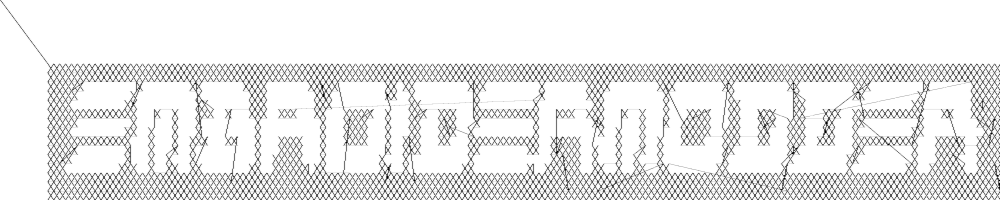
\includegraphics[width=0.5\textwidth]{images/examples/crossstitch_logo.png}

### Build

libembroidery and EmbroiderModder 2 use CMake builds
so if you are building the project to use as a library we recommend
you run:

%\lstinputlisting{examples/build_libembroidery.sh}

This builds both the static and shared versions of the library as well
as the command line program `embroider`.

\citep{packard1992pcl}
\citep{linuxcncsrc}
\citep{linuxcnc}
\citep{adobe1990postscript}
\citep{postscript1999postscript}
\citep{eduTechDST}
\citep{cups}
\citep{millOperatorsManual}
\citep{oberg1914machinery}
\citep{dxf_reference}
\citep{embroidermodder_source_code}
\citep{libembroidery_source_code}
\citep{acatina}
\citep{kde_tajima}
\citep{wotsit_archive}
\citep{wotsit_siterip}
\citep{fineemb_dst}
\citep{edutechwiki_dst}

## Graphical User Interface for PC

\label{GUI}

### Overview

*UNDER MAJOR RESTRUCTURING, PLEASE WAIT FOR VERSION 2*

Embroidermodder is a free machine embroidery application.
The newest version, Embroidermodder 2 can:

* edit and create embroidery designs
* estimate the amount of thread and machine time needed to stitch a design
* convert embroidery files to a variety of formats
* upscale or downscale designs
* run on Windows, Mac and Linux

*Embroidermodder 2* is very much a work in progress since we're doing a ground
up rewrite to an interface in C using the GUI toolkit SDL2.
The reasoning for this is detailed in the issues tab.

For a more in-depth look at what we are developing read our
website (https://www.libembroidery.org) which includes these docs as well
as the up-to date printer-friendly versions. These discuss recent changes,
plans and has user and developer guides for all the Embroidermodder projects.

To see what we're focussing on right now, see the Open Collective
News (https://opencollective.com/embroidermodder).

// fixme
This current printer-friendly version
is here (https://www.libembroidery.org/downloads/emrm.pdf).

### License

The source code is under the terms of the zlib license: see `LICENSE.md`
in the source code directory.

Permission is granted to copy, distribute and/or modify this document
under the terms of the GNU Free Documentation License, Version 1.3
or any later version published by the Free Software Foundation;
with no Invariant Sections, no Front-Cover Texts, and no Back-Cover Texts.

%A copy of the license is included in Section~\ref{GNU-free-documentation-license}.

### Build and Install

Assuming you already have the SDL2 libraries you can proceed to using the fast build, which
assumes you want to build and test locally.

The fast build should be:

```
bash build.sh
```

or, on Windows:

```
.\build.bat
```

Then run using the `run.bat` or `run.sh` scripts in the build/ directory.

Otherwise, follow the instructions below.

If you plan to install the dev version to your system (we recommend you wait
for the official installers and beta release first) then use the CMake build
instead.

### Install on Desktop

We recommend that if you want to install the development version you use the CMake build. Like
this:

```
git submodule --init --update

mkdir build
cd build
cmake ..
cmake --build .
sudo cmake --install .
```

These lines are written into the file:

```
./build_install.sh
```

On Windows use the next section.

## History

Embroidermodder 1 was started by Mark Pontius in 2004 while staying up all night
with his son in his first couple months. When Mark returned to his day job, he
lacked the time to continue the project. Mark made the decision to focus on his
family and work, and in 2005, Mark gave full control of the project to Josh
Varga so that Embroidermodder could continue its growth.

Embroidermodder 2 was conceived in mid 2011 when Jonathan Greig and Josh Varga
discussed the possibility of making a cross-platform version. It is currently in
active development and will run on GNU/Linux, Mac OS X, Microsoft Windows and
Raspberry Pi.

All Embroidermodder downloads (downloads.html) are hosted on SourceForge.

The source code for Embroidermodder 1
(\url{http://sourceforge.net/p/embroidermodder/code/HEAD/tree/embroidermodder1})
has always been hosted on Sourceforge.

The source code for Embroidermodder 2
(\url{https://github.com/Embroidermodder/Embroidermodder}) was moved to GitHub
on July 18, 2013.

The website for Embroidermodder (`embroidermodder2/docs` folder of
https://github.com/Embroidermodder/Embroidermodder) was moved to
GitHub on September 9, 2013.

## Contact us

For general questions email: \url{mailto:embroidermodder@gmail.com}.

To request a new feature  open an issue on the main Embroidermodder GitHub
repository (\url{https://github.com/Embroidermodder/Embroidermodder/issues}).
We'll move it to the correct repository.

## Downloads

### Alpha Build

This is a highly experimental build: we recommend users wait for the beta
release when the basic features are functional.

Visit our  GitHub Releases page
(\url{https://github.com/Embroidermodder/Embroidermodder/releases})
for the current build. Unfortunately, earlier builds went down with the
Sourceforge page we hosted them on.

# GUI

Embroidermodder 2 is very much a work in progress since we're doing a ground
up rewrite to an interface in Python using the GUI toolkit Tk. The reasoning for
this is detailed in the issues tab.

For a more in-depth look at what we are developing read the developer notes (link to dev notes
section). This discusses recent changes in a less formal way than a changelog (since this
software is in development) and covers what we are about to try.

## Documentation

The documentation is in the form of the website
(included in the `docs/` directory) and the printed docs in this file.

### Development

If you wish to develop with us you can chat via the contact email on the
website (\url{https://www.libembroidery.org}) or in the issues tab on the
github page (\url{https://github.com/Embroidermodder/Embroidermodder/issues}).
People have been polite and friendly in these conversations and I (Robin) have
really enjoyed them. If we do have any arguments please note we have a Code of
Conduct (\texttt{CODE\_OF\_CONDUCT.md}) so there is a consistent policy to enforce when
dealing with these arguments.

The first thing you should try is building from source using the build advice(link to build)
above. Then read some of the development notes (link to dev notes.md) to get the general
layout of the source code and what we are currently planning.

### Testing

To find unfixed errors run the tests by launching from the command line with:

```
$ embroidermodder --test
```

then dig through the output. It's currently not worth reporting the errors, since
there are so many but if you can fix anything reported here you can submit a PR.

## Code Optimisations and Simplifications

### Geometry

The geometry is stored, processed and altered via libembroidery. See the Python specific part
of the documentation for libembroidery for this. What the code in Embroidermodder does is make
the GUI widgets to change and view this information graphically.

For example if we create a circle with radius 10mm and center at `(20mm, 30mm)` then fill it
with stitches the commands would be

\lstinputlisting{examples/geometry.py}

but the user would do this through a series of GUI actions:

* Create new file
* Click add circle
* Use the Settings dialog to alter the radius and center
* Use the fill tool on circle
* Select satin from the drop down menu

So EM2 does the job of bridging that gap.

### Postscript Support

In order to safely support user contributed/shared data that can define, for
example, double to double functions we need a consistent processor for these
descriptions.

Embroidermodder backends to the postscript interpreter included in libembroidery
to accomplish this.

For example the string: `5 2 t mul add` is equivalent to
the expression $2*t + 5$.

The benefit of not allowing this to simply be a Python expression is that it is safe against
malicious use, or accidental misuse. The program can identify whether the output is of the
appropriate form and give finitely many calculations before declaring the function to have run
too long (stopping equations that hang).

To see examples of this see the \texttt{assets/shapes/*.ps} files.

### SVG Icons

To make the images easier to alter and restyle we could switch to svg icons.
There's some code in the git history to help with this.

### The Actions System

In order to simplify the development of a GUI that is flexible and easy to
understand to new developers we have a custom action system that all user
actions will go via an `actuator` that takes a string argument. By using a
string argument the undo history is just an array of strings.

The C `action\_hash\_data` struct will contain: the icon used, the
labels for the menus and tooltips and the function pointer for that action.
There will be an accompanying argument for this function call, currently being
drafted as `action\_call`. So when the user makes a function call it should
contain information like the mouse position, whether special key is pressed etc.

### Accessibility

Software can be more or less friendly to people with dyslexia, partial
sightedness, reduced mobility and those who don't speak English. Embroidermodder
2 has, in its design, the following features to help:

* icons for everything to reduce the amount of reading required
* the system font is configurable: if you have a dyslexia-friendly font you can load it
* the interface rescales to help with partial-sightedness
* the system language is configurable, unfortunately the docs will only be in English but we can try to supply lots of images of the interface to make it easier to understand as a second language
* buttons are remappable: XBox controllers are known for being good for people with reduced mobility so remapping the buttons to whatever setup you have should help

Note that most of these features will be released with version 2.1, which is planned for around
early 2023.

### Sample Files

Various sample embroidery design files can be found in the
`embroidermodder2/samples` folder.

### Shortcuts

A shortcut can be made up of zero or more modifier keys and at least one non-modifier key
pressed at once.

To make this list quickly assessable, we can produce a list of hashes which are simply the
flags ORed together.

The shortcuts are stored in the csv file `shortcuts.csv` as a 5-column table
with the first 4 columns describing the key combination. This is loaded into
the shortcuts `TABLE`. Each tick the program checks the input state for this
combination by first translating the key names into indices for the key state,
then checking for whether all of them are set to true.

### Removed Elements

So I've had a few pieces of web infrastructure fail me recently and I think
it's worth noting. An issue that affects us is an issue that can effect people
who use our software.

### Qt and dependencies

Downloading and installing Qt has been a pain for some users (46Gb on possibly
slow connections).

I'm switching to FreeGLUT 3 (which is a whole other conversation) which means
we can ship it with the source code package meaning only a basic build
environment is necessary to build it.

### Social Platform

Github is giving me a server offline (500) error and is still giving a bad ping.

So... all the issues and project boards etc. being on Github is all well and
good assuming that we have our own copies. But we don't if Github goes down or
some other major player takes over the space and we have to move (again, since
this started on SourceForge).

This file is a backup for that which is why I'm repeating myself between them.

### OpenGL

OpenGL rendering within the application. This will allow for Realistic Visualization - Bump
Mapping/OpenGL/Gradients?

This should backend to a C renderer or something.

### Configuration Data Ideas

Embroidermodder should boot from the command line regardless of whether it is or is not
installed (this helps with testing and running on machines without root). Therefore, it can
create an initiation file but it won't rely on its existence to boot:
\texttt{~/.embroidermodder/config.json}.

* Switch colors to be stored as 6 digit hexcodes with a `\#`.
* We've got close to a hand implemented ini read/write setup in `settings.py`.

### Distribution

\index{distribution}

When we release the new pip wheel we should also package:

* \texttt{.tar.gz} and \texttt{.zip} source archive.
* Debian package
* RPM package

Only do this once per minor version number.

.. todo::
   Screenshot a working draft to demonstrate.

### Perennial Jobs

* Check for memory leaks
* Clear compiler warnings on `-Wall -ansi -pedantic` for C.
* Write new tests for new code.
* Get Embroidermodder onto the current version of libembroidery.
* PEP7 compliance.
* Better documentation with more photos/screencaps.

### Full Test Suite

\index{testing}

(This needs a hook from Embroidermodder to embroider's full test suite.)

The flag `--full-test-suite` runs all the tests that have been written.
Since this results in a lot of output the details are both to stdout
and to a text file called `test\_matrix.txt`.

Patches that strictly improve the results in the `test\_matrix.txt` over
the current version will likely be accepted and it'll be a good place
to go digging for contributions. (Note: strictly improve means that
the testing result for each test is as good a result, if not better.
Sacrificing one critera for another would require some design work
before we would consider it.)

\subsection{Symbols}

\index{symbols}

Symbols use the SVG path syntax.

In theory, we could combine the icons and symbols systems, since they could be
rendered once and stored as icons in Qt. (Or as textures in FreeGLUT.)

Also we want to render the patterns themselves using SVG syntax, so it would
save on repeated work overall.

\section{Features}

\subsection{Bindings}

\index{bindings}

Bindings for libembroidery are maintained for the languages we use internally
in the project, for other languages we consider that the responsibility of
other teams using the library.

So libembroidery is going to be supported on:

\begin{itemize}
\item `C` (by default)
\item `C++` (also by default)
\item `Java` (for the Android\index{Android} application MobileViewer)
\item `Swift` (for the iOS\index{iOS} application iMobileViewer)
\end{itemize}

For `C\#` \index{C\#}\index{C-sharp} we recommend directly calling the function directly
using the DllImport feature:

```
/* Calling readCsv() via C# as a native function. */
[DllImport("libembroidery.so", EntryPoint="readCsv")]
```

see this StackOverflow discussion for help:
\hyperref{https://stackoverflow.com/questions/11425202/is-it-possible-to-call-a-c-function-from-c-net}

For Python you can do the same using ctypes:
\hyperref{https://www.geeksforgeeks.org/how-to-call-a-c-function-in-python/}

\subsection{Other Supported Thread Brands}
\index{supported threads}

The thread lists that aren't preprogrammed into formats but are indexed in
the data file for the purpose of conversion or fitting to images/graphics.

* Arc Polyester
* Arc Rayon
* Coats and Clark Rayon
* Exquisite Polyester
* Fufu Polyester
* Fufu Rayon
* Hemingworth Polyester
* Isacord Polyester
* Isafil Rayon
* Marathon Polyester
* Marathon Rayon
* Madeira Polyester
* Madeira Rayon
* Metro Polyester
* Pantone
* Robison Anton Polyester
* Robison Anton Rayon
* Sigma Polyester
* Sulky Rayon
* ThreadArt Rayon
* ThreadArt Polyester
* ThreaDelight Polyester
* Z102 Isacord Polyester

## House Style

A basic set of guidelines to use when submitting code.

### Naming Conventions

Name variables and functions intelligently to minimize the need for comments.
It should be immediately obvious what information it represents.
Short names such as x and y are fine when referring to coordinates.
Short names such as i and j are fine when doing loops.

Variable names should be \texttt{camelCase}, starting with a lowercase word followed by uppercase word(s).
C++ Class Names should be \texttt{CamelCase}, using all uppercase word(s).
C Functions that attempt to simulate namespacing, should be \texttt{"nameSpace\_camelCase"}.

All files and directories shall be lowercase and contain no spaces.

### Code Style

Tabs should not be used when indenting. Setup your IDE or text editor to use 4 spaces.

If you use KATE (KDE Advanced Text Editor), modelines are included in our code to enforce 
some of our coding standards. When creating new C/C++ files, please add
the modeline to the bottom of the file followed by a blank line. Always make sure there
is an extra blank line at the end of a file.

When using braces, please put the brace on a new line, unless the code is specially formatted
for easier reading such as a block of one liner if/else statements.

Use exceptions sparingly.

if/else is preferred over switch/case.

Do not use ternary operator (?:) in place of if/else.

Do not repeat a variable name that already occurs in an outer scope.

### Version Control

Being an open source project, developers can grab the latest code at any time
and attempt to build it themselves. We try our best to ensure that it will build smoothly
at any time, although occasionally we do break the build. In these instances,
please provide a patch, pull request which fixes the issue or open an issue and
notify us of the problem, as we may not be aware of it and we can build fine.

Try to group commits based on what they are related to: features/bugs/comments/graphics/commands/etc...

### Comments

When writing code, sometimes there are items that we know can be improved,
incomplete or need special clarification. In these cases, use the types of
comments shown below. They are pretty standard and are highlighted by many editors to
make reviewing code easier. We also use shell scripts to parse the code to find
all of these occurances so someone wanting to go on a bug hunt will be able to
easily see which areas of the code need more love.

libembroidery is written in C and adheres to C89 standards. This means
that any C99 or C++ comments will show up as errors when compiling with
gcc. In any C code, you must use:

```
/* C Style Comments */
/* TODO: This code clearly needs more work or further review. */
/* BUG: This code is definitely wrong. It needs fixed. */
/* HACK: This code shouldn't be written this way or I don't feel right about it. There may a better solution */
/* WARNING: Think twice (or more times) before changing this code. I put this here for a good reason. */
/* NOTE: This comment is much more important than lesser comments. */
```

These are rules for the general intended style of Embroidermodder's GUI source
code. Not included are anything that a compiler will warn you about: fixing
compiler warnings is more important than fixing style.

Most of this section is rationale, so skip to the end for the summary.

NEW DEVELOPERS: if your patch to Embroidermodder doesn't follow these rules,
don't worry about it. We only ask that your source code follow the basic rules
in the developer training section. These rules are for sculpting Embroidermodder
into a body of code that is resiliant to future bugs and reliable for users.

### Brevity

Readable source code is short. Developers have finite time and becoming
acquainted with more than 1000 lines of dense C code is often too high a bar
for a new developer to a project. However, this leads to a bunch of tradeoffs
that have caused issues, so instead we consider the ``minimal library``
rather than ``minimal code`` approach. Not everyone will have used the more
abstract, syntactic features of C++ like templates and operator overloading.
Even if they are capable developers with these features it makes debugging far
harder since the choice of called function is interpreted by the compiler and compiler
errors are hundred line monsters per infraction of ``these are all of the possible
variations of this function that don't match``.

Using C++'s \texttt{unordered\_map} can simplify source code in that anything can
map to anything. However, it also means we don't have to associate related structures.
For example the \texttt{action\_table} came together replacing a collection of unordered maps
with one, then replaced the mapping with labelled indices. Since the ``actuator\_core``
is a giant switch/case statement this cuts the step of identifying the action by its
label `std::string`.
The structure given by this table allowed the code to be much
easier to interpret. So for this reason we don't recommend the use unordered maps or hashes any more.

### Rigidity Vs. Ease of Modification

Difficult to restructure code is good if the structure that's there is good.
It guides new developers into safe practices without having to explain them.
Therefore we want ease of modification that comes from well chosen `structs`
and a carefully curated global header of .

### Developer Prose

### Macro Policy

Macros are great, you can do all sorts with them. But it's easy to make readable
short code that is really difficult to safely modify.

### Function Style

1. Don't write a new convenience function unless there are two existing applications of it in the source code.
2. .

### Summary

* .

## GUI Design

\index{GUI}

Embroidermodder 2 was written in C++/Qt5 and it was far too complex. We had
issues with people not able to build from source because the Qt5 libraries were
so ungainly. So I decided to do a rewrite in C/SDL2 (originally FreeGLUT, but
that was a mistake) with data stored as YAML. This means linking 4-7 libraries
depending on your system which are all well supported and widely available.

This is going well, although it's slow progress as I'm trying to keep track of
the design while also doing a ground up rewrite. I don't want to throw away good
ideas. Since I also write code for libembroidery my time is divided.

Overview of the UI rewrite

(Problems to be solved in brackets.)

It's not much to look at because I'm trying to avoid using an external
widgets system, which in turn means writing things like toolbars and menubars
over. If you want to get the design the actuator is the heart of it.

Without Qt5 we need a way of assigning signals with actions, so this is what
I've got: the user interacts with a UI element, this sends an integer to the
actuator that does the thing using the current state of the mainwindow struct
of which we expect there to be exactly one instance. The action is taken out
by a jump table that calls the right function (most of which are missing in
action and not connected up properly). It also logs the number, along with
key parts of the main struct in the undo history (an unsolved problem because
we need to decide how much data to copy over per action). This means undo,
redo and repeat actions can refer to this data.


# Introduction

The *Embroidermodder 2* project is a collection of small software utilities for
manipulating, converting and creating embroidery files in all major embroidery
machine formats. The program \textit{Embroidermodder 2} itself is a larger graphical
user interface (GUI) which is at the heart of the project.

This manual, the website (`embroidermodder.org`), mobile embroidery format viewers
and tools (`iMobileViewer`, `MobileViewer`), the core library of functions
(`libembroidery`) and CLI (`embroider`) are all tools to make the standard
user experience of working with an embroidery machine better without expensive
software which is locked to specific manufacturers and formats. But ultimately
we hope that the core \textit{Embroidermodder 2} is a practical, ever-present tool in
larger workshops, small cottage industry workshops and personal hobbyist's
bedrooms.

Embroidermodder 2 is licensed under the zlib license and we aim to keep all of
our tools open source and free of charge. If you would like to support the
project check out our Open Collective group. If you would like to help, please
join us on GitHub. This document is written as developer training as well
helping new users (see the last sections) so this is the place to learn how
to start changing the code.

# The Graphical User Interface: Embroidermodder 2.0.0-alpha

## Overview

## Features

Embroidermodder 2 has many advanced features that enable you to create awesome designs quicker, tweak existing designs to perfection, and can be fully customized to fit your workflow.

A summary of these features:

* Cross Platform
* Realistic rendering
* Various grid types and auto-adjusting rulers
* Many measurement tools
* Add text to any design
* Supports many formats
* Batch Conversion
* Scripting API

### Cross Platform

If you use multiple operating systems, it's important to choose software that works on all of them.

Embroidermodder 2 runs on Windows, Linux and Mac OS X. Let's not forget the Raspberry Pi (http://www.raspberrypi.org).

![Features: platforms](images/features-platforms-1.png)

### Realistic Rendering

It is important to be able to visualize what a design will look like when stitched and our pseudo ``3D`` realistic rendering helps achieve this.

Realistic rendering sample #1:

![Features: Real render](images/features-realrender-1.png)

Realistic rendering sample #2:

![Features: Real render](images/features-realrender-2.png)

Realistic rendering sample #3:

![Features: Real render](images/features-realrender-3.png)

### Various grid types and auto-adjusting rulers

Making use of the automatically adjusting ruler in conjunction with the grid will ensure your design is properly sized and fits within your embroidery hoop area.

Use rectangular, circular or isometric grids to construct your masterpiece!

Multiple grids and rulers in action:

![Features: Real render](images/features-grid-ruler-1.png)

### Many measurement tools

Taking measurements is a critical part of creating great designs. Whether you are designing mission critical embroidered space suits for NASA or some other far out design for your next meet-up, you will have precise measurement tools at your command to make it happen. You can locate individual points or find distances between any 2 points anywhere in the design!

Take quick and accurate measurements:

![Features: measurement](images/features-measure-1.png)

### Add text to any design

Need to make company apparel for all of your employees with individual names on them? No sweat. Just simply add text to your existing design or create one from scratch, quickly and easily.
Didn't get it the right size or made a typo? No problem. Just select the text and update it with the property editor.

Add text and adjust its properties quickly:

![Features: text](images/features-text-1.png)

### Supports many formats

Embroidery machines all accept different formats. There are so many formats available that it can sometimes be confusing whether a design will work with your machine.

Embroidermodder 2 supports a wide variety of embroidery formats as well as several vector formats, such as SVG and DXF. This allows you to worry less about which designs you can use.

### Batch Conversion

Need to send a client several different formats? Just use libembroidery-convert, our command line utility which supports batch file conversion.

There are a multitude of formats to choose from:

![Features: batch conversion](images/features-formats-1.png)

### Scripting API

If you've got programming skills and there is a feature that isn't currently available that you absolutely cannot live without, you have the capability to create your own custom commands for Embroidermodder 2. We provide an QtScript API which exposes various application functionality so that it is possible to extend the application without requiring a new release. If you have created a command that you think is worth including in the next release, just <a href=``contact.html``>contact us</a> and we will review it for functionality, bugs, and finally inclusion.

An Embroidermodder 2 command excerpt:

![Features: scripting](images/features-scripting-1.png)

## Contributing

### Version Control

Being an open source project, developers can grab the latest code at any time
and attempt to build it themselves. We try our best to ensure that it will build smoothly
at any time, although occasionally we do break the build. In these instances,
please provide a patch, pull request which fixes the issue or open an issue and
notify us of the problem, as we may not be aware of it and we can build fine.

Try to group commits based on what they are related to: features/bugs/comments/graphics/commands/etc...

See the coding style ref (coding-style)

## Introduction

### Basic Features

### Move a single stitch in an existing pattern

1. In the `File' menu, click `Open...'. When the open dialog appears find and select your file by double clicking the name of the file. Alternatively, left click the file once then click the `Open` button.
2.
3. In the `File' menu

!!! tip
    For users who prefer

### Convert one pattern to another format

1. In the `File` menu, click `Open...`.
2. The 
3. In the dropdown menu within the save dialog select the 

## Advanced Features

## Other Projects

### Planning

To see what's planned open the [Projects](https://github.com/Embroidermodder/Embroidermodder/projects/1) tab which sorts all of the GitHub Issues into columns.

### Format Support

Support for Singer FHE, CHE (Compucon) formats?

### Embroidermodder Project Coding Standards

A basic set of guidelines to use when submitting code.

### Naming Conventions

Name variables and functions intelligently to minimize the need for comments.
It should be immediately obvious what information it represents.
Short names such as ``x`` and ``y`` are fine when referring to coordinates.
Short names such as ``i`` and ``j`` are fine when doing loops.

Variable names should be `camelCase`, starting with a lowercase word followed by uppercase word(s).
C Functions that attempt to simulate namespacing, should be `nameSpace\_camelCase`.

All files and directories shall be lowercase and contain no spaces.

### Code Style

Tabs should not be used when indenting. Setup your IDE or text editor to use 4 spaces.

### Braces

For functions: please put each brace on a new line.

```
void
function_definition(int argument)
{
    /* code block */
}
```

For control statements: please put the first brace on the same line.

```
if (condition) {
    /* code block */    
}
```

Use exceptions sparingly.

Do not use ternary operator `(?:)` in place of if/else.

Do not repeat a variable name that already occurs in an outer scope.

### Version Control

Being an open source project, developers can grab the latest code at any time
and attempt to build it themselves. We try our best to ensure that it will build smoothly
at any time, although occasionally we do break the build. In these instances,
please provide a patch, pull request which fixes the issue or open an issue and
notify us of the problem, as we may not be aware of it and we can build fine.

Try to group commits based on what they are related to: features/bugs/comments/graphics/commands/etc...

### Comments

When writing code, sometimes there are items that we know can be improved,
incomplete or need special clarification. In these cases, use the types of
comments shown below. They are pretty standard and are highlighted by many editors to
make reviewing code easier. We also use shell scripts to parse the code to find
all of these occurrences so someone wanting to go on a bug hunt will be able to
easily see which areas of the code need more love. Use the same convention
as libembroidery.

libembroidery is written in C and adheres to C89 standards. This means
that any C99 or C++ comments will show up as errors when compiling with
gcc. In any C code, you must use:

```
/* C Style Comments */
/* TODO: This code clearly needs more work or further review. */
/* BUG: This code is definitely wrong. It needs fixed. */
/* HACK: This code shouldn't be written this way or I don't feel
 * right about it. There may a better solution */
/* WARNING: Think twice (or more times) before changing this code.
 * I put this here for a good reason. */
/* NOTE: This comment is much more important than lesser comments. */
```

### Donations

Creating software that interfaces with hardware is costly. A summary
of some of the costs involved:

* Developer time for 2 core developers
* Computer equipment and parts
* Embroidery machinery
* Various electronics for kitbashing Embroiderbot
* Consumable materials (thread, fabric, stabilizer, etc...)

If you have found our software useful, please consider funding further
development by donating to the project on Open Collective
(https://opencollective.com/embroidermodder).

## Introduction

!!! warning
    (UNDER MAJOR RESTRUCTURING, PLEASE WAIT FOR VERSION 2.)

Embroidermodder is a free machine embroidery application.
The newest version, Embroidermodder 2 can:

* edit and create embroidery designs
* estimate the amount of thread and machine time needed to stitch a design
* convert embroidery files to a variety of formats
* upscale or downscale designs
* run on Windows, Mac and Linux

For more information, see our website (\url{https://www.libembroidery.org})).

Embroidermodder 2 is very much a work in progress since we're doing a ground up
rewrite to an interface in Python using the GUI toolkit Tk. The reasoning for
this is detailed in the issues tab.

For a more in-depth look at what we are developing read the developer notes
\footnote{link to dev notes section}. This discusses recent changes in a less
formal way than a changelog (since this software is in development) and covers
what we are about to try.

To see what we're focussing on at the moment check this table.

|           *Date* |                                    *Event* |
|------------------|--------------------------------------------|
| April-June 2022  | Finish the conversion to C/SDL2            |
| July-August 2022 | Finish all the targets in the Design, or   |
|                  | assign them to 2.1.                        |
| September 2022   | Bugfixing, Testing, QA. libembroidery 1.0  |
|                  | will be released, then updates will slow   |
|                  | down and the Embroidermodder 2 development |
|                  | version will be fixed to the API of this   |
|                  | version.                                   |
| October 2022     | Embroidermodder 2 is officially released.  |

## Build and Install

### Desktop

First you must install the dependencies which aren't compiled into the source:

* `git`
* `cmake`
* A C compiler (we recommend `gcc` or `clang`)

on Debian Linux/GNU use:

```
$ sudo apt install git clang build-essential libsdl2-dev \
      libsdl2-images-dev libsdl2-ttf-dev
```

If you can't find a good fit for your system (on Windows use the section below),
try compiling the included submodules with:

```
$ bash build_deps.sh
```

From here, on most sytems the command:

```
$ bash build.sh
```

will build the software. Currently this is the 2.0-alpha, which will have a build code of
some kind.

### Dependencies and Build

### Plans

### Windows Specific Advice

This is one of many possible ways to build the software on Windows,
this section is to help people who've not got a build environment to start with.

1. Download and install MSYS2 (follow their instructions): https://www.msys2.org/
2. Boot ``Mintty`` from the Start menu.
3. Use the commands:

.. literalinclude:: build\_em\_on\_windows.sh
   :language: bash
   :encoding: latin-1
   :linenos:

### Mobile

These are currently unsupported (see iMobileViewer and Mobileviewer for
iOS and Android respectively), but after the Desktop version is
released we'll work on them.

The Mobile version will share some of the UI and all of the backend,
so development of the Desktop version will help us make both.

### Documentation

The documentation is in the form of the website (included in the `docs/`
directory) and the printed docs in this file.

### Development

If you wish to develop with us you can chat via the contact email
on the website (https://www.libembroidery.org) or in the issues tab on the
github page (https://github.com/Embroidermodder/Embroidermodder/issues).
People have been polite and friendly in these conversations and I (Robin)
have really enjoyed them.
If we do have any arguments please note we have a
[Code of Conduct](CODE\_OF\_CONDUCT.md) so there is a consistent policy to
enforce when dealing with these arguments.

The first thing you should try is building from source using the [build advice](link to build)
above. Then read some of the [development notes](link to dev notes.md) to get the general
layout of the source code and what we are currently planning.

## Overall Structure

## Code Optimisations and Simplifications

### Current

What Robin is currently doing.

Getting the code to pass PyLint, that involves getting all source files
under 1000 lines, renaming all variables to be in snake case.

Changing the seperation of code between EM and libembroidery.

Translating the Qt widget framework to Tk.

### Geometry

The geometry is stored, processed and altered via libembroidery. See the Python
specific part of the documentation for libembroidery for this. What the code in
Embroidermodder does is make the GUI widgets to change and view this information
graphically.

For example if we create a circle with radius 10mm and center at (20mm, 30mm)
then fill it with stitches the commands would be

```
from libembroidery import Pattern, Circle, Vector, satin
circle = Circle(Vector(20, 30), 10)
pattern = Pattern()
pattern.add_circle(circle, fill=satin)
pattern.to_stitches()
```

but the user would do this through a series of GUI actions:

1. Create new file
2. Click add circle
3. Use the Settings dialog to alter the radius and center
4. Use the fill tool on circle
5. Select satin from the drop down menu

So EM2 does the job of bridging that gap.

## Settings Dialog

There are many codeblocks for changing out the colors in one go, for example:

```
self.mw.update_all_view_select_box_colors(    self.accept["display_selectbox_left_color"],
self.accept["display_selectbox_left_fill"],
self.accept["display_selectbox_right_color"],
self.accept["display_selectbox_right_fill"],
self.preview["display_selectbox_alpha"])
```

This could be replaced with a simpler call

```
self.mw.update_all_view_select_box_colors(
self.accept["display_selectbox_colors"],
self.preview["display_selectbox_alpha"])
```

where we require that

```
self.accept["display_selectbox_colors"] == {
    "left_color": "#color",
    "left_fill": "#color",
    "right_color": "#color",
    "right_fill": "#color"
}
```

with `\#color` being some valid hex code.

### Kivy

Once the tkinter interface is up and running we can experiment
with different frontends to improve the look of the application.
For example, the MIT licensed KIVY would allow us to replace the 
mobile development in Swift and Java with all Python development:

\url{https://kivy.org/#home}

### Data/Code Seperation

All the "data" is in code files that are within the `config/`
submodule. So this way we don't have to deal with awkward data
packaging, it's just available as a single JSON style object
called `settings` available with this import line:

```
from embroidermodder.config import settings
```

In order to pass PyLint style guides this will be split up and
formatted into Python code but no processing beyond inlining
the data into a single dict should be carried out here.

### The Settings Dictionary

No more than 4 levels of indentation

Only strings, arrays, dicts and integers so matching the JSON standard. Ideally you should be able to copy/paste the data in and out and it would parse as JSON. Currently this fails because we have multi-line strings in Python syntax and inlining.

We may be able to extend the lisp support, which would deal with this. Or we can change multiline strings out for arrays of strings.

### Lisp Expression Support

In order to safely support user contributed/shared data that can
define, for example, double to double functions we need a consistent
processor for these descriptions.

Embroidermodder uses a list processor (a subset of the language
Lisp which is short for LISt Processor) to accomplish this.

For example the string: `(+ (* t 2) 5)` is equivalent to the expression: $2*t + 5$.

The benefit of not allowing this to simply be a Python expression
is that it is safe against malicious use, or accidental misuse.
The program can identify whether the output is of the appropriate
form and give finitely many calculations before declaring the
function to have run too long (stopping equations that hang).

To see examples of this see `parser.py` and `config/design\_primatives.py`.

It's also worth noting that we don't use the simpler reverse Polish
notation (RPN) approach because:

* It's more compact to use Lisp because `a b c + +` for example needs a new `+` sign for each new term as opposed to `(+ a b c)`.
* It's easier to support expressions that are themselves function calls defined by the user (by adding support for `defun` or `lambda`.

### SVG Icons

To make the images easier to alter and restyle we could switch to svg icons. There's some code in the
git history to help with this.

### The Actions System

In order to simplify the development of a GUI that is flexible and
easy to understand to new developers we have a custom action system that all
user actions will go via an `actuator` that takes a string argument. By using a
string argument the undo history is just an array of strings.

The C \texttt{action\_hash\_data} struct will contain: the icon used, the labels for the
menus and tooltips and the function pointer for that action.
There will be an accompanying argument for this function call, currently being
drafted as \texttt{action\_call}. So when the user makes a function call it should
contain information like the mouse position, whether special key is pressed
etc.

### Accessibility

Software can be more or less friendly to people with dylexia, partial sightedness,
reduced mobility and those who don't speak English.
Embroidermodder 2 has, in its design, the following features to help:

* icons for everything to reduce the amount of reading required
* the system font is configurable: if you have a dyslexia-friendly font you can load it
* the interface rescales to help with partial-sightedness
* the system language is configurable, unfortunately the docs will only be in English but we can try to supply lots of images of the interface to make it easier to understand as a second language
* buttons are remappable: XBox controllers are known for being good for people with reduced mobility so remapping the buttons to whatever setup you have should help

Note that most of these features will be released with version 2.1, which is planned for around early 2023.

### Current Work

* Converting C++ to Python throughout.
* OpenGL Rendering
  * ``Real`` rendering to see what the embroidery looks like.
  * Icons and toolbars.
  * Menu bar
* Libembroidery interfacing:
  * Get all classes to use the proper libembroidery types within them. So `Ellipse` has `EmbEllipse` as public data within it.
* Move calculations of rotation and scaling into `EmbVector` calls.
* Get undo history widget back (BUG).
* Switch website to a CMake build.
* GUI frontend for embroider features that aren't supported by embroidermodder: flag selector from a table
* Update all formats without color to check for edr or rgb files.
* EmbroideryFLOSS - Color picker that displays catalog numbers and names
* Setting for reverse scrolling direction (for zoom, vertical pan)
* Stitching simulation
* User designed custom fill
* Keyboard zooming, panning
* Advanced printing
* Libembroidery 1.0
* Better integrated help: I don't think the help should backend to a html file somewhere on the user's system. A better system would be a custom widget within the program that's searchable.
* New embroidermodder2.ico 16x16 logo that looks good at that scale.
* saving dst, pes, jef
* Settings dialog: notify when the user is switching tabs that the setting has been changed, adding apply button is what would make sense for this to happen.
* Update language translations
* Replace KDE4 thumbnailer.
* Import raster image
* Statistics from 1.0, needs histogram.
* SNAP/ORTHO/POLAR
* Cut/copy allow post-selection
* Layout into config
* Notify user of data loss if not saving to an object format.
* Add which formats to work with to preferences.
* Cannot open file with \# in the name when opening multiple files but works with opening a single file.
* Closing settings dialog with the X in the window saves settings rather than discarding them.
* Otto theme icons: units, render, selectors, what's this icon doesn't scale
* Layer manager and Layer switcher dock widget
* test that all formats read data in correct scale (format details should match other programs).
* Custom filter bug -- doesn't save changes in some cases.
* Get flake8, pylint and tests to pass.
* Sphinx documentation from docstrings or similar.

For more details read on into the Design section.

### Sample Files

Various sample embroidery design files can be found in the embroidermodder2/samples folder.

### Design

These are key bits of reasoning behind why the software is built the way it is.

### CAD command review

%cad_desc.csv


### Removed Elements

So I've had a few pieces of web infrastructure fail me recently and
I think it's worth noting. An issue that affects us is an issue that
can effect people who use our software.

### Qt and dependencies

Downloading and installing Qt has been a pain for some users
(46Gb on possibly slow connections).

I'm switching to FreeGLUT 3 (which is a whole other conversation) which means we
can ship it with the source code package meaning only a basic build
environment is necessary to build it.

### Social Platform

Github is giving me a server offline (500) error and is still giving a bad ping.

So... all the issues and project boards etc. being on Github is all well and good assuming that we have our own copies. But we don't if Github goes down or some other major player takes over the space and we have to move (again, since this started on SourceForge).

This file is a backup for that which is why I'm repeating myself between them.

### Pandoc Documentation

The documentation is, well better in that it's housed in the main repository,
but I'm not a fan of the ``write once build many`` approach as it means
trying to weigh up how 3 versions are going to render.

Can we treat the website being a duplicate of the docs a non-starter?
I'd be happier with tex/pdf only and (I know this is counter-intuitive) one
per project.

### OpenGL

OpenGL rendering within the application. This will allow for
Realistic Visualization - Bump Mapping/OpenGL/Gradients?

This should backend to a C renderer or something.

### Configuration Data Ideas

embroidermodder should boot from the command line
regardless of whether it is or is not installed (this helps with testing and
running on machines without root). Therefore, it can create an initiation file
but it won't rely on its existence to boot: `~/.embroidermodder/config.json`.

* Switch colors to be stored as 6 digit hexcodes with a \texttt{\#}.
* We've got close to a hand implemented ini read/write setup in `settings.py`.

### Distribution

When we release the new pip wheel we should also package:

* `.tar.gz` and `.zip` source archive.
* Debian package
* RPM package

Only do this once per minor version number.

### Scripting Overhaul

Originally Embroidermodder had a terminal widget, this is why we removed it.

```
> ROBIN: I think supporting scripting within Embroidermodder doesn't make sense.
> 
> All features that use scripting can be part of libembroidery instead.
> Users who are capable of using scripting won't need it, they can alter their embroidery files in CSV format, or import pyembroidery to get access.
> It makes maintaining the code a lot more complicated, especially if we move away from Qt.
> Users who don't want the scripting feature will likely be confused by it, since we say that's what libembroidery, embroider and pyembroidery are for.
> 
> How about a simpler ``call user shell`` feature? Similar to texmaker we just call system on a batch or shell script supplied by the user and it processes the file directly then the software reloads the file. Then we aren't parsing it directly.
> 
> I don't want to change this without Josh's support because it's a fairly major change.
>
> JOSH: I totally agree.
> 
> I like the idea of scripting just so people that know how to code could write their own designs without needing to fully build the app. Scripting would be a very advanced feature that most users would be confused by. Libembroidery would be a good fit for advanced features.
> 
> Now we are using Python (again, sort of) this would be a lot more natural,
> perhaps we could boot the software without blocking the shell so they can
> interact? TODO: Screenshot a working draft to demonstrate.
```

### Perennial Jobs

* Check for memory leaks
* Write new tests for new code.
* Get Embroidermodder onto the current version of libembroidery.
* PEP7 compliance.
* Better documentation with more photos/screencaps.

### Developing for Android

\url{https://developer.android.com/studio/projects/add-native-code}

```
$ apt install google-android-ndk-installer cmake lldb gradle
```

### The Command Line Interface: `embroider`

### Usage

For basic use, we recommend you build as above, then run without arguments:

```
$ embroider
```

which will print out this advice on how to use these tools without digging straight into the rest of this manual.

%.. literalinclude:: help_msg.txt

For each of the flags described here we will go into greater detail in this manual.

### To Flag

### Circle Flag

### Ellipse Flag

### Line Flag

### Polyline Flag

### Polygon Flag

### Satin Flag

### Stitch Flag

### Basic Test Suite

The flag `--test` runs the tests that take the least time and have the most utility. If you're submitting a patch for review, please run:

```
$ embroider --test | tail -n 1
```

You'll be presented with an overall PASS or FAIL for your build,
if your build fails you can try and trace the error with:

```
$ valgrind embroider --verbose --test
```

or

```
$ gdb --args embroider --verbose --test
```

depending on your preferred debugging approach. Passing this test
will be required for us to accept your patch.

### Full Test Suite

The flag `--full-test-suite` runs all the tests that have been written.
Since this results in a lot of output the details are both to stdout
and to a text file called `test\_matrix.txt`.

Patches that strictly improve the results in the `test\_matrix.txt` over
the current version will likely be accepted and it'll be a good place
to go digging for contributions. (Note: strictly improve means that
the testing result for each test is as good a result, if not better.
Sacrificing one critera for another would require some design work
before we would consider it.)

### Ideas

### Rendering system

There are two forms of render that will be produced.

1. A raster format as ppm so we can have a pixel for pixel output (for example extracting the embedded images in some formats).
2. The SVG format that will be fairly similar to InkStitch's format.

We have an EmbImage struct to store the raster format.

```
$ embroider test01.csv --render
```

currently creates a blank image. Previously the Hilbert curve test managed to
create a correctly rendered version.

#### Tactile art and braille support

One application I'd like to leave a reminder here for is automating embroidery
for blind and partially sighted people.

There are many limitations to making braille (cost, poor support, lack of
widespread adoption in the sighted world) and as such there is a strong DIY
culture around it.

There are blind internet users who can also run terminal applications using a
refreshable braille display, so in theory we could support an application like
this for them:

```
$ embroider --braille ``Hello, world!`` hello.dst
```

which would produce braille that would read `Hello, world!` as an embroidery design.

Another option is tactile fills that use the same fill algorithms but are
designed better to facilitate tactile art.

I think the way forward on this is to call up the RNIB business advice line and ask for assistance once we have a working model. That way they can get us in contact with experts to review how legible the output is and usable the software is for the intended audience.

This is less important than getting better machine support but given the high social impact I think it should be a priority.

### The Low Level API: Libembroidery 1.0.0-alpha

### API Reference

### `convert`


### Mobile Support: MobileViewer and iMobileViewer

### Embroidermodder 2.0.0-alpha User Manual

### Introduction

### Basic Features

### Move a single stitch in an existing pattern

1. In the `File` menu, click `Open...`. When the open dialog appears find and select your file by double clicking the name of the file. Alternatively, left click the file once then click the `Open` button.
2. 
3. In the `File` menu

TIP: For users who prefer

### Convert one pattern to another

1. In the `File` menu, click `Open...`.
2.  The
3.  In the dropdown menu within the save dialog select the

### Advanced Features

### Other Projects

### References

### Ideas

### Why this document

I've been trying to make this document indirectly through the Github
issues page and the website we're building but I think a
straightforward, plain-text file needs to be the ultimate backup for
this. Then I can have a printout while I'm working on the project.

### Issues

### Fix before Version 2

So I've had a few pieces of web infrastructure fail me recently and I
think it's worth noting. An issue that affects us is an issue that can
effect people who use our software.

1. Googletests require a web connection to update and they update on each compilation.
2. Downloading and installing Qt has been a pain for some users (46Gb on possibly slow connections). I think it was davieboy64?
3. The documentation is, well better in that it's housed in the main repository, but I'm not a fan of the ``write once build many`` approach as it means trying to weigh up how 3 versions are going to render.
4. Github is giving me a server offline (500) error and is still giving a bad ping.
5. OpenGL rendering within the application. This will allow for Realistic Visualization - Bump Mapping/OpenGL/Gradients?
6. JSON configuration (Started, see \texttt{head -n 50 src/mainwindow.cpp}.) Ok this is changing slightly. embroidermodder should boot from the command line regardless of whether it is or is not installed (this helps with testing and running on machines without root). Therefore, it can create an initiation file but it won't rely on its existence to boot: this is what we currently do with settings.ini.
7. Get undo history widget back (BUG).
8. Switch website to a CMake build.
9. Mac Bundle, .tar.gz and .zip source archive.
10. NSIS installer for Windows, Debian package, RPM package
11. GUI frontend for embroider features that aren't supported by embroidermodder: flag selector from a table
12. Update all formats without color to check for edr or rgb files.
13. EmbroideryFLOSS - Color picker that displays catalog numbers and names
14. Setting for reverse scrolling direction (for zoom, vertical pan)
15. Stitching simulation
16. User designed custom fill
17. Keyboard zooming, panning
18. Advanced printing
19. Libembroidery 1.0
20. Better integrated help: I don't think the help should backend to a html file somewhere on the user's system. A better system would be a custom widget within the program that's searchable.
21. New embroidermodder2.ico 16x16 logo that looks good at that scale.
22. saving dst, pes, jef
23. Settings dialog: notify when the user is switching tabs that the setting has been changed, adding apply button is what would make sense for this to happen.
24. Update language translations
25. Replace KDE4 thumbnailer.
26. Import raster image
27. Statistics from 1.0, needs histogram.
28. SNAP/ORTHO/POLAR
29. Cut/copy allow post-selection
30. Layout into config
31. Notify user of data loss if not saving to an object format.
32. Add which formats to work with to preferences.
33. Cannot open file with \# in the name when opening multiple files but works with opening a single file.
34. Closing settings dialog with the X in the window saves settings rather than discarding them.
35. Otto theme icons: units, render, selectors, what's this icon doesn't  scale
36. Layer manager and Layer switcher dock widget
37. Test that all formats read data in correct scale (format details should match other programs).
38. Custom filter bug -- doesn't save changes in some cases.

### Fix for Version 2.1

### Fix eventually

### googletests

gtests are non-essential, testing is for developers not users so we can
choose our own framework. I think the in-built testing for libembroidery
was good and I want to re-instate it.

### Qt and dependencies

I'm switching to SDL2 (which is a whole other conversation) which means
we can ship it with the source code package meaning only a basic build
environment is necessary to build it.

### Documentation

Can we treat the website being a duplicate of the docs a non-starter?
I'd be happier with tex/pdf only and (I know this is counter-intuitive)
one per project.

### Social Platform

So... all the issues and project boards etc. being on Github is all well and good assuming that we have our own copies. But we don't if Github goes down or some other major player takes over the space and we have to move (again, since this started on SourceForge).

This file is a backup for that which is why I'm repeating myself between them.

### JSON data Ideas

So:

1. Port `settings.ini` to `settings.json`.
2. Place `settings.json` in `\$HOME/.embroidermodder` (or equivalent, see the homedir function in \texttt{gui.c}).
3. Parse JSON using cJSON (we have the new parseJSON function).
4. Better structure for settings data so parse and load JSON is easier and
   there's less junk in global variables. A structure similar to a
5. Python dict that uses constants like the sketch below.

### Why JSON over ini?

1. We need find _a_ new system because the current system is Qt dependent anyway.
2. This way we can store more complex data structures in the same system including the layout of the widgets which may be user configured (see Blender and GIMP).
3. Also it's easier to share information formatted this way between systems because most systems us JSON or XML data: there's better support for converting complex data this way.

### Sketch of a settings system

.. literalinclude:: examples/settings\_system.c

This would all be in C, and wouldn't rely on Qt at all. We already use a
system like this in `libembroidery` so hopefully devs on both
would get the pattern.

\subsection{Design}

These are key bits of reasoning behind why the software is built the way it is.

\subsection{Scripting Overhaul}

Originally Embroidermodder had a terminal widget, this is why we removed it.

\begin{quote}
ROBIN: I think supporting scripting within Embroidermodder doesn't make
sense.

All features that use scripting can be part of libembroidery instead.
Users who are capable of using scripting won't need it, they can alter
their embroidery files in CSV format, or import pyembroidery to get
access. It makes maintaining the code a lot more complicated, especially
if we move away from Qt. Users who don't want the scripting > feature will
likely be confused by it, since we say that's what  libembroidery,
embroider and pyembroidery are for.

How about a simpler ``call user shell`` feature? Similar to texmaker we
just call system on a batch or shell script supplied by the user and it
processes the file directly then the software reloads the file. Then we
aren't parsing it directly.

I don't want to change this without Josh's support because it's a fairly
major change.

JOSH: I totally agree.

I like the idea of scripting just so people that know how to code could
write their own designs without needing to fully build the app.
Scripting would be a very advanced feature that most users would be
confused by. Libembroidery would be a good fit for advanced features.
\end{quote}

### Perennial Jobs

1. Check for memory leaks
2. Clear compiler warnings on `-Wall\ -ansi\ -pedantic` for C.

\subsection{Developing for Android}

https://developer.android.com/studio/projects/add-native-code

```
apt install google-android-ndk-installer cmake lldb gradle
```

### Bibilography

### Introduction

### Basic Features

### Move a single stitch in an existing pattern

1. In the `File` menu, click `Open...`. When the open dialog appears find and select your file by double clicking the name of the file. Alternatively, left click the file once then click the `Open` button.
2. .
3. In the `File` menu

TIP: For users who prefer

### Convert one pattern to another format

* In the `File` menu, click `Open...`.
* The
* In the dropdown menu within the save dialog select the

### Advanced Features

### Other Projects

### References

### Planning

To see what's planned open the
[Projects](https://github.com/Embroidermodder/Embroidermodder/projects/1)
tab which sorts all of the GitHub Issues into columns.

### Format Support

Support for Singer FHE, CHE (Compucon) formats?

### Embroidermodder Project Coding Standards

A basic set of guidelines to use when submitting code.

### Naming Conventions

Name variables and functions intelligently to minimize the need for
comments. It should be immediately obvious what information it
represents. Short names such as x and y are fine when referring to
coordinates. Short names such as i and j are fine when doing loops.

Variable names should be "camelCase", starting with a lowercase word
followed by uppercase word(s). C++ Class Names should be "CamelCase",
using all uppercase word(s). C Functions that attempt to simulate namespacing,
should be ``nameSpace\_camelCase``.

All files and directories shall be lowercase and contain no spaces.

### Code Style

Tabs should not be used when indenting. Setup your IDE or text editor to use 4 spaces.

### Braces

For functions: please put each brace on a new line.

```
void function\_definition(int argument)
{

}
```

For control statements: please put the first brace on the same line.

```
if (condition) {

}
```

Use exceptions sparingly.

Do not use ternary operator (?:) in place of if/else.

Do not repeat a variable name that already occurs in an outer scope.

### Version Control

Being an open source project, developers can grab the latest code at any
time and attempt to build it themselves. We try our best to ensure that
it will build smoothly at any time, although occasionally we do break
the build. In these instances, please provide a patch, pull request
which fixes the issue or open an issue and notify us of the problem, as
we may not be aware of it and we can build fine.

Try to group commits based on what they are related to:
features/bugs/comments/graphics/commands/etc...

### Comments

When writing code, sometimes there are items that we know can be
improved, incomplete or need special clarification. In these cases, use
the types of comments shown below. They are pretty standard and are
highlighted by many editors to make reviewing code easier. We also use
shell scripts to parse the code to find all of these occurrences so
someone wanting to go on a bug hunt will be able to easily see which
areas of the code need more love.

libembroidery is written in C and adheres to C89 standards. This means
that any C99 or C++ comments will show up as errors when compiling with
gcc. In any C code, you must use:

```
/* C Style Comments */
/* TODO: This code clearly needs more work or further review. */
/* BUG: This code is definitely wrong. It needs fixed. */
/* HACK: This code shouldn't be written this way or I don't feel right about it. There may a better solution */
/* WARNING: Think twice (or more times) before changing this code. I put this here for a good reason. */
/* NOTE: This comment is much more important than lesser comments. */
```

## Ideas

### Why this document

I've been trying to make this document indirectly through the Github
issues page and the website we're building but I think a
straightforward, plain-text file needs to be the ultimate backup for
this. Then I can have a printout while I'm working on the project.

### Issues

#### Fix before Version 2

So I've had a few pieces of web infrastructure fail me recently and I
think it's worth noting. An issue that affects us is an issue that can
effect people who use our software.

* Googletests require a web connection to update and they update on each compilation.
* Downloading and installing Qt has been a pain for some users (46Gb on possibly slow connections). I think it was davieboy64?
* Github is giving me a server offline (500) error and is still giving a bad ping.
* OpenGL rendering within the application. This will allow for Realistic Visualization - Bump Mapping/OpenGL/Gradients?
* JSON configuration (Started, see \texttt{head\ -n\ 50\ src/mainwindow.cpp.}) Ok this is changing slightly. embroidermodder should boot from the command line regardless of whether it is or is not installed (this helps with testing and running on machines without root). Therefore, it can create an initiation file but it won't rely on its existence to boot: this is what we currently do with settings.ini.
* Get undo history widget back (BUG).
* Switch website to a CMake build.
* Mac Bundle, .tar.gz and .zip source archive.
* NSIS installer for Windows, Debian package, RPM package
* GUI frontend for embroider features that aren't supported by  embroidermodder: flag selector from a table
* Update all formats without color to check for edr or rgb files.
* EmbroideryFLOSS - Color picker that displays catalog numbers and names
* Setting for reverse scrolling direction (for zoom, vertical pan)
* Stitching simulation
* User designed custom fill
* Keyboard zooming, panning
* Advanced printing
* Libembroidery 1.0
* Better integrated help: I don't think the help should backend to a html file somewhere on the user's system. A better system would be a custom widget within the program that's searchable.
* New embroidermodder2.ico 16x16 logo that looks good at that scale.
* saving dst, pes, jef
* Settings dialog: notify when the user is switching tabs that the setting has been changed, adding apply button is what would make sense for this to happen.
* Update language translations
* Replace KDE4 thumbnailer.
* Import raster image
* Statistics from 1.0, needs histogram.
* SNAP/ORTHO/POLAR
* Cut/copy allow post-selection
* Layout into config
* Notify user of data loss if not saving to an object format.
* Add which formats to work with to preferences.
* Cannot open file with \# in the name when opening multiple files but  works with opening a single file.
* Closing settings dialog with the X in the window saves settings rather than discarding them.
* Otto theme icons: units, render, selectors, what's this icon doesn't scale
* Layer manager and Layer switcher dock widget
*  test that all formats read data in correct scale (format details should match other programs).
* Custom filter bug -- doesn't save changes in some cases.

#### Social Platform

So... all the issues and project boards etc. being on Github is all
well and good assuming that we have our own copies. But we don't if
Github goes down or some other major player takes over the space and we
have to move (again, since this started on SourceForge).

This file is a backup for that which is why I'm repeating myself between
them.

### JSON data Ideas

So:

1. Port `settings.ini` to `settings.json`.
2. Place `settings.json` in `\$HOME/.embroidermodder` (or equivalent, see the homedir function in `gui.c`).
3. Parse JSON using cJSON (we have the new parseJSON function).
4. Better structure for settings data so parse and load JSON is easier and there's less junk in global variables. A structure similar to a Python dict that uses constants like the sketch below.

#### Why JSON over ini?

1. We need to hand-write \emph{a} system because the current system is Qt dependent anyway.
2. This way we can store more complex data structures in the same system including the layout of the widgets which may be user configured (see Blender and GIMP).
3. Also it's easier to share information formatted this way between systems because most systems us JSON or XML data: there's better support for converting complex data this way.

#### Sketch of a settings system

%.. literalinclude:: examples/settings\_system.c

This would all be in C, and wouldn't rely on Qt at all. We already use a
system like this in \texttt{libembroidery} so hopefully devs on both
would get the pattern.

### Design

These are key bits of reasoning behind why the software is built the way
it is.

## Conclusions

## Bibliography

The Embroidermodder Team \emph{Embroidermodder}
\url{http://www.libembroidery.org} (accessed 3. June. 2022)

achatina *Technical Info*
\url{http://www.achatina.de/sewing/main/TECHNICL.HTM} (accessed 28. Sep. 2021)

KDE Community
**Projects/Liberty/File Formats/Tajima Ternary - KDE Community Wiki**
\url{https://community.kde.org/Projects/Liberty/File_Formats/Tajima_Ternary}
(accessed 28. Sep. 2021)

FineEmb Studio
**FineEmb Studio \guillemotright DST**
\url{https://www.fineemb.com/blog/archives/dst-file-encoding.html}
(accessed 28. Sep. 2021)

EduTech Wiki
**Embroidery format DST - EduTech Wiki**
\url{https://edutechwiki.unige.ch/en/Embroidery_format_DST}
(accessed 28. Sep. 2021)

# Color Charts

## Built-ins

### SVG Colors

## Threads

### DXF color table

### HUS color table

### JEF color table

### PCM color table

### PEC color table

## Contributing

### Version Control

Being an open source project, developers can grab the latest code at any time
and attempt to build it themselves. We try our best to ensure that it will build smoothly
at any time, although occasionally we do break the build. In these instances,
please provide a patch, pull request which fixes the issue or open an issue and
notify us of the problem, as we may not be aware of it and we can build fine.

Try to group commits based on what they are related to: features/bugs/comments/graphics/commands/etc...

See the coding style  here (coding-style).

### Get the Development Build going

When we switch to releases we recommend using them, unless you're reporting a bug in which case you can check the development build for whether it has been patched. If this applies to you, the current development build is https://github.com/Embroidermodder/Embroidermodder/releases/tag/alpha3[here].

### To Do

* Beta
  * Libembroidery 1.0.
  * Better integrated help: I don't think the help should backend to a html file somewhere on the user's system. A better system would be a custom widget within the program that's searchable.
  * EmbroideryFLOSS - Color picker that displays catalog numbers and names.
  * Custom filter bug -- doesn't save changes in some cases.
  * Advanced printing.
  * Stitching simulation.
* 2.x/ideas
  * User designed custom fill.

These are key bits of reasoning behind why the GUI is built the way it is.

## Translation of the user interface

In a given table the left column is the default symbol and the right string is the translation.
If the translate function fails to find a translation it returns the default symbol.

So in US English it is an empty table, but in UK English
only the dialectical differences are present.

Ideally, we should support at least the 6 languages spoken at the UN. Quoting
https://www.un.org

> _There are six official languages of the UN. These are Arabic, Chinese, English, French, Russian and Spanish._

We're adding Hindi, on the grounds that it is one of the most commonly spoken languages and at
least one of the Indian languages should be present.

Written Chinese is generally supported as two different symbol sets and we follow that
convension.

English is supported as two dialects to ensure that the development team is aware of what those
differences are. The code base is written by a mixture of US and UK native English speakers
meaning that only the variable names are consistently one dialect: US English. As for
documentation: it is whatever dialect the writer prefers (but they should maintain consistency
within a text block like this one).

Finally, we have \texttt{default}, which is the dominant language
of the internals of the software. Practically, this is
just US English, but in terms of programming history this
is the \texttt{C locale}.

### Old action system notes

Action: the basic system to encode all user input.

This typedef gives structure to the data associated with each action
which, in the code, is referred to by the action id (an int from
the define table above).

### DESCRIPTION OF STRUCT CONTENTS

### label

The action label is always in US English, lowercase,
seperated with hyphens.

For example: \texttt{new-file}.

## Flags

The bit based flags all collected into a 32-bit integer.

| bit(s) | description |
|----|-----------------------|
| 0 | User (0) or system (1) permissions. |
| 1-3 | The mode of input. |
| 4-8 | The object classes that this action can be applied to. |
| 9-10 | What menu (if any) should it be present in. |
| 11-12 | What |

\caption{Flags of EM actions}

### Description

The string placed in the tooltip describing the action.

### Original Prompt System

NOTE: `main()` is run every time the command is started.
Use it to reset variables so they are ready to go.

NOTE: `click()` is run only for left clicks.
Middle clicks are used for panning.
Right clicks bring up the context menu.

NOTE: `move()` is optional. It is run only after
`enableMoveRapidFire()` is called. It
will be called every time the mouse moves until
`disableMoveRapidFire()` is called.

NOTE: `prompt()` is run when Enter is pressed.
`appendPromptHistory` is automatically called before `prompt()`
is called so calling it is only needed for erroneous input.
Any text in the command prompt is sent as an uppercase string.

# Libembroidery v1.0-alpha

(Under construction, please wait for v1.0 release.)

Libembroidery is a low-level library for reading, writing, 
and altering digital embroidery files in C. It is part of the Embroidermodder Project
for open source machine embroidery.

Libembroidery is the underlying library that is used by [Embroidermodder 2](http://embroidermodder.org)
and is developed by [The Embroidermodder Team](ref the-embroidermodder-team).
A full list of contributors to the project is maintained in
[the Embroidermodder 2 github](https://github.com/Embroidermodder/embroidermodder)
in the file `CREDITS.md`.
It handles over 45 different embroidery specific formats as well
as several non-embroidery specific vector formats.

It also includes a CLI called `embroider` that allows for better automation of
changes to embroidery files and will be more up-to date than
the Embroidermodder 2 GUI.

## Documentation

Libembroidery is documented as part of the [Embroidermodder 2.0 manual](
\url{https://www.libembroidery.org/emrm-2.0.0-alpha.pdf}).
If you need libembroidery for any non-trivial usage or want to contribute to
the library we advise you read the appropriate design sections of the manual
first. Copies of this manual will be shipped with the packaged version of
libembroidery, but to build it we use the Doxyfile in [the Embroidermodder git
repository](https://github.com/Embroidermodder/embroidermodder).

For more basic usage, `embroider` should have some in-built help starting with:

```
$ embroider --help
```

### License

Libembroidery is distributed under the permissive zlib licence, see the LICENCE file.

### Demos

We're currently trying out some fill techniques which will be demonstrated here
and in the script \texttt{qa\_test.sh}.


\includegraphics[width=0.5\textwidth]{images/logo-spirals.png}

Converts to:

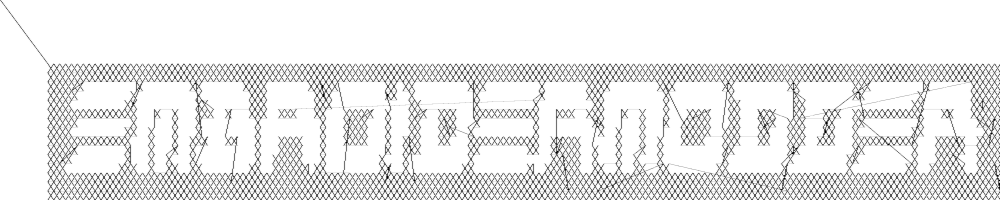
\includegraphics[width=0.5\textwidth]{images/logo_spirals_cross_stitch.png}

### Build

libembroidery and EmbroiderModder 2 use CMake builds
so if you are building the project to use as a library we recommend
you run:

.. literalinclude:: ../bin/build\_libembroidery.sh
   :language: bash
   :encoding: latin-1
   :linenos:

This builds both the static and shared versions of the library as well
as the command line program `embroider`.

### Changelog

### Ideas

Stuff that is now supposed to be generated by Doxygen:

* todo: Bibliography style to plainnat.
* todo: US letter paper version of printed docs.

# Formats

## Overview

### Read/Write Support Levels

The table of read/write format support levels uses the status levels described here:
%\if{0}

\begin{longtable}{p{4cm} p{8cm}}
\caption{Read/Write Support Levels.}
\label{tab:read-write-support} \\
\textbf{Status Label} &
\textbf{Description} \\

\texttt{rw-none} &
Either the format produces no output, reporting an error. Or it produces a
Tajima dst file as an alternative. \\

\texttt{rw-poor} &
A file somewhat similar to our examples is produced. We don't know how well
it runs on machines in practice as we don't have any user reports or personal
tests. \\

\texttt{rw-basic} &
Simple files in this format run well on machines that use this format. \\

\texttt{rw-standard} &
Files with non-standard features work on machines and we have good documentation
on the format. \\

\texttt{rw-reliable} &
All known features don't cause crashes. Almost all work as expected. \\

\texttt{rw-complete} &
All known features of the format work on machines that use this format.
Translations from and to this format preserve all features present in both.
\end{longtable}

These can be split into `r-basic w-none`, for example, if they don't match.

So all formats can, in principle, have good read and good write support, because it's defined in relation to files that we have described the formats for.

### Test Support Levels

| Status Label | Description             |
|--------------|-------------------------|
| `test-none` | No tests have been written to test the specifics of the format. |
| `test-basic` | Stitch Lists and/or colors have read/write tests. |
| `test-thorough` | All features of that format has at least one test. |
| `test-fuzz` | Can test the format for uses of features that we haven't thought of by feeding in nonsense that is designed to push possibly dangerous weaknesses to reveal themselves. |
| `test-complete` | Both thorough and fuzz testing is covered. |

So all formats can, in principle, have complete testing support, because it's
defined in relation to files that we have described the formats for.

### Documentation Support Levels

| Status Label | Description             |
|--------------|-------------------------|
| `doc-none` | We haven't researched this beyond finding example files. |
| `doc-basic` | We have a rough sketch of the size and contents of the header if there is one. We know the basic stitch encoding (if there is one), but not necessarily all stitch features. |
| `doc-standard` | We know some good sources and/or have tested all the features that appear to exist. They mostly work the way we have described. |
| `doc-good` | All features that were described somewhere have been covered here or we have thoroughly tested our ideas against other softwares and hardwares and they work as expected. |
| `doc-complete` | There is a known official description and our description covers all the same features. |

Not all formats can have complete documentation because it's based on what
information is publically available. So the total score is reported in the table
below based on what level we think is available.

### Overall Support

Since the overall support level is the combination of these
4 factors, but rather than summing up their values it's an
issue of the minimum support of the 4.

| Status Label | Description             |
|--------------|-------------------------|
| `read-only` | If write support is none and read support is not none. |
| `write-only` | If read support is none and write support is not none. |
| `unstable` | If both read and write support are not none but testing or documentation is none. |
| `basic` | If all ratings are better than none. |
| `reliable` | If all ratings are better than basic. |
| `complete` | If all ratings could not reasonably be better (for example any improvements rely on information that we may never have access to). This is the only status that can be revoked, since if the format changes or new documentation is released it is no longer complete. |
| `experimental` | For all other scenarios. |

### Table of Format Support Levels

Overview of documentation support by format.

``.. csv-table::``
``:file: format\_support.csv``

.. literalinclude:: format\_support.csv

* TODO Josh, Review this section and move any info still valid or needing work into TODO comments in the actual libembroidery code. Many items in this list are out of date and do not reflect the current status of libembroidery. When finished, delete this file.
  * Test that all formats read data in correct scale (format details should match other programs)
  * Add which formats to work with to preferences.
  * Check for memory leaks
  * Update all formats without color to check for edr or rgb files
  * Fix issues with DST (VERY important that DST work well)
* todo Support for Singer FHE, CHE (Compucon) formats?

## Geometry and Algorithms

### To Do

### Arduino

* Fix emb-outline files
* Fix thread-color files
* Logging of Last Stitch Location to External USB Storage(commonly available and easily replaced) ...wait until TRE is available to avoid rework
* inotool.org - seems like the logical solution for Nightly/CI builds
* Smoothieboard experiments

### Testing

* looping test that reads 10 times while running valgrind. See ``embPattern\_loadExternalColorFile()`` Arduino leak note for more info.

### Development

If you wish to develop with us you can chat via the contact email
on the website https://libembroidery.org or in the issues tab on the
github page https://github.com/Embroidermodder/Embroidermodder/issues.
People have been polite and friendly in these conversations and I (Robin)
have really enjoyed them.
If we do have any arguments please note we have a
Code of Conduct ``CODE\_OF\_CONDUCT.md`` so there is a consistent policy to
enforce when dealing with these arguments.

The first thing you should try is building from source using the  build advice (build)
above. Then read some of the
[manual](https://libembroidery.org/downloads/emrm.pdf) to get the general
layout of the source code and what we are currently planning.

## Contributing

### Funding

The easiest way to help is to fund development (see the Donate button above),
since we can't afford to spend a lot of time developing and only have limited
kit to test out libembroidery on.

### Programming and Engineering

Should you want to get into the code itself:

* Low level C developers are be needed for the base library \texttt{libembroidery}.
* Low level assembly programmers are needed for translating some of `libembroidery` to `EmbroiderBot`.
* Hardware Engineers to help design our own kitbashed embroidery machine `EmbroiderBot`, one of the original project aims in 2013.
* Scheme developers and C/SDL developers to help build the GUI.
* Scheme developers to help add designs for generating of custom stitch-filled emblems like the heart or dolphi. Note that this happens in Embroidermodder not libembroidery (which assumes that you already have a function available).

### Writing

We also need people familiar with the software and the general
machine embroidery ecosystem to contribute to the
documentation (https://github.com/Embroidermodder/www.libembroidery.org).

We need researchers to find references for the documentation: colour tables,
machine specifications etc. The history is murky and often very poorly maintained
so if you know anything from working in the industry that you can share: it'd be
appreciated!

## Embroidermodder Project Coding Standards

A basic set of guidelines to use when submitting code.

Code structure is mre important than style, so first we advise you read
"Design" and experimenting before getting into the specifics of code style.

### Where Code Goes

Anything that deals with the specifics of embroidery file formats, threads,
rendering to images, embroidery machinery or command line interfaces should go 
in `libembroidery` not here.

### Where Non-compiled Files Go

.. todo::
   Like most user interfaces Embroidermodder is mostly data,
   so here we will have a list describing where each CSV goes.

### Ways in which we break style on purpose

Most style guides advise you to keep functions short. We make a few pointed
exceptions to this where the overall health and functionality of the source code should benefit.

The `actuator` function will always be a mess and it should be: we're keeping
the total source lines of code down by encoding all user action into a descrete
sequence of strings that are all below \texttt{``\_STRING\_LENGTH``} in length. See
the section on the actuator (TODO) describing why any other solution we could
think  here would mean more more code without a payoff in speed of execution or
clarity.

## Version Control

Being an open source project, developers can grab the latest code at any time and attempt to build it themselves. We try our best to ensure that it will build smoothly at any time, although occasionally we do break the build. In these instances, please provide a patch, pull request which fixes the issue or open an issue and notify us of the problem, as we may not be aware of it and we can build fine.

Try to group commits based on what they are related to: features/bugs/comments/graphics/commands/etc...

## Donations

Creating software that interfaces with hardware is costly. A summary of some of the costs involved:

* Developer time for 2 core developers
* Computer equipment and parts
* Embroidery machinery
* Various electronics for kitbashing Embroiderbot
* Consumable materials (thread, fabric, stabilizer, etc...)

If you have found our software useful, please consider funding further development by donating to the project on Open Collective
(\url{https://opencollective.com/embroidermodder}).

## Embroidermodder Project Coding Standards

Rather than maintain our own standard for style, please defer to
the Python's PEP 7 %\citep{pep7}
for C style and emulating that in C++.

A basic set of guidelines to use when submitting code. Defer to the PEP7 standard with the following additions:

* All files and directories shall be lowercase and contain no spaces.
* Structs and class names should use `LeadingCapitals`.
* Enums and constants should be `BLOCK\_CAPITALS`.
* Class members and functions without a parent class should be `snake\_case`. With the exception of when one of the words is a ``class`` name from libembroidery in which case it has the middle capitals like this: `embArray\_add`.
* Don't use exceptions.
* Don't use ternary operator (?:) in place of if/else.
* Don't repeat a variable name that already occurs in an outer scope.

## Version Control

Being an open source project, developers can grab the latest code at any
time and attempt to build it themselves. We try our best to ensure that
it will build smoothly at any time, although occasionally we do break
the build. In these instances, please provide a patch, pull request
which fixes the issue or open an issue and notify us of the problem, as
we may not be aware of it and we can build fine.

Try to group commits based on what they are related to:
features/bugs/comments/graphics/commands/etc...

### Comments

When writing code, sometimes there are items that we know can be
improved, incomplete or need special clarification. In these cases, use
the types of comments shown below. They are pretty standard and are
highlighted by many editors to make reviewing code easier. We also use
shell scripts to parse the code to find all of these occurrences so
someone wanting to go on a bug hunt will be able to easily see which
areas of the code need more love.

libembroidery and Embroidermodder are written in C and adheres to C89 standards. This means
that any C99 or C++ comments will show up as errors when compiling with
gcc. In any C code, you must use:

.. literalinclude:: examples/comment.c

### Ideas

## Why this document

I've been trying to make this document indirectly through the Github
issues page and the website we're building but I think a
straightforward, plain-text file needs to be the ultimate backup for
this. Then I can have a printout while I'm working on the project.

### Qt and dependencies

I'm switching to SDL2 (which is a whole other conversation) which means
we can ship it with the source code package meaning only a basic build
environment is necessary to build it.

### Documentation

Can we treat the website being a duplicate of the docs a non-starter?
I'd be happier with tex/pdf only and (I know this is counter-intuitive)
one per project.

### Social Platform

So... all the issues and project boards etc. being on Github is all
well and good assuming that we have our own copies. But we don't if
Github goes down or some other major player takes over the space and we
have to move (again, since this started on SourceForge).

This file is a backup for that which is why I'm repeating myself between
them.

### Identify the meaning of these TODO items

.. todo::
   Saving CSV/SVG (rt) + CSV read/write UNKNOWN interpreted as COLOR bug `\#179`

.. todo::
   Lego Mindstorms NXT/EV3 ports and/or commands

### Progress Chart

The chart of successful from-to conversions (previously a separate issue)
is something that should appear in the README.

### Standard

The criteria for a good Pull Request from an outside developer has these properties, from most to least important:

* No regressions on testing.
* Add a feature, bug fix or documentation that is already agreed on through GitHub issues or some other way with a core developer.
* No GUI specific code should be in libembroidery, that's for Embroidermodder.
* Pedantic/ansi C unless there's a good reason to use another language.
* Meet the style above (i.e.  PEP 7, Code Lay-out \footnote{\url{https://peps.python.org/pep-0007/#code-lay-out}}. We'll just fix the style if the code's good and it's not a lot of work.
* \texttt{embroider} should be in POSIX style as a command line program.
* No dependancies that aren't ``standard``, i.e. use only the C Standard Library.

## Image Fitting

A currently unsolved problem in development that warrants further research is
the scenario where a user wants to feed embroider an image that can then be .

### To Place

A *right-handed coordinate system* \index{right-handed coordinate system}
is one where up is positive and right is
positive. Left-handed is up is positive, left is positive. Screens often use
down is positive, right is positive, including the OpenGL standard so when
switching between graphics formats and stitch formats we need to use a vertical
flip (`embPattern\_flip`).

`0x20` is the space symbol, so when padding either 0 or space is preferred and
in the case of space use the literal ' '.

### To Do

We currently need help with:

* Thorough descriptions of each embroidery format.
* Finding resources for each of the branded thread libraries (along with a full citation for documentation).
* Finding resources for each geometric algorithm used (along with a full citation for documentation).
* Completing the full `--full-test-suite` with no segfaults and at least a clear error message (for example ``not implemented yet``).
* Identifying ``best guesses`` for filling in missing information when going from, say ``.csv`` to a late ``.pes`` version. What should the default be when the data doesn't clarify?
* Improving the written documentation.
* Funding, see the Sponsor button above. We can treat this as ``work`` and put far more hours in with broad support in small donations from people who want specific features.

Beyond this the development targets are categories sorted into:

* Basic Features
* Code quality and user friendliness
* embroider CLI
* Documentation
* GUI
* electronics development

### Basic features

* Incorporate `\#if 0` ed parts of `libembroidery.c`.
* Interpret how to write formats that have a read mode from the source code and vice versa.
* Document the specifics of the file formats here for embroidery machine specific formats. Find websites and other sources that break down the binary formats we currently don't understand.
* Find more and better documentation of the structure of the headers for the formats we do understand.

### Code quality and user friendliness

* Document all structs, macros and functions (will contribute directly on the web version).
* Incorporate experimental code, improve support for language bindings.
* Make stitch x, y into an EmbVector.

### Documentation

Run `sloccount` on `extern/` and `.` (and ) so we know the
current scale of the project, aim to get this number low. Report the total as
part of the documentation.

Try to get as much of the source code that we maintain into C as possible so
new developers don't need to learn multiple languages to have an effect. This
bars the embedded parts of the code.

### GUI

* Make EmbroideryMobile (Android) also backend to `libembroidery` with a Java wrapper.
* Make EmbroideryMobile (iOS) also backend to `libembroidery` with a Swift wrapper.
* Share some of the MobileViewer and iMobileViewer layout with the main EM2. Perhaps combine those 3 into the Embroidermodder repository so there are 4 repositories total.
* Convert layout data to JSON format and use cJSON for parsing.

## Development

### Contributing

If you're interested in getting involved, here's some guidance
for new developers. Currently The Embroidermodder Team is all
hobbyists with an interest in making embroidery machines more
open and user friendly. If you'd like to support us in some other way
you can donate to our Open Collective page (click the Donate button) so
we can spend more time working on the project.

All code written for libembroidery should be ANSI C89 compliant
if it is C. Using other languages should only be used where
necessary to support bindings.

### Debug

If you wish to help with development, run this debug script and send us the
error log.

```
#!/bin/bash

rm -fr libembroidery-debug

git clone http://github.com/embroidermodder/libembroidery libembroidery-debug
cd libembroidery-debug

cmake -DCMAKE_BUILD_TYPE=DEBUG .
cmake --build . --config=DEBUG

valgrind ./embroider --full-test-suite
```

While we will attempt to maintain good results from this script as part of
normal development it should be the first point of failure on any system we
haven't tested or format we understand less.

### Binary download

We need a current `embroider` command line program download, so people can update
without building.

### Programming principles for the C core

End arrays of char arrays with the symbol ``END``, the code will never require
this symbol as an entry.

Define an array as one of 3 kinds: constant, editable or data.

* Constant arrays are defined const and have fixed length matching the data.
* Editable arrays are fixed length, but to a length based on the practical use of that array. A dropdown menu can't contain more than 30 items, because we don't want to flood the user with options. However it can nest indefinately, so it is not restricted to a total number of entries.
* Data arrays is editable and changes total size at runtime to account for user data.

## Style rules for arrays

1.

# Libembroidery on Embedded Systems

The libembroidery library is designed to support embedded environments as well
as desktop, so it can be used in CNC applications.

Originally, the embedded system aspect of the Embroidermodder project was
targeted at the higher end \index{Arduino} prototyping board as part
of a general effort to make our own open source hardware (\index{OSHW}).

However, the task of building the interface for a full OSHW embroidery machine
neatly splits into the tasks of building a user interface to issue the
commands and the rig itself starting with the stepper motors that wire into
this control circuit. A well built control circuit could issue commands to
a variety of different machine layouts (for example many features are not
present on some machines).

## Compatible Boards

We recommend using an \index{Arduino}Arduino Mega 2560 or another board with equal or
greater specs. That being said, we have had success using an Arduino Uno
R3 but this will likely require further optimization and other
improvements to ensure continued compatibility with the Uno. See below
for more information.

## Arduino Considerations

There are two main concerns here: Flash Storage and SRAM.

libembroidery continually outgrows the 32KB of Flash storage on the
Arduino Uno and every time this occurs, a decision has to be made as to
what capabilities should be included or omitted. While reading files is
the main focus on arduino, writing files may also play a bigger role
in the future. Long term, it would be most practical to handle the
inclusion or omission of any feature via a single configuration header
file that the user can modify to suit their needs.

SRAM is in extremely limited supply and it will deplete quickly so any
dynamic allocation should occur early during the setup phase of the
sketch and sparingly or not at all later in the sketch. To help minimize
SRAM consumption on Arduino and ensure libembroidery can be used in any
way the sketch creator desires, it is required that any sketch using
libembroidery must implement event handlers. See the ino-event source
and header files for more information.

There is also an excellent article by Bill Earl on the Adafruit Learning
System
\footnote{\url{http://learn.adafruit.com/memories-of-an-arduino?view=all}}.

## Space

Since a stitch takes 3 bytes of storage and many patterns use more than
10k stitches, we can't assume that the pattern will fit in memory. Therefore
we will need to buffer the current pattern on and off storage in small
chunks. By the same reasoning, we can't load all of one struct beore
looping so we will need functions similar to binaryReadInt16 for each
struct.

This means the EmbArray approach won't work since we need to load
each element and dynamic memory management is unnecessary because
the arrays lie in storage.

.. warning::

   TODO: Replace EmbArray functions with ``embPattern\_`` load functions.

## Tables

All thread tables and large text blocks are too big to compile directly
into the source code. Instead we can package the library with a data packet
that is compiled from an assembly program in raw format so the specific
padding can be controlled.

In the user section above we will make it clear that this file
needs to be loaded on the pattern USB/SD card or the program won't function.

.. warning::

   TODO: Start file with a list of offsets to data with a corresponding table
   to load into with macro constants for each label needed.

## Current Pattern Memory Management

It will be simpler to make one file per EmbArray so we keep an EmbFile*
and a length, so no malloc call is necessary. So there needs to be a consistent
tmpfile naming scheme.

TODO: For each pattern generate a random string of hexadecimal and append it
to the filenames like ``stitchList\_A16F.dat``. Need to check for a file
which indicates that this string has been used already.

## Special Notes

Due to historical reasons and to remain compatible with the Arduino 1.0
IDE, this folder must be called "utility". Refer to the arduino build
process for more info
\footnote{\url{https://arduino.github.io/arduino-cli/0.19/sketch-build-process/}}.

libembroidery relies on the Arduino SD library for reading files. See
the ino-file source and header files for more information.

## The Assembly Split

One problem to the problem of supporting both systems with abundant memory
(such as a 2010s or later desktop) and with scarce memory (such as embedded
systems) is that they don't share the same assembly language. To deal with
this: there will be two equivalent software which are hand engineered to be
similar but one will be in C and the other in the assembly dialects we support.

All assembly will be intended for embedded systems only, since a slightly
smaller set of features will be supported. However, we will write a
`x86` version since that can be tested.

That way the work that has been done to simplify the C code can be applied
to the assembly versions.

# Electronics development

## Ideas

Currently experimenting with Fritzing 8 (8), upload netlists to embroiderbot when
they can run simulations using the asm in `libembroidery`.

Create a common assembly for data that is the same across chipsets
``libembrodiery\_data\_internal.s``.

Make the defines part of `embroidery.h` all systems and the function list
`c code only`. That way we can share some development between assembly and C versions.

# Mobile

Again, it would help to use the C library we have already developed,
however for Android the supported platform is for Java applications.

\url{https://github.com/java-native-access/jna}

\url{https://github.com/marketplace/actions/setup-android-ndk}

\url{https://developer.android.com/ndk/guides}

See the bindings section for how this is achieved.

# Ideas

Janome free designs %\citep{janomeFreeDesigns}
Useful for checking conversion accuracy, since we know they'll conform to the
Janome .jef file type correctly.

Production worksheet example

https://zdigitizing.net/wp-content/uploads/2023/08/Shape-A-4x4-1.pdf

BFC offer their own conversion charts.
https://bfc-creations.com

https://bfc-creations.com/ThreadCharts/BFCThreadConversions/BfcPolytoAdemlodyRayonChart.pdf
They also have large designs split into many parts
https://bfc-creations.com/bfc-machine-embroidery-designs/animal-kingdom/animals/large-animals/bfc1678-large-horse-portrait.html
like this.

madiera official shade card
\url{https://www.madeira.com/fileadmin/user_upload/Downloads/Shade_Cards/MADEIRA_CLASSIC.pdf}

\url{https://www.emblibrary.com/thread-exchange}

\url{https://www.isacordthread.com/}

Brother's official conversion chart
\url{https://www.brother-usa.com/Virdata/SAPHTMLEditorFiles/5329756EC43812B7E1000000CD8620B8.PDF}

Exquisite Thread to other brands conversion chart
\url{https://cdn.shopify.com/s/files/1/0217/7354/files/dime_Thread_Covnversion_Chart_2021.pdf}

\url{https://www.simthreads.com/}
Simthread 63 colors conversion chart
\url{https://cdn.shopify.com/s/files/1/0095/8224/7991/files/Simthread_63_Colors_Conversion_Chart_2020.pdf?v=1613751084}

Coats and Clark https://www.coats.com/en-us/solutions/embroidery-solutions

https://discussions.apple.com/thread/8584571 Accessed 18 Aug 2023

Text Wrapping
https://stackoverflow.com/questions/30350946/can-i-have-text-wrapped-automatically-when-creating-a-pdf-overlay-with-ghostscri

https://physics.emory.edu/faculty/weeks/graphics/howtops2.html

https://forum.qt.io/topic/64963/setting-qicon-with-svg-file-as-a-qaction-icon-problem/3

Sew Simple (owner of Fufu brand?) Pantone matching guide for FuFu Rayon
\url{http://www.zsk.co.nz/web_extra_files/fufus/www.fufus.com.tw/product.html#1}
\url{https://www.sewsimple.com.au/fufu-rayon-embroidery-thread}

\url{https://stackoverflow.com/questions/16286134/imagemagick-how-can-i-work-with-histogram-result}

fineEmbStudio2021

# Thread Tables

## Arc Threads

%
\begin{longtable}{p{0.3\linewidth} p{0.3\linewidth} p{0.4\linewidth}}
\caption = {Arc Polyester Threads}
\label{tblr:arcpoly}\\
\textbf{Name} & \textbf{RGB hex code} & \textbf{Catalog Code} \\

\end{longtable}


%
\begin{longtable}{p{0.3\linewidth} p{0.3\linewidth} p{0.4\linewidth}}
\caption = {Arc Rayon Threads}
\label{tblr:arcrayon}\\
\textbf{Name} & \textbf{RGB hex code} & \textbf{Catalog Code} \\

\end{longtable}


## Coats and Clark Rayon Codes

%
\begin{longtable}{p{0.3\linewidth} p{0.3\linewidth} p{0.4\linewidth}}
\caption = {Coats and Clark Rayon Threads}
\label{tblr:coatsrayon}\\
\textbf{Name} & \textbf{RGB hex code} & \textbf{Catalog Code} \\

\end{longtable}


## DXF Colors

Based on the DraftSight color table.

%
\begin{longtable}{p{0.3\linewidth} p{0.3\linewidth} p{0.4\linewidth}}
\caption = {SHV Threads}
\label{tblr:shv}\\
\textbf{Name} & \textbf{RGB hex code} & \textbf{Catalog Code} \\
0x000000 &  Black &         TODO\\
0x0000ff &  Blue &          TODO\\
0x33cc66 &  Green &         TODO\\
0xff0000 &  Red &           TODO\\
0xff00ff &  Purple &        TODO\\
0xffff00 &  Yellow &        TODO\\
0x7f7f7f &  Grey &          TODO\\
0x339aff &  Light Blue &    TODO\\
0x00ff00 &  Light Green &   TODO\\
0xff7f00 &  Orange &        TODO\\
0xffa0b4 &  Pink &          TODO\\
0x994b00 &  Brown &         TODO\\
0xffffff &  White &         TODO\\
0x000000 &  Black &         TODO\\
0x000000 &  Black &         TODO\\
0x000000 &  Black &         TODO\\
0x000000 &  Black &         TODO\\
0x000000 &  Black &         TODO\\
0x000000 &  Black &         TODO\\
0xff7f7f &  Light Red &     TODO\\
0xff7fff &  Light Purple &  TODO\\
0xffff99 &  Light Yellow &  TODO\\
0xc0c0c0 &  Light Grey &    TODO\\
0x000000 &  Black &         TODO\\
0x000000 &  Black &         TODO\\
0xffa541 &  Light Orange &  TODO\\
0xffcccc &  Light Pink &    TODO\\
0xaf5a0a &  Light Brown &   TODO\\
0x000000 &  Black &         TODO\\
0x000000 &  Black &         TODO\\
0x000000 &  Black &         TODO\\
0x000000 &  Black &         TODO\\
0x000000 &  Black &         TODO\\
0x00007f &  Dark Blue &     TODO\\
0x007f00 &  Dark Green &    TODO\\
0x7f0000 &  Dark Red &      TODO\\
0x7f007f &  Dark Purple &   TODO\\
0xc8c800 &  Dark Yellow &   TODO\\
0x3c3c3c &  Dark Gray &     TODO\\
0x000000 &  Black &         TODO\\
0x000000 &  Black &         TODO\\
0xe83f00 &  Dark Orange &   TODO\\
0xff667a &  Dark Pink &     TODO\\

\end{longtable}


## Exquisite Polyester Codes

%
\begin{longtable}{p{0.3\linewidth} p{0.3\linewidth} p{0.4\linewidth}}
\caption = {Exquisite Polyester Threads}
\label{tblr:exquisite}\\
\textbf{Name} & \textbf{RGB hex code} & \textbf{Catalog Code} \\

\end{longtable}


## Fufu Threads

%
\begin{longtable}{p{0.3\linewidth} p{0.3\linewidth} p{0.4\linewidth}}
\caption = {Fufu Polyester Threads}
\label{tblr:fufupoly}\\
\textbf{Name} & \textbf{RGB hex code} & \textbf{Catalog Code} \\

\end{longtable}


%
\begin{longtable}{p{0.3\linewidth} p{0.3\linewidth} p{0.4\linewidth}}
\caption = {Fufu Rayon Threads}
\label{tblr:fufurayon}\\
\textbf{Name} & \textbf{RGB hex code} & \textbf{Catalog Code} \\
543 & Medium Yellow U & 102C & #fce300\\
287 &  & 105C & \\
544 &  & 108C & \\
546 &  & 109C & \\
522 &  & 122C & \\
523 &  & 123C & \\
502 &  & 124C & \\
503 &  & 124C & \\
562 &  & 125C & \\
5205 &  & 127C & \\
521 &  & 128C & \\
501 &  & 129C & \\
512 &  & 131C & \\
532 &  & 136C & \\
525 &  & 137C & \\
533 &  & 137C & \\
514 &  & 139C & \\
564 &  & 140C & \\
560 &  & 141C & \\
711 &  & 144C & \\
844 &  & 147C & \\

\end{longtable}


## Hemingworth Polyester Codes

%
\begin{longtable}{p{0.3\linewidth} p{0.3\linewidth} p{0.4\linewidth}}
\caption = {SHV Threads}
\label{tblr:shv}\\
\textbf{Name} & \textbf{RGB hex code} & \textbf{Catalog Code} \\
0x000000 &  Black &         TODO\\
0x0000ff &  Blue &          TODO\\
0x33cc66 &  Green &         TODO\\
0xff0000 &  Red &           TODO\\
0xff00ff &  Purple &        TODO\\
0xffff00 &  Yellow &        TODO\\
0x7f7f7f &  Grey &          TODO\\
0x339aff &  Light Blue &    TODO\\
0x00ff00 &  Light Green &   TODO\\
0xff7f00 &  Orange &        TODO\\
0xffa0b4 &  Pink &          TODO\\
0x994b00 &  Brown &         TODO\\
0xffffff &  White &         TODO\\
0x000000 &  Black &         TODO\\
0x000000 &  Black &         TODO\\
0x000000 &  Black &         TODO\\
0x000000 &  Black &         TODO\\
0x000000 &  Black &         TODO\\
0x000000 &  Black &         TODO\\
0xff7f7f &  Light Red &     TODO\\
0xff7fff &  Light Purple &  TODO\\
0xffff99 &  Light Yellow &  TODO\\
0xc0c0c0 &  Light Grey &    TODO\\
0x000000 &  Black &         TODO\\
0x000000 &  Black &         TODO\\
0xffa541 &  Light Orange &  TODO\\
0xffcccc &  Light Pink &    TODO\\
0xaf5a0a &  Light Brown &   TODO\\
0x000000 &  Black &         TODO\\
0x000000 &  Black &         TODO\\
0x000000 &  Black &         TODO\\
0x000000 &  Black &         TODO\\
0x000000 &  Black &         TODO\\
0x00007f &  Dark Blue &     TODO\\
0x007f00 &  Dark Green &    TODO\\
0x7f0000 &  Dark Red &      TODO\\
0x7f007f &  Dark Purple &   TODO\\
0xc8c800 &  Dark Yellow &   TODO\\
0x3c3c3c &  Dark Gray &     TODO\\
0x000000 &  Black &         TODO\\
0x000000 &  Black &         TODO\\
0xe83f00 &  Dark Orange &   TODO\\
0xff667a &  Dark Pink &     TODO\\

\end{longtable}


## HUS Colors

(find a citation)

CSV format: red, green, blue, name, catalog number

.HUS Colors

%
\begin{longtable}{p{0.3\linewidth} p{0.3\linewidth} p{0.4\linewidth}}
\caption = {HUS Colors}
\label{tblr:hus}\\
\textbf{Name} & \textbf{RGB hex code} & \textbf{Catalog Code} \\
0x000000 & Black & TODO\\
0x0000ff & Blue & TODO\\
0x00ff00 & Light Green & TODO\\
0xff0000 & Red & TODO\\
0xff00ff & Purple & TODO\\
0xffff00 & Yellow & TODO\\
0x7f7f7f & Gray & TODO\\
0x339aff & Light Blue & TODO\\
0x33cc66 & Green & TODO\\
0xff7f00 & Orange & TODO\\
0xffa0b4 & Pink & TODO\\
0x994b00 & Brown & TODO\\
0xffffff & White & TODO\\
0x00007f & Dark Blue & TODO\\
0x007f00 & Dark Green & TODO\\
0x7f0000 & Dark Red & TODO\\
0xff7f7f & Light Red & TODO\\
0x7f007f & Dark Purple & TODO\\
0xff7fff & Light Purple & TODO\\
0xc8c800 & Dark Yellow & TODO\\
0xffff99 & Light Yellow & TODO\\
0x3c3c3c & Dark Gray & TODO\\
0xc0c0c0 & Light Gray & TODO\\
0xe83f00 & Dark Orange & TODO\\
0xffa541 & Light Orange & TODO\\
0xff667a & Dark Pink & TODO\\
0xffcccc & Light Pink & TODO\\
0x732800 & Dark Brown & TODO\\
0xaf5a0a & Light Brown & TODO\\

\end{longtable}


## Isacord Polyester Codes

%
\begin{longtable}{p{0.3\linewidth} p{0.3\linewidth} p{0.4\linewidth}}
\caption = {Isacord Polyester Threads}
\label{tblr:isacord}\\
\textbf{Name} & \textbf{RGB hex code} & \textbf{Catalog Code} \\
? &  0xFFFFFF &  10\\
? &  0xFFFFFF &  15  /* TODO: duplicate case value */\\
? &  0xFFFFFF &  17  /* TODO: duplicate case value */\\
? &  0x000000 &  20\\
? &  0xFFFDED &  101\\
? &  0x6D757B &  108\\
? &  0x515B61 &  111\\
? &  0x5D5D5D &  112\\
? &  0xCFCFCF &  124\\
? &  0xA1A9B4 &  131\\
? &  0x192024 &  132\\
? &  0x9EA5AA &  142\\
? &  0xCFD1D5 &  145\\
? &  0xC6BDB4 &  150\\
? &  0xD5C4B3 &  151\\
? &  0x7C8283 &  152\\
? &  0xFEF5F0 &  180\\
? &  0xE9D7D9 &  182\\
? &  0xEBE3DD &  184\\
? &  0xE0DA5F &  221\\
? &  0xBFBA28 &  232\\
? &  0xFAF6CC &  250\\
? &  0xF9F8E8 &  270\\
? &  0xFDF76C &  310\\
? &  0xF5D300 &  311\\
? &  0x797E24 &  345\\
? &  0xB0AA76 &  352\\
? &  0x898F2B &  442\\
? &  0x98996D &  453\\
? &  0x6B7E6F &  463\\
? &  0x3E4F34 &  465\\
? &  0xEDEF05 &  501\\
? &  0xF5D300 &  506   /* TODO: duplicate case value */\\
? &  0xFDE896 &  520\\
? &  0xD7CE8A &  532\\
? &  0xB18B00 &  542\\
? &  0xB28F11 &  546\\
? &  0xB69F56 &  552\\
? &  0xF8D73E &  600\\
? &  0xF8D73E &  605   /* TODO: duplicate case value */\\
? &  0xF7DC00 &  608\\
? &  0xFEF09A &  630\\
? &  0xFDE896 &  640   /*  TODO: duplicate case value */\\
? &  0xF5D2A6 &  651\\
? &  0xFEF9EA &  660\\
? &  0xFAF6E7 &  670\\
? &  0xBEBEA8 &  672\\
? &  0xF7C35F &  700\\
? &  0xF5CA00 &  702\\
? &  0xDFA200 &  704\\
? &  0xFCF538 &  706\\
? &  0xFADC59 &  713\\
? &  0x8C7E6A &  722\\
? &  0x594900 &  747\\
? &  0xD6BF94 &  761\\
? &  0x656452 &  776\\
? &  0xF1AF00 &  800\\
? &  0xF5BA5D &  811\\
? &  0xE1A23E &  821\\
? &  0xCCAB3F &  822\\
? &  0xDFA200 &  824 /* TODO: duplicate case value */\\
? &  0xD0A44F &  832\\
? &  0xCD944A &  842\\
? &  0xE3BC61 &  851\\
? &  0x947C4A &  853\\
? &  0xCBBFA2 &  861\\
? &  0xA5866A &  862\\
? &  0xEBE7DD &  870\\
? &  0x9FA086 &  873\\
? &  0x9A897B &  874\\
? &  0xF3B259 &  904\\
? &  0xCA832C &  922\\
? &  0xC07314 &  931\\
? &  0xAC6613 &  932\\
? &  0x744808 &  933\\
? &  0xBD9565 &  934\\
? &  0xC98300 &  940\\
? &  0xAF7D3E &  941\\
? &  0x483928 &  945\\
? &  0xFEFEED &  970\\
? &  0x6A4129 &  1055\\
? &  0xFDE2C1 &  1060\\
? &  0xA68A68 &  1061\\
? &  0xED9206 &  1102\\
? &  0xEE9C00 &  1106\\
? &  0xEE8751 &  1114\\
? &  0xA35214 &  1115\\
? &  0xF8C000 &  1120\\
? &  0xB7976B &  1123\\
? &  0x9D5A21 &  1134\\
? &  0xF3D8A8 &  1140\\
? &  0xFACFAE &  1141\\
? &  0x7A4427 &  1154\\
? &  0xDFC8AB &  1172\\
? &  0xE89763 &  1211\\
? &  0xF1A236 &  1220\\
? &  0xE5571D &  1300\\
? &  0xD9674C &  1301\\
? &  0xE4501E &  1304\\
? &  0xEA7134 &  1305\\
? &  0xE12A23 &  1306\\
? &  0xC14817 &  1311\\
? &  0xC45331 &  1312\\
? &  0xD5815E &  1332\\
? &  0xBB3D2E &  1334\\
? &  0xBE2D1A &  1335\\
? &  0x5F1B23 &  1342\\
? &  0x7A3441 &  1346\\
? &  0xFBBF95 &  1351\\
? &  0xF4A773 &  1352\\
? &  0x693920 &  1355\\
? &  0xF9C598 &  1362\\
? &  0x432731 &  1366\\
? &  0x464537 &  1375\\
? &  0xF4A782 &  1430\\
? &  0xE22D2A &  1501\\
? &  0xA93121 &  1514\\
? &  0xEC7168 &  1521\\
? &  0xF6B08E &  1532\\
? &  0xF9C5B9 &  1551\\
? &  0x806A61 &  1565\\
? &  0xE36C63 &  1600\\
? &  0xE44733 &  1701\\
? &  0xDF0032 &  1703\\
? &  0xE0003D &  1704\\
? &  0xCF0040 &  1725\\
? &  0xF1CDCE &  1755\\
? &  0xE9C9BD &  1760\\
? &  0xE8C0B8 &  1761\\
? &  0xE00046 &  1800\\
? &  0xD6445D &  1805\\
? &  0xF49E95 &  1840\\
? &  0xFCDAD5 &  1860\\
? &  0x636254 &  1874\\
? &  0x394535 &  1876\\
? &  0xE10057 &  1900\\
? &  0xBD0041 &  1902\\
? &  0xC00343 &  1903\\
? &  0xA9023A &  1904\\
? &  0xBE004F &  1906\\
? &  0x910230 &  1911\\
? &  0x86023E &  1912\\
? &  0x9A0C3B &  1913\\
? &  0xA33050 &  1921\\
? &  0xF28DA6 &  1940\\
? &  0xCE427A &  1950\\
? &  0x959595 &  1972\\
? &  0xA33145 &  2011\\
? &  0x9F454C &  2022\\
? &  0xC7979B &  2051\\
? &  0x9F003F &  2101\\
? &  0x78093F &  2113\\
? &  0x6D0627 &  2115\\
? &  0x432732 &  2123\\
? &  0xE6778B &  2152\\
? &  0xDF8390 &  2153\\
? &  0xF9BFC0 &  2155\\
? &  0xFBD1D6 &  2160\\
? &  0xD8D5D0 &  2166\\
? &  0xF7DED6 &  2170\\
? &  0xF7DEDE &  2171\\
? &  0xE8418C &  2220\\
? &  0x8C0C4A &  2222\\
? &  0x883A40 &  2224\\
? &  0xEE71A1 &  2230\\
? &  0xA95A68 &  2241\\
? &  0xFAC8D3 &  2250\\
? &  0xD3007E &  2300\\
? &  0xD20067 &  2320\\
? &  0x651533 &  2333\\
? &  0x3A212B &  2336\\
? &  0xFDE5EC &  2363\\
? &  0x970059 &  2500\\
? &  0xAA4381 &  2504\\
? &  0x820052 &  2506\\
? &  0xE20078 &  2520\\
? &  0xBF006A &  2521\\
? &  0xF189AF &  2550\\
? &  0xF7B4CA &  2560\\
? &  0x494949 &  2576\\
? &  0x893480 &  2600\\
? &  0x6C0051 &  2611\\
? &  0xD994B9 &  2640\\
? &  0xE6B7CF &  2650\\
? &  0xECD2DE &  2655\\
? &  0x606D8C &  2674\\
? &  0x610051 &  2711\\
? &  0x490251 &  2715\\
? &  0x89347F &  2720\\
? &  0xC690A1 &  2764\\
? &  0x6F067B &  2810\\
? &  0xA974AB &  2830\\
? &  0x4C0F7B &  2900\\
? &  0x664090 &  2905\\
? &  0x83589D &  2910\\
? &  0x8C6DAA &  2920\\
? &  0xC9B5D4 &  3040\\
? &  0xC790BA &  3045\\
? &  0x707070 &  3062\\
? &  0x2A377E &  3102\\
? &  0x35247A &  3110\\
? &  0x260751 &  3114\\
? &  0x353A90 &  3210\\
? &  0x524A90 &  3211\\
? &  0x7D77AF &  3241\\
? &  0x9083A3 &  3251\\
? &  0x14214E &  3323\\
? &  0x7F8BC2 &  3331\\
? &  0x1B3C78 &  3333\\
? &  0x2E4B9B &  3335\\
? &  0x11263C &  3344\\
? &  0x202A65 &  3353\\
? &  0x171B4A &  3355\\
? &  0x002232 &  3444\\
? &  0x2D4491 &  3522\\
? &  0x261257 &  3536\\
? &  0x3A2885 &  3541\\
? &  0x233B7D &  3543\\
? &  0x273C82 &  3544\\
? &  0x272651 &  3554\\
? &  0x28438C &  3600\\
? &  0x243A7D &  3611\\
? &  0x4055A1 &  3612\\
? &  0x1A4C8D &  3622\\
? &  0x92B1DC &  3640\\
? &  0x648DC7 &  3641\\
? &  0xD0DEEE &  3650\\
? &  0xC8D6ED &  3652\\
? &  0x00507F &  3732\\
? &  0x12253C &  3743\\
? &  0xB7D1E3 &  3750\\
? &  0xAFC9E5 &  3761\\
? &  0xCED2D1 &  3770\\
? &  0x3D6AA1 &  3810\\
? &  0x7BA2D3 &  3815\\
? &  0x91B9E2 &  3820\\
? &  0xB4CEEB &  3840\\
? &  0x507193 &  3842\\
? &  0x007EBA &  3900\\
? &  0x0082C4 &  3901\\
? &  0x006CA5 &  3902\\
? &  0x4ABDF0 &  3910\\
? &  0x86AACA &  3951\\
? &  0x697698 &  3953\\
? &  0xA6D8F6 &  3962\\
? &  0xE1E1E1 &  3971\\
? &  0x0093B9 &  4010\\
? &  0x507793 &  4032\\
? &  0x265674 &  4033\\
? &  0xEAF0F9 &  4071\\
? &  0x838689 &  4073\\
? &  0x2DB0CF &  4101\\
? &  0x0095C6 &  4103\\
? &  0x00A4D9 &  4111\\
? &  0x00A9C9 &  4113\\
? &  0x0082AD &  4116\\
? &  0x00405D &  4133\\
? &  0x192024 &  4174 /* TODO: duplicate case value */\\
? &  0x4FB4CB &  4220\\
? &  0x8DCEE4 &  4230\\
? &  0x8DCDDB &  4240\\
? &  0xD5EBF2 &  4250\\
? &  0x007B8D &  4410\\
? &  0x0091A5 &  4421\\
? &  0x007D8C &  4423\\
? &  0x007986 &  4425\\
? &  0x5FBFD1 &  4430\\
? &  0x006981 &  4442\\
? &  0x007F92 &  4452\\
? &  0x002F38 &  4515\\
? &  0x007389 &  4531\\
? &  0x007B8D &  4610 /* TODO: duplicate case value */\\
? &  0x00A3A0 &  4620\\
? &  0x0B7F85 &  4625\\
? &  0x005B63 &  4643\\
? &  0x234544 &  4644\\
? &  0x005B63 &  5005 /* TODO: duplicate case value */\\
? &  0x00A6AD &  5010\\
? &  0xB4DCD8 &  5050\\
? &  0x00876E &  5100\\
? &  0x009084 &  5101\\
? &  0x48BAB7 &  5115\\
? &  0x00AF8C &  5210\\
? &  0x8CCCC2 &  5220\\
? &  0x47B9AE &  5230\\
? &  0x197E6D &  5233\\
? &  0x006E42 &  5324\\
? &  0x004D3D &  5326\\
? &  0x002F38 &  5335 /* TODO: duplicate case value */\\
? &  0x002D1F &  5374\\
? &  0x008663 &  5411\\
? &  0x006B4E &  5415\\
? &  0x008663 &  5422 /* TODO: duplicate case value */\\
? &  0x52BA84 &  5500\\
? &  0x14A363 &  5510\\
? &  0x007848 &  5513\\
? &  0x008663 &  5515 /* TODO: duplicate case value */\\
? &  0x52A04F &  5531\\
? &  0x94ADA1 &  5552\\
? &  0x103828 &  5555\\
? &  0x85C875 &  5610\\
? &  0x14B26D &  5613\\
? &  0x1A781E &  5633\\
? &  0x157436 &  5643\\
? &  0xC9E3C5 &  5650\\
? &  0x6B9181 &  5664\\
? &  0xA5C278 &  5822\\
? &  0x70953F &  5833\\
? &  0x273014 &  5866\\
? &  0x81C750 &  5912\\
? &  0x457021 &  5933\\
? &  0x506702 &  5934\\
? &  0xBBDB41 &  5940\\
? &  0x003518 &  5944\\
? &  0xE3EB00 &  6010\\
? &  0xBED782 &  6051\\
? &  0x919600 &  6133\\
? &  0x484601 &  6156\\

\end{longtable}


## Isafil Rayon Codes

%
\begin{longtable}{p{0.3\linewidth} p{0.3\linewidth} p{0.4\linewidth}}
\caption = {Isafil Rayon Threads}
\label{tblr:isafil}\\
\textbf{Name} & \textbf{RGB hex code} & \textbf{Catalog Code} \\
? &  0xFFFFFF &  10\\
? &  0xFFFFFF &  15 /* TODO: duplicate case value */\\
? &  0xFFFFFF &  17 /* TODO: duplicate case value */\\
? &  0x000000 &  20\\
? &  0xFFFDED &  101\\
? &  0x7D7D7D &  104\\
? &  0x515B61 &  107\\
? &  0x6D757B &  108\\
? &  0xACACAC &  109\\
? &  0x515B61 &  111 /* TODO: duplicate case value */\\
? &  0x5D5D5D &  112\\
? &  0xCFCFCF &  124\\
? &  0xA1A9B4 &  131\\
? &  0x6D757B &  141 /* TODO: duplicate case value */\\
? &  0x9EA5AA &  142\\
? &  0xCFD1D5 &  145\\
? &  0xC6BDB4 &  150\\
? &  0xD5C4B3 &  151\\
? &  0x7C8283 &  152\\
? &  0x898F94 &  156\\
? &  0xFEF5F0 &  180\\
? &  0xE9D7D9 &  182\\
? &  0xEBE3DD &  184\\
? &  0xE0DA5F &  221\\
? &  0xBFBA28 &  232\\
? &  0xECE9C1 &  241\\
? &  0xFAF6CC &  250\\
? &  0xECE7A5 &  251\\
? &  0xECEADB &  260\\
? &  0xF9F8E8 &  270\\
? &  0xFDF76C &  310\\
? &  0xF5D300 &  311\\
? &  0x797E24 &  345\\
? &  0xB0AA76 &  352\\
? &  0x898F2B &  442\\
? &  0x98996D &  453\\
? &  0x6E772E &  454\\
? &  0x6B7E6F &  463\\
? &  0x3E4F34 &  465\\
? &  0xEDEF05 &  501\\
? &  0xFAF6CC &  505 /* TODO: duplicate case value */\\
? &  0xF5D300 &  506 /* TODO: duplicate case value */\\
? &  0xFFFBD1 &  510\\
? &  0xFDE896 &  520\\
? &  0xD7CE8A &  532\\
? &  0xB18B00 &  542\\
? &  0xAA8D00 &  545\\
? &  0xB28F11 &  546\\
? &  0xAC9436 &  551\\
? &  0xB69F56 &  552\\
? &  0xF4EE8C &  580\\
? &  0xF1EB35 &  590\\
? &  0xF8D73E &  600\\
? &  0xF8D73E &  605 /* TODO: duplicate case value */\\
? &  0xF7CB47 &  610\\
? &  0xF7E400 &  615\\
? &  0xFDE896 &  620 /* TODO: duplicate case value */\\
? &  0xEEDB00 &  625\\
? &  0xFEF09A &  630\\
? &  0xFDE1AF &  635\\
? &  0xFDE896 &  640 /* TODO: duplicate case value */\\
? &  0xF5D2A6 &  651\\
? &  0xFEF9EA &  660\\
? &  0xFAF6E7 &  670\\
? &  0xBEBEA8 &  672\\
? &  0xF7C35F &  700\\
? &  0xF5CA00 &  702\\
? &  0xDFA200 &  704\\
? &  0xFCF538 &  706\\
? &  0xFADC59 &  713\\
? &  0x8C7E6A &  722\\
? &  0x827000 &  726\\
? &  0x636254 &  732\\
? &  0x594900 &  747\\
? &  0xD6BF94 &  761\\
? &  0x656452 &  776\\
? &  0xF1AF00 &  800\\
? &  0xF3C200 &  805\\
? &  0xF5BA5D &  811\\
? &  0xE1A23E &  821\\
? &  0xCCAB3F &  822\\
? &  0xDFA200 &  824 /* TODO: duplicate case value */\\
? &  0xF3B044 &  830\\
? &  0xD0A44F &  832\\
? &  0xCD944A &  842\\
? &  0xE3BC61 &  851\\
? &  0x947C4A &  853\\
? &  0x001F48 &  866\\
? &  0xEBE7DD &  870\\
? &  0x9FA086 &  873\\
? &  0x9A897B &  874\\
? &  0xEE9C00 &  900\\
? &  0xF3B259 &  904\\
? &  0xCA832C &  922\\
? &  0xC07314 &  931\\
? &  0xAC6613 &  932\\
? &  0x744808 &  933\\
? &  0xBD9565 &  934\\
? &  0x806800 &  936\\
? &  0xC98300 &  940\\
? &  0xAF7D3E &  941\\
? &  0x483928 &  945\\
? &  0xFEECD9 &  961\\
? &  0xFEFEED &  970\\
? &  0xDD973A &  1041\\
? &  0x6A4129 &  1055\\
? &  0xFDE2C1 &  1060\\
? &  0xA68A68 &  1061\\
? &  0xD76814 &  1099\\
? &  0xED873F &  1100\\
? &  0xEC870E &  1101\\
? &  0xED9206 &  1102\\
? &  0xEE9C00 &  1106 /* TODO: duplicate case value */\\
? &  0xC45331 &  1113\\
? &  0xEE8751 &  1114\\
? &  0xA35214 &  1115\\
? &  0xF8C000 &  1120\\
? &  0xB7976B &  1123\\
? &  0x9D5A21 &  1134\\
? &  0xF3D8A8 &  1140\\
? &  0xFACFAE &  1141\\
? &  0xDFC8AB &  1172\\
? &  0xE89763 &  1211\\
? &  0xF1A236 &  1220\\
? &  0x3D2723 &  1276\\
? &  0xE5571D &  1300\\
? &  0xE8643C &  1302\\
? &  0xE4501E &  1304\\
? &  0xEA7134 &  1305\\
? &  0xE12A23 &  1306\\
? &  0xC14817 &  1311\\
? &  0xC45331 &  1312 /* TODO: duplicate case value */\\
? &  0xD7623E &  1313\\
? &  0xED7C56 &  1320\\
? &  0x92291B &  1324\\
? &  0xD5815E &  1332\\
? &  0xBB3D2E &  1334\\
? &  0xBE2D1A &  1335\\
? &  0x5F1B23 &  1342\\
? &  0x7A3441 &  1346\\
? &  0x84291D &  1348\\
? &  0xFBBF95 &  1351\\
? &  0xF4A773 &  1352\\
? &  0x693920 &  1355\\
? &  0xF9C6A1 &  1361\\
? &  0xF9C598 &  1362\\
? &  0x432731 &  1366\\
? &  0x464537 &  1375\\
? &  0x4D2E18 &  1376\\
? &  0xD64F42 &  1421\\
? &  0xF4A782 &  1430\\
? &  0xE22D2A &  1501\\
? &  0xA93121 &  1514\\
? &  0xEC7168 &  1521\\
? &  0xF6B08E &  1532\\
? &  0xF9C5B9 &  1551\\
? &  0x806A61 &  1565\\
? &  0x464537 &  1573 /* TODO: duplicate case value */\\
? &  0xE36C63 &  1600\\
? &  0xF9C7B9 &  1630\\
? &  0xE44733 &  1701\\
? &  0xDF0032 &  1703\\
? &  0xE44733 &  1705 /* TODO: duplicate case value */\\
? &  0xCF0040 &  1725\\
? &  0xDB686B &  1750\\
? &  0xF1CDCE &  1755\\
? &  0xE9C9BD &  1760\\
? &  0xE8C0B8 &  1761\\
? &  0xE00046 &  1800\\
? &  0xE43449 &  1802\\
? &  0xD6445D &  1805\\
? &  0xF49E95 &  1840\\
? &  0xB76663 &  1842\\
? &  0xE36C63 &  1849 /* TODO: duplicate case value */\\
? &  0xF0887D &  1850\\
? &  0xFAC7C1 &  1855\\
? &  0xFCDAD5 &  1860\\
? &  0xFDE3D3 &  1870\\
? &  0x636254 &  1874 /* TODO: duplicate case value */\\
? &  0x394535 &  1876\\
? &  0xE10057 &  1900\\
? &  0xBD0041 &  1902\\
? &  0xC00343 &  1903\\
? &  0xA9023A &  1904\\
? &  0x960018 &  1905\\
? &  0xBE004F &  1906\\
? &  0x910230 &  1911\\
? &  0x86023E &  1912\\
? &  0x9A0C3B &  1913\\
? &  0xA41F39 &  1914\\
? &  0xA33050 &  1921\\
? &  0xF28DA6 &  1940\\
? &  0xCE427A &  1950\\
? &  0xF2B9BE &  1960\\
? &  0x959595 &  1972\\
? &  0xA33145 &  2011\\
? &  0x9F454C &  2022\\
? &  0xC7979B &  2051\\
? &  0xD18D89 &  2053\\
? &  0x970038 &  2100\\
? &  0x9F003F &  2101\\
? &  0x78093F &  2113\\
? &  0x432732 &  2123\\
? &  0xE6778B &  2152\\
? &  0xDF8390 &  2153\\
? &  0xF9BFC0 &  2155\\
? &  0xFBD1D6 &  2160\\
? &  0xFDE3DB &  2165\\
? &  0xD8D5D0 &  2166\\
? &  0xFEEDE2 &  2168\\
? &  0xF7DED6 &  2170\\
? &  0xF7DEDE &  2171\\
? &  0xFCD9C4 &  2180\\
? &  0xE8418C &  2220\\
? &  0x8C0C4A &  2222\\
? &  0x883A40 &  2224\\
? &  0xEE71A1 &  2230\\
? &  0xA95A68 &  2241\\
? &  0xFAC8D3 &  2250\\
? &  0xD3007E &  2300\\
? &  0xBF006A &  2310\\
? &  0xD20067 &  2320\\
? &  0x780C38 &  2332\\
? &  0x651533 &  2333\\
? &  0x3A212B &  2336\\
? &  0xF2E0DC &  2360\\
? &  0xFDE5EC &  2363\\
? &  0x970059 &  2500\\
? &  0x8B1771 &  2502\\
? &  0xAA4381 &  2504\\
? &  0xB40073 &  2505\\
? &  0x820052 &  2506\\
? &  0xD63C81 &  2513\\
? &  0xE20078 &  2520\\
? &  0xBF006A &  2521 /* TODO: duplicate case value */\\
? &  0xEE71A1 &  2524 /* TODO: duplicate case value */\\
? &  0xF189AF &  2550\\
? &  0xF7B4CA &  2555\\
? &  0xF7B4CA &  2560 /* TODO: duplicate case value */\\
? &  0x494949 &  2576\\
? &  0x394248 &  2578\\
? &  0x893480 &  2600\\
? &  0x6C0051 &  2611\\
? &  0xCD73A6 &  2620\\
? &  0xD994B9 &  2640\\
? &  0xDDBDD5 &  2645\\
? &  0xE6B7CF &  2650\\
? &  0xECD2DE &  2655\\
? &  0x606D8C &  2674\\
? &  0x646A6E &  2675\\
? &  0x610051 &  2711\\
? &  0x704191 &  2712\\
? &  0x490251 &  2715\\
? &  0x2F206F &  2743\\
? &  0xC690A1 &  2764\\
? &  0x6F067B &  2810\\
? &  0xAD85B1 &  2820\\
? &  0xA974AB &  2830\\
? &  0x4C0F7B &  2900\\
? &  0x664090 &  2905\\
? &  0x83589D &  2910\\
? &  0x8C6DAA &  2920\\
? &  0xC9B5D4 &  3040\\
? &  0xC790BA &  3045\\
? &  0x707070 &  3062\\
? &  0x2A377E &  3102\\
? &  0x3C1F81 &  3103\\
? &  0x35247A &  3110\\
? &  0x260751 &  3114\\
? &  0x28135B &  3133\\
? &  0x6E5DA3 &  3200\\
? &  0x353A90 &  3210\\
? &  0x524A90 &  3211\\
? &  0x785FA3 &  3213\\
? &  0x241757 &  3222\\
? &  0x7D77AF &  3241\\
? &  0x9083A3 &  3251\\
? &  0xB2AABD &  3262\\
? &  0x392D88 &  3301\\
? &  0x5661A8 &  3321\\
? &  0x323887 &  3322\\
? &  0x14214E &  3323\\
? &  0x3A2885 &  3330\\
? &  0x7F8BC2 &  3331\\
? &  0x1B3C78 &  3333\\
? &  0xB9BDD9 &  3340\\
? &  0x11263C &  3344\\
? &  0x202A65 &  3353\\
? &  0x171B4A &  3355\\
? &  0x959ACA &  3420\\
? &  0x6A76B5 &  3430\\
? &  0x11263C &  3443 /* TODO: duplicate case value */\\
? &  0x002232 &  3444\\
? &  0x2D4491 &  3522\\
? &  0x261257 &  3536\\
? &  0x53428A &  3540\\
? &  0x3A2885 &  3541 /* TODO: duplicate case value */\\
? &  0x233B7D &  3543\\
? &  0x273C82 &  3544\\
? &  0x272651 &  3554\\
? &  0x28438C &  3600\\
? &  0x243A7D &  3611\\
? &  0x4055A1 &  3612\\
? &  0x1A4C8D &  3622\\
? &  0x1E569F &  3631\\
? &  0x92B1DC &  3640\\
? &  0x648DC7 &  3641\\
? &  0xD0DEEE &  3650\\
? &  0xEAF0F9 &  3661\\
? &  0x00507F &  3732\\
? &  0x12253C &  3743\\
? &  0xB7D1E3 &  3750\\
? &  0xD0DEEE &  3752 /* TODO: duplicate case value */\\
? &  0xAFC9E5 &  3761\\
? &  0xCED2D1 &  3770\\
? &  0x3D6AA1 &  3810\\
? &  0x91B9E2 &  3820\\
? &  0x00779E &  3822\\
? &  0xB4CEEB &  3840\\
? &  0x507193 &  3842\\
? &  0xD5E3F4 &  3845\\
? &  0x9AB8D3 &  3851\\
? &  0x007EBA &  3900\\
? &  0x0082C4 &  3901\\
? &  0x006CA5 &  3902\\
? &  0x4ABDF0 &  3910\\
? &  0x86AACA &  3951\\
? &  0x485E8A &  3952\\
? &  0x697698 &  3953\\
? &  0xC5E1F3 &  3961\\
? &  0xA6D8F6 &  3962\\
? &  0xE1E1E1 &  3971\\
? &  0x0093B9 &  4010\\
? &  0x006587 &  4022\\
? &  0x87C7EA &  4030\\
? &  0x507793 &  4032\\
? &  0x265674 &  4033\\
? &  0x9ED4E6 &  4040\\
? &  0xEAF0F9 &  4071 /* TODO: duplicate case value */\\
? &  0x0096C1 &  4100\\
? &  0x2DB0CF &  4101\\
? &  0x0095C6 &  4103\\
? &  0x0081AA &  4105\\
? &  0x00A4D9 &  4111\\
? &  0x00A9C9 &  4113\\
? &  0x5DBFD2 &  4121\\
? &  0x00405D &  4133\\
? &  0x192024 &  4174 /* TODO: duplicate case value */\\
? &  0x192024 &  4175 /* TODO: duplicate case value */\\
? &  0x4FB4CB &  4220\\
? &  0x8DCEE4 &  4230\\
? &  0x2DB0CF &  4231 /* TODO: duplicate case value */\\
? &  0x006587 &  4232 /* TODO: duplicate case value */\\
? &  0x8DCDDB &  4240\\
? &  0xD5EBF2 &  4250\\
? &  0x007389 &  4400\\
? &  0x007B8D &  4410\\
? &  0x00B2CA &  4420\\
? &  0x0091A5 &  4421\\
? &  0x007D8C &  4423\\
? &  0x007986 &  4425\\
? &  0x5FBFD1 &  4430\\
? &  0x004250 &  4432\\
? &  0x8DCEE4 &  4440 /* TODO: duplicate case value */\\
? &  0x006981 &  4442\\
? &  0x007F92 &  4452\\
? &  0x008192 &  4500\\
? &  0x007079 &  4513\\
? &  0x002F38 &  4515\\
? &  0x00646A &  4516\\
? &  0x007389 &  4531 /* TODO: duplicate case value */\\
? &  0x007B8D &  4610 /* TODO: duplicate case value */\\
? &  0x00A3A0 &  4620\\
? &  0x0B7F85 &  4625\\
? &  0x005B63 &  4643\\
? &  0x234544 &  4644\\
? &  0x8CCDD3 &  4840\\
? &  0x006F73 &  5000\\
? &  0x005B63 &  5005 /* TODO: duplicate case value */\\
? &  0x00A6AD &  5010\\
? &  0x49BAC0 &  5020\\
? &  0xCFDDE0 &  5040\\
? &  0xB4DCD8 &  5050\\
? &  0x00876E &  5100\\
? &  0x009084 &  5101\\
? &  0x00B1AE &  5111\\
? &  0x48BAB7 &  5115\\
? &  0x00AF8C &  5210\\
? &  0x8CCCC2 &  5220\\
? &  0x47B9AE &  5230\\
? &  0x197E6D &  5233\\
? &  0x8CCCC2 &  5240   /* TODO: duplicate case value */\\
? &  0x005B63 &  5255   /* TODO: duplicate case value */\\
? &  0x006E42 &  5324\\
? &  0x004D3D &  5326\\
? &  0x002F38 &  5335   /* TODO: duplicate case value */\\
? &  0x002D1F &  5374\\
? &  0x002F38 &  5375   /* TODO: duplicate case value */\\
? &  0x008663 &  5411\\
? &  0x006B4E &  5415\\
? &  0x008663 &  5422   /* TODO: duplicate case value */\\
? &  0x006B56 &  5425\\
? &  0x008879 &  5431\\
? &  0xDBE9E5 &  5460\\
? &  0x6AC093 &  5470\\
? &  0x52BA84 &  5500\\
? &  0x14A363 &  5510\\
? &  0x007848 &  5513\\
? &  0x008663 &  5515 /* TODO: duplicate case value */\\
? &  0x52A04F &  5531\\
? &  0x6EA293 &  5542\\
? &  0x94ADA1 &  5552\\
? &  0x103828 &  5555\\
? &  0x63BE5F &  5600\\
? &  0x85C875 &  5610\\
? &  0x2CB431 &  5611\\
? &  0x14B26D &  5613\\
? &  0x40B780 &  5620\\
? &  0x1A781E &  5633\\
? &  0x157436 &  5643\\
? &  0xC9E3C5 &  5650\\
? &  0x6B9181 &  5664\\
? &  0x3A6D57 &  5765\\
? &  0x103828 &  5766 /* TODO: duplicate case value */\\
? &  0x02140C &  5776\\
? &  0xA5C278 &  5822\\
? &  0xB4D383 &  5832\\
? &  0x70953F &  5833\\
? &  0xA2D289 &  5840\\
? &  0x273014 &  5866\\
? &  0x81C750 &  5912\\
? &  0x457021 &  5933\\
? &  0x506702 &  5934\\
? &  0xBBDB41 &  5940\\
? &  0x003518 &  5944\\
? &  0xE3EB00 &  6010\\
? &  0xBED782 &  6051\\
? &  0x2D3B01 &  6065\\
? &  0xDCDDD1 &  6071\\
? &  0x919600 &  6133\\
? &  0x484601 &  6156\\

\end{longtable}


## JEF Colors

To do: find a citation

%
\begin{longtable}{p{0.3\linewidth} p{0.3\linewidth} p{0.4\linewidth}}
\caption = {JEF Colors}
\label{tblr:jef}\\
\textbf{Name} & \textbf{RGB hex code} & \textbf{Catalog Code} \\
0 &  0 &  0 &  "Placeholder" &  "000"\\
0 &  0 &  0 &  "Black" &  "002"\\
255 &  255 &  255 &  "White" &  "001"\\
255 &  255 &  23 &  "Yellow" &  "204"\\
255 &  102 &  0 &  "Orange" &  "203"\\
47 &  89 &  51 &  "Olive Green" &  "219"\\
35 &  115 &  54 &  "Green" &  "226"\\
101 &  194 &  200 &  "Sky" &  "217"\\
171 &  90 &  150 &  "Purple" &  "208"\\
246 &  105 &  160 &  "Pink" &  "201"\\
255 &  0 &  0 &  "Red" &  "225"\\
177 &  112 &  78 &  "Brown" &  "214"\\
11 &  47 &  132 &  "Blue" &  "207"\\
228 &  195 &  93 &  "Gold" &  "003"\\
72 &  26 &  5 &  "Dark Brown" &  "205"\\
172 &  156 &  199 &  "Pale Violet" &  "209"\\
252 &  242 &  148 &  "Pale Yellow" &  "210"\\
249 &  153 &  183 &  "Pale Pink" &  "211"\\
250 &  179 &  129 &  "Peach" &  "212"\\
201 &  164 &  128 &  "Beige" &  "213"\\
151 &  5 &  51 &  "Wine Red" &  "215"\\
160 &  184 &  204 &  "Pale Sky" &  "216"\\
127 &  194 &  28 &  "Yellow Green" &  "218"\\
229 &  229 &  229 &  "Silver Gray" &  "220"\\
136 &  155 &  155 &  "Gray" &  "221"\\
152 &  214 &  189 &  "Pale Aqua" &  "227"\\
178 &  225 &  227 &  "Baby Blue" &  "228"\\
54 &  139 &  160 &  "Powder Blue" &  "229"\\
79 &  131 &  171 &  "Bright Blue" &  "230"\\
56 &  106 &  145 &  "Slate Blue" &  "231"\\
7 &  22 &  80 &  "Navy Blue" &  "232"\\
249 &  153 &  162 &  "Salmon Pink" &  "233"\\
249 &  103 &  107 &  "Coral" &  "234"\\
227 &  49 &  31 &  "Burnt Orange" &  "235"\\
226 &  161 &  136 &  "Cinnamon" &  "236"\\
181 &  148 &  116 &  "Umber" &  "237"\\
228 &  207 &  153 &  "Blond" &  "238"\\
255 &  203 &  0 &  "Sunflower" &  "239"\\
225 &  173 &  212 &  "Orchid Pink" &  "240"\\
195 &  0 &  126 &  "Peony Purple" &  "241"\\
128 &  0 &  75 &  "Burgundy" &  "242"\\
84 &  5 &  113 &  "Royal Purple" &  "243"\\
177 &  5 &  37 &  "Cardinal Red" &  "244"\\
202 &  224 &  192 &  "Opal Green" &  "245"\\
137 &  152 &  86 &  "Moss Green" &  "246"\\
92 &  148 &  26 &  "Meadow Green" &  "247"\\
0 &  49 &  20 &  "Dark Green" &  "248"\\
93 &  174 &  148 &  "Aquamarine" &  "249"\\
76 &  191 &  143 &  "Emerald Green" &  "250"\\
0 &  119 &  114 &  "Peacock Green" &  "251"\\
89 &  91 &  97 &  "Dark Gray" &  "252"\\
255 &  255 &  242 &  "Ivory White" &  "253"\\
177 &  88 &  24 &  "Hazel" &  "254"\\
203 &  138 &  7 &  "Toast" &  "255"\\
152 &  108 &  128 &  "Salmon" &  "256"\\
152 &  105 &  45 &  "Cocoa Brown" &  "257"\\
77 &  52 &  25 &  "Sienna" &  "258"\\
76 &  51 &  11 &  "Sepia" &  "259"\\
51 &  32 &  10 &  "Dark Sepia" &  "260"\\
82 &  58 &  151 &  "Violet Blue" &  "261"\\
13 &  33 &  126 &  "Blue Ink" &  "262"\\
30 &  119 &  172 &  "Sola Blue" &  "263"\\
178 &  221 &  83 &  "Green Dust" &  "264"\\
243 &  54 &  137 &  "Crimson" &  "265"\\
222 &  100 &  158 &  "Floral Pink" &  "266"\\
152 &  65 &  97 &  "Wine" &  "267"\\
76 &  86 &  18 &  "Olive Drab" &  "268"\\
76 &  136 &  31 &  "Meadow" &  "269"\\
228 &  222 &  121 &  "Mustard" &  "270"\\
203 &  138 &  26 &  "Yellow Ocher" &  "271"\\
203 &  162 &  28 &  "Old Gold" &  "272"\\
255 &  152 &  5 &  "Honey Dew" &  "273"\\
252 &  178 &  87 &  "Tangerine" &  "274"\\
0xFF &  0xE5 &  0x05 &  "Canary Yellow" &  "275"\\
0xF0 &  0x33 &  0x1F &  "Vermilion" &  "202"\\
0x1A &  0x84 &  0x2D &  "Bright Green" &  "206"\\
0x38 &  0x6C &  0xAE &  "Ocean Blue" &  "222"\\
0xE3 &  0xC4 &  0xB4 &  "Beige Gray" &  "223"\\
0xE3 &  0xAC &  0x81 &  "Bamboo" &  "224"\\

\end{longtable}


## Madeira Threads

%
\begin{longtable}{p{0.3\linewidth} p{0.3\linewidth} p{0.4\linewidth}}
\caption = {Madeira Polyester Threads}
\label{tblr:madeirapoly}\\
\textbf{Name} & \textbf{RGB hex code} & \textbf{Catalog Code} \\

\end{longtable}


%
\begin{longtable}{p{0.3\linewidth} p{0.3\linewidth} p{0.4\linewidth}}
\caption = {Madeira Rayon Threads}
\label{tblr:madeirarayon}\\
\textbf{Name} & \textbf{RGB hex code} & \textbf{Catalog Code} \\

\end{longtable}


## Marathon Polyester Codes

%
\begin{longtable}{p{0.3\linewidth} p{0.3\linewidth} p{0.4\linewidth}}
\caption = {SHV Threads}
\label{tblr:shv}\\
\textbf{Name} & \textbf{RGB hex code} & \textbf{Catalog Code} \\
0x000000 &  Black &         TODO\\
0x0000ff &  Blue &          TODO\\
0x33cc66 &  Green &         TODO\\
0xff0000 &  Red &           TODO\\
0xff00ff &  Purple &        TODO\\
0xffff00 &  Yellow &        TODO\\
0x7f7f7f &  Grey &          TODO\\
0x339aff &  Light Blue &    TODO\\
0x00ff00 &  Light Green &   TODO\\
0xff7f00 &  Orange &        TODO\\
0xffa0b4 &  Pink &          TODO\\
0x994b00 &  Brown &         TODO\\
0xffffff &  White &         TODO\\
0x000000 &  Black &         TODO\\
0x000000 &  Black &         TODO\\
0x000000 &  Black &         TODO\\
0x000000 &  Black &         TODO\\
0x000000 &  Black &         TODO\\
0x000000 &  Black &         TODO\\
0xff7f7f &  Light Red &     TODO\\
0xff7fff &  Light Purple &  TODO\\
0xffff99 &  Light Yellow &  TODO\\
0xc0c0c0 &  Light Grey &    TODO\\
0x000000 &  Black &         TODO\\
0x000000 &  Black &         TODO\\
0xffa541 &  Light Orange &  TODO\\
0xffcccc &  Light Pink &    TODO\\
0xaf5a0a &  Light Brown &   TODO\\
0x000000 &  Black &         TODO\\
0x000000 &  Black &         TODO\\
0x000000 &  Black &         TODO\\
0x000000 &  Black &         TODO\\
0x000000 &  Black &         TODO\\
0x00007f &  Dark Blue &     TODO\\
0x007f00 &  Dark Green &    TODO\\
0x7f0000 &  Dark Red &      TODO\\
0x7f007f &  Dark Purple &   TODO\\
0xc8c800 &  Dark Yellow &   TODO\\
0x3c3c3c &  Dark Gray &     TODO\\
0x000000 &  Black &         TODO\\
0x000000 &  Black &         TODO\\
0xe83f00 &  Dark Orange &   TODO\\
0xff667a &  Dark Pink &     TODO\\

\end{longtable}


## Marathon Rayon Codes

%
\begin{longtable}{p{0.3\linewidth} p{0.3\linewidth} p{0.4\linewidth}}
\caption = {SHV Threads}
\label{tblr:shv}\\
\textbf{Name} & \textbf{RGB hex code} & \textbf{Catalog Code} \\
0x000000 &  Black &         TODO\\
0x0000ff &  Blue &          TODO\\
0x33cc66 &  Green &         TODO\\
0xff0000 &  Red &           TODO\\
0xff00ff &  Purple &        TODO\\
0xffff00 &  Yellow &        TODO\\
0x7f7f7f &  Grey &          TODO\\
0x339aff &  Light Blue &    TODO\\
0x00ff00 &  Light Green &   TODO\\
0xff7f00 &  Orange &        TODO\\
0xffa0b4 &  Pink &          TODO\\
0x994b00 &  Brown &         TODO\\
0xffffff &  White &         TODO\\
0x000000 &  Black &         TODO\\
0x000000 &  Black &         TODO\\
0x000000 &  Black &         TODO\\
0x000000 &  Black &         TODO\\
0x000000 &  Black &         TODO\\
0x000000 &  Black &         TODO\\
0xff7f7f &  Light Red &     TODO\\
0xff7fff &  Light Purple &  TODO\\
0xffff99 &  Light Yellow &  TODO\\
0xc0c0c0 &  Light Grey &    TODO\\
0x000000 &  Black &         TODO\\
0x000000 &  Black &         TODO\\
0xffa541 &  Light Orange &  TODO\\
0xffcccc &  Light Pink &    TODO\\
0xaf5a0a &  Light Brown &   TODO\\
0x000000 &  Black &         TODO\\
0x000000 &  Black &         TODO\\
0x000000 &  Black &         TODO\\
0x000000 &  Black &         TODO\\
0x000000 &  Black &         TODO\\
0x00007f &  Dark Blue &     TODO\\
0x007f00 &  Dark Green &    TODO\\
0x7f0000 &  Dark Red &      TODO\\
0x7f007f &  Dark Purple &   TODO\\
0xc8c800 &  Dark Yellow &   TODO\\
0x3c3c3c &  Dark Gray &     TODO\\
0x000000 &  Black &         TODO\\
0x000000 &  Black &         TODO\\
0xe83f00 &  Dark Orange &   TODO\\
0xff667a &  Dark Pink &     TODO\\

\end{longtable}


## Metro Polyester Code

%
\begin{longtable}{p{0.3\linewidth} p{0.3\linewidth} p{0.4\linewidth}}
\caption = {SHV Threads}
\label{tblr:shv}\\
\textbf{Name} & \textbf{RGB hex code} & \textbf{Catalog Code} \\
0x000000 &  Black &         TODO\\
0x0000ff &  Blue &          TODO\\
0x33cc66 &  Green &         TODO\\
0xff0000 &  Red &           TODO\\
0xff00ff &  Purple &        TODO\\
0xffff00 &  Yellow &        TODO\\
0x7f7f7f &  Grey &          TODO\\
0x339aff &  Light Blue &    TODO\\
0x00ff00 &  Light Green &   TODO\\
0xff7f00 &  Orange &        TODO\\
0xffa0b4 &  Pink &          TODO\\
0x994b00 &  Brown &         TODO\\
0xffffff &  White &         TODO\\
0x000000 &  Black &         TODO\\
0x000000 &  Black &         TODO\\
0x000000 &  Black &         TODO\\
0x000000 &  Black &         TODO\\
0x000000 &  Black &         TODO\\
0x000000 &  Black &         TODO\\
0xff7f7f &  Light Red &     TODO\\
0xff7fff &  Light Purple &  TODO\\
0xffff99 &  Light Yellow &  TODO\\
0xc0c0c0 &  Light Grey &    TODO\\
0x000000 &  Black &         TODO\\
0x000000 &  Black &         TODO\\
0xffa541 &  Light Orange &  TODO\\
0xffcccc &  Light Pink &    TODO\\
0xaf5a0a &  Light Brown &   TODO\\
0x000000 &  Black &         TODO\\
0x000000 &  Black &         TODO\\
0x000000 &  Black &         TODO\\
0x000000 &  Black &         TODO\\
0x000000 &  Black &         TODO\\
0x00007f &  Dark Blue &     TODO\\
0x007f00 &  Dark Green &    TODO\\
0x7f0000 &  Dark Red &      TODO\\
0x7f007f &  Dark Purple &   TODO\\
0xc8c800 &  Dark Yellow &   TODO\\
0x3c3c3c &  Dark Gray &     TODO\\
0x000000 &  Black &         TODO\\
0x000000 &  Black &         TODO\\
0xe83f00 &  Dark Orange &   TODO\\
0xff667a &  Dark Pink &     TODO\\

\end{longtable}


## Pantone Codes

See \url{https://www.pantone-colours.com/}

%
\begin{longtable}{p{0.3\linewidth} p{0.3\linewidth} p{0.4\linewidth}}
\caption = {Pantone Colors}
\label{tblr:pantone}\\
\textbf{Name} & \textbf{RGB hex code} & \textbf{Catalog Code} \\
100 &  "?" &  0xFFFFFF7D\\
101 &  "?" &  0xFFFFFF36\\
102 &  "?" &  0xFFFFFC0D\\
103 &  "?" &  0xFFD1CB00\\
104 &  "?" &  0xFFB3AD00\\
105 &  "?" &  0xFF807C00\\
106 &  "?" &  0xFFFFFA4F\\
? &  0xFFFFF536 &  107\\
? &  0xFFFFF00D &  108\\
? &  0xFFFFE600 &  109\\
? &  0xFFEDD100 &  110\\
? &  0xFFBAA600 &  111\\
? &  0xFF9E8E00 &  112\\
? &  0xFFFFED57 &  113\\
? &  0xFFFFEB45 &  114\\
? &  0xFFFFE833 &  115\\
? &  0xFFFFD600 &  116\\
? &  0xFFD9B200 &  117\\
? &  0xFFBA9900 &  118\\
? &  0xFF827200 &  119\\
? &  0xFFFFE86B &  120\\
? &  0xFFFFF2B0 &  1205\\
? &  0xFFFFE34F &  121\\
? &  0xFFFFE88C &  1215\\
? &  0xFFFFD433 &  122\\
? &  0xFFFFD461 &  1225\\
? &  0xFFFFC20F &  123\\
? &  0xFFFFB517 &  1235\\
? &  0xFFF0AD00 &  124\\
? &  0xFFD19700 &  1245\\
? &  0xFFBD8C00 &  125\\
? &  0xFFA87B00 &  1255\\
? &  0xFFA17800 &  126\\
? &  0xFF7D5B00 &  1265\\
? &  0xFFFFED80 &  127\\
? &  0xFFFFE359 &  128\\
? &  0xFFFFD63B &  129\\
? &  0xFFFFB300 &  130\\
? &  0xFFE89E00 &  131\\
? &  0xFFB38100 &  132\\
? &  0xFF705A00 &  133\\
? &  0xFFFFE38C &  134\\
? &  0xFFFFDB87 &  1345\\
? &  0xFFFFCF66 &  135\\
? &  0xFFFFCC70 &  1355\\
? &  0xFFFFBA3D &  136\\
? &  0xFFFFB547 &  1365\\
? &  0xFFFFA61A &  137\\
? &  0xFFFF991A &  1375\\
? &  0xFFFC9200 &  138\\
? &  0xFFED8500 &  1385\\
? &  0xFFC47C00 &  139\\
? &  0xFFA15F00 &  1395\\
? &  0xFF755600 &  140\\
? &  0xFF5E3C00 &  1405\\
? &  0xFFFFCF7D &  141\\
? &  0xFFFFB83D &  142\\
? &  0xFFFFA626 &  143\\
? &  0xFFFF8500 &  144\\
? &  0xFFEB7C00 &  145\\
? &  0xFFAB6100 &  146\\
? &  0xFF705100 &  147\\
? &  0xFFFFD6A1 &  148\\
? &  0xFFFFBA75 &  1485\\
? &  0xFFFFC487 &  149\\
? &  0xFFFFAB54 &  1495\\
? &  0xFFFFA64D &  150\\
? &  0xFFFF943B &  1505\\
? &  0xFFFF850D &  151\\
? &  0xFFFC7C00 &  152\\
? &  0xFFE66000 &  1525\\
? &  0xFFD17100 &  153\\
? &  0xFF9E4A00 &  1535\\
? &  0xFFA85B00 &  154\\
? &  0xFF472200 &  1545\\
? &  0xFFFFE0B8 &  155\\
? &  0xFFFFC7A8 &  1555\\
? &  0xFFFFC794 &  156\\
? &  0xFFFFA882 &  1565\\
? &  0xFFFF914D &  157\\
? &  0xFFFF8C47 &  1575\\
? &  0xFFFF6308 &  158\\
? &  0xFFFF701A &  1585\\
? &  0xFFED5100 &  159\\
? &  0xFFF26300 &  1595\\
? &  0xFFAD4200 &  160\\
? &  0xFFB34F00 &  1605\\
? &  0xFF5C2C00 &  161\\
? &  0xFF914000 &  1615\\
? &  0xFFFFD9C7 &  162\\
? &  0xFFFFB0A1 &  1625\\
? &  0xFFFFB08F &  163\\
? &  0xFFFF9C85 &  1635\\
? &  0xFFFF8A45 &  164\\
? &  0xFFFF8257 &  1645\\
? &  0xFFFF690A &  165\\
? &  0xFFFF5E17 &  1655\\
? &  0xFFFF5C00 &  166\\
? &  0xFFFF5200 &  1665\\
? &  0xFFD45500 &  167\\
? &  0xFFB83D00 &  1675\\
? &  0xFF692D00 &  168\\
? &  0xFF8F2E00 &  1685\\
? &  0xFFFFCCCC &  169\\
? &  0xFFFF998F &  170\\
? &  0xFFFF7852 &  171\\
? &  0xFFFF571F &  172\\
? &  0xFFF54C00 &  173\\
? &  0xFFA33100 &  174\\
? &  0xFF662400 &  175\\
? &  0xFFFFBFD1 &  176\\
? &  0xFFFF9EC9 &  1765\\
? &  0xFFFFBAE0 &  1767\\
? &  0xFFFF8C99 &  177\\
? &  0xFFFF87B5 &  1775\\
? &  0xFFFF6BA3 &  1777\\
? &  0xFFFF6970 &  178\\
? &  0xFFFF5480 &  1785\\
? &  0xFFFF3D66 &  1787\\
? &  0xFFFF291F &  1788\\
? &  0xFFFF3600 &  179\\
? &  0xFFFF0F00 &  1795\\
? &  0xFFF50002 &  1797\\
? &  0xFFE33000 &  180\\
? &  0xFFC41200 &  1805\\
? &  0xFFB80007 &  1807\\
? &  0xFF872300 &  181\\
? &  0xFF7D0C00 &  1815\\
? &  0xFF570900 &  1817\\
? &  0xFFFFBDE6 &  182\\
? &  0xFFFF8AC9 &  183\\
? &  0xFFFF5296 &  184\\
? &  0xFFFF173D &  185\\
? &  0xFFF5002F &  186\\
? &  0xFFCC002B &  187\\
? &  0xFF800400 &  188\\
? &  0xFFFFA1E6 &  189\\
? &  0xFFFFB8ED &  1895\\
? &  0xFFFF73C7 &  190\\
? &  0xFFFF96E8 &  1905\\
? &  0xFFFF3D9E &  191\\
? &  0xFFFF4ACC &  1915\\
? &  0xFFFF0052 &  192\\
? &  0xFFFF0073 &  1925\\
? &  0xFFDE004B &  193\\
? &  0xFFF20068 &  1935\\
? &  0xFFAB003E &  194\\
? &  0xFFCF005B &  1945\\
? &  0xFF73002E &  195\\
? &  0xFFA10040 &  1955\\
? &  0xFFFFBFF5 &  196\\
? &  0xFFFF8CE6 &  197\\
? &  0xFFFF38AB &  198\\
? &  0xFFFF0061 &  199\\
? &  0xFFE00053 &  200\\
? &  0xFFB50043 &  201\\
? &  0xFF910039 &  202\\
? &  0xFFFFA8F7 &  203\\
? &  0xFFFF6BF7 &  204\\
? &  0xFFFF29E8 &  205\\
? &  0xFFF70099 &  206\\
? &  0xFFCF0076 &  207\\
? &  0xFFA10067 &  208\\
? &  0xFF78004F &  209\\
? &  0xFFFF9CF0 &  210\\
? &  0xFFFF73EB &  211\\
? &  0xFFFF47E3 &  212\\
? &  0xFFFF0DBA &  213\\
? &  0xFFEB009B &  214\\
? &  0xFFBA0079 &  215\\
? &  0xFF82074E &  216\\
? &  0xFFFFB8FF &  217\\
? &  0xFFFA63FF &  218\\
? &  0xFFFC1FFF &  219\\
? &  0xFFD400B8 &  220\\
? &  0xFFB30098 &  221\\
? &  0xFF69005E &  222\\
? &  0xFFFF8AFF &  223\\
? &  0xFFFC5EFF &  224\\
? &  0xFFFC2BFF &  225\\
? &  0xFFFF00FF &  226\\
? &  0xFFCF00C0 &  227\\
? &  0xFF960090 &  228\\
? &  0xFF660057 &  229\\
? &  0xFFFFA8FF &  230\\
? &  0xFFFC7AFF &  231\\
? &  0xFFF754FF &  232\\
? &  0xFFE300FF &  233\\
? &  0xFFB100BD &  234\\
? &  0xFF910099 &  235\\
? &  0xFFFCB3FF &  236\\
? &  0xFFFABAFF &  2365\\
? &  0xFFF782FF &  237\\
? &  0xFFE66EFF &  2375\\
? &  0xFFF05EFF &  238\\
? &  0xFFCF36FF &  2385\\
? &  0xFFE336FF &  239\\
? &  0xFFBA0DFF &  2395\\
? &  0xFFD10FFF &  240\\
? &  0xFFA800FF &  2405\\
? &  0xFFB600FA &  241\\
? &  0xFF9D00EB &  2415\\
? &  0xFF750082 &  242\\
? &  0xFF7700BD &  2425\\
? &  0xFFF2B5FF &  243\\
? &  0xFFE89EFF &  244\\
? &  0xFFDB78FF &  245\\
? &  0xFFB51AFF &  246\\
? &  0xFFA300FF &  247\\
? &  0xFF9600FA &  248\\
? &  0xFF6E00B8 &  249\\
? &  0xFFF2D1FF &  250\\
? &  0xFFDE9CFF &  251\\
? &  0xFFC270FF &  252\\
? &  0xFF910DFF &  253\\
? &  0xFF8000FF &  254\\
? &  0xFF5E00BF &  255\\
? &  0xFFEDCCFF &  256\\
? &  0xFFCFA6FF &  2562\\
? &  0xFFC7ABFF &  2563\\
? &  0xFFB5A3FF &  2567\\
? &  0xFFDBA8FF &  257\\
? &  0xFFB387FF &  2572\\
? &  0xFFB391FF &  2573\\
? &  0xFF998CFF &  2577\\
? &  0xFF913DFF &  258\\
? &  0xFF8A47FF &  2582\\
? &  0xFF8A5EFF &  2583\\
? &  0xFF6957FF &  2587\\
? &  0xFF5F00D9 &  259\\
? &  0xFF661AFF &  2592\\
? &  0xFF631CFF &  2593\\
? &  0xFF2600FF &  2597\\
? &  0xFF5B00BD &  260\\
? &  0xFF5C00F7 &  2602\\
? &  0xFF4D00FA &  2603\\
? &  0xFF2D00ED &  2607\\
? &  0xFF500099 &  261\\
? &  0xFF4F00DB &  2612\\
? &  0xFF5000D9 &  2613\\
? &  0xFF2E00D9 &  2617\\
? &  0xFF3F0073 &  262\\
? &  0xFF3C008F &  2622\\
? &  0xFF4700AD &  2623\\
? &  0xFF2800B0 &  2627\\
? &  0xFFE6DBFF &  263\\
? &  0xFFB8BAFF &  2635\\
? &  0xFFBDB8FF &  264\\
? &  0xFF99A3FF &  2645\\
? &  0xFF7570FF &  265\\
? &  0xFF7582FF &  2655\\
? &  0xFF361AFF &  266\\
? &  0xFF6166FF &  2665\\
? &  0xFF1C00FF &  267\\
? &  0xFF2800E0 &  268\\
? &  0xFF0900E6 &  2685\\
? &  0xFF2600AB &  269\\
? &  0xFF0C0082 &  2695\\
? &  0xFFB0BAFF &  270\\
? &  0xFF99B3FF &  2705\\
? &  0xFFCFE8FF &  2706\\
? &  0xFFD4F0FF &  2707\\
? &  0xFFBDE6FF &  2708\\
? &  0xFF91A1FF &  271\\
? &  0xFF6E8CFF &  2715\\
? &  0xFF8CB5FF &  2716\\
? &  0xFFB5E0FF &  2717\\
? &  0xFF5496FF &  2718\\
? &  0xFF6B85FF &  272\\
? &  0xFF3B52FF &  2725\\
? &  0xFF3657FF &  2726\\
? &  0xFF4A94FF &  2727\\
? &  0xFF0A4FFF &  2728\\
? &  0xFF0009EB &  273\\
? &  0xFF000DFF &  2735\\
? &  0xFF0017FF &  2736\\
? &  0xFF0020FA &  2738\\
? &  0xFF0000B8 &  274\\
? &  0xFF000BD9 &  2745\\
? &  0xFF0012E6 &  2746\\
? &  0xFF001ED9 &  2747\\
? &  0xFF001AD9 &  2748\\
? &  0xFF030091 &  275\\
? &  0xFF0005B3 &  2755\\
? &  0xFF000BB5 &  2756\\
? &  0xFF0020B3 &  2757\\
? &  0xFF0026BD &  2758\\
? &  0xFF020073 &  276\\
? &  0xFF00048C &  2765\\
? &  0xFF000887 &  2766\\
? &  0xFF001A75 &  2767\\
? &  0xFF001F8F &  2768\\
? &  0xFFBAEDFF &  277\\
? &  0xFF9CDBFF &  278\\
? &  0xFF52A8FF &  279\\
? &  0xFF003BD1 &  280\\
? &  0xFF0031AD &  281\\
? &  0xFF002675 &  282\\
? &  0xFFA6E8FF &  283\\
? &  0xFF73CFFF &  284\\
? &  0xFF1C91FF &  285\\
? &  0xFF0055FA &  286\\
? &  0xFF0048E0 &  287\\
? &  0xFF0041C4 &  288\\
? &  0xFF00246B &  289\\
? &  0xFFBFFAFF &  290\\
? &  0xFF96FAFF &  2905\\
? &  0xFFABF7FF &  291\\
? &  0xFF69EDFF &  2915\\
? &  0xFF82E3FF &  292\\
? &  0xFF26C2FF &  2925\\
? &  0xFF006BFA &  293\\
? &  0xFF008AFF &  2935\\
? &  0xFF0055C9 &  294\\
? &  0xFF0079DB &  2945\\
? &  0xFF0045A1 &  295\\
? &  0xFF0058A1 &  2955\\
? &  0xFF00294D &  296\\
? &  0xFF00395C &  2965\\
? &  0xFF82FCFF &  297\\
? &  0xFFB3FFF2 &  2975\\
? &  0xFF4FEDFF &  298\\
? &  0xFF69FFF0 &  2985\\
? &  0xFF26CFFF &  299\\
? &  0xFF1AE3FF &  2995\\
? &  0xFF008FFF &  300\\
? &  0xFF00A0FA &  3005\\
? &  0xFF0073D1 &  301\\
? &  0xFF0089CC &  3015\\
? &  0xFF006080 &  302\\
? &  0xFF00687D &  3025\\
? &  0xFF003B42 &  303\\
? &  0xFF004744 &  3035\\
? &  0xFFB3FFEB &  304\\
? &  0xFF7DFFE8 &  305\\
? &  0xFF40FFED &  306\\
? &  0xFF009CBA &  307\\
? &  0xFF008087 &  308\\
? &  0xFF004741 &  309\\
? &  0xFF91FFE6 &  310\\
? &  0xFF91FFE0 &  3105\\
? &  0xFF5EFFE0 &  311\\
? &  0xFF5EFFD1 &  3115\\
? &  0xFF0AFFE3 &  312\\
? &  0xFF2BFFC9 &  3125\\
? &  0xFF00DECC &  313\\
? &  0xFF00E8C3 &  3135\\
? &  0xFF00B3A2 &  314\\
? &  0xFF00C49F &  3145\\
? &  0xFF009180 &  315\\
? &  0xFF009E78 &  3155\\
? &  0xFF00523C &  316\\
? &  0xFF005940 &  3165\\
? &  0xFFD1FFEB &  317\\
? &  0xFF9EFFD9 &  318\\
? &  0xFF7AFFCF &  319\\
? &  0xFF00EDA4 &  320\\
? &  0xFF00C487 &  321\\
? &  0xFF00A66F &  322\\
? &  0xFF008754 &  323\\
? &  0xFFB8FFE0 &  324\\
? &  0xFFA1FFD1 &  3242\\
? &  0xFFA8FFCF &  3245\\
? &  0xFF91FFC2 &  3248\\
? &  0xFF70FFBD &  325\\
? &  0xFF87FFC2 &  3252\\
? &  0xFF82FFB8 &  3255\\
? &  0xFF69FFAB &  3258\\
? &  0xFF21FF9E &  326\\
? &  0xFF4AFFAB &  3262\\
? &  0xFF4FFFA1 &  3265\\
? &  0xFF1AFF82 &  3268\\
? &  0xFF00D477 &  327\\
? &  0xFF00FF8F &  3272\\
? &  0xFF0DFF87 &  3275\\
? &  0xFF00F26D &  3278\\
? &  0xFF00AD5F &  328\\
? &  0xFF00D975 &  3282\\
? &  0xFF00ED77 &  3285\\
? &  0xFF00CC5E &  3288\\
? &  0xFF008A4A &  329\\
? &  0xFF008A46 &  3292\\
? &  0xFF00C95F &  3295\\
? &  0xFF009440 &  3298\\
? &  0xFF006635 &  330\\
? &  0xFF004F24 &  3302\\
? &  0xFF006327 &  3305\\
? &  0xFF00471D &  3308\\
? &  0xFFC2FFD6 &  331\\
? &  0xFFB3FFCC &  332\\
? &  0xFF91FFBA &  333\\
? &  0xFF00F763 &  334\\
? &  0xFF00B33E &  335\\
? &  0xFF00872D &  336\\
? &  0xFFB0FFCC &  337\\
? &  0xFFA6FFBF &  3375\\
? &  0xFF87FFAD &  338\\
? &  0xFF8CFFAB &  3385\\
? &  0xFF29FF70 &  339\\
? &  0xFF63FF8C &  3395\\
? &  0xFF00E84F &  340\\
? &  0xFF26FF59 &  3405\\
? &  0xFF00B53C &  341\\
? &  0xFF00C72E &  3415\\
? &  0xFF00912A &  342\\
? &  0xFF009421 &  3425\\
? &  0xFF02631C &  343\\
? &  0xFF005710 &  3435\\
? &  0xFFBAFFC4 &  344\\
? &  0xFF9EFFAD &  345\\
? &  0xFF73FF87 &  346\\
? &  0xFF00F723 &  347\\
? &  0xFF00C21D &  348\\
? &  0xFF00940D &  349\\
? &  0xFF0D4000 &  350\\
? &  0xFFD4FFD6 &  351\\
? &  0xFFBAFFBF &  352\\
? &  0xFF9EFFA3 &  353\\
? &  0xFF33FF1A &  354\\
? &  0xFF0FFF00 &  355\\
? &  0xFF09BA00 &  356\\
? &  0xFF167000 &  357\\
? &  0xFFBAFF9E &  358\\
? &  0xFFA3FF82 &  359\\
? &  0xFF6BFF33 &  360\\
? &  0xFF4FFF00 &  361\\
? &  0xFF46E800 &  362\\
? &  0xFF3EC200 &  363\\
? &  0xFF349400 &  364\\
? &  0xFFE0FFB5 &  365\\
? &  0xFFCCFF8F &  366\\
? &  0xFFADFF69 &  367\\
? &  0xFF6EFF00 &  368\\
? &  0xFF61ED00 &  369\\
? &  0xFF52BA00 &  370\\
? &  0xFF407000 &  371\\
? &  0xFFE6FFAB &  372\\
? &  0xFFD6FF8A &  373\\
? &  0xFFC2FF6E &  374\\
? &  0xFF96FF38 &  375\\
? &  0xFF74F200 &  376\\
? &  0xFF6BC200 &  377\\
? &  0xFF436600 &  378\\
? &  0xFFE8FF6B &  379\\
? &  0xFFDEFF47 &  380\\
? &  0xFFCCFF17 &  381\\
? &  0xFFB5FF00 &  382\\
? &  0xFFA5CF00 &  383\\
? &  0xFF90B000 &  384\\
? &  0xFF686B00 &  385\\
? &  0xFFF0FF70 &  386\\
? &  0xFFE6FF42 &  387\\
? &  0xFFDBFF36 &  388\\
? &  0xFFCCFF26 &  389\\
? &  0xFFB7EB00 &  390\\
? &  0xFF95AB00 &  391\\
? &  0xFF798200 &  392\\
? &  0xFFF7FF73 &  393\\
? &  0xFFFCFF52 &  3935\\
? &  0xFFF0FF3D &  394\\
? &  0xFFF7FF26 &  3945\\
? &  0xFFEBFF26 &  395\\
? &  0xFFF0FF00 &  3955\\
? &  0xFFE3FF0F &  396\\
? &  0xFFEBFF00 &  3965\\
? &  0xFFCCE300 &  397\\
? &  0xFFB5B500 &  3975\\
? &  0xFFABB800 &  398\\
? &  0xFF969200 &  3985\\
? &  0xFF919100 &  399\\
? &  0xFF5C5900 &  3995\\
? &  0xFFD6D0C9 &  400\\
? &  0xFFC4BBAF &  401\\
? &  0xFFB0A597 &  402\\
? &  0xFF918779 &  403\\
? &  0xFF706758 &  404\\
? &  0xFF474030 &  405\\
? &  0xFFD6CBC9 &  406\\
? &  0xFFBDAEAC &  407\\
? &  0xFFA89796 &  408\\
? &  0xFF8C7A77 &  409\\
? &  0xFF705C59 &  410\\
? &  0xFF47342E &  411\\
? &  0xFF050402 &  412\\
? &  0xFFCCCCBA &  413\\
? &  0xFFB3B3A1 &  414\\
? &  0xFF969684 &  415\\
? &  0xFF80806B &  416\\
? &  0xFF585943 &  417\\
? &  0xFF3E402C &  418\\
? &  0xFF000000 &  419\\
? &  0xFFD9D9D9 &  420\\
? &  0xFFBDBDBD &  421\\
? &  0xFFABABAB &  422\\
? &  0xFF8F8F8F &  423\\
? &  0xFF636363 &  424\\
? &  0xFF3B3B3B &  425\\
? &  0xFF000000 &  426 /* TODO: duplicate case value */\\
? &  0xFFE3E3E3 &  427\\
? &  0xFFCDD1D1 &  428\\
? &  0xFFA8ADAD &  429\\
? &  0xFF858C8C &  430\\
? &  0xFF525B5C &  431\\
? &  0xFF2D393B &  432\\
? &  0xFF090C0D &  433\\
? &  0xFFEDE6E8 &  434\\
? &  0xFFDED6DB &  435\\
? &  0xFFC2BFBF &  436\\
? &  0xFF8A8C8A &  437\\
? &  0xFF394500 &  438\\
? &  0xFF293300 &  439\\
? &  0xFF202700 &  440\\
? &  0xFFDAE8D8 &  441\\
? &  0xFFBECFBC &  442\\
? &  0xFF9DB39D &  443\\
? &  0xFF7E947E &  444\\
? &  0xFF475947 &  445\\
? &  0xFF324031 &  446\\
? &  0xFF272E20 &  447\\
? &  0xFF2D3E00 &  448\\
? &  0xFF4F3A00 &  4485\\
? &  0xFF3D5200 &  449\\
? &  0xFF8A6E07 &  4495\\
? &  0xFF506700 &  450\\
? &  0xFFA38B24 &  4505\\
? &  0xFFABB573 &  451\\
? &  0xFFC2B061 &  4515\\
? &  0xFFC2CF9C &  452\\
? &  0xFFD4C581 &  4525\\
? &  0xFFDBE3BF &  453\\
? &  0xFFE3DA9F &  4535\\
? &  0xFFE8EDD6 &  454\\
? &  0xFFF0E9C2 &  4545\\
? &  0xFF594A00 &  455\\
? &  0xFF917C00 &  456\\
? &  0xFFB89C00 &  457\\
? &  0xFFE6E645 &  458\\
? &  0xFFF0ED73 &  459\\
? &  0xFFF5F28F &  460\\
? &  0xFFF7F7A6 &  461\\
? &  0xFF402600 &  462\\
? &  0xFF361500 &  4625\\
? &  0xFF6B3D00 &  463\\
? &  0xFF8F4A06 &  4635\\
? &  0xFF955300 &  464\\
? &  0xFFB8743B &  4645\\
? &  0xFFCCAD6B &  465\\
? &  0xFFD19B73 &  4655\\
? &  0xFFE0C791 &  466\\
? &  0xFFE6BC9C &  4665\\
? &  0xFFE8D9A8 &  467\\
? &  0xFFF0D5BD &  4675\\
? &  0xFFF0E8C4 &  468\\
? &  0xFFF5E4D3 &  4685\\
? &  0xFF4A1A00 &  469\\
? &  0xFF420D00 &  4695\\
? &  0xFFAB4800 &  470\\
? &  0xFF823126 &  4705\\
? &  0xFFD15600 &  471\\
? &  0xFFA8625D &  4715\\
? &  0xFFFFA87A &  472\\
? &  0xFFBF827C &  4725\\
? &  0xFFFFC4A3 &  473\\
? &  0xFFD9A9A7 &  4735\\
? &  0xFFFFD9BD &  474\\
? &  0xFFE6BEBC &  4745\\
? &  0xFFFFE3CC &  475\\
? &  0xFFF0D8D3 &  4755\\
? &  0xFF381C00 &  476\\
? &  0xFF4F1800 &  477\\
? &  0xFF6B1200 &  478\\
? &  0xFFB08573 &  479\\
? &  0xFFD9B5B0 &  480\\
? &  0xFFE8CFC9 &  481\\
? &  0xFFF2E0DE &  482\\
? &  0xFF660700 &  483\\
? &  0xFFB50900 &  484\\
? &  0xFFFF0D00 &  485\\
? &  0xFFFF8796 &  486\\
? &  0xFFFFA6B8 &  487\\
? &  0xFFFFBDCF &  488\\
? &  0xFFFFD9E3 &  489\\
? &  0xFF471300 &  490\\
? &  0xFF7A1A00 &  491\\
? &  0xFF942200 &  492\\
? &  0xFFF283BB &  493\\
? &  0xFFFFABDE &  494\\
? &  0xFFFFC2E3 &  495\\
? &  0xFFFFD6E8 &  496\\
? &  0xFF381100 &  497\\
? &  0xFF330E00 &  4975\\
? &  0xFF662500 &  498\\
? &  0xFF853241 &  4985\\
? &  0xFF853100 &  499\\
? &  0xFFA85868 &  4995\\
? &  0xFFE38DB3 &  500\\
? &  0xFFC47A8F &  5005\\
? &  0xFFF7B5D7 &  501\\
? &  0xFFE3AAC1 &  5015\\
? &  0xFFFCCFE3 &  502\\
? &  0xFFEDC2D1 &  5025\\
? &  0xFFFFE3EB &  503\\
? &  0xFFF7DFE1 &  5035\\
? &  0xFF320000 &  504\\
? &  0xFF600000 &  505\\
? &  0xFF770000 &  506\\
? &  0xFFDE82C4 &  507\\
? &  0xFFF2A3E3 &  508\\
? &  0xFFFFC2ED &  509\\
? &  0xFFFFD4F0 &  510\\
? &  0xFF3D0066 &  511\\
? &  0xFF2B0041 &  5115\\
? &  0xFF6100CE &  512\\
? &  0xFF592482 &  5125\\
? &  0xFF8A1FFF &  513\\
? &  0xFF8257B8 &  5135\\
? &  0xFFD980FF &  514\\
? &  0xFFB38CE0 &  5145\\
? &  0xFFED9EFF &  515\\
? &  0xFFD4B3EB &  5155\\
? &  0xFFF7BAFF &  516\\
? &  0xFFE8CFF2 &  5165\\
? &  0xFFFFD1FF &  517\\
? &  0xFFF2E0F7 &  5175\\
? &  0xFF2E005C &  518\\
? &  0xFF1C0022 &  5185\\
? &  0xFF44009D &  519\\
? &  0xFF3D0C4E &  5195\\
? &  0xFF5C00E0 &  520\\
? &  0xFF7A5E85 &  5205\\
? &  0xFFBA87FF &  521\\
? &  0xFFB59EC2 &  5215\\
? &  0xFFD4A1FF &  522\\
? &  0xFFD4BAD9 &  5225\\
? &  0xFFE6BDFF &  523\\
? &  0xFFE6D4E6 &  5235\\
? &  0xFFF0D9FF &  524\\
? &  0xFFF0E6ED &  5245\\
? &  0xFF270085 &  525\\
? &  0xFF0D0B4D &  5255\\
? &  0xFF3B00ED &  526\\
? &  0xFF20258A &  5265\\
? &  0xFF4500FF &  527\\
? &  0xFF3848A8 &  5275\\
? &  0xFF9673FF &  528\\
? &  0xFF7280C4 &  5285\\
? &  0xFFBD99FF &  529\\
? &  0xFFA8B3E6 &  5295\\
? &  0xFFD1B0FF &  530\\
? &  0xFFC7CEED &  5305\\
? &  0xFFE6CCFF &  531\\
? &  0xFFE4E4F2 &  5315\\
? &  0xFF00193F &  532\\
? &  0xFF00227B &  533\\
? &  0xFF002CAA &  534\\
? &  0xFF94B3ED &  535\\
? &  0xFFB0C7F2 &  536\\
? &  0xFFC7DBF7 &  537\\
? &  0xFFDEE8FA &  538\\
? &  0xFF00274D &  539\\
? &  0xFF00223D &  5395\\
? &  0xFF003473 &  540\\
? &  0xFF3A728A &  5405\\
? &  0xFF00449E &  541\\
? &  0xFF5A8A96 &  5415\\
? &  0xFF5EC1F7 &  542\\
? &  0xFF79A6AD &  5425\\
? &  0xFF96E3FF &  543\\
? &  0xFFB8CDD4 &  5435\\
? &  0xFFB3F0FF &  544\\
? &  0xFFCCDCDE &  5445\\
? &  0xFFC7F7FF &  545\\
? &  0xFFDAE8E8 &  5455\\
? &  0xFF02272B &  546\\
? &  0xFF002B24 &  5463\\
? &  0xFF000D09 &  5467\\
? &  0xFF003440 &  547\\
? &  0xFF167A58 &  5473\\
? &  0xFF1D4230 &  5477\\
? &  0xFF00465C &  548\\
? &  0xFF43B08B &  5483\\
? &  0xFF48705D &  5487\\
? &  0xFF56ADBA &  549\\
? &  0xFF73C9AD &  5493\\
? &  0xFF829E90 &  5497\\
? &  0xFF7BC1C9 &  550\\
? &  0xFF9CDBC5 &  5503\\
? &  0xFFA1B5A8 &  5507\\
? &  0xFFA2D7DE &  551\\
? &  0xFFC7F2E1 &  5513\\
? &  0xFFBED1C5 &  5517\\
? &  0xFFC5E8E8 &  552\\
? &  0xFFDCF7EB &  5523\\
? &  0xFFD5E3DA &  5527\\
? &  0xFF143319 &  553\\
? &  0xFF102E14 &  5535\\
? &  0xFF115422 &  554\\
? &  0xFF327A3D &  5545\\
? &  0xFF187031 &  555\\
? &  0xFF5A9E68 &  5555\\
? &  0xFF66BA80 &  556\\
? &  0xFF84BD8F &  5565\\
? &  0xFF98D9AD &  557\\
? &  0xFFA9D4B2 &  5575\\
? &  0xFFBAE8CA &  558\\
? &  0xFFCAE6CC &  5585\\
? &  0xFFCEF0D8 &  559\\
? &  0xFFDDEDDA &  5595\\
? &  0xFF0D4018 &  560\\
? &  0xFF050F07 &  5605\\
? &  0xFF127A38 &  561\\
? &  0xFF2E522B &  5615\\
? &  0xFF1AB058 &  562\\
? &  0xFF5A7D57 &  5625\\
? &  0xFF79FCAC &  563\\
? &  0xFF89A386 &  5635\\
? &  0xFFA1FFCC &  564\\
? &  0xFFAEBFA6 &  5645\\
? &  0xFFC4FFDE &  565\\
? &  0xFFC5D1BE &  5655\\
? &  0xFFDBFFE8 &  566\\
? &  0xFFDAE6D5 &  5665\\
? &  0xFF0E4D1C &  567\\
? &  0xFF14A346 &  568\\
? &  0xFF04D45B &  569\\
? &  0xFF85FFB5 &  570\\
? &  0xFFADFFCF &  571\\
? &  0xFFC4FFDB &  572\\
? &  0xFFDBFFE8 &  573 /* TODO: duplicate case value */\\
? &  0xFF314A0E &  574\\
? &  0xFF1F2E07 &  5743\\
? &  0xFF243600 &  5747\\
? &  0xFF3E7800 &  575\\
? &  0xFF3F5410 &  5753\\
? &  0xFF547306 &  5757\\
? &  0xFF4F9C00 &  576\\
? &  0xFF5C6E1D &  5763\\
? &  0xFF849C32 &  5767\\
? &  0xFFAEE67C &  577\\
? &  0xFF909E5A &  5773\\
? &  0xFFA5B85E &  5777\\
? &  0xFFC0F090 &  578\\
? &  0xFFAFBA86 &  5783\\
? &  0xFFCEDE99 &  5787\\
? &  0xFFCDF7A3 &  579\\
? &  0xFFC9D1A5 &  5793\\
? &  0xFFDCE8B0 &  5797\\
? &  0xFFDCFAB9 &  580\\
? &  0xFFDEE3C8 &  5803\\
? &  0xFFE9F0CE &  5807\\
? &  0xFF464700 &  581\\
? &  0xFF363605 &  5815\\
? &  0xFF788A00 &  582\\
? &  0xFF69660E &  5825\\
? &  0xFFA3D400 &  583\\
? &  0xFF999632 &  5835\\
? &  0xFFD3F032 &  584\\
? &  0xFFB3B15F &  5845\\
? &  0xFFDEFA55 &  585\\
? &  0xFFD1D190 &  5855\\
? &  0xFFE8FF78 &  586\\
? &  0xFFDEDEA6 &  5865\\
? &  0xFFF2FF99 &  587\\
? &  0xFFEBEBC0 &  5875\\
? &  0xFFFFFFB5 &  600\\
? &  0xFFFFFF99 &  601\\
? &  0xFFFFFF7D &  602 /* TODO: duplicate case value */\\
? &  0xFFFCFC4E &  603\\
? &  0xFFF7F71E &  604\\
? &  0xFFEDE800 &  605\\
? &  0xFFE0D700 &  606\\
? &  0xFFFCFCCF &  607\\
? &  0xFFFAFAAA &  608\\
? &  0xFFF5F584 &  609\\
? &  0xFFF0F065 &  610\\
? &  0xFFE3E112 &  611\\
? &  0xFFCCC800 &  612\\
? &  0xFFB3AB00 &  613\\
? &  0xFFF5F5C4 &  614\\
? &  0xFFF0EDAF &  615\\
? &  0xFFE8E397 &  616\\
? &  0xFFD4CF6E &  617\\
? &  0xFFB3AD17 &  618\\
? &  0xFF918C00 &  619\\
? &  0xFF787200 &  620\\
? &  0xFFD9FAE1 &  621\\
? &  0xFFBAF5C6 &  622\\
? &  0xFF9CE6AE &  623\\
? &  0xFF72CC85 &  624\\
? &  0xFF4BAB60 &  625\\
? &  0xFF175E22 &  626\\
? &  0xFF04290A &  627\\
? &  0xFFCFFFF0 &  628\\
? &  0xFFA8FFE8 &  629\\
? &  0xFF87FFE3 &  630\\
? &  0xFF52FADC &  631\\
? &  0xFF13F2CE &  632\\
? &  0xFF00BFAC &  633\\
? &  0xFF00998B &  634\\
? &  0xFFADFFEB &  635\\
? &  0xFF8CFFE8 &  636\\
? &  0xFF73FFE8 &  637\\
? &  0xFF2BFFE6 &  638\\
? &  0xFF00F2E6 &  639\\
? &  0xFF00C7C7 &  640\\
? &  0xFF00ABB3 &  641\\
? &  0xFFD2F0FA &  642\\
? &  0xFFB8E4F5 &  643\\
? &  0xFF8BCCF0 &  644\\
? &  0xFF64A7E8 &  645\\
? &  0xFF4696E3 &  646\\
? &  0xFF0056C4 &  647\\
? &  0xFF002D75 &  648\\
? &  0xFFD9EDFC &  649\\
? &  0xFFBEE3FA &  650\\
? &  0xFF95C5F0 &  651\\
? &  0xFF5C97E6 &  652\\
? &  0xFF004ECC &  653\\
? &  0xFF00399E &  654\\
? &  0xFF002B7A &  655\\
? &  0xFFDBF5FF &  656\\
? &  0xFFC2EBFF &  657\\
? &  0xFF96CCFF &  658\\
? &  0xFF5CA6FF &  659\\
? &  0xFF1A6EFF &  660\\
? &  0xFF0048E8 &  661\\
? &  0xFF003BD1 &  662 /* TODO: duplicate case value */\\
? &  0xFFEDF0FF &  663\\
? &  0xFFE3E8FF &  664\\
? &  0xFFC8CFFA &  665\\
? &  0xFFA4A6ED &  666\\
? &  0xFF6970DB &  667\\
? &  0xFF3E40B3 &  668\\
? &  0xFF201E87 &  669\\
? &  0xFFFFDEFF &  670\\
? &  0xFFFCCCFF &  671\\
? &  0xFFF7A8FF &  672\\
? &  0xFFF082FF &  673\\
? &  0xFFE854FF &  674\\
? &  0xFFCD00F7 &  675\\
? &  0xFFBB00C7 &  676\\
? &  0xFFFADEFF &  677\\
? &  0xFFF7C9FF &  678\\
? &  0xFFF2BAFF &  679\\
? &  0xFFE18EFA &  680\\
? &  0xFFC15FF5 &  681\\
? &  0xFFA82FE0 &  682\\
? &  0xFF810091 &  683\\
? &  0xFFFACFFA &  684\\
? &  0xFFF7BAF7 &  685\\
? &  0xFFF2AAF2 &  686\\
? &  0xFFDC7EE0 &  687\\
? &  0xFFC459CF &  688\\
? &  0xFF9D27A8 &  689\\
? &  0xFF690369 &  690\\
? &  0xFFFCD7E8 &  691\\
? &  0xFFFAC0E1 &  692\\
? &  0xFFF0A8D3 &  693\\
? &  0xFFE683BA &  694\\
? &  0xFFBF508A &  695\\
? &  0xFF991846 &  696\\
? &  0xFF7D0925 &  697\\
? &  0xFFFFD6EB &  698\\
? &  0xFFFFC2E6 &  699\\
? &  0xFFFFA3DB &  700\\
? &  0xFFFF78CC &  701\\
? &  0xFFF24BA0 &  702\\
? &  0xFFD62463 &  703\\
? &  0xFFBA0025 &  704\\
? &  0xFFFFE8F2 &  705\\
? &  0xFFFFD4E6 &  706\\
? &  0xFFFFB3DB &  707\\
? &  0xFFFF8AC7 &  708\\
? &  0xFFFF579E &  709\\
? &  0xFFFF366B &  710\\
? &  0xFFFA0032 &  711\\
? &  0xFFFFDBB0 &  712\\
? &  0xFFFFCF96 &  713\\
? &  0xFFFFB875 &  714\\
? &  0xFFFFA14A &  715\\
? &  0xFFFF8717 &  716\\
? &  0xFFFA7000 &  717\\
? &  0xFFEB6300 &  718\\
? &  0xFFFFE6BF &  719\\
? &  0xFFFCD7A7 &  720\\
? &  0xFFF7BC77 &  721\\
? &  0xFFE89538 &  722\\
? &  0xFFD4740B &  723\\
? &  0xFFA14C00 &  724\\
? &  0xFF823B00 &  725\\
? &  0xFFFAE6C0 &  726\\
? &  0xFFF2CEA0 &  727\\
? &  0xFFE6B577 &  728\\
? &  0xFFD19052 &  729\\
? &  0xFFB56E2B &  730\\
? &  0xFF753700 &  731\\
? &  0xFF5C2800 &  732\\
? &  0xFFFFF5D1 &  7401\\
? &  0xFFFFF0B3 &  7402\\
? &  0xFFFFE680 &  7403\\
? &  0xFFFFE833 &  7404 /* TODO: duplicate case value */\\
? &  0xFFFFE600 &  7405 /* TODO: duplicate case value */\\
? &  0xFFFFD100 &  7406\\
? &  0xFFE3B122 &  7407\\
? &  0xFFFFBF0D &  7408\\
? &  0xFFFFB30D &  7409\\
? &  0xFFFFB373 &  7410\\
? &  0xFFFFA64F &  7411\\
? &  0xFFED8A00 &  7412\\
? &  0xFFF57300 &  7413\\
? &  0xFFE37B00 &  7414\\
? &  0xFFFFD1D9 &  7415\\
? &  0xFFFF6666 &  7416\\
? &  0xFFFF4040 &  7417\\
? &  0xFFF24961 &  7418\\
? &  0xFFD15473 &  7419\\
? &  0xFFCC2976 &  7420\\
? &  0xFF630046 &  7421\\
? &  0xFFFFE8F2 &  7422 /* TODO: duplicate case value */\\
? &  0xFFFF73C7 &  7423 /* TODO: duplicate case value */\\
? &  0xFFFF40B3 &  7424\\
? &  0xFFED18A6 &  7425\\
? &  0xFFD10073 &  7426\\
? &  0xFFB80040 &  7427\\
? &  0xFF73173F &  7428\\
? &  0xFFFFD1F7 &  7429\\
? &  0xFFFAB0FF &  7430\\
? &  0xFFF296ED &  7431\\
? &  0xFFE667DF &  7432\\
? &  0xFFD936B8 &  7433\\
? &  0xFFCC29AD &  7434\\
? &  0xFFA60095 &  7435\\
? &  0xFFF7EBFF &  7436\\
? &  0xFFF0CCFF &  7437\\
? &  0xFFD9A6FF &  7438\\
? &  0xFFCCA6FF &  7439\\
? &  0xFFB399FF &  7440\\
? &  0xFFA380FF &  7441\\
? &  0xFF804DFF &  7442\\
? &  0xFFF0F2FF &  7443\\
? &  0xFFCCD4FF &  7444\\
? &  0xFFADC6F7 &  7445\\
? &  0xFF919EFF &  7446\\
? &  0xFF5357CF &  7447\\
? &  0xFF4E4373 &  7448\\
? &  0xFF270020 &  7449\\
? &  0xFFCCE6FF &  7450\\
? &  0xFF99C9FF &  7451\\
? &  0xFF80ADFF &  7452\\
? &  0xFF80BDFF &  7453\\
? &  0xFF73AEE6 &  7454\\
? &  0xFF3378FF &  7455\\
? &  0xFF6B9AED &  7456\\
? &  0xFFE0FFFA &  7457\\
? &  0xFF90F0E4 &  7458\\
? &  0xFF5FDED1 &  7459\\
? &  0xFF00F2F2 &  7460\\
? &  0xFF38B8FF &  7461\\
? &  0xFF0073E6 &  7462\\
? &  0xFF003359 &  7463\\
? &  0xFFBFFFE6 &  7464\\
? &  0xFF80FFBF &  7465\\
? &  0xFF4DFFC4 &  7466\\
? &  0xFF0DFFBF &  7467\\
? &  0xFF00A5B8 &  7468\\
? &  0xFF007A99 &  7469\\
? &  0xFF1C778C &  7470\\
? &  0xFFB8FFDB &  7471\\
? &  0xFF7AFFBF &  7472\\
? &  0xFF46EB91 &  7473\\
? &  0xFF14C78F &  7474\\
? &  0xFF59B386 &  7475\\
? &  0xFF00663A &  7476\\
? &  0xFF105249 &  7477\\
? &  0xFFD1FFDB &  7478\\
? &  0xFF73FF80 &  7479\\
? &  0xFF66FF80 &  7480\\
? &  0xFF66FF73 &  7481\\
? &  0xFF33FF40 &  7482\\
? &  0xFF117300 &  7483\\
? &  0xFF008013 &  7484\\
? &  0xFFF0FFE6 &  7485\\
? &  0xFFCCFFB3 &  7486\\
? &  0xFFB3FF8C &  7487\\
? &  0xFF91FF66 &  7488\\
? &  0xFF5FED2F &  7489\\
? &  0xFF5BA621 &  7490\\
? &  0xFF689900 &  7491\\
? &  0xFFD1ED77 &  7492\\
? &  0xFFC5E693 &  7493\\
? &  0xFFA3D982 &  7494\\
? &  0xFF86B324 &  7495\\
? &  0xFF5F9E00 &  7496\\
? &  0xFF738639 &  7497\\
? &  0xFF263300 &  7498\\
? &  0xFFFFFAD9 &  7499\\
? &  0xFFF7F2D2 &  7500\\
? &  0xFFF0E6C0 &  7501\\
? &  0xFFE6D395 &  7502\\
? &  0xFFBFA87C &  7503\\
? &  0xFF997354 &  7504\\
? &  0xFF735022 &  7505\\
? &  0xFFFFF2D9 &  7506\\
? &  0xFFFFE6B3 &  7507\\
? &  0xFFF5D093 &  7508\\
? &  0xFFF2C279 &  7509\\
? &  0xFFE39F40 &  7510\\
? &  0xFFBF6900 &  7511\\
? &  0xFFAB5C00 &  7512\\
? &  0xFFF7CBB2 &  7513\\
? &  0xFFF2B896 &  7514\\
? &  0xFFE09270 &  7515\\
? &  0xFFA65000 &  7516\\
? &  0xFF8F3900 &  7517\\
? &  0xFF663D2E &  7518\\
? &  0xFF423500 &  7519\\
? &  0xFFFFD6CF &  7520\\
? &  0xFFE6ACB8 &  7521\\
? &  0xFFD68196 &  7522\\
? &  0xFFCC7A85 &  7523\\
? &  0xFFBA544A &  7524\\
? &  0xFFB36259 &  7525\\
? &  0xFFA63A00 &  7526\\
? &  0xFFEDE8DF &  7527\\
? &  0xFFE6DFCF &  7528\\
? &  0xFFD4CBBA &  7529\\
? &  0xFFADA089 &  7530\\
? &  0xFF80735D &  7531\\
? &  0xFF594A2D &  7532\\
? &  0xFF261E06 &  7533\\
? &  0xFFE6E1D3 &  7534\\
? &  0xFFCCC6AD &  7535\\
? &  0xFFADA687 &  7536\\
? &  0xFFC6CCB8 &  7537\\
? &  0xFFA2B39B &  7538\\
? &  0xFFA0A395 &  7539\\
? &  0xFF474747 &  7540\\
? &  0xFFEDF2F2 &  7541\\
? &  0xFFC1D6D0 &  7542\\
? &  0xFFA6B3B3 &  7543\\
? &  0xFF8A9799 &  7544\\
? &  0xFF495C5E &  7545\\
? &  0xFF304547 &  7546\\
? &  0xFF0A0F0F &  7547\\

\end{longtable}


## PCM Color Codes

%
\begin{longtable}{p{0.3\linewidth} p{0.3\linewidth} p{0.4\linewidth}}
\caption = {Brother PCM Colors}
\label{tblr:pcm}\\
\textbf{Name} & \textbf{RGB hex code} & \textbf{Catalog Code} \\
0x00 &  0x00 &  0x00 &  "PCM Color 1" &  "PCM Color 1"\\
0x00 &  0x00 &  0x80 &  "PCM Color 2" &  "PCM Color 2"\\
0x00 &  0x00 &  0xFF &  "PCM Color 3" &  "PCM Color 3"\\
0x00 &  0x80 &  0x80 &  "PCM Color 4" &  "PCM Color 4"\\
0x00 &  0xFF &  0xFF &  "PCM Color 5" &  "PCM Color 5"\\
0x80 &  0x00 &  0x80 &  "PCM Color 6" &  ""\\
0xFF &  0x00 &  0xFF &  "PCM Color 7" &  ""\\
0x80 &  0x00 &  0x00 &  "PCM Color 8" &  ""\\
0xFF &  0x00 &  0x00 &  "PCM Color 9" &  ""\\
0x00 &  0x80 &  0x00 &  "PCM Color 10" &  ""\\
0x00 &  0xFF &  0x00 &  "PCM Color 11" &  ""\\
0x80 &  0x80 &  0x00 &  "PCM Color 12" &  ""\\
0xFF &  0xFF &  0x00 &  "PCM Color 13" &  ""\\
0x80 &  0x80 &  0x80 &  "PCM Color 14" &  ""\\
0xC0 &  0xC0 &  0xC0 &  "PCM Color 15" &  ""\\
0xFF &  0xFF &  0xFF &  "PCM Color 16" &  ""\\

\end{longtable}


## PEC Color Codes

%
\begin{longtable}{p{0.3\linewidth} p{0.3\linewidth} p{0.4\linewidth}}
\caption = {Brother PEC Colors}
\label{tblr:pec}\\
\textbf{Name} & \textbf{RGB hex code} & \textbf{Catalog Code} \\
  0 &    0 &    0 &  "Unknown" &          0\\
 14 &   31 &  124 &  "Prussian Blue" &    1\\
 10 &   85 &  163 &  "Blue" &             2\\
  0 &  135 &  119 &  "Teal Green" &       3\\
 75 &  107 &  175 &  "Cornflower Blue" &  4\\
237 &   23 &   31 &  "Red" &              5\\
209 &   92 &    0 &  "Reddish Brown" &    6\\
145 &   54 &  151 &  "Magenta" &          7\\
228 &  154 &  203 &  "Light Lilac" &      8\\
145 &   95 &  172 &  "Lilac" &            9\\
158 &  214 &  125 &  "Mint Green" &       10\\
232 &  169 &    0 &  "Deep Gold" &        11\\
254 &  186 &   53 &  "Orange" &           12\\
255 &  255 &    0 &  "Yellow" &           13\\
112 &  188 &   31 &  "Lime Green" &       14\\
186 &  152 &    0 &  "Brass" &            15\\
168 &  168 &  168 &  "Silver" &           16\\
125 &  111 &    0 &  "Russet Brown" &     17 TODO: Verify RGB value is correct\\
255 &  255 &  179 &  "Cream Brown" &      18\\
 79 &   85 &   86 &  "Pewter" &           19\\
  0 &    0 &    0 &  "Black" &            "" ; Index 20\\
 11 &   61 &  145 &  "Ultramarine" &      "" ; Index 21\\
119 &    1 &  118 &  "Royal Purple" &     "" ; Index 22\\
 41 &   49 &   51 &  "Dark Gray" &        "" ; Index 23\\
 42 &   19 &    1 &  "Dark Brown" &       "" ; Index 24\\
246 &   74 &  138 &  "Deep Rose" &        "" ; Index 25\\
178 &  118 &   36 &  "Light Brown" &      "" ; Index 26\\
252 &  187 &  197 &  "Salmon Pink" &      "" ; Index 27 TODO: Verify RGB value is correct\\
254 &   55 &   15 &  "Vermillion" &       "" ; Index 28\\
240 &  240 &  240 &  "White" &            "" ; Index 29\\
106 &   28 &  138 &  "Violet" &           "" ; Index 30\\
168 &  221 &  196 &  "Seacrest" &         "" ; Index 31\\
 37 &  132 &  187 &  "Sky Blue" &         "" ; Index 32\\
254 &  179 &   67 &  "Pumpkin" &          "" ; Index 33\\
255 &  243 &  107 &  "Cream Yellow" &     "" ; Index 34\\
208 &  166 &   96 &  "Khaki" &            "" ; Index 35\\
209 &   84 &    0 &  "Clay Brown" &       "" ; Index 36\\
102 &  186 &   73 &  "Leaf Green" &       "" ; Index 37\\
 19 &   74 &   70 &  "Peacock Blue" &     "" ; Index 38\\
135 &  135 &  135 &  "Gray" &             39\\
216 &  204 &  198 &  "Warm Gray" &        40 TODO: Verify RGB value is correct\\
 67 &   86 &    7 &  "Dark Olive" &       41\\
253 &  217 &  222 &  "Flesh Pink" &       42 TODO: Verify RGB value is correct\\
249 &  147 &  188 &  "Pink" &             43\\
  0 &   56 &   34 &  "Deep Green" &       44\\
178 &  175 &  212 &  "Lavender" &         45\\
104 &  106 &  176 &  "Wisteria Violet" &  46\\
239 &  227 &  185 &  "Beige" &            47\\
247 &   56 &  102 &  "Carmine" &          48 TODO: Verify RGB value is correct\\
181 &   75 &  100 &  "Amber Red" &        "" ; Index 49\\
 19 &   43 &   26 &  "Olive Green" &      "" ; Index 50\\
; TODO: Verify RGB value is correct\\
199 &    1 &   86 &  "Dark Fuschia" &     "" ; Index 51\\
254 &  158 &   50 &  "Tangerine" &        "" ; Index 52\\
168 &  222 &  235 &  "Light Blue" &       "" ; Index 53\\
; TODO: Verify RGB value is correct\\
  0 &  103 &   62 &  "Emerald Green" &    "" ; Index 54\\
 78 &   41 &  144 &  "Purple" &           "" ; Index 55\\
 47 &  126 &   32 &  "Moss Green" &       "" ; Index 56\\
255 &  204 &  204 &  "Flesh Pink" &       "" ; Index 57 TODO: Verify RGB value is correct TODO: Flesh Pink is Index 42 &  is this Index incorrect?\\
255 &  217 &   17 &  "Harvest Gold" &     "" ; Index 58\\
  9 &   91 &  166 &  "Electric Blue" &    "" ; Index 59\\
240 &  249 &  112 &  "Lemon Yellow" &     "" ; Index 60\\
227 &  243 &   91 &  "Fresh Green" &      "" ; Index 61\\
255 &  153 &    0 &  "Orange" &           "" ; Index 62 TODO: Verify RGB value is correct TODO: Orange is Index 12 &  is this Index incorrect?\\
255 &  240 &  141 &  "Cream Yellow" &     "" ; Index 63 TODO: Verify RGB value is correct TODO: Cream Yellow is Index 34 &  is this Index incorrect?\\
255 &  200 &  200 &  "Applique" &         ""  ; Index 64\\

\end{longtable}


## Robinson Anton Polyester Codes

\index{Robinson Anton}

% \include{tables/robinson_anton_colors.tex}

## Sigma Polyester Codes

%
\begin{longtable}{p{0.3\linewidth} p{0.3\linewidth} p{0.4\linewidth}}
\caption = {Sigma Polyester Threads}
\label{tblr:sigmapoly}\\
\textbf{Name} & \textbf{RGB hex code} & \textbf{Catalog Code} \\
    {"White" &  0xFFFFFFFF &  10} & \\
    {"Black" &  0xFF000000 &  20} & \\
    {"Light Neon Green" &  0xFFEDFF50 &  21} & \\
    {"Neon Green" &  0xFF96E845 &  32} & \\
    {"Light Neon Orange" &  0xFFFFE756 &  33} & \\
    {"Med Neon Orange" &  0xFFFF7824 &  43} & \\
    {"Neon Pink" &  0xFFF28DA6 &  46} & \\
    {"Neon Orange Pink" &  0xFFC70C57 &  47} & \\
    {"Silver" &  0xFFE22D2A &  101} & \\
    {"Silver Diamond" &  0xFFB8B8B8 &  102} & \\
    {"Lava Stone" &  0xFF889186 &  112} & \\
    {"Medium Grey" &  0xFF737F7F &  115} & \\
    {"Dark Platinum" &  0xFF565E5A &  116} & \\
    {"Charcoal" &  0xFF515250 &  117} & \\
    {"Badger Grey" &  0xFF787668 &  118} & \\
    {"Pumpkin Orange" &  0xFFED572F &  135} & \\
    {"Turquoise" &  0xFF2EA59C &  138} & \\
    {"Dark Wedgewood" &  0xFF396276 &  142} & \\
    {"Cardinal Red" &  0xFF9B3B40 &  213} & \\
    {"Maroon" &  0xFF6C3E47 &  216} & \\
    {"Rust" &  0xFFBA6E4D &  253} & \\
    {"Medium Rust" &  0xFFBB3D2E &  255} & \\
    {"Natural Pink" &  0xFFF9DFCF &  301} & \\
    {"Baby Pink" &  0xFFFBDED6 &  303} & \\
    {"Piggy Pink" &  0xFFF7CDD5 &  304} & \\
    {"Sweet Pink" &  0xFFF2AFB4 &  305} & \\
    {"Blushing Pink" &  0xFFE8418C &  307} & \\
    {"Pink" &  0xFFE77F9D &  309} & \\
    {"Rose Pink" &  0xFFF06F8C &  313} & \\
    {"Green" &  0xFF008340 &  317} & \\
    {"Shocking Pink" &  0xFFDF99B6 &  321} & \\
    {"Ruby" &  0xFF820052 &  325} & \\
    {"Garnet" &  0xFFB1415F &  333} & \\
    {"Light Purple" &  0xFFC394AE &  345} & \\
    {"Medium Purple" &  0xFFA86E91 &  347} & \\
    {"Dark Grape" &  0xFF694169 &  348} & \\
    {"Pastel Light Pink" &  0xFFE6CFD5 &  376} & \\
    {"Light Baby Blue" &  0xFFA8BED7 &  379} & \\
    {"Crystal Blue" &  0xFFA0BFD7 &  380} & \\
    {"Very Light Lavender" &  0xFF90A6C6 &  381} & \\
    {"Cornflower" &  0xFF8FAFC6 &  382} & \\
    {"Lavender" &  0xFFB1B8D3 &  383} & \\
    {"Denim" &  0xFF416C9B &  385} & \\
    {"Light Violet" &  0xFF7D77AF &  386} & \\
    {"Misty Rose" &  0xFFFADAF4 &  387} & \\
    {"Grape" &  0xFF664090 &  390} & \\
    {"Lt. Weathered Blue" &  0xFFEAF0F9 &  402} & \\
    {"Baby Blue" &  0xFFA6D8F6 &  403} & \\
    {"Med Baby Blue" &  0xFF7B9CB0 &  404} & \\
    {"Med Pastel Blue" &  0xFF648DC7 &  406} & \\
    {"Blue Raspberry" &  0xFF3D6AA1 &  409} & \\
    {"Med Royal Blue" &  0xFF2D4491 &  413} & \\
    {"Ocean Blue" &  0xFF143D7A &  414} & \\
    {"Med Navy" &  0xFF113263 &  415} & \\
    {"Dark Navy" &  0xFF0E1F38 &  423} & \\
    {"Bright Sunshine" &  0xFF0E1F38 &  432} &  /* TODO: duplicate case value */\\
    {"Teal" &  0xFF0091A5 &  443} & \\
    {"Deep Teal" &  0xFF005B63 &  448} & \\
    {"Dark Teal" &  0xFF00474D &  449} & \\
    {"Old Gold" &  0xFFE5B15C &  466} & \\
    {"Cream" &  0xFFD5BF9B &  501} & \\
    {"Pale Salmon" &  0xFFFFD085 &  503} & \\
    {"Med Peach" &  0xFFF6B08E &  505} & \\
    {"Pink Salmon" &  0xFFB3E851 &  506} & \\
    {"Dark Peach" &  0xFFF1A236 &  508} & \\
    {"Dark Brown" &  0xFF6E4337 &  513} & \\
    {"Pale Red" &  0xFFD8493E &  527} & \\
    {"Heron Blue" &  0xFF697698 &  541} & \\
    {"Pale Yellow" &  0xFFFDE896 &  601} & \\
    {"Pastel Yellow" &  0xFFEDE55D &  602} & \\
    {"Golden Puppy" &  0xFFDFA200 &  609} & \\
    {"Buttercup" &  0xFFFDE896 &  612} &  /* TODO: duplicate case value */\\
    {"Treasure Gold" &  0xFFCEB24C &  616} & \\
    {"Old Gold" &  0xFFAD953E &  619} & \\
    {"Pale Apricot" &  0xFFFEF9EA &  627} & \\
    {"Tan" &  0xFFBD9565 &  628} & \\
    {"Mellow Yellow" &  0xFFFDF76C &  632} & \\
    {"Lemon" &  0xFFEDEF05 &  633} & \\
    {"Amber" &  0xFFF8C300 &  646} & \\
    {"Mandarina" &  0xFFE77817 &  649} & \\
    {"Orange" &  0xFFE66535 &  650} & \\
    {"Golden Rod" &  0xFFC69632 &  652} & \\
    {"Light Olive" &  0xFF98996D &  653} & \\
    {"Bright Gold" &  0xFFC98300 &  654} & \\
    {"Blue-Green" &  0xFF007B8D &  688} & \\
    {"Forrest Green" &  0xFF004D3D &  695} & \\
    {"Midnight Blue" &  0xFF007EBA &  697} & \\
    {"Med Red" &  0xFFCF0040 &  700} & \\
    {"Med Blue" &  0xFF28438C &  809} & \\
    {"Sweet Apricot" &  0xFFD0B478 &  812} & \\
    {"Skin" &  0xFFE5BE6C &  818} & \\
    {"Jade" &  0xFF449284 &  825} & \\
    {"Light Silver" &  0xFFCFCFCF &  829} & \\
    {"Papaya Whip" &  0xFFDC875E &  831} & \\
    {"Cooper" &  0xFFB4705D &  832} & \\
    {"Light Pecan" &  0xFF9B5C4B &  833} & \\
    {"Burnt Rust" &  0xFFA93121 &  838} & \\
    {"Vegas Gold" &  0xFFB18B00 &  842} & \\
    {"Med Brown" &  0xFF86462E &  857} & \\
    {"Med Russett" &  0xFF614125 &  859} & \\
    {"Med Copper" &  0xFFB25C31 &  864} & \\
    {"Dark Driftwood" &  0xFF806A61 &  873} & \\
    {"Birch" &  0xFF634831 &  878} & \\
    {"Dark Chocolate" &  0xFF1A0C06 &  891} & \\
    {"Sky Blue 2" &  0xFF96D5C8 &  903} & \\
    {"Aquamarine" &  0xFFB4DCD8 &  904} & \\
    {"Golden Brown" &  0xFFAF7D3E &  905} & \\
    {"Sea Blue" &  0xFF00A3A0 &  906} & \\
    {"Deep Sea" &  0xFF00405D &  913} & \\
    {"Pastel Mint" &  0xFFC9E3C5 &  947} & \\
    {"True Green" &  0xFF55AF78 &  949} & \\
    {"Med Olive" &  0xFF858325 &  951} & \\
    {"Olive" &  0xFF61601C &  955} & \\
    {"Light Jade" &  0xFF709188 &  961} & \\
    {"Smith Apple" &  0xFFBEDC8C &  984} & \\
    {"Light Lime" &  0xFFBEE678 &  985} & \\
    {"Grass Green" &  0xFF76C850 &  988} & \\
    {"Deep Teal" &  0xFF466E64 &  448} & \\
    {"Med Forrest Green" &  0xFF356936 &  992} & \\
    {"Deep Violet" &  0xFF4B4884 &  1031} & \\
    {"Light Natural" &  0xFFEDEDD2 &  1140} & \\
    {"Wheat" &  0xFFF3D8A8 &  1145} & \\
    {"Desert Sand" &  0xFFC8BE96 &  1148} & \\
    {"Egyptian Blue" &  0xFF243A7D &  1163} & \\
    {"Gecko" &  0xFF86BE4E &  1183} & \\
    {"Burgandy" &  0xFF8E4044 &  1241} & \\
    {"Med Orchid" &  0xFF893480 &  1323} & \\
    {"Med Purple" &  0xFF8C6DAA &  1324} & \\
    {"Very Old Gold" &  0xFFB6A36C &  1552} & \\
    {"Light Spruce" &  0xFF2E9F76 &  1615} & \\
    {"Paris Green" &  0xFF98C173 &  1619} & \\
    {"Timberwolf" &  0xFFCDCDCD &  1707} & \\
    {"Bright Blue" &  0xFF2A377E &  2031} & \\
    {"Turquoise Blue" &  0xFF006CA5 &  2093} & \\
    {"Dark Wine" &  0xFF834455 &  2250} & \\
    {"Beige" &  0xFFD0A44F &  2518} & \\
    {"Gold" &  0xFFED9206 &  2519} & \\
    {"Med Orange" &  0xFFEDEF05 &  3001} &  /* TODO: duplicate case value */\\
    {"Dark Salmon" &  0xFFC07A46 &  3014} & \\
    {"Fire Red" &  0xFFB43C3C &  3015} & \\
    {"Saddle Brown" &  0xFF915F46 &  3142} & \\
    {"Yellow Sun" &  0xFFFFC500 &  4117} & \\
    {"Deep Taupe" &  0xFFA68A68 &  4371} & \\
    {"Sky Blue" &  0xFF00A4D9 &  4419} & \\
    {"Wild Peacock" &  0xFF0B7F85 &  4627} & \\
    {"Millard Green" &  0xFF002D1F &  4735} & \\
    {"Dark Blue" &  0xFF11263C &  5552} & \\
    {"Powder Blue" &  0xFF91B9E2 &  5554} & \\
    {"Froggy Green" &  0xFF429648 &  5557} & \\
    {"Stone Grey" &  0xFF878C8C &  8010} & \\

\end{longtable}


## Sulky Rayon Colors

\index{Sulky}
\index{Rayon}

%
\begin{longtable}{p{0.3\linewidth} p{0.3\linewidth} p{0.4\linewidth}}
\caption = {Sulky Rayon Threads}
\label{tblr:sulkyrayon}\\
\textbf{Name} & \textbf{RGB hex code} & \textbf{Catalog Code} \\
Cornsilk &  #EFC810 &  502\\
Deep Arctic Sky &  #0C082D &  505\\
Nutmeg &  #B26C29 &  521\\
Autumn Gold &  #E79002 &  523\\
English Green &  #34481E &  525\\
Cobalt Blue &  #113675 &  526\\
Forest Green &  #111408 &  538\\
Lipstick &  #E10000 &  561\\
Spice &  #FFB435 &  562\\
Butterfly Gold &  #F3A001 &  567\\
Cinnamon &  #E66D00 &  568\\
Garden Green &  #165F28 &  569\\
Deep Aqua &  #088E6C &  571\\
Blue Ribbon &  #100A7C &  572\\
Mint Julep &  #35693D &  580\\
Dusty Peach &  #E9BD96 &  619\\
Sunset &  #CD3900 &  621\\
Moss Green &  #777113 &  630\\
Med. Aqua &  #1C6F51 &  640\\
Arctic Sky &  #262345 &  643\\
Bright White &  #F9F9FF &  1001\\
Soft White &  #F9F9F4 &  1002\\
Black &  #000000 &  1005\\
Steel Gray &  #B7A9AC &  1011\\
Med. Peach &  #E1AF9A &  1015\\
Pastel Coral &  #EC968C &  1016\\
Pastel Peach &  #EFDFBD &  1017\\
Peach &  #ECA082 &  1019\\
Dark Peach &  #F08278 &  1020\\
Maple &  #EB6602 &  1021\\
Cream &  #FFF7D5 &  1022\\
Yellow &  #FFE669 &  1023\\
Goldenrod &  #FFB800 &  1024\\
Mine Gold &  #D78000 &  1025\\
Baby Blue &  #BEC3E1 &  1028\\
Med. Blue &  #A0C3EB &  1029\\
Periwinkle &  #A6A2C6 &  1030\\
Med. Orchid &  #DFBEC8 &  1031\\
Med. Purple &  #E68CEB &  1032\\
Dk. Orchid &  #D86496 &  1033\\
Burgundy &  #C6323C &  1034\\
Dk. Burgundy &  #790000 &  1035\\
Lt.Red &  #F90000 &  1037\\
True Red &  #EB0000 &  1039\\
Med. Dk. Khaki &  #877375 &  1040\\
Med. Dk. Gray &  #8C7F83 &  1041\\
Bright Navy Blue &  #321E50 &  1042\\
Dk. Navy &  #190525 &  1043\\
Midnight Blue &  #1D062F &  1044\\
Lt. Teal &  #C3EFBF &  1045\\
Teal &  #2E8359 &  1046\\
Mint Green &  #A6C284 &  1047\\
Grass Green &  #42A021 &  1049\\
Xmas Green &  #1E6419 &  1051\\
Med. Dk. Ecru &  #EEBEAE &  1054\\
Tawny Tan &  #EBBC80 &  1055\\
Med Tawny Tan &  #AF5B00 &  1056\\
Dk Tawny Tan &  #642702 &  1057\\
Tawny Brown &  #663500 &  1058\\
Dk Tawny Brown &  #530601 &  1059\\
Pale Yellow &  #FFF7B9 &  1061\\
Pale Yellow-Green &  #F0F8EC &  1063\\
Pale Peach &  #E6B4AA &  1064\\
Orange Yellow &  #FF9100 &  1065\\
Primrose &  #FFF180 &  1066\\
Lemon Yellow &  #FFFF85 &  1067\\
Pink Tint &  #F3DBD9 &  1068\\
Gold &  #F6CE69 &  1070\\
Off White &  #F9F9EA &  1071\\
Pale Powder Blue &  #D6D5E8 &  1074\\
Royal Blue &  #5A5A8B &  1076\\
Jade Tint &  #BECDC8 &  1077\\
Tangerine &  #FF6600 &  1078\\
Emerald Green &  #175523 &  1079\\
Orchid &  #DC82A0 &  1080\\
Brick &  #F06E78 &  1081\\
Ecru &  #F7E3BB &  1082\\
Spark Gold &  #FFC100 &  1083\\
Silver &  #E2CFC7 &  1085\\
Pale Sea Foam &  #F9F9E0 &  1086\\
Deep Peacock &  #16625F &  1090\\
Med Turquoise &  #26BFCA &  1094\\
Turquoise &  #10D1BD &  1095\\
Dk Turquoise &  #0F6978 &  1096\\
Lt Grass Green &  #C2D37D &  1100\\
True Green &  #098531 &  1101\\
Dk Khaki &  #02140F &  1103\\
Pastel Yellow-Grn &  #A5AF68 &  1104\\
Lt Mauve &  #FAA4A4 &  1108\\
Hot Pink &  #DC6496 &  1109\\
Pastel Orchid &  #FCCBDF &  1111\\
Royal Purple &  #46016E &  1112\\
Pastel Mauve &  #F0C8B4 &  1113\\
Lt Pink &  #F0B9B9 &  1115\\
Mauve &  #F5A9A0 &  1117\\
Dk Mauve &  #B46E75 &  1119\\
Pale Pink &  #F0D6D2 &  1120\\
Pink &  #FAB9CB &  1121\\
Purple &  #82288E &  1122\\
Sun Yellow &  #FFEC00 &  1124\\
Tan &  #DC8C17 &  1126\\
Med Ecru &  #FAECC6 &  1127\\
Dk Ecru &  #C39471 &  1128\\
Brown &  #6A1F06 &  1129\\
Dark Brown &  #551602 &  1130\\
Cloister Brown &  #490002 &  1131\\
Peacock Blue &  #507DAA &  1134\\
Pastel Yellow &  #FFF072 &  1135\\
Yellow Orange &  #FFBE00 &  1137\\
True Blue &  #4A5870 &  1143\\
Powder Blue &  #B4E1EB &  1145\\
Xmas Red &  #EB0000 &  1147   /* TODO: duplicate case value */\\
Lt Coral &  #FFBDBD &  1148\\
Deep Ecru &  #E8C89C &  1149\\
Powder Blue Tint &  #E2E2EB &  1151\\
Coral &  #FA9999 &  1154\\
Lt Army Green &  #636327 &  1156\\
Dk Maple &  #BA4500 &  1158\\
Temple Gold &  #D39D00 &  1159\\
Deep Teal &  #10394A &  1162\\
Lt Sky Blue &  #DFE5EB &  1165\\
Med Steel Gray &  #8E7E7E &  1166\\
Maize Yellow &  #FFD226 &  1167\\
True Orange &  #F5740A &  1168\\
Bayberry Red &  #9C0000 &  1169\\
Lt Brown &  #975F2F &  1170\\
Weathered Blue &  #08180E &  1171\\
Med Weathered Blue &  #6E788C &  1172\\
Med Army Green &  #59591D &  1173\\
Dk Pine Green &  #0D2904 &  1174\\
Dk Avocado &  #152D04 &  1175\\
Med Dk Avocado &  #515308 &  1176\\
Avocado &  #899812 &  1177\\
Dk Taupe &  #8F623D &  1179\\
Med Taupe &  #A58973 &  1180\\
Rust &  #CB0000 &  1181\\
Blue Black &  #020114 &  1182\\
Black Cherry &  #320614 &  1183\\
Orange Red &  #FF6600 &  1184 /* TODO: duplicate case value */\\
Golden Yellow &  #FCBE05 &  1185\\
Sable Brown &  #5B0000 &  1186\\
Mimosa Yellow &  #FFE500 &  1187\\
Red Geranium &  #FF004B &  1188\\
Dk Chestnut &  #4B122D &  1189\\
Med Burgundy &  #A04656 &  1190\\
Dk Rose &  #BD1E60 &  1191\\
Fuchsia &  #D21E82 &  1192\\
Lavender &  #E6AFD2 &  1193\\
Lt Purple &  #D274D7 &  1194\\
Dk Purple &  #370150 &  1195\\
Blue &  #96C3E1 &  1196\\
Med Navy &  #220F34 &  1197\\
Dusty Navy &  #3C5075 &  1198\\
Admiral Navy Blue &  #2A143F &  1199\\
Med Dk Navy &  #140B2D &  1200\\
Med Powder Blue &  #648BBE &  1201\\
Deep Turquoise &  #182B56 &  1202\\
Lt Weathered Blue &  #AEB8C3 &  1203\\
Pastel Jade &  #A8C8BC &  1204\\
Med Jade &  #6E90A5 &  1205\\
Dark Jade &  #1E6E6F &  1206\\
Sea Foam Green &  #80A388 &  1207\\
Mallard Green &  #0C3D03 &  1208\\
Lt Avocado &  #BDD163 &  1209\\
Dk Army Green &  #273B00 &  1210\\
Lt Khaki &  #95A490 &  1211\\
Khaki &  #63632D &  1212\\
Taupe &  #B9A096 &  1213\\
Med Chestnut &  #642828 &  1214\\
Blackberry &  #500A1E &  1215\\
Med Maple &  #AC1C01 &  1216\\
Chestnut &  #971F01 &  1217\\
Silver Gray &  #DFDFCB &  1218\\
Gray &  #98888C &  1219\\
Charcoal Gray &  #765960 &  1220\\
Lt Baby Blue &  #D1DBFF &  1222\\
Baby Blue Tint &  #DCE0F1 &  1223\\
Bright Pink &  #F0A0B9 &  1224\\
Pastel Pink &  #FACBCB &  1225\\
Dkl Periwinkle &  #57369E &  1226\\
Gold Green &  #AF8901 &  1227\\
Drab Green &  #96AA8B &  1228\\
Lt Putty &  #E0DBDB &  1229\\
Dk Teal &  #0B4133 &  1230\\
Med Rose &  #E5326A &  1231\\
Classic Green &  #193207 &  1232\\
Ocean Teal &  #0D2210 &  1233\\
Almost Black &  #3C1B1F &  1234\\
Deep Purple &  #783298 &  1235\\
Lt Silver &  #EAE4E4 &  1236\\
Deep Mauve &  #BC3D2C &  1237\\
Orange Sunrise &  #FF8300 &  1238\\
Apricot &  #FFAB57 &  1239\\
Smokey Grey &  #74586C &  1240\\
Nassau Blue &  #543A8D &  1242\\
Orange Flame &  #FF0000 &  1246\\
Mahogany &  #660000 &  1247\\
Med Pastel Blue &  #D2E6F0 &  1248\\
Cornflower Blue &  #62AADC &  1249\\
Duck Wing Blue &  #275C70 &  1250\\
Bright Turquoise &  #306F75 &  1251\\
Bright Peacock &  #09A1A8 &  1252\\
Dk Sapphire &  #1B4CA4 &  1253\\
Dusty Lavender &  #E6B9F5 &  1254\\
Deep Orchid &  #BE1982 &  1255\\
Sweet Pink &  #EB8296 &  1256\\
Deep Coral &  #E60041 &  1257\\
Coral Reed &  #F0C4A0 &  1258\\
Salmon Peach &  #E28264 &  1259\\
Red Jubilee &  #B30000 &  1263\\
Cognac &  #6A0000 &  1264\\
Burnt Toast &  #9B6B2C &  1265\\
Toast &  #9C6D45 &  1266\\
Mink Brown &  #864C31 &  1267\\
Light Gray Khaki &  #EFEFE5 &  1268\\
Dk Gray Khaki &  #B7B7AF &  1270\\
Evergreen &  #3C4F31 &  1271\\
Hedge Green &  #4A4A19 &  1272\\
Nile Green &  #5C9A1A &  1274\\
Sea Mist &  #E0E6C8 &  1275\\
Pistachio &  #70770F &  1276\\
Ivy Green &  #027602 &  1277\\
Bright Green &  #00AF38 &  1278\\
Willow Green &  #93D16C &  1279\\
Dk Willow Green &  #46B774 &  1280\\
Slate Gray &  #483D59 &  1283\\
Dk Winter Sky &  #466E78 &  1284\\
Dk Sage Green &  #134F45 &  1285\\
Dk French Green &  #343213 &  1286\\
French Green &  #415545 &  1287\\
Aqua &  #0FA56F &  1288\\
Ice Blue &  #DCEBF0 &  1289\\
Winter Sky &  #727483 &  1291\\
Heron Blue &  #D1DCFA &  1292\\
Deep Nassau Blue &  #44235D &  1293\\
Deep Slate Gray &  #412044 &  1294\\
Sterling &  #82878C &  1295\\
Hyacinth &  #D2AAF0 &  1296\\
Lt Plum &  #735A64 &  1297\\
Dk Plum &  #644664 &  1298\\
Purple Shadow &  #411446 &  1299\\
Plum &  #7E1E46 &  1300\\
Deep Eggplant &  #320046 &  1301\\
Eggplant &  #6E0A96 &  1302\\
Dewberry &  #B47364 &  1304\\
Sage Green &  #AEC6BB &  1305\\
Gun Metal Gray &  #7E6C7C &  1306\\
Petal Pink &  #DB6478 &  1307\\
Magenta &  #782346 &  1309\\
Mulberry &  #961A32 &  1311\\
Wine &  #840000 &  1312\\
Bittersweet &  #FC8F0C &  1313\\
Poppy &  #FF0000 &  1317 /* TODO: duplicate case value */\\
Gray Khaki &  #CBCBBD &  1321\\
Chartreuse &  #818901 &  1322\\
Whisper Gray &  #F8F5F1 &  1325\\
Dk Whisper Gray &  #D5C7C3 &  1327\\
Nickel Gray &  #C0B2B7 &  1328\\
Dk Nickel Gray &  #ABA0A8 &  1329\\
Pale Green &  #EDF6D4 &  1331\\
Deep Chartreuse &  #868105 &  1332\\
Sunflower Gold &  #F3B600 &  1333\\
Green Peacock &  #349669 &  1503\\
Putty &  #C1CBB9 &  1508\\
Lime Green &  #7AB31D &  1510\\
Deep Rose &  #EE5078 &  1511\\
Wild Peacock &  #007A67 &  1513\\
Rosebud &  #FF8CCB &  1515\\
Coachman Green &  #014F3A &  1517\\
Lt Rose &  #CD054D &  1533\\
Sapphire &  #347DCB &  1534\\
Team Blue &  #23238B &  1535\\
Midnight Teal &  #081705 &  1536\\
Peach Fluff &  #FFD6C7 &  1543\\
Purple Accent &  #9C6484 &  1545\\
Flax &  #E6AE6F &  1549\\
Desert Cactus &  #6C8E87 &  1550\\
Ocean Aqua &  #80B0AE &  1551\\
Dk Desert Cactus &  #6C7C71 &  1552\\
Purple Passion &  #8C748C &  1554\\
Tea Rose &  #EB7183 &  1558\\
Marine Aqua &  #68E0F8 &  1560\\
Deep Hyacinth &  #B58CC7 &  1561\\
Shrimp &  #FAD2AA &  1800\\
Flesh &  #FADC96 &  1801\\
Soft Blush &  #FFC896 &  1802\\
Island Peach &  #FF9B6E &  1803\\
Bayou Blue &  #375A73 &  1804\\
Ocean View &  #28505A &  1805\\
Madras Blue &  #A0B9C3 &  1806\\
Soft Heather &  #B49682 &  1807\\
Velvet Slipper &  #D2AF9B &  1808\\
Iced Mauve &  #A07D82 &  1809\\
Wild Mulberry &  #645055 &  1810\\
Wineberry &  #3C2837 &  1811\\
Wildflower &  #6E2D5A &  1812\\
Plum Wine &  #6E2D41 &  1813\\
Orchid Kiss &  #AF4B69 &  1814\\
Japanese Fern &  #91B432 &  1815\\
Honeydew &  #D7F58C &  1816\\
Lemon Grass &  #AAAF14 &  1817\\
Fairway Mist &  #C8F58C &  1818\\
Outback &  #C3913C &  1819\\
Fruit Shake &  #C38C73 &  1820\\
Creamy Peach &  #FAC896 &  1821\\
Toffee &  #965A37 &  1822\\
Cocoa &  #965A28 &  1823\\
Gentle Rain &  #D2C3AF &  1824\\
Barnyard Grass &  #5F9619 &  1825\\
Galley Gold &  #AA820A &  1826\\
Coral Sunset &  #FF643C &  1827\\
Seashell &  #FFE6AA &  1828\\
Crème Brulee &  #F0EBA5 &  1829\\
Lilac &  #B47396 &  1830\\
Liimeade &  #91E12D &  1831\\
Desert Glow &  #E19119 &  1832\\
Pumpkin Pie &  #D25F00 &  1833\\
Pea Soup &  #AFAA05 &  1834\\
Peapod Green &  #6E8205 &  1835\\
Loden Green &  #3C4B05 &  1836\\
Lt. Cocoa &  #9B735A &  1837\\
Cocoa Cream &  #CDAA7D &  1838\\
Cameo &  #87C887 &  1839\\
Sand &  #F9E6CA &  508\\
Bone &  #FDF3DA &  520\\
Dark Ash &  #5D3446 &  1241\\
Spring Moss &  #E0C63B &  1243\\
Summer Gold &  #DDAB00 &  1260\\
Dk. Autumn Gold &  #A98803 &  1262\\
Mushroom &  #AC8783 &  1269\\
Dark Forest &  #36361F &  1273\\
Watermelon &  #FA5F7F &  1303\\
Caribbean Mist &  #A3C2D7 &  1644\\

\end{longtable}


## SVG Colors
\index{SVG}

Converted from the table at:
\url{https://www.w3.org/TR/SVGb/types.html#ColorKeywords}

NOTE: This supports both UK and US English names, so the repeated values aren't
an error.

## ThreadArt Threads

\index{ThreadArt}

% \include{tables/threadart_polyester_colors.tex}

% \include{tables/threadart_rayon_colors.tex}

## ThreaDelight Polyester Codes

\index{ThreadDelight}

## Z102 Threads


\begin{longtable}{p{0.3\linewidth} p{0.3\linewidth} p{0.4\linewidth}}
\caption = {Z102 Isacord Polyester}
\label{tblr:z102}\\
\textbf{Name} & \textbf{RGB hex code} & \textbf{Catalog Code} \\
? & 0xF8FFFF & 17\\
? & 0x000000 & 20\\
? & 0xB7BABA & 105\\
? & 0x73787A & 108\\
? & 0x454B58 & 138\\
? & 0x9EA9A6 & 142\\
? & 0xC8C6BD & 150\\
? & 0xFAEE5C & 220\\
? & 0xE5CB4F & 221\\
? & 0xFFF46A & 230\\
? & 0xFEF9D9 & 270\\
? & 0xFFDC00 & 311\\
? & 0x624F00 & 345\\
? & 0xB8B25A & 352\\
? & 0x8D8F5B & 453\\
? & 0xFFF4A5 & 520\\
? & 0xB98E03 & 542\\
? & 0xE4C180 & 651\\
? & 0xC5BFA6 & 672\\
? & 0x96836D & 722\\
? & 0x4E3500 & 747\\
? & 0xDDCBA5 & 761\\
? & 0x605840 & 776\\
? & 0xFFAF02 & 800\\
? & 0xF6AE32 & 811\\
? & 0xC89334 & 822\\
? & 0xE59300 & 824\\
? & 0xC89340 & 832\\
? & 0x9E947F & 873\\
? & 0xC8700B & 922\\
? & 0xBB5704 & 931\\
? & 0xB19072 & 1061\\
? & 0xFF8101 & 1102\\
? & 0xB1500A & 1115\\
? & 0xC09C72 & 1123\\
? & 0x843D07 & 1134\\
? & 0xD8A67D & 1141\\
? & 0x82421B & 1154\\
? & 0xFF7319 & 1300\\
? & 0xFF3D1E & 1305\\
? & 0xBA4005 & 1311\\
? & 0xC73C13 & 1312\\
? & 0xE66B21 & 1332\\
? & 0x3D1C11 & 1346\\
? & 0xFFBC95 & 1351\\
? & 0xFFCC93 & 1362\\
? & 0x373732 & 1375\\
? & 0xFFAF94 & 1532\\
? & 0x5B4032 & 1565\\
? & 0xFF6046 & 1600\\
? & 0xFF6D71 & 1753\\
? & 0xEBBAAE & 1755\\
? & 0xEB2D2B & 1805\\
? & 0xFF988F & 1840\\
? & 0x434331 & 1874\\
? & 0xC11914 & 1902\\
? & 0xC8100D & 1903\\
? & 0xBF0A21 & 1906\\
? & 0xD23C3E & 1921\\
? & 0x8F8C93 & 1972\\
? & 0xA31A1C & 2011\\
? & 0x4D0308 & 2115\\
? & 0xFFCDCC & 2155\\
? & 0x871C45 & 2500\\
? & 0xDB4083 & 2508\\
? & 0xFF668A & 2520\\
? & 0xC91243 & 2521\\
? & 0xFFA0B6 & 2530\\
? & 0xFEA5B9 & 2550\\
? & 0x626C7E & 2674\\
? & 0x5E1942 & 2711\\
? & 0x33001D & 2715\\
? & 0xA57B8D & 2764\\
? & 0x702A69 & 2810\\
? & 0xB385BC & 2830\\
? & 0x240047 & 2900\\
? & 0x724593 & 2910\\
? & 0x634D86 & 2920\\
? & 0x000136 & 3110\\
? & 0x000021 & 3355\\
? & 0x054ABD & 3522\\
? & 0x1C005D & 3541\\
? & 0x001F71 & 3544\\
? & 0x002E5E & 3622\\
? & 0x71AAD8 & 3630\\
? & 0x001748 & 3644\\
? & 0xC8DBE4 & 3650\\
? & 0x9FC7DF & 3730\\
? & 0x082E4D & 3743\\
? & 0x98B0BC & 3750\\
? & 0x23679C & 3810\\
? & 0x3D657E & 3842\\
? & 0x00669F & 3901\\
? & 0x47AEDD & 3910\\
? & 0xBBDFEB & 3962\\
? & 0xBABEB7 & 3971\\
? & 0x015D7E & 4032\\
? & 0xD5DDDB & 4071\\
? & 0x888D8E & 4073\\
? & 0x007CA6 & 4103\\
? & 0x3EBBC8 & 4111\\
? & 0x005C79 & 4116\\
? & 0x80CCD8 & 4240\\
? & 0xACCEC7 & 4250\\
? & 0x006E74 & 4410\\
? & 0x002A29 & 4515\\
? & 0x38A4AE & 4620\\
? & 0xAFD8CD & 5050\\
? & 0x149B7B & 5210\\
? & 0x7AC8AF & 5220\\
? & 0x187166 & 5233\\
? & 0x004B23 & 5374\\
? & 0x006835 & 5415\\
? & 0x5C9C51 & 5531\\
? & 0x0E9543 & 5613\\
? & 0x5E7A17 & 5833\\
? & 0x225926 & 5944\\
? & 0xBCD633 & 6011\\
? & 0xBBCD91 & 6051\\
? & 0x978B3C & 6133\\

\end{longtable}


## Licenses


           
%---------------------------------------------------------------------
\chapter*{\rlap{GNU Free Documentation License}}
\phantomsection  % so hyperref creates bookmarks
\addcontentsline{toc}{chapter}{GNU Free Documentation License}
%\label{label_fdl}

 \begin{center}

       Version 1.3, 3 November 2008


 Copyright \copyright{} 2000, 2001, 2002, 2007, 2008  Free Software Foundation, Inc.
 
 \bigskip
 
     \texttt{<https://fsf.org/>}
  
 \bigskip
 
 Everyone is permitted to copy and distribute verbatim copies
 of this license document, but changing it is not allowed.
\end{center}


\begin{center}
{\bf\large Preamble}
\end{center}

The purpose of this License is to make a manual, textbook, or other
functional and useful document ``free'' in the sense of freedom: to
assure everyone the effective freedom to copy and redistribute it,
with or without modifying it, either commercially or noncommercially.
Secondarily, this License preserves for the author and publisher a way
to get credit for their work, while not being considered responsible
for modifications made by others.

This License is a kind of ``copyleft'', which means that derivative
works of the document must themselves be free in the same sense.  It
complements the GNU General Public License, which is a copyleft
license designed for free software.

We have designed this License in order to use it for manuals for free
software, because free software needs free documentation: a free
program should come with manuals providing the same freedoms that the
software does.  But this License is not limited to software manuals;
it can be used for any textual work, regardless of subject matter or
whether it is published as a printed book.  We recommend this License
principally for works whose purpose is instruction or reference.


\begin{center}
{\Large\bf 1. APPLICABILITY AND DEFINITIONS\par}
\phantomsection
\addcontentsline{toc}{section}{1. APPLICABILITY AND DEFINITIONS}
\end{center}

This License applies to any manual or other work, in any medium, that
contains a notice placed by the copyright holder saying it can be
distributed under the terms of this License.  Such a notice grants a
world-wide, royalty-free license, unlimited in duration, to use that
work under the conditions stated herein.  The ``\textbf{Document}'', below,
refers to any such manual or work.  Any member of the public is a
licensee, and is addressed as ``\textbf{you}''.  You accept the license if you
copy, modify or distribute the work in a way requiring permission
under copyright law.

A ``\textbf{Modified Version}'' of the Document means any work containing the
Document or a portion of it, either copied verbatim, or with
modifications and/or translated into another language.

A ``\textbf{Secondary Section}'' is a named appendix or a front-matter section of
the Document that deals exclusively with the relationship of the
publishers or authors of the Document to the Document's overall subject
(or to related matters) and contains nothing that could fall directly
within that overall subject.  (Thus, if the Document is in part a
textbook of mathematics, a Secondary Section may not explain any
mathematics.)  The relationship could be a matter of historical
connection with the subject or with related matters, or of legal,
commercial, philosophical, ethical or political position regarding
them.

The ``\textbf{Invariant Sections}'' are certain Secondary Sections whose titles
are designated, as being those of Invariant Sections, in the notice
that says that the Document is released under this License.  If a
section does not fit the above definition of Secondary then it is not
allowed to be designated as Invariant.  The Document may contain zero
Invariant Sections.  If the Document does not identify any Invariant
Sections then there are none.

The ``\textbf{Cover Texts}'' are certain short passages of text that are listed,
as Front-Cover Texts or Back-Cover Texts, in the notice that says that
the Document is released under this License.  A Front-Cover Text may
be at most 5 words, and a Back-Cover Text may be at most 25 words.

A ``\textbf{Transparent}'' copy of the Document means a machine-readable copy,
represented in a format whose specification is available to the
general public, that is suitable for revising the document
straightforwardly with generic text editors or (for images composed of
pixels) generic paint programs or (for drawings) some widely available
drawing editor, and that is suitable for input to text formatters or
for automatic translation to a variety of formats suitable for input
to text formatters.  A copy made in an otherwise Transparent file
format whose markup, or absence of markup, has been arranged to thwart
or discourage subsequent modification by readers is not Transparent.
An image format is not Transparent if used for any substantial amount
of text.  A copy that is not ``Transparent'' is called ``\textbf{Opaque}''.

Examples of suitable formats for Transparent copies include plain
ASCII without markup, Texinfo input format, LaTeX input format, SGML
or XML using a publicly available DTD, and standard-conforming simple
HTML, PostScript or PDF designed for human modification.  Examples of
transparent image formats include PNG, XCF and JPG.  Opaque formats
include proprietary formats that can be read and edited only by
proprietary word processors, SGML or XML for which the DTD and/or
processing tools are not generally available, and the
machine-generated HTML, PostScript or PDF produced by some word
processors for output purposes only.

The ``\textbf{Title Page}'' means, for a printed book, the title page itself,
plus such following pages as are needed to hold, legibly, the material
this License requires to appear in the title page.  For works in
formats which do not have any title page as such, ``Title Page'' means
the text near the most prominent appearance of the work's title,
preceding the beginning of the body of the text.

The ``\textbf{publisher}'' means any person or entity that distributes
copies of the Document to the public.

A section ``\textbf{Entitled XYZ}'' means a named subunit of the Document whose
title either is precisely XYZ or contains XYZ in parentheses following
text that translates XYZ in another language.  (Here XYZ stands for a
specific section name mentioned below, such as ``\textbf{Acknowledgements}'',
``\textbf{Dedications}'', ``\textbf{Endorsements}'', or ``\textbf{History}''.)  
To ``\textbf{Preserve the Title}''
of such a section when you modify the Document means that it remains a
section ``Entitled XYZ'' according to this definition.

The Document may include Warranty Disclaimers next to the notice which
states that this License applies to the Document.  These Warranty
Disclaimers are considered to be included by reference in this
License, but only as regards disclaiming warranties: any other
implication that these Warranty Disclaimers may have is void and has
no effect on the meaning of this License.


\begin{center}
{\Large\bf 2. VERBATIM COPYING\par}
\phantomsection
\addcontentsline{toc}{section}{2. VERBATIM COPYING}
\end{center}

You may copy and distribute the Document in any medium, either
commercially or noncommercially, provided that this License, the
copyright notices, and the license notice saying this License applies
to the Document are reproduced in all copies, and that you add no other
conditions whatsoever to those of this License.  You may not use
technical measures to obstruct or control the reading or further
copying of the copies you make or distribute.  However, you may accept
compensation in exchange for copies.  If you distribute a large enough
number of copies you must also follow the conditions in section~3.

You may also lend copies, under the same conditions stated above, and
you may publicly display copies.


\begin{center}
{\Large\bf 3. COPYING IN QUANTITY\par}
\phantomsection
\addcontentsline{toc}{section}{3. COPYING IN QUANTITY}
\end{center}


If you publish printed copies (or copies in media that commonly have
printed covers) of the Document, numbering more than 100, and the
Document's license notice requires Cover Texts, you must enclose the
copies in covers that carry, clearly and legibly, all these Cover
Texts: Front-Cover Texts on the front cover, and Back-Cover Texts on
the back cover.  Both covers must also clearly and legibly identify
you as the publisher of these copies.  The front cover must present
the full title with all words of the title equally prominent and
visible.  You may add other material on the covers in addition.
Copying with changes limited to the covers, as long as they preserve
the title of the Document and satisfy these conditions, can be treated
as verbatim copying in other respects.

If the required texts for either cover are too voluminous to fit
legibly, you should put the first ones listed (as many as fit
reasonably) on the actual cover, and continue the rest onto adjacent
pages.

If you publish or distribute Opaque copies of the Document numbering
more than 100, you must either include a machine-readable Transparent
copy along with each Opaque copy, or state in or with each Opaque copy
a computer-network location from which the general network-using
public has access to download using public-standard network protocols
a complete Transparent copy of the Document, free of added material.
If you use the latter option, you must take reasonably prudent steps,
when you begin distribution of Opaque copies in quantity, to ensure
that this Transparent copy will remain thus accessible at the stated
location until at least one year after the last time you distribute an
Opaque copy (directly or through your agents or retailers) of that
edition to the public.

It is requested, but not required, that you contact the authors of the
Document well before redistributing any large number of copies, to give
them a chance to provide you with an updated version of the Document.


\begin{center}
{\Large\bf 4. MODIFICATIONS\par}
\phantomsection
\addcontentsline{toc}{section}{4. MODIFICATIONS}
\end{center}

You may copy and distribute a Modified Version of the Document under
the conditions of sections 2 and 3 above, provided that you release
the Modified Version under precisely this License, with the Modified
Version filling the role of the Document, thus licensing distribution
and modification of the Modified Version to whoever possesses a copy
of it.  In addition, you must do these things in the Modified Version:

\begin{itemize}
\item[A.] 
   Use in the Title Page (and on the covers, if any) a title distinct
   from that of the Document, and from those of previous versions
   (which should, if there were any, be listed in the History section
   of the Document).  You may use the same title as a previous version
   if the original publisher of that version gives permission.
   
\item[B.]
   List on the Title Page, as authors, one or more persons or entities
   responsible for authorship of the modifications in the Modified
   Version, together with at least five of the principal authors of the
   Document (all of its principal authors, if it has fewer than five),
   unless they release you from this requirement.
   
\item[C.]
   State on the Title page the name of the publisher of the
   Modified Version, as the publisher.
   
\item[D.]
   Preserve all the copyright notices of the Document.
   
\item[E.]
   Add an appropriate copyright notice for your modifications
   adjacent to the other copyright notices.
   
\item[F.]
   Include, immediately after the copyright notices, a license notice
   giving the public permission to use the Modified Version under the
   terms of this License, in the form shown in the Addendum below.
   
\item[G.]
   Preserve in that license notice the full lists of Invariant Sections
   and required Cover Texts given in the Document's license notice.
   
\item[H.]
   Include an unaltered copy of this License.
   
\item[I.]
   Preserve the section Entitled ``History'', Preserve its Title, and add
   to it an item stating at least the title, year, new authors, and
   publisher of the Modified Version as given on the Title Page.  If
   there is no section Entitled ``History'' in the Document, create one
   stating the title, year, authors, and publisher of the Document as
   given on its Title Page, then add an item describing the Modified
   Version as stated in the previous sentence.
   
\item[J.]
   Preserve the network location, if any, given in the Document for
   public access to a Transparent copy of the Document, and likewise
   the network locations given in the Document for previous versions
   it was based on.  These may be placed in the ``History'' section.
   You may omit a network location for a work that was published at
   least four years before the Document itself, or if the original
   publisher of the version it refers to gives permission.
   
\item[K.]
   For any section Entitled ``Acknowledgements'' or ``Dedications'',
   Preserve the Title of the section, and preserve in the section all
   the substance and tone of each of the contributor acknowledgements
   and/or dedications given therein.
   
\item[L.]
   Preserve all the Invariant Sections of the Document,
   unaltered in their text and in their titles.  Section numbers
   or the equivalent are not considered part of the section titles.
   
\item[M.]
   Delete any section Entitled ``Endorsements''.  Such a section
   may not be included in the Modified Version.
   
\item[N.]
   Do not retitle any existing section to be Entitled ``Endorsements''
   or to conflict in title with any Invariant Section.
   
\item[O.]
   Preserve any Warranty Disclaimers.
\end{itemize}

If the Modified Version includes new front-matter sections or
appendices that qualify as Secondary Sections and contain no material
copied from the Document, you may at your option designate some or all
of these sections as invariant.  To do this, add their titles to the
list of Invariant Sections in the Modified Version's license notice.
These titles must be distinct from any other section titles.

You may add a section Entitled ``Endorsements'', provided it contains
nothing but endorsements of your Modified Version by various
parties---for example, statements of peer review or that the text has
been approved by an organization as the authoritative definition of a
standard.

You may add a passage of up to five words as a Front-Cover Text, and a
passage of up to 25 words as a Back-Cover Text, to the end of the list
of Cover Texts in the Modified Version.  Only one passage of
Front-Cover Text and one of Back-Cover Text may be added by (or
through arrangements made by) any one entity.  If the Document already
includes a cover text for the same cover, previously added by you or
by arrangement made by the same entity you are acting on behalf of,
you may not add another; but you may replace the old one, on explicit
permission from the previous publisher that added the old one.

The author(s) and publisher(s) of the Document do not by this License
give permission to use their names for publicity for or to assert or
imply endorsement of any Modified Version.


\begin{center}
{\Large\bf 5. COMBINING DOCUMENTS\par}
\phantomsection
\addcontentsline{toc}{section}{5. COMBINING DOCUMENTS}
\end{center}


You may combine the Document with other documents released under this
License, under the terms defined in section~4 above for modified
versions, provided that you include in the combination all of the
Invariant Sections of all of the original documents, unmodified, and
list them all as Invariant Sections of your combined work in its
license notice, and that you preserve all their Warranty Disclaimers.

The combined work need only contain one copy of this License, and
multiple identical Invariant Sections may be replaced with a single
copy.  If there are multiple Invariant Sections with the same name but
different contents, make the title of each such section unique by
adding at the end of it, in parentheses, the name of the original
author or publisher of that section if known, or else a unique number.
Make the same adjustment to the section titles in the list of
Invariant Sections in the license notice of the combined work.

In the combination, you must combine any sections Entitled ``History''
in the various original documents, forming one section Entitled
``History''; likewise combine any sections Entitled ``Acknowledgements'',
and any sections Entitled ``Dedications''.  You must delete all sections
Entitled ``Endorsements''.

\begin{center}
{\Large\bf 6. COLLECTIONS OF DOCUMENTS\par}
\phantomsection
\addcontentsline{toc}{section}{6. COLLECTIONS OF DOCUMENTS}
\end{center}

You may make a collection consisting of the Document and other documents
released under this License, and replace the individual copies of this
License in the various documents with a single copy that is included in
the collection, provided that you follow the rules of this License for
verbatim copying of each of the documents in all other respects.

You may extract a single document from such a collection, and distribute
it individually under this License, provided you insert a copy of this
License into the extracted document, and follow this License in all
other respects regarding verbatim copying of that document.


\begin{center}
{\Large\bf 7. AGGREGATION WITH INDEPENDENT WORKS\par}
\phantomsection
\addcontentsline{toc}{section}{7. AGGREGATION WITH INDEPENDENT WORKS}
\end{center}


A compilation of the Document or its derivatives with other separate
and independent documents or works, in or on a volume of a storage or
distribution medium, is called an ``aggregate'' if the copyright
resulting from the compilation is not used to limit the legal rights
of the compilation's users beyond what the individual works permit.
When the Document is included in an aggregate, this License does not
apply to the other works in the aggregate which are not themselves
derivative works of the Document.

If the Cover Text requirement of section~3 is applicable to these
copies of the Document, then if the Document is less than one half of
the entire aggregate, the Document's Cover Texts may be placed on
covers that bracket the Document within the aggregate, or the
electronic equivalent of covers if the Document is in electronic form.
Otherwise they must appear on printed covers that bracket the whole
aggregate.


\begin{center}
{\Large\bf 8. TRANSLATION\par}
\phantomsection
\addcontentsline{toc}{section}{8. TRANSLATION}
\end{center}


Translation is considered a kind of modification, so you may
distribute translations of the Document under the terms of section~4.
Replacing Invariant Sections with translations requires special
permission from their copyright holders, but you may include
translations of some or all Invariant Sections in addition to the
original versions of these Invariant Sections.  You may include a
translation of this License, and all the license notices in the
Document, and any Warranty Disclaimers, provided that you also include
the original English version of this License and the original versions
of those notices and disclaimers.  In case of a disagreement between
the translation and the original version of this License or a notice
or disclaimer, the original version will prevail.

If a section in the Document is Entitled ``Acknowledgements'',
``Dedications'', or ``History'', the requirement (section~4) to Preserve
its Title (section~1) will typically require changing the actual
title.


\begin{center}
{\Large\bf 9. TERMINATION\par}
\phantomsection
\addcontentsline{toc}{section}{9. TERMINATION}
\end{center}


You may not copy, modify, sublicense, or distribute the Document
except as expressly provided under this License.  Any attempt
otherwise to copy, modify, sublicense, or distribute it is void, and
will automatically terminate your rights under this License.

However, if you cease all violation of this License, then your license
from a particular copyright holder is reinstated (a) provisionally,
unless and until the copyright holder explicitly and finally
terminates your license, and (b) permanently, if the copyright holder
fails to notify you of the violation by some reasonable means prior to
60 days after the cessation.

Moreover, your license from a particular copyright holder is
reinstated permanently if the copyright holder notifies you of the
violation by some reasonable means, this is the first time you have
received notice of violation of this License (for any work) from that
copyright holder, and you cure the violation prior to 30 days after
your receipt of the notice.

Termination of your rights under this section does not terminate the
licenses of parties who have received copies or rights from you under
this License.  If your rights have been terminated and not permanently
reinstated, receipt of a copy of some or all of the same material does
not give you any rights to use it.


\begin{center}
{\Large\bf 10. FUTURE REVISIONS OF THIS LICENSE\par}
\phantomsection
\addcontentsline{toc}{section}{10. FUTURE REVISIONS OF THIS LICENSE}
\end{center}


The Free Software Foundation may publish new, revised versions
of the GNU Free Documentation License from time to time.  Such new
versions will be similar in spirit to the present version, but may
differ in detail to address new problems or concerns.  See
\texttt{https://www.gnu.org/licenses/}.

Each version of the License is given a distinguishing version number.
If the Document specifies that a particular numbered version of this
License ``or any later version'' applies to it, you have the option of
following the terms and conditions either of that specified version or
of any later version that has been published (not as a draft) by the
Free Software Foundation.  If the Document does not specify a version
number of this License, you may choose any version ever published (not
as a draft) by the Free Software Foundation.  If the Document
specifies that a proxy can decide which future versions of this
License can be used, that proxy's public statement of acceptance of a
version permanently authorizes you to choose that version for the
Document.


\begin{center}
{\Large\bf 11. RELICENSING\par}
\phantomsection
\addcontentsline{toc}{section}{11. RELICENSING}
\end{center}


``Massive Multiauthor Collaboration Site'' (or ``MMC Site'') means any
World Wide Web server that publishes copyrightable works and also
provides prominent facilities for anybody to edit those works.  A
public wiki that anybody can edit is an example of such a server.  A
``Massive Multiauthor Collaboration'' (or ``MMC'') contained in the
site means any set of copyrightable works thus published on the MMC
site.

``CC-BY-SA'' means the Creative Commons Attribution-Share Alike 3.0
license published by Creative Commons Corporation, a not-for-profit
corporation with a principal place of business in San Francisco,
California, as well as future copyleft versions of that license
published by that same organization.

``Incorporate'' means to publish or republish a Document, in whole or
in part, as part of another Document.

An MMC is ``eligible for relicensing'' if it is licensed under this
License, and if all works that were first published under this License
somewhere other than this MMC, and subsequently incorporated in whole
or in part into the MMC, (1) had no cover texts or invariant sections,
and (2) were thus incorporated prior to November 1, 2008.

The operator of an MMC Site may republish an MMC contained in the site
under CC-BY-SA on the same site at any time before August 1, 2009,
provided the MMC is eligible for relicensing.


\begin{center}
{\Large\bf ADDENDUM: How to use this License for your documents\par}
\phantomsection
\addcontentsline{toc}{section}{ADDENDUM: How to use this License for your documents}
\end{center}

To use this License in a document you have written, include a copy of
the License in the document and put the following copyright and
license notices just after the title page:

\bigskip
\begin{quote}
    Copyright \copyright{}  YEAR  YOUR NAME.
    Permission is granted to copy, distribute and/or modify this document
    under the terms of the GNU Free Documentation License, Version 1.3
    or any later version published by the Free Software Foundation;
    with no Invariant Sections, no Front-Cover Texts, and no Back-Cover Texts.
    A copy of the license is included in the section entitled ``GNU
    Free Documentation License''.
\end{quote}
\bigskip
    
If you have Invariant Sections, Front-Cover Texts and Back-Cover Texts,
replace the ``with \dots\ Texts.''\ line with this:

\bigskip
\begin{quote}
    with the Invariant Sections being LIST THEIR TITLES, with the
    Front-Cover Texts being LIST, and with the Back-Cover Texts being LIST.
\end{quote}
\bigskip
    
If you have Invariant Sections without Cover Texts, or some other
combination of the three, merge those two alternatives to suit the
situation.

If your document contains nontrivial examples of program code, we
recommend releasing these examples in parallel under your choice of
free software license, such as the GNU General Public License,
to permit their use in free software.

%---------------------------------------------------------------------

/* TODO: Josh, Review this file and move any info still valid or needing work into TODO comments in the actual
 *       libembroidery code. Many items in this list are out of date and do not reflect the current status of
 *       libembroidery. When finished, delete this file.
 */

- Test that all formats read data in correct scale (format details should match other programs)
- Add which formats to work with to preferences.
- Check for memory leaks
- Update all formats without color to check for edr or rgb files
- Fix issues with DST (VERY important that DST work well)

--------------------------------
libembroidery C formats
--------------------------------
FORMAT | READ  | WRITE | NOTES
--------------------------------
10o    | YES   |       | read (need to fix external color loading) (maybe find out what ctrl code flags of 0x10, 0x08, 0x04, and 0x02 mean)
100    |       |       | none (4 byte codes) 61 00 10 09 (type, type2, x, y ?) x & y (signed char)
art    |       |       | none
bro    | YES   |       | read (complete)(maybe figure out detail of header)
cnd    |       |       | none
col    |       |       | (color file no design) read(final) write(final)
csd    | YES   |       | read (complete)
dat    |       |       | read ()
dem    |       |       | none (looks like just encrypted cnd)
dsb    | YES   |       | read (unknown how well) (stitch data looks same as 10o)
dst    | YES   |       | read (complete) / write(unknown)
dsz    | YES   |       | read (unknown)
dxf    |       |       | read (Port to C. needs refactored)
edr    |       |       | read (C version is broken) / write (complete)
emd    |       |       | read (unknown)
exp    | YES   |       | read (unknown) / write(unknown)
exy    | YES   |       | read (need to fix external color loading)
fxy    | YES   |       | read (need to fix external color loading)
gnc    |       |       | none
gt     |       |       | read (need to fix external color loading)
hus    | YES   |       | read (unknown) / write (C version is broken)
inb    | YES   |       | read (buggy?)
jef    | YES   |       | write (need to fix the offsets when it is moving to another spot)
ksm    | YES   |       | read (unknown) / write (unknown)
pcd    |       |       | 
pcm    |       |       | 
pcq    |       |       | read (Port to C)
pcs    | BUGGY |       | read (buggy / colors are not correct / after reading, writing any other format is messed up)
pec    |       |       | read / write (without embedded images, sometimes overlooks some stitches leaving a gap)
pel    |       |       | none
pem    |       |       | none
pes    | YES   |       | 
phb    |       |       | 
phc    |       |       | 
rgb    |       |       | 
sew    | YES   |       | 
shv    |       |       | read (C version is broken)
sst    |       |       | none
svg    |       | YES   | 
tap    | YES   |       | read (unknown)
u01    |       |       | 
vip    | YES   |       | 
vp3    | YES   |       | 
xxx    | YES   |       | 
zsk    |       |       | read (complete)


Support for Singer FHE, CHE (Compucon) formats?



# The Embroidermodder Project and Team

The _Embroidermodder 2_ project is a collection of small software
utilities for manipulating, converting and creating embroidery files in all
major embroidery machine formats. The program *Embroidermodder 2* itself
is a larger graphical user interface (GUI) which is at the heart of the project.

The tools and associated documents are:

* The website https://www.libembroidery.org\item This reference manual covering the development of all these projects with the current version available here: https://www.libembroidery.org/embroidermodder_2.0_manual.pdf
* The GUI *Embroidermodder 2* covered in Chapter~\ref{GUI}.\item The core library of low-level functions: `libembroidery`, covered in Chapter~\ref{libembroidery}
* The CLI `embroider`, which is part of libembroidery
* Mobile embroidery format viewers and tools convered in Chapter~\ref{Mobile}.
* Specs for an open source hardware embroidery machine extension called the Portable Embroidery Tool (PET) which is also part of libembroidery. See Chapter~\ref{PET}.

The website, this manual and some scripts to construct the distribution are
maintained in %\citep{thewebsite}.

They all tools to make the standard
user experience of working with an embroidery machine better without expensive
software which is locked to specific manufacturers and formats. But ultimately
we hope that the core *Embroidermodder 2* is a practical, ever-present tool in
larger workshops, small cottage industry workshops and personal hobbyist's
bedrooms.

Embroidermodder 2 is licensed under the zlib license and we aim to keep all of our tools open
source and free of charge. If you would like to support the project check out our  Open
Collective (https://opencollective.com/embroidermodder) group.
If you would like to help,
please join us on GitHub. This document is written as developer training as well helping new
users (see the last sections) so this is the place to learn how to start changing the code.

The Embroidermodder Team is the collection of people who've submitted
patches, artwork and documentation to our three projects.
The team was established by Jonathan Greig and Josh Varga.
The full list is actively maintained below.

## Core Development Team

Embroidermodder 2:

* Jonathan Greig ([https://github.com/redteam316](https://github.com/redteam316))
* Josh Varga ([https://github.com/JoshVarga](https://github.com/JoshVarga))
* Robin Swift ([https://github.com/robin-swift](https://github.com/robin-swift))

Embroidermodder 1:

* Josh Varga ([https://github.com/JoshVarga](https://github.com/JoshVarga))
* Mark Pontius ([http://sourceforge.net/u/mpontius/profile](http://sourceforge.net/u/mpontius/profile))

## Credits for Embroidermodder 2, libembroidery and all other related code

If you have contributed and wish to be added to this list, alter the  README on Embroidermodder
github page (https://github.com/Embroidermodder/Embroidermodder) and we'll copy it to the
libembroidery source code since that is credited to ``The Embroidermodder Team``.

# History

## Embroidermodder 1

The Embroidermodder Team is also inspired by the original Embroidermodder that
was built by Mark Pontius and the same Josh Varga on SourceForge which
unfortunately appears to have died from linkrot. We may create a distribution
on here to be the official ``legacy`` Embroidermodder code but likely in a
seperate repository because it's GNU GPL v3 and this code is written to be
zlib (that is, permissive licensed) all the way down.

One reason why this is useful is that the rewrite by Jonathan Greig, John Varga
and Robin Swift for Embroidermodder 2 should have no regressions: no features
present in v1 should be missing in v2.

# Simplifying codebase

## Removing Embedded Javascript

A large proportion of the code is present to facilitate the Javascript (ECMAScript) interpreter
that allows Embroidermodder to be extensible. This feature is one of the least important to
the average user and our command line program `embroider` is the appropriate way for users
to automate their work. It also is a feature that makes the source far harder to manage and
much larger.

This is a very complex change, a lot of the planned user interaction was highly dependant on
how Javascript works. For example, using a number that is set to `NaN` to establish that a
step in the user interaction is incomplete. Also Javascript is dynamically typed, so there is
a lot of management of strings, ints and real numbers that doesn't work the same in C/C++.

### Managing modal interactions

When the user adds an ellipse, for example, 3 clicks are required to establish the ellipse
and 1 more click to optionally set its rotation. Each of these are associated with an
enum that is incremented when each click callback is used.

### Combining Contexts

To make the `command_data` table simpler, rather than have context-sensitive commands
have 5 callbacks and context-insensitive commands have 1, we make the callback capable of
detecting the context it has been called in.

## Combining Geometry Management

Libembroidery and Embroidermodder 2 were slightly at odds with how they dealt with geometry:
every libembroidery type having a sister class in EM2. For example EmbArc relates to ArcObject.
This was necessary to allow the EM2 geometry to inherit the `QGraphicsPathItem`
class.

However, since so much of the geometry algorithms and structs are within
libembroidery making these classes less object-oriented. This would mean we don't have to
load all of the geometry in the pattern into `QGraphicsPathItem` copies to render and manipulate
and then dump them all back into the pattern to save.

## Rules surrounding C, C++ and Qt features and functions

The main rule here is to reduce the amount of code necessary to achieve what we want,
seperate code from data to allow alterations to happen entirely in data and reduce the amount of
dependancy that creates on libraries. The overview goes like this:

1. Don't use a Qt function when a C++ will do: it makes us work to Qt's intended style and makes code harder to read for non-Qt favouring developers. (Don't use `qMax`, `qCos` etc.)
2. Don't use a C++ function when a C one will do, it makes the interfacing between C and C++ parts of the source more complicated. (Don't use the `std::` copies.)
3. Don't use polymorphism, it slows down compliation, produces long and hard to interpret compiler messages.
4. Use switch/case whenever the if/else chain is based on an enum (or defines that act as an enum).
5. Use C linkage for any function not in a class that only uses C types.
6. Don't create a class for data that isn't dynamically allocated, for functions that don't use the private data.
7. Avoid using set/get for class data when the data can be public.
8. Reduce the amount of dynamically allocated memory, every allocation creates an oppertunity for invalid memory.
9. Manage enums by setting DEFINEs for consistency.

## Compilation Speed

Ideally the compilation of the entire project, including libembroidery should be so fast that
the development cycle doesn't have to account for it. At the time of writing, the following
commands create this output:

```
$ make clean
$ time `make &> build.log`

real    9m14.716s
user    8m39.204s
sys     0m28.895s
$ make clean
$ time `make -j4 &> build.log`

real    4m30.748s
user    15m5.793s
sys     1m3.419s
```

Note that we are not including the `cmake` time since that is only done once
as setup. If you made an alteration in `src/core.h` and wanted to test it, it would
take you a 4m 30s turnaround. Waiting this long makes the development cycle pretty slow,
if we could cut this in half then that would help.

## Bugs

* `icon24` is being interpreted as `rgb`.
* "Oh Yeah!" button causes crash.
* Other than `zoomin` and `zoomout` zoom commands don't work.
# The Embroidermodder Reference Manual

Released under the terms of the GNU Free Documentation License (FDL) v1.3
see [sections/fdl-1.3.tex](sections/fdl-1.3.tex).

## Build

To build, run:

    $ latexmk -pdf

to clean up files after the build process run:

    $ latexmk -c

### Dependencies on Ubuntu

On Ubuntu, this line should get the necessary packages (FIX THIS):

    $ sudo apt install texlive texlive-latex-base latexmk

## Experimental Build

https://pypi.org/project/mkdocs-bibtex/

https://github.com/orzih/mkdocs-with-pdf
% References for the Embroidermodder Reference Manual
%
% This file is part of the Embroidermodder Reference Manual.
%

@article{packard1992pcl,
    title={PCL 5 Printer Language Technical Reference Manual (Part I \& II)},
    author={Packard, Hewlett},
    journal={Hewlett Packard},
    year={1992},
    note={Available as \url{http://www.hp.com/ctg/Manual/bpl13210.pdf} and \url{http://www.hp.com/ctg/Manual/bpl13211.pdf}}
}

@book{adobe1990postscript,
    title={PostScript{\textregistered} language reference manual},
    author={Adobe Systems Inc.},
    year={1990},
    journal={},
    publisher={Addison-Wesley Longman Publishing Co., Inc.},
    note={Available as \url{https://www.adobe.com/jp/print/postscript/pdfs/PLRM.pdf}.}
}

@book{postscript1999postscript,
    title={PostScript{\textregistered} Language Reference Supplement},
    author={Adobe Systems Inc, CORPORATE},
    year={1999},
    publisher={Addison-Wesley Longman Publishing Co., Inc.}
}

@book{alfred2007compilers,
    title={Compilers-principles, techniques, and tools},
    author={Alfred V, Aho and Monica S, Lam and Ravi, Sethi and Jeffrey D, Ullman and others},
    year={2007},
    publisher={pearson Education}
}

@misc{eduTechDST,
    author={EduTech Wiki},
    title={Embroidery format DST --- EduTech Wiki{,} A resource kit for educational technology teaching, practice and research},
    year={2019},
    url={https://edutechwiki.unige.ch/en/Embroidery_format_DST},
    note={[Online; accessed 26-August-2023]}
}

@misc{cups,
	author={Apple Inc.},
	title={{C}{U}{P}{S}.org --- cups.org},
	howpublished={\url{https://www.cups.org/}},
	year={1997-2007},
	note={[Accessed 26-08-2023]},
}

@misc{linuxcnc,
	author={various authors},
	title={{L}inux{C}{N}{C} --- linuxcnc.org},
	howpublished={\url{http://linuxcnc.org/}},
	year={2006-2023},
	note={[Accessed 26-08-2023]},
}

@misc{linuxcncsrc,
    title={Linux CNC source code},
    author={LinuxCNC Team},
    url={https://github.com/LinuxCNC/linuxcnc},
    accessed={25 Aug. 2023}
}

@misc{millOperatorsManual,
	author={Haas Automation Inc.},
	title={Mill Operator's Manual},
	howpublished={\url{https://www.haascnc.com/content/dam/haascnc/en/service/manual/operator/english---mill-ngc---operator's-manual---2017.pdf}},
	year={2017},
	note={[Accessed 26-08-2023]},
}

@book{oberg1914machinery,
    title={Machinery's Handbook: A Reference Book for the Mechanical Engineer Designer Manufacturing Engineer Draftsman Toolmaker and Machinist},
    author={Oberg, Erik et al.},
    volume={31},
    year={2020},
    publisher={Industrial Press New York}
}

@book{dxf_reference,
    title={DXF Reference},
    url={https://images.autodesk.com/adsk/files/autocad_2012_pdf_dxf-reference_enu.pdf},
    journal={Autodesk},
    publisher={AutoDesk, Inc.},
    author={AutoDesk, Inc.},
    year={2012}
}

@misc{thewebsite,
    title={Embroidermodder 2.0},
    author={The Embroidermodder Team},
    url={https://www.libembroidery.org},
    accessed={3 Jun. 2022},
    year={2022--2023}
}

@misc{embroidermodder_source_code,
    title={Embroidermodder 2.0},
    author={The Embroidermodder Team},
    url={https://github.com/embroidermodder/embroidermodder},
    accessed={3 Jun. 2022},
    year={2013--2023}
}

@misc{libembroidery_source_code,
    title={Libembroidery 1.0},
    author={The Embroidermodder Team},
    url={https://github.com/embroidermodder/libembroidery},
    accessed={3 Jun. 2022},
    year={2018--2023}
}

@misc{acatina,
    title={Technical Info},
    author={acatina},
    url={http://www.achatina.de/sewing/main/TECHNICL.HTM},
    accessed={28 Sep. 2021},
    year={c2004}
}

@misc{kde_tajima,
    title={Projects/Liberty/File Formats/Tajima Ternary - KDE Community Wiki},
    author={KDE Community},
    url={https://community.kde.org/Projects/Liberty/File_Formats/Tajima_Ternary},
    accessed={28 Sep. 2021},
    year={2013}
}

@misc{wotsit_archive,
    title={wotsit Archive},
    author={UNKNOWN},
    url={http://web.archive.org/web/20120414201517/http://www.wotsit.org/},
    accessed={19 Jun. 2023},
    year={c2012}
}

@misc{wotsit_siterip,
    title={wotsit Site Rip},
    author={UNKNOWN},
    url={https://archive.org/details/2018_10_23__www.wotsit.org},
    accessed={19 Jun. 2023},
    year={2018}
}

@misc{fineemb_dst,
    title={FineEmb Studio $\guillemotright$ DST},
    author={FineEmb Studio},
    url={https://www.fineemb.com/blog/archives/dst-file-encoding.html},
    accessed={28 Sep. 2021},
    year={2009-2021}
}

@misc{pep7,
    title={Python PEP 7},
    author={G. van Rossum and B. Warsaw},
    url={https://peps.python.org/pep-0007/},
    accessed={19 Jun. 2023},
    year={2001}
}

@misc{rudolfAchatina,
    author={Rudolf},
    title={Technical Info},
    url={http://www.achatina.de/sewing/main/TECHNICL.HTM},
    note={(Accessed 25 November 2021)}
}

@misc{pcdfmt,
    author={The Sewing Witch},
    title={The Sewing Witch \emph{PCD2FMT}},
    howpublished={ \url{http://www.sewingwitch.com/sewing/bin/pcd2fmt.html](http://www.sewingwitch.com/sewing/bin/pcd2fmt.html}},
    note={Accessed November 2021}
}

@article{fritzing,
    author={unknown},
    title={Fritzing},
    howpublished={\url{https://github.com/fritzing/fritzing-app}}
}

% \note{\url{http://www.fmwconcepts.com/imagemagick/sahoothresh/index.php} (Accessed 12 Dec 2021)}
% sahoo1997threshhold
% Sahoo, P., Wilkins, C., and Yeager, J.
% Threshold selection using Renyi's entropy
% Pattern Recognition
% volume 30
% year 1997
%     no. 1,
%     pp. 71–84,
%     doi:10.1016/S0031-3203(96)00065-9.


@misc{kempes1985,
    title={Kempe's Engineers Year-Book 1985},
    url={https://archive.org/details/kempesengineersy0000unse_f0w7/page/n7/mode/2up},
    year={1985}
}

@misc{thethreadexchangeIsafilUltrafil,
	author = {The Thread Exchange},
	title = {{I}safil / {U}ltrafil - 40 {W}eight -{R}ayon --- thethreadexchange.com},
	howpublished = {\url{https://www.thethreadexchange.com/miva/merchant.mvc?Screen=CTGY&Category_Code=isafil-ultrafil-embroidery-thread}},
	year = {2005},
	note = {[Accessed 10-10-2023]},
}

@misc{needlepointersThreadConversion,
	author = {Needlepointers.com},
	title = {{T}hread {C}onversion {C}harts for {M}achine {E}mbroidery | {N}eedlepointers.com --- needlepointers.com},
	howpublished = {\url{https://www.needlepointers.com/main/showarticles.aspx?navid=1707}},
	year = {2003-2019},
	note = {[Accessed 10-10-2023]},
}

@misc{janomeFreeDesigns,
	author = {janome.com},
	title = {Janome Inspire Embroidery},
	howpublished = {\url{https://www.janome.com/en/inspire/Embroidery/}},
	year = {.},
	note = {[Accessed 10-10-2023]},
}
# Thread Tables

## SVG Colors

{{ read_csv('data/svg_colors.csv') }}
# To Do

These should be sorted into relevant code sections.

## Finished (abbreviate for changelog)

* The `EmbPattern *pattern` as a variable in the `View` class.
* Load/Save Menu/Toolbars configurations to data files.

## Current work

* Removing the now unnecessary `SaveObject` class.
* Converting all comments to C style.
* Switching away from Doxygen-style in favour of direct commentary and a custom written reference manual.
* Move calculations of rotation and scaling into `EmbVector` calls.
* Libembroidery interfacing: get all classes to use the proper libembroidery types within them. So `Ellipse` has `EmbEllipse` as public data within it.
* Setting for reverse scrolling direction (for zoom, vertical pan)
* Tools to find common problems in the source code and suggest fixes to the developers. For example, a translation miss: that is, for any language other than English a missing entry in the translation table should supply a clear warning to developers.

## libembroidery

* looping test that reads 10 times while running valgrind. See ``embPattern\_loadExternalColorFile()`` Arduino leak note for more info.
* Test that all formats read data in correct scale (format details should match other programs).

### embroider

* libembroidery-composer like app that combines multiple files into one.

## Arduino

* Fix emb-outline files
* Fix thread-color files
* Logging of Last Stitch Location to External USB Storage(commonly available and easily replaced), wait until TRE is available to avoid rework
* inotool.org - seems like the logical solution for Nightly/CI builds
* Smoothieboard experiments

## Documentation

* Document all tests.
* Automation of tests.
* Ensure that the stitch count matches what we know the file has
* Fix repeats in this todo file.

## 2.0 alpha1

* WIP - Statistics from 1.0, needs histogram
* WIP - Saving DST/PES/JEF (varga)
* WIP - Saving CSV/SVG (rt) + CSV read/write UNKNOWN interpreted as COLOR bug
* Keyboard zooming, panning

## 2.0 alpha2

* Notify user of data loss if not saving to an object format.
* Import Raster Image
* SNAP/ORTHO/POLAR
* Layer Manager + LayerSwitcher DockWidget
* Reading DXF

## 2.0 alpha3

* Writing DXF
* (DONE) Up and Down keys cycle thru commands in the command prompt
* Amount of Thread and Machine Time Estimation (also allow customizable times for setup, color changes, manually trimming jump threads, etc. that way a realistic total time can be estimated)
* Otto Theme Icons - whatsthis icon doesn't scale well, needs redone
* embroidermodder2.ico 16 x 16 looks horrible

## 2.0 alpha4

* WIP - CAD Command: Arc (rt)

## 2.0 beta1

* Custom Filter Bug - doesn't save changes in some cases
* Cannot open file with \# in name when opening multiple files (works fine when opening the single file)
* Closing Settings Dialog with the X in the window saves settings rather than discards them
* WIP - Advanced Printing
* Filling Algorithms (varga)
* Otto Theme Icons - beta (rt) - Units, Render, Selectors
* Cut/copy allow post-selection.
* Layout into config.
* Add which formats to work with to preferences.
* Layer manager and Layer switcher dock widget.
* Custom filter bug -- doesn't save changes in some cases.
* GUI frontend for embroider features that aren't supported by embroidermodder: flag selector from a table
* Update all formats without color to check for edr or rgb files.
* Better integrated help: I don't think the help should backend to a html file somewhere on the user's system. A better system would be a custom widget within the program that's searchable.
* Settings dialog: notify when the user is switching tabs that the setting has been changed, adding apply button is what would make sense for this to happen.

## 2.0 rc1

* Review KDE4 Thumbnailer
* Documentation for libembroidery and formats
* HTML Help files
* Update language translations
* CAD Command review: line
* CAD Command review: circle
* CAD Command review: rectangle
* CAD Command review: polygon
* CAD Command review: polyline
* CAD Command review: point
* CAD Command review: ellipse
* CAD Command review: arc
* CAD Command review: distance
* CAD Command review: locatepoint
* CAD Command review: move
* CAD Command review: rgb
* CAD Command review: rotate
* CAD Command review: scale
* CAD Command review: singlelinetext
* CAD Command review: star
* Clean up all compiler warning messages, right now theres plenty :P

TODO - QDoc Comments

## 2.0 release

* tar.gz archive
* zip archive
* Debian Package (rt)
* NSIS Installer (rt)
* Mac Bundle?
* press release

## 2.x/Ideas

* libembroidery.mk for MXE project (refer to qt submodule packages for qmake based building. Also refer to plibc.mk for example of how write an update macro for github.)
* libembroidery safeguard for all writers - check if the last stitch is an END stitch. If not, add an end stitch in the writer and modify the header data if necessary.
* Cut/Copy - Allow Post-selection
* CAD Command: Array
* CAD Command: Offset
* CAD Command: Extend
* CAD Command: Trim
* CAD Command: BreakAtPoint
* CAD Command: Break2Points
* CAD Command: Fillet
* CAD Command: Chamfer
* CAD Command: Split
* CAD Command: Area
* CAD Command: Time
* CAD Command: PickAdd
* CAD Command: Product
* CAD Command: Program
* CAD Command: ZoomFactor
* CAD Command: GripHot
* CAD Command: GripColor and GripCool
* CAD Command: GripSize
* CAD Command: Highlight
* CAD Command: Units
* CAD Command: Grid
* CAD Command: Find
* CAD Command: Divide
* CAD Command: ZoomWindow (Move out of view.cpp)
* Command: Web (Generates Spiderweb patterns)
* Command: Guilloche (Generates Guilloche patterns)
* Command: Celtic Knots
* Command: Knotted Wreath
* Lego Mindstorms NXT/EV3 ports and/or commands.
* native function that flashes the command prompt to get users attention when using the
prompt is required for a command.
* Settings Dialog, it would be nice to have it notify you when switching tabs that a
setting has been changed. Adding an Apply button is what would make sense for this to happen.
* Keyboard Zooming/Panning
* G-Code format?
* 3D Raised Embroidery
* Gradient Filling Algorithms
* Stitching Simulation
* RPM packages?
* Reports?
* Record and Playback Commands
* Settings option for reversing zoom scrolling direction
* Qt GUI for libembroidery-convert
* EPS format? Look at using Ghostscript as an optional add-on to libembroidery
* optional compile option for including LGPL/GPL libs etc. with warning to user about license requirements.
* Realistic Visualization - Bump Mapping/OpenGL/Gradients?
* Stippling Fill
* User Designed Custom Fill
* Honeycomb Fill
* Hilburt Curve Fill
* Sierpinski Triangle fill
* Circle Grid Fill
* Spiral Fill
* Offset Fill
* Brick Fill
* Trim jumps over a certain length.
* FAQ about setting high number of jumps for more controlled trimming.
* Minimum stitch length option. (Many machines also have this option too)
* Add 'Design Details' functionality to libembroidery-convert
* Add 'Batch convert many to one format' functionality to libembroidery-convert
* EmbroideryFLOSS - Color picker that displays catalog numbers and names.
* emscripten/javascript port of libembroidery

# ABOUT

+---------------+--------------------------------------------------------------+
| **index**     | `ACTION_ABOUT` = 0                                           |
| **arguments** | none                                                         |
| **menu**      | Help, 1                                                      |
| **toolbar**   | Help, 1                                                      |
| **tooltip**   | &About Embroidermodder 2                                     |
| **statustip** | Displays information about this product. Command: ABOUT.     |
| **alias**     | `ABOUT`                                                      |
| **shortcut**  | none                                                         |
+---------------+--------------------------------------------------------------+

Displays a dialog that is defined entirely in the function `about_command`,
found in `src/commands.cpp`. The command is not context-sensitive and
has no arguments, so it always ends immediately.

## ADD-ARC

+---------------+--------------------------------------------------------------+
| **index**     | 1                                                            |
| **arguments** | mouse co-ords                                                |
| **menu**      |                                                              |
| **toolbar**   |                                                              |
| **tooltip**   |                                                              |
| **statustip** |                                                              |
| **alias**     |                                                              |
| **shortcut**  |                                                              |
+---------------+--------------------------------------------------------------+

# ADD-CIRCLE

+---------------+--------------------------------------------------------------+
| **index**     | 2                                                            |
| **arguments** | mouse co-ords                                                |
| **menu**      |                                                              |
| **toolbar**   |                                                              |
| **tooltip**   |                                                              |
| **statustip** |                                                              |
| **alias**     |                                                              |
| **shortcut**  |                                                              |
+---------------+--------------------------------------------------------------+

Adds a circle to the design based on the supplied numbers, converts to stitches
on save for stitch only formats.

## ADD-DIM-LEADER

+---------------+--------------------------------------------------------------+
| **index**     | 3                                                            |
| **arguments** | none                                                         |
| **menu**      |                                                              |
| **toolbar**   |                                                              |
| **tooltip**   |                                                              |
| **statustip** |                                                              |
| **alias**     |                                                              |
| **shortcut**  |                                                              |
+---------------+--------------------------------------------------------------+

# ADD-ELLIPSE

+---------------+--------------------------------------------------------------+
| **index**     | 4                                                            |
| **arguments** | none                                                         |
| **menu**      |                                                              |
| **toolbar**   |                                                              |
| **tooltip**   |                                                              |
| **statustip** |                                                              |
| **alias**     |                                                              |
| **shortcut**  |                                                              |
+---------------+--------------------------------------------------------------+

USER MANUAL
----------------------------------------------------------------------------------------

# About

# Batch Conversion

!!! warning

    THIS FEATURE IS NOT FUNCTIONAL, THIS SECTION IS PLANNING.

Many users of `embroider` will only want our batch conversion feature.

# Contributing

## To Do

* Copy of license in appendix.
* Copy of manpage in appendix.

# Creating a Design

WARNING: THIS FEATURE IS NOT FUNCTIONAL, THIS SECTION IS PLANNING.

# Editing Designs

WARNING: THIS FEATURE IS NOT FUNCTIONAL, THIS SECTION IS PLANNING.

## Command Line Editing

```
.TH EMBROIDER 1
.SH NAME
embroider \- a command line program for machine embroidery
.SH SYNOPSIS
Copyright 2013-2023 The Embroidermodder Team
Licensed under the terms of the zlib license.

https://github.com/Embroidermodder/libembroidery
https://www.libembroidery.org

Usage: embroider [OPTIONS] fileToRead...

Conversion:
    -t, --to        Convert all files given to the format specified
                    by the arguments to the flag, for example:
                        $ embroider -t dst input.pes
                    would convert \"input.pes\" to \"input.dst\"
                    in the same directory the program runs in.

                    The accepted input formats are (TO BE DETERMINED).
                    The accepted output formats are (TO BE DETERMINED).

Output:
    -h, --help       Print this message.
    -F, --formats     Print help on the formats that embroider can deal with.
    -q, --quiet      Only print fatal errors.
    -V, --verbose    Print everything that has reporting.
    -v, --version    Print the version.

Modify patterns:
    --combine        takes 3 arguments and combines the first
                     two by placing them atop each other and
                     outputs to the third
                        $ embroider --combine a.dst b.dst output.dst

Graphics:
    -c, --circle     Add a circle defined by the arguments given to the current pattern.
    -e, --ellipse    Add a circle defined by the arguments given to the current pattern.
    -l, --line       Add a line defined by the arguments given to the current pattern.
    -P, --polyline   Add a polyline.
    -p, --polygon    Add a polygon.
    -r, --render     Create an image in PNG format of what the embroidery should look like.
    -s, --satin      Fill the current geometry with satin stitches according
                     to the defined algorithm.
    -S, --stitch     Add a stitch defined by the arguments given to the current pattern.

Quality Assurance:
        --test       Run the basic test suite.
        --full-test-suite  Run all tests, even those we expect to fail.
```

```
EMBROIDER(1)                 General Commands Manual                EMBROIDER(1)

NAME
       embroider - a command line program for machine embroidery

SYNOPSIS
       Copyright 2013-2023 The Embroidermodder Team Licensed under the terms of
       the zlib license.

       https://github.com/Embroidermodder/libembroidery
       https://www.libembroidery.org

       Usage: embroider [OPTIONS] fileToRead...

       Conversion:
           -t, --to        Convert all files given to the format specified
                           by the arguments to the flag, for example:
                               $ embroider -t dst input.pes
                           would convert
                           in the same directory the program runs in.

                           The accepted input formats are (TO BE DETERMINED).
                           The accepted output formats are (TO BE DETERMINED).

       Output:
           -h, --help       Print this message.
           -F, --formats     Print help on the formats that embroider can deal
       with.
           -q, --quiet      Only print fatal errors.
           -V, --verbose    Print everything that has reporting.
           -v, --version    Print the version.

       Modify patterns:
           --combine        takes 3 arguments and combines the first
                            two by placing them atop each other and
                            outputs to the third
                               $ embroider --combine a.dst b.dst output.dst

       Graphics:
           -c, --circle     Add a circle defined by the arguments given to the
       current pattern.
           -e, --ellipse    Add a circle defined by the arguments given to the
       current pattern.
           -l, --line       Add a line defined by the arguments given to the
       current pattern.
           -P, --polyline   Add a polyline.
           -p, --polygon    Add a polygon.
           -r, --render     Create an image in PNG format of what the embroidery
       should look like.
           -s, --satin      Fill the current geometry with satin stitches
       according
                            to the defined algorithm.
           -S, --stitch     Add a stitch defined by the arguments given to the
       current pattern.

       Quality Assurance:
               --test       Run the basic test suite.
               --full-test-suite  Run all tests, even those we expect to fail.

                                                                    EMBROIDER(1)
```

```
EMBROIDER
    A command line program for machine embroidery.
    Copyright 2013-2021 The Embroidermodder Team
    Licensed under the terms of the zlib license.

    https://github.com/Embroidermodder/libembroidery
    https://embroidermodder.org

Usage: embroider [OPTIONS] fileToRead...

Conversion:
-t, -to         Convert all files given to the format specified
                by the arguments to the flag, for example:
                    $ embroider -t dst input.pes
                would convert \``input.pes\`` to \``input.dst\``
                in the same directory the program runs in.

                The accepted input formats are (TO BE DETERMINED).
                The accepted output formats are (TO BE DETERMINED).

Output:
-h, -help       Print this message.
-f, -format     Print help on the formats that
                embroider can deal with.
-q, -quiet      Only print fatal errors.
-V, -verbose    Print everything that has reporting.
-v, -version    Print the version.

Graphics:
-c, -circle     Add a circle defined by the arguments
                given to the current pattern.
-e, -ellipse    Add a circle defined by the arguments
                given to the current pattern.
-l, -line       Add a line defined by the arguments
                given to the current pattern.
-P, -polyline   Add a polyline.
-p, -polygon    Add a polygon.
-s, -satin      Fill the current geometry with satin
                stitches according
                to the defined algorithm.
-S, -stitch     Add a stitch defined by the arguments
                given to the current pattern.

Quality Assurance:
    -test       Run the test suite.# Full Colour Photograph, Vector and Black and White 
```
    
Designs

WARNING: THIS FEATURE IS NOT AT ALL PRESENT, THIS SECTION IS PLANNING.

If you are starting an embroidery from an image, it's important to note that \embname uses very different
approaches based on what kind of image is fed into it. A photograph is the most difficult starting point
for an automated system since there are many artistic decisions which are mutually exclusive and
no software should make those decisions for you. At least, you should be aware that a decision is being made.
On the other hand, a vector based design gives the program the best starting point while still not being
a machine embroidery file. Finally a scan of a vector image or hand-drawn inkwork is somewhere in-between
these options and is the recommended option for people who work best on paper.

The following subsections are in order of how good the final results should be.

## Vector Designs
\index{vector}


## Scans of Hand-drawn Designs in a Limited Palette
\index{scans}


## Scans of Hand-drawn Designs in Block Colours
\index{scans}


## Full Colour Photographs
\index{photo}

## Command Line Generation

---
title: Embroidermodder 2.0 User Manual
---

# Embroidermodder 2.0.0-alpha4  User Manual

## Introduction

!!! warning
    THIS MANUAL IS IN PROGRESS: PLEASE WAIT FOR THE BETA RELEASE.

This manual is for the various ways of using the \embname tools for designing,
editing and converting machine embroidery files. Most users should try loading and altering a design
in \embname itself before trying any of our conversion tools, our embedded system
or the command line interface. Advice on this is in the next section.

If you wish to write your own
software that uses these tools you will need the \embname Reference Manual (this
includes the API documentation). This is maintained at the permalink
\url{https://www.libembroidery.org/downloads/emrm.pdf}.

# Embroidermodder on Mobile: User Manual

# Portable Embroidery Tool: User Manual
\fi

\section{Code snippets}

\begin{lstlisting}
/* Use C Style Comments within code blocks.
 *
 * Use Doxygen style code blocks to place todo, bug, hack, warning,
 * and note items like this:
 *
 * \todo EXAMPLE: This code clearly needs more work or further review.
 *
 * \bug This code is definitely wrong. It needs fixed.
 *
 * \hack This code shouldn't be written this way or I don't
 * feel right about it. There may a better solution
 *
 * \warning Think twice (or more times) before changing this code.
 * I put this here for a good reason.
 *
 * \note This comment is much more important than lesser comments.
 */
from libembroidery import Pattern, Circle, Vector, satin

circle = Circle(Vector(20, 30), 10)
pattern = Pattern()
pattern.add_circle(circle, fill=satin)
pattern.to_stitches()
\end{lstlisting}

\begin{lstlisting}
#define SETTING_interface_scale    16

...

char int_settings_labels[] = {
...
"interface scale" /* the sixteenth entry */
...
"%" /* terminator character */
};

...

    /* to use the setting */
    scale_interface(int_setting[SETTING_interface_scale]);

    /* to set setting */
    int_setting[SETTING_interface_scale] = 16;

    /* to make the JSON storage */
    for (i=0; int_settings_labels[i][0] != '%'; i++) {
        fprintf(setting_file, "\"%s\" :%d,\n", int_settings_labels[i], int_settings[i]);
    }
\end{lstlisting}

